\documentclass[a4paper]{book}
\usepackage{a4wide}
\usepackage{makeidx}
\usepackage{fancyhdr}
\usepackage{graphicx}
\usepackage{multicol}
\usepackage{float}
\usepackage{textcomp}
\usepackage{alltt}
\usepackage{times}
\usepackage{ifpdf}
\ifpdf
\usepackage[pdftex,
            pagebackref=true,
            colorlinks=true,
            linkcolor=blue,
            unicode
           ]{hyperref}
\else
\usepackage[ps2pdf,
            pagebackref=true,
            colorlinks=true,
            linkcolor=blue,
            unicode
           ]{hyperref}
\usepackage{pspicture}
\fi
\usepackage[utf8]{inputenc}
\usepackage{doxygen}
\makeindex
\setcounter{tocdepth}{3}
\renewcommand{\footrulewidth}{0.4pt}
\begin{document}
\begin{titlepage}
\vspace*{7cm}
\begin{center}
{\Large libDAI }\\
\vspace*{1cm}
{\large Generated by Doxygen 1.5.6}\\
\vspace*{0.5cm}
{\small Wed Jun 8 10:17:04 2011}\\
\end{center}
\end{titlepage}
\clearemptydoublepage
\pagenumbering{roman}
\tableofcontents
\clearemptydoublepage
\pagenumbering{arabic}
\chapter{libDAI reference manual}
\label{index}\hypertarget{index}{}\begin{Desc}
\item[Author:]Joris Mooij \end{Desc}
\begin{Desc}
\item[Version:]0.2.2 \end{Desc}
\begin{Desc}
\item[Date:]30 September 2008\end{Desc}
\hypertarget{index_about}{}\section{About libDAI}\label{index_about}
libDAI is a free/open source C++ library (licensed under GPL) that provides implementations of various (approximate) inference methods for discrete graphical models. libDAI supports arbitrary factor graphs with discrete variables; this includes discrete Markov Random Fields and Bayesian Networks.

The library is targeted at researchers; to be able to use the library, a good understanding of graphical models is needed.\hypertarget{index_limitations}{}\section{Limitations}\label{index_limitations}
libDAI is not intended to be a complete package for approximate inference. Instead, it should be considered as an \char`\"{}inference engine\char`\"{}, providing various inference methods. In particular, it contains no GUI, currently only supports its own file format for input and output (although support for standard file formats may be added later), and provides very limited visualization functionalities.\hypertarget{index_features}{}\section{Features}\label{index_features}
Currently, libDAI supports the following (approximate) inference methods:\begin{itemize}
\item Exact inference by brute force enumeration;\item Exact inference by junction-tree methods;\item Mean Field;\item Loopy Belief Propagation \mbox{[}\hyperlink{Bibliography_KFL01}{KFL01}\mbox{]};\item Tree Expectation Propagation \mbox{[}\hyperlink{Bibliography_MiQ04}{MiQ04}\mbox{]};\item Generalized Belief Propagation \mbox{[}\hyperlink{Bibliography_YFW05}{YFW05}\mbox{]};\item Double-loop GBP \mbox{[}\hyperlink{Bibliography_HAK03}{HAK03}\mbox{]};\item Various variants of Loop Corrected Belief Propagation \mbox{[}\hyperlink{Bibliography_MoK07}{MoK07}, \hyperlink{Bibliography_MoR05}{MoR05}\mbox{]}.\end{itemize}
\hypertarget{index_language}{}\section{Why C++?}\label{index_language}
Because libDAI is implemented in C++, it is very fast compared with implementations in MatLab (a factor 1000 faster is not uncommon). libDAI does provide a MatLab interface for easy integration with MatLab. 
\chapter{Bibliography}
\label{Bibliography}
\hypertarget{Bibliography}{}
\hypertarget{Bibliography_Bibliograpy}{}\section{Bibliograpy}\label{Bibliography_Bibliograpy}
\label{Bibliography_KFL01}
\hypertarget{Bibliography_KFL01}{}
 \hyperlink{Bibliography_KFL01}{KFL01} F. R. Kschischang and B. J. Frey and H.-A. Loeliger (2001): \char`\"{}Factor Graphs and the Sum-Product Algorithm\char`\"{}, {\em IEEE Transactions on Information Theory\/} 47(2):498-519. \href{http://ieeexplore.ieee.org/xpl/freeabs_all.jsp?arnumber=910572}{\tt http://ieeexplore.ieee.org/xpl/freeabs\_\-all.jsp?arnumber=910572}

\label{Bibliography_MiQ04}
\hypertarget{Bibliography_MiQ04}{}
 \hyperlink{Bibliography_MiQ04}{MiQ04} T. Minka and Y. Qi (2004): \char`\"{}Tree-structured Approximations by Expectation Propagation\char`\"{}, {\em Advances in Neural Information Processing Systems\/} (NIPS) 16. \href{http://books.nips.cc/papers/files/nips16/NIPS2003_AA25.pdf}{\tt http://books.nips.cc/papers/files/nips16/NIPS2003\_\-AA25.pdf}

\label{Bibliography_MoR05}
\hypertarget{Bibliography_MoR05}{}
 \hyperlink{Bibliography_MoR05}{MoR05} A. Montanari and T. Rizzo (2005): \char`\"{}How to Compute Loop Corrections to the Bethe Approximation\char`\"{}, {\em Journal of Statistical Mechanics: Theory and Experiment\/} 2005(10)-P10011. \href{http://stacks.iop.org/1742-5468/2005/P10011}{\tt http://stacks.iop.org/1742-5468/2005/P10011}

\label{Bibliography_YFW05}
\hypertarget{Bibliography_YFW05}{}
 \hyperlink{Bibliography_YFW05}{YFW05} J. S. Yedidia and W. T. Freeman and Y. Weiss (2005): \char`\"{}Constructing Free-Energy Approximations and Generalized Belief Propagation Algorithms\char`\"{}, {\em IEEE Transactions on Information Theory\/} 51(7):2282-2312. \href{http://ieeexplore.ieee.org/xpl/freeabs_all.jsp?arnumber=1459044}{\tt http://ieeexplore.ieee.org/xpl/freeabs\_\-all.jsp?arnumber=1459044}

\label{Bibliography_HAK03}
\hypertarget{Bibliography_HAK03}{}
 \hyperlink{Bibliography_HAK03}{HAK03} T. Heskes and C. A. Albers and H. J. Kappen (2003): \char`\"{}Approximate Inference and Constrained Optimization\char`\"{}, {\em Proceedings of the 19th Annual Conference on Uncertainty in Artificial Intelligence (UAI-03)\/} pp. 313-320. \href{http://www.snn.ru.nl/reports/Heskes.uai2003.ps.gz}{\tt http://www.snn.ru.nl/reports/Heskes.uai2003.ps.gz}

\label{Bibliography_MoK07}
\hypertarget{Bibliography_MoK07}{}
 \hyperlink{Bibliography_MoK07}{MoK07} J. M. Mooij and H. J. Kappen (2007): \char`\"{}Loop Corrections for Approximate Inference on Factor Graphs\char`\"{}, {\em Journal of Machine Learning Research\/} 8:1113-1143. \href{http://www.jmlr.org/papers/volume8/mooij07a/mooij07a.pdf}{\tt http://www.jmlr.org/papers/volume8/mooij07a/mooij07a.pdf}

\label{Bibliography_MoK07b}
\hypertarget{Bibliography_MoK07b}{}
 \hyperlink{Bibliography_MoK07b}{MoK07b} J. M. Mooij and H. J. Kappen (2007): \char`\"{}Sufficient Conditions for Convergence of the Sum-Product Algorithm\char`\"{}, {\em IEEE Transactions on Information Theory\/} 53(12):4422-4437. \href{http://ieeexplore.ieee.org/xpl/freeabs_all.jsp?arnumber=4385778}{\tt http://ieeexplore.ieee.org/xpl/freeabs\_\-all.jsp?arnumber=4385778} 
\chapter{Directory Hierarchy}
\section{Directories}
This directory hierarchy is sorted roughly, but not completely, alphabetically:\begin{CompactList}
\item \contentsline{section}{include}{\pageref{dir_788dec3f6cf4a9394427425a1f1fc617}}{}
\begin{CompactList}
\item \contentsline{section}{dai}{\pageref{dir_240a4880a980807f35cfca6c0dacf24f}}{}
\end{CompactList}
\item \contentsline{section}{src}{\pageref{dir_1db6d569047d3ee0476062f53a8e69fc}}{}
\end{CompactList}

\chapter{Namespace Index}
\section{Namespace List}
Here is a list of all documented namespaces with brief descriptions:\begin{CompactList}
\item\contentsline{section}{\hyperlink{namespacedai}{dai} (Namespace for libDAI )}{\pageref{namespacedai}}{}
\end{CompactList}

\chapter{Class Index}
\section{Class Hierarchy}
This inheritance list is sorted roughly, but not completely, alphabetically:\begin{CompactList}
\item \contentsline{section}{dai::BipartiteGraph}{\pageref{classdai_1_1BipartiteGraph}}{}
\item \contentsline{section}{dai::BipartiteGraph::Neighbor}{\pageref{structdai_1_1BipartiteGraph_1_1Neighbor}}{}
\item \contentsline{section}{dai::BP::Properties}{\pageref{structdai_1_1BP_1_1Properties}}{}
\item \contentsline{section}{dai::ClusterGraph}{\pageref{classdai_1_1ClusterGraph}}{}
\item \contentsline{section}{dai::DEdge}{\pageref{classdai_1_1DEdge}}{}
\item \contentsline{section}{dai::Diffs}{\pageref{classdai_1_1Diffs}}{}
\item \contentsline{section}{dai::ExactInf::Properties}{\pageref{structdai_1_1ExactInf_1_1Properties}}{}
\item \contentsline{section}{dai::Exception}{\pageref{classdai_1_1Exception}}{}
\item \contentsline{section}{dai::FactorGraph}{\pageref{classdai_1_1FactorGraph}}{}
\begin{CompactList}
\item \contentsline{section}{dai::RegionGraph}{\pageref{classdai_1_1RegionGraph}}{}
\begin{CompactList}
\item \contentsline{section}{dai::DAIAlg$<$ dai::RegionGraph $>$}{\pageref{classdai_1_1DAIAlg}}{}
\end{CompactList}
\item \contentsline{section}{dai::DAIAlg$<$ dai::FactorGraph $>$}{\pageref{classdai_1_1DAIAlg}}{}
\end{CompactList}
\item \contentsline{section}{dai::HAK::Properties}{\pageref{structdai_1_1HAK_1_1Properties}}{}
\item \contentsline{section}{dai::hash\_\-map$<$ T, U $>$}{\pageref{classdai_1_1hash__map}}{}
\item \contentsline{section}{dai::IndexFor}{\pageref{classdai_1_1IndexFor}}{}
\item \contentsline{section}{dai::InfAlg}{\pageref{classdai_1_1InfAlg}}{}
\begin{CompactList}
\item \contentsline{section}{dai::DAIAlg$<$ GRM $>$}{\pageref{classdai_1_1DAIAlg}}{}
\begin{CompactList}
\item \contentsline{section}{dai::BP}{\pageref{classdai_1_1BP}}{}
\item \contentsline{section}{dai::ExactInf}{\pageref{classdai_1_1ExactInf}}{}
\item \contentsline{section}{dai::HAK}{\pageref{classdai_1_1HAK}}{}
\item \contentsline{section}{dai::JTree}{\pageref{classdai_1_1JTree}}{}
\begin{CompactList}
\item \contentsline{section}{dai::TreeEP}{\pageref{classdai_1_1TreeEP}}{}
\end{CompactList}
\item \contentsline{section}{dai::LC}{\pageref{classdai_1_1LC}}{}
\item \contentsline{section}{dai::MF}{\pageref{classdai_1_1MF}}{}
\item \contentsline{section}{dai::MR}{\pageref{classdai_1_1MR}}{}
\end{CompactList}
\item \contentsline{section}{dai::DAIAlg$<$ dai::FactorGraph $>$}{\pageref{classdai_1_1DAIAlg}}{}
\item \contentsline{section}{dai::DAIAlg$<$ dai::RegionGraph $>$}{\pageref{classdai_1_1DAIAlg}}{}
\end{CompactList}
\item \contentsline{section}{dai::JTree::Properties}{\pageref{structdai_1_1JTree_1_1Properties}}{}
\item \contentsline{section}{dai::LC::Properties}{\pageref{structdai_1_1LC_1_1Properties}}{}
\item \contentsline{section}{dai::MF::Properties}{\pageref{structdai_1_1MF_1_1Properties}}{}
\item \contentsline{section}{dai::MR::Properties}{\pageref{structdai_1_1MR_1_1Properties}}{}
\item \contentsline{section}{dai::MultiFor}{\pageref{classdai_1_1MultiFor}}{}
\item \contentsline{section}{dai::Permute}{\pageref{classdai_1_1Permute}}{}
\item \contentsline{section}{dai::PropertySet}{\pageref{classdai_1_1PropertySet}}{}
\item \contentsline{section}{dai::smallSet$<$ T $>$}{\pageref{classdai_1_1smallSet}}{}
\begin{CompactList}
\item \contentsline{section}{dai::VarSet}{\pageref{classdai_1_1VarSet}}{}
\begin{CompactList}
\item \contentsline{section}{dai::Region}{\pageref{classdai_1_1Region}}{}
\end{CompactList}
\end{CompactList}
\item \contentsline{section}{dai::smallSet$<$ dai::Var $>$}{\pageref{classdai_1_1smallSet}}{}
\item \contentsline{section}{dai::State}{\pageref{classdai_1_1State}}{}
\item \contentsline{section}{dai::TFactor$<$ T $>$}{\pageref{classdai_1_1TFactor}}{}
\begin{CompactList}
\item \contentsline{section}{dai::FRegion}{\pageref{classdai_1_1FRegion}}{}
\end{CompactList}
\item \contentsline{section}{dai::TFactor$<$ double $>$}{\pageref{classdai_1_1TFactor}}{}
\item \contentsline{section}{dai::TProb$<$ T $>$}{\pageref{classdai_1_1TProb}}{}
\item \contentsline{section}{dai::TreeEP::Properties}{\pageref{structdai_1_1TreeEP_1_1Properties}}{}
\item \contentsline{section}{dai::UEdge}{\pageref{classdai_1_1UEdge}}{}
\item \contentsline{section}{dai::Var}{\pageref{classdai_1_1Var}}{}
\item \contentsline{section}{dai::WeightedGraph$<$ T $>$}{\pageref{classdai_1_1WeightedGraph}}{}
\end{CompactList}

\chapter{Class Index}
\section{Class List}
Here are the classes, structs, unions and interfaces with brief descriptions:\begin{CompactList}
\item\contentsline{section}{\hyperlink{classdai_1_1BipartiteGraph}{dai::BipartiteGraph} (Represents the neighborhood structure of nodes in a bipartite graph )}{\pageref{classdai_1_1BipartiteGraph}}{}
\item\contentsline{section}{\hyperlink{structdai_1_1BipartiteGraph_1_1Neighbor}{dai::BipartiteGraph::Neighbor} (Describes a neighboring node of some other node in a \hyperlink{classdai_1_1BipartiteGraph}{BipartiteGraph} )}{\pageref{structdai_1_1BipartiteGraph_1_1Neighbor}}{}
\item\contentsline{section}{\hyperlink{classdai_1_1BP}{dai::BP} (Approximate inference algorithm \char`\"{}(Loopy) Belief Propagation\char`\"{} )}{\pageref{classdai_1_1BP}}{}
\item\contentsline{section}{\hyperlink{structdai_1_1BP_1_1Properties}{dai::BP::Properties} (Parameters of this inference algorithm )}{\pageref{structdai_1_1BP_1_1Properties}}{}
\item\contentsline{section}{\hyperlink{classdai_1_1ClusterGraph}{dai::ClusterGraph} (A \hyperlink{classdai_1_1ClusterGraph}{ClusterGraph} is a hypergraph with VarSets as nodes )}{\pageref{classdai_1_1ClusterGraph}}{}
\item\contentsline{section}{\hyperlink{classdai_1_1DAIAlg}{dai::DAIAlg$<$ GRM $>$} (Combines an \hyperlink{classdai_1_1InfAlg}{InfAlg} and a graphical model, e.g., a \hyperlink{classdai_1_1FactorGraph}{FactorGraph} or \hyperlink{classdai_1_1RegionGraph}{RegionGraph} )}{\pageref{classdai_1_1DAIAlg}}{}
\item\contentsline{section}{\hyperlink{classdai_1_1DEdge}{dai::DEdge} (Represents a directed edge pointing from n1 to n2 )}{\pageref{classdai_1_1DEdge}}{}
\item\contentsline{section}{\hyperlink{classdai_1_1Diffs}{dai::Diffs} (Used to keep track of the progress made by iterative algorithms )}{\pageref{classdai_1_1Diffs}}{}
\item\contentsline{section}{\hyperlink{classdai_1_1ExactInf}{dai::ExactInf} (Exact inference algorithm using brute force enumeration (mainly useful for testing purposes) )}{\pageref{classdai_1_1ExactInf}}{}
\item\contentsline{section}{\hyperlink{structdai_1_1ExactInf_1_1Properties}{dai::ExactInf::Properties} (Parameters of this inference algorithm )}{\pageref{structdai_1_1ExactInf_1_1Properties}}{}
\item\contentsline{section}{\hyperlink{classdai_1_1Exception}{dai::Exception} (Represents an exception (based on std::runtime\_\-error) )}{\pageref{classdai_1_1Exception}}{}
\item\contentsline{section}{\hyperlink{classdai_1_1FactorGraph}{dai::FactorGraph} (Represents a factor graph )}{\pageref{classdai_1_1FactorGraph}}{}
\item\contentsline{section}{\hyperlink{classdai_1_1FRegion}{dai::FRegion} (A \hyperlink{classdai_1_1FRegion}{FRegion} is a factor with a counting number )}{\pageref{classdai_1_1FRegion}}{}
\item\contentsline{section}{\hyperlink{classdai_1_1HAK}{dai::HAK} (Approximate inference algorithm: implementation of single-loop (\char`\"{}Generalized Belief Propagation\char`\"{}) and double-loop algorithms by Heskes, Albers and Kappen )}{\pageref{classdai_1_1HAK}}{}
\item\contentsline{section}{\hyperlink{structdai_1_1HAK_1_1Properties}{dai::HAK::Properties} (Parameters of this inference algorithm )}{\pageref{structdai_1_1HAK_1_1Properties}}{}
\item\contentsline{section}{\hyperlink{classdai_1_1hash__map}{dai::hash\_\-map$<$ T, U $>$} (Hash\_\-map is an alias for std::tr1::unordered\_\-map )}{\pageref{classdai_1_1hash__map}}{}
\item\contentsline{section}{\hyperlink{classdai_1_1IndexFor}{dai::IndexFor} (Tool for looping over the states of several variables )}{\pageref{classdai_1_1IndexFor}}{}
\item\contentsline{section}{\hyperlink{classdai_1_1InfAlg}{dai::InfAlg} (\hyperlink{classdai_1_1InfAlg}{InfAlg} is an abstract base class, defining the common interface of all inference algorithms in libDAI )}{\pageref{classdai_1_1InfAlg}}{}
\item\contentsline{section}{\hyperlink{classdai_1_1JTree}{dai::JTree} (Exact inference algorithm using junction tree )}{\pageref{classdai_1_1JTree}}{}
\item\contentsline{section}{\hyperlink{structdai_1_1JTree_1_1Properties}{dai::JTree::Properties} (Parameters of this inference algorithm )}{\pageref{structdai_1_1JTree_1_1Properties}}{}
\item\contentsline{section}{\hyperlink{classdai_1_1LC}{dai::LC} (Approximate inference algorithm \char`\"{}Loop Corrected Belief Propagation\char`\"{} by Mooij and Kappen )}{\pageref{classdai_1_1LC}}{}
\item\contentsline{section}{\hyperlink{structdai_1_1LC_1_1Properties}{dai::LC::Properties} (Parameters of this inference algorithm )}{\pageref{structdai_1_1LC_1_1Properties}}{}
\item\contentsline{section}{\hyperlink{classdai_1_1MF}{dai::MF} (Approximate inference algorithm \char`\"{}Mean Field\char`\"{} )}{\pageref{classdai_1_1MF}}{}
\item\contentsline{section}{\hyperlink{structdai_1_1MF_1_1Properties}{dai::MF::Properties} (Parameters of this inference algorithm )}{\pageref{structdai_1_1MF_1_1Properties}}{}
\item\contentsline{section}{\hyperlink{classdai_1_1MR}{dai::MR} (Approximate inference algorithm by Montanari and Rizzo )}{\pageref{classdai_1_1MR}}{}
\item\contentsline{section}{\hyperlink{structdai_1_1MR_1_1Properties}{dai::MR::Properties} (Parameters of this inference algorithm )}{\pageref{structdai_1_1MR_1_1Properties}}{}
\item\contentsline{section}{\hyperlink{classdai_1_1MultiFor}{dai::MultiFor} (\hyperlink{classdai_1_1MultiFor}{MultiFor} makes it easy to perform a dynamic number of nested for loops )}{\pageref{classdai_1_1MultiFor}}{}
\item\contentsline{section}{\hyperlink{classdai_1_1Permute}{dai::Permute} (Tool for calculating permutations of multiple indices )}{\pageref{classdai_1_1Permute}}{}
\item\contentsline{section}{\hyperlink{classdai_1_1PropertySet}{dai::PropertySet} (Represents a set of properties, mapping keys (of type PropertyKey) to values (of type PropertyValue) )}{\pageref{classdai_1_1PropertySet}}{}
\item\contentsline{section}{\hyperlink{classdai_1_1Region}{dai::Region} (A \hyperlink{classdai_1_1Region}{Region} is a set of variables with a counting number )}{\pageref{classdai_1_1Region}}{}
\item\contentsline{section}{\hyperlink{classdai_1_1RegionGraph}{dai::RegionGraph} (A \hyperlink{classdai_1_1RegionGraph}{RegionGraph} is a bipartite graph consisting of outer regions (type \hyperlink{classdai_1_1FRegion}{FRegion}) and inner regions (type \hyperlink{classdai_1_1Region}{Region}) )}{\pageref{classdai_1_1RegionGraph}}{}
\item\contentsline{section}{\hyperlink{classdai_1_1smallSet}{dai::smallSet$<$ T $>$} (Represents a set (optimized for a small number of elements) )}{\pageref{classdai_1_1smallSet}}{}
\item\contentsline{section}{\hyperlink{classdai_1_1State}{dai::State} (Contains the joint state of variables within a \hyperlink{classdai_1_1VarSet}{VarSet} and useful things to do with this information )}{\pageref{classdai_1_1State}}{}
\item\contentsline{section}{\hyperlink{classdai_1_1TFactor}{dai::TFactor$<$ T $>$} (Represents a probability factor )}{\pageref{classdai_1_1TFactor}}{}
\item\contentsline{section}{\hyperlink{classdai_1_1TProb}{dai::TProb$<$ T $>$} (Represents a probability measure on a finite outcome space (i.e., corresponding to a discrete random variable) )}{\pageref{classdai_1_1TProb}}{}
\item\contentsline{section}{\hyperlink{classdai_1_1TreeEP}{dai::TreeEP} (Approximate inference algorithm \char`\"{}TreeEP\char`\"{} by Minka and Qi )}{\pageref{classdai_1_1TreeEP}}{}
\item\contentsline{section}{\hyperlink{structdai_1_1TreeEP_1_1Properties}{dai::TreeEP::Properties} (Parameters of this inference algorithm )}{\pageref{structdai_1_1TreeEP_1_1Properties}}{}
\item\contentsline{section}{\hyperlink{classdai_1_1UEdge}{dai::UEdge} (Undirected edge between nodes n1 and n2 )}{\pageref{classdai_1_1UEdge}}{}
\item\contentsline{section}{\hyperlink{classdai_1_1Var}{dai::Var} (Represents a discrete random variable )}{\pageref{classdai_1_1Var}}{}
\item\contentsline{section}{\hyperlink{classdai_1_1VarSet}{dai::VarSet} (Represents a set of variables )}{\pageref{classdai_1_1VarSet}}{}
\item\contentsline{section}{\hyperlink{classdai_1_1WeightedGraph}{dai::WeightedGraph$<$ T $>$} (Represents an undirected weighted graph, with weights of type T )}{\pageref{classdai_1_1WeightedGraph}}{}
\end{CompactList}

\chapter{File Index}
\section{File List}
Here is a list of all documented files with brief descriptions:\begin{CompactList}
\item\contentsline{section}{include/dai/\hyperlink{alldai_8h}{alldai.h} (Main libDAI header file )}{\pageref{alldai_8h}}{}
\item\contentsline{section}{include/dai/\hyperlink{bipgraph_8h}{bipgraph.h} (Defines BipartiteGraph class )}{\pageref{bipgraph_8h}}{}
\item\contentsline{section}{include/dai/\hyperlink{bp_8h}{bp.h} (Defines class BP )}{\pageref{bp_8h}}{}
\item\contentsline{section}{include/dai/\hyperlink{clustergraph_8h}{clustergraph.h} (Defines class ClusterGraph )}{\pageref{clustergraph_8h}}{}
\item\contentsline{section}{include/dai/\hyperlink{daialg_8h}{daialg.h} (Defines abstract base class InfAlg, its descendants DAIAlg$<$T$>$, the specializations DAIAlgFG and DAIAlgRG and some generic inference methods )}{\pageref{daialg_8h}}{}
\item\contentsline{section}{include/dai/\hyperlink{enum_8h}{enum.h} (Defines the DAI\_\-ENUM macro )}{\pageref{enum_8h}}{}
\item\contentsline{section}{include/dai/\hyperlink{exactinf_8h}{exactinf.h} (Defines ExactInf class )}{\pageref{exactinf_8h}}{}
\item\contentsline{section}{include/dai/\hyperlink{exceptions_8h}{exceptions.h} (Defines Exception class and the DAI\_\-THROW macro )}{\pageref{exceptions_8h}}{}
\item\contentsline{section}{include/dai/\hyperlink{factor_8h}{factor.h} (Defines TFactor$<$T$>$ and Factor classes )}{\pageref{factor_8h}}{}
\item\contentsline{section}{include/dai/\hyperlink{factorgraph_8h}{factorgraph.h} (Defines the FactorGraph class )}{\pageref{factorgraph_8h}}{}
\item\contentsline{section}{include/dai/\hyperlink{hak_8h}{hak.h} (Defines class HAK )}{\pageref{hak_8h}}{}
\item\contentsline{section}{include/dai/\hyperlink{index_8h}{index.h} (Defines the IndexFor, MultiFor, Permute and State classes )}{\pageref{index_8h}}{}
\item\contentsline{section}{include/dai/\hyperlink{jtree_8h}{jtree.h} (Defines class JTree )}{\pageref{jtree_8h}}{}
\item\contentsline{section}{include/dai/\hyperlink{lc_8h}{lc.h} (Defines class LC )}{\pageref{lc_8h}}{}
\item\contentsline{section}{include/dai/\hyperlink{mf_8h}{mf.h} (Defines class MF )}{\pageref{mf_8h}}{}
\item\contentsline{section}{include/dai/\hyperlink{mr_8h}{mr.h} (Defines class MR )}{\pageref{mr_8h}}{}
\item\contentsline{section}{include/dai/\hyperlink{prob_8h}{prob.h} (Defines TProb$<$T$>$ and Prob classes )}{\pageref{prob_8h}}{}
\item\contentsline{section}{include/dai/\hyperlink{properties_8h}{properties.h} (Defines the Property and PropertySet classes )}{\pageref{properties_8h}}{}
\item\contentsline{section}{include/dai/\hyperlink{regiongraph_8h}{regiongraph.h} (Defines classes Region, FRegion and RegionGraph )}{\pageref{regiongraph_8h}}{}
\item\contentsline{section}{include/dai/\hyperlink{smallset_8h}{smallset.h} (Defines smallSet$<$T$>$ class )}{\pageref{smallset_8h}}{}
\item\contentsline{section}{include/dai/\hyperlink{treeep_8h}{treeep.h} (Defines class TreeEP )}{\pageref{treeep_8h}}{}
\item\contentsline{section}{include/dai/\hyperlink{util_8h}{util.h} (Defines general utility functions and adds an abstraction layer for platform-dependent functionality )}{\pageref{util_8h}}{}
\item\contentsline{section}{include/dai/\hyperlink{var_8h}{var.h} (Defines class Var )}{\pageref{var_8h}}{}
\item\contentsline{section}{include/dai/\hyperlink{varset_8h}{varset.h} (Defines VarSet class )}{\pageref{varset_8h}}{}
\item\contentsline{section}{include/dai/\hyperlink{weightedgraph_8h}{weightedgraph.h} (Defines some utility functions for weighted graphs )}{\pageref{weightedgraph_8h}}{}
\end{CompactList}

\chapter{Directory Documentation}
\hypertarget{dir_240a4880a980807f35cfca6c0dacf24f}{
\section{include/dai/ Directory Reference}
\label{dir_240a4880a980807f35cfca6c0dacf24f}\index{include/dai/ Directory Reference@{include/dai/ Directory Reference}}
}


\subsection*{Files}
\begin{CompactItemize}
\item 
file \hyperlink{alldai_8h}{alldai.h}
\begin{CompactList}\small\item\em Main libDAI header file. \item\end{CompactList}

\item 
file \hyperlink{bipgraph_8h}{bipgraph.h}
\begin{CompactList}\small\item\em Defines BipartiteGraph class. \item\end{CompactList}

\item 
file \hyperlink{bp_8h}{bp.h}
\begin{CompactList}\small\item\em Defines class BP. \item\end{CompactList}

\item 
file \hyperlink{clustergraph_8h}{clustergraph.h}
\begin{CompactList}\small\item\em Defines class ClusterGraph. \item\end{CompactList}

\item 
file \hyperlink{daialg_8h}{daialg.h}
\begin{CompactList}\small\item\em Defines abstract base class InfAlg, its descendants DAIAlg$<$T$>$, the specializations DAIAlgFG and DAIAlgRG and some generic inference methods. \item\end{CompactList}

\item 
file \hyperlink{enum_8h}{enum.h}
\begin{CompactList}\small\item\em Defines the DAI\_\-ENUM macro. \item\end{CompactList}

\item 
file \hyperlink{exactinf_8h}{exactinf.h}
\begin{CompactList}\small\item\em Defines ExactInf class. \item\end{CompactList}

\item 
file \hyperlink{exceptions_8h}{exceptions.h}
\begin{CompactList}\small\item\em Defines Exception class and the DAI\_\-THROW macro. \item\end{CompactList}

\item 
file \hyperlink{factor_8h}{factor.h}
\begin{CompactList}\small\item\em Defines TFactor$<$T$>$ and Factor classes. \item\end{CompactList}

\item 
file \hyperlink{factorgraph_8h}{factorgraph.h}
\begin{CompactList}\small\item\em Defines the FactorGraph class. \item\end{CompactList}

\item 
file \hyperlink{hak_8h}{hak.h}
\begin{CompactList}\small\item\em Defines class HAK. \item\end{CompactList}

\item 
file \hyperlink{index_8h}{index.h}
\begin{CompactList}\small\item\em Defines the IndexFor, MultiFor, Permute and State classes. \item\end{CompactList}

\item 
file \hyperlink{jtree_8h}{jtree.h}
\begin{CompactList}\small\item\em Defines class JTree. \item\end{CompactList}

\item 
file \hyperlink{lc_8h}{lc.h}
\begin{CompactList}\small\item\em Defines class LC. \item\end{CompactList}

\item 
file \hyperlink{mf_8h}{mf.h}
\begin{CompactList}\small\item\em Defines class MF. \item\end{CompactList}

\item 
file \hyperlink{mr_8h}{mr.h}
\begin{CompactList}\small\item\em Defines class MR. \item\end{CompactList}

\item 
file \hyperlink{prob_8h}{prob.h}
\begin{CompactList}\small\item\em Defines TProb$<$T$>$ and Prob classes. \item\end{CompactList}

\item 
file \hyperlink{properties_8h}{properties.h}
\begin{CompactList}\small\item\em Defines the Property and PropertySet classes. \item\end{CompactList}

\item 
file \hyperlink{regiongraph_8h}{regiongraph.h}
\begin{CompactList}\small\item\em Defines classes Region, FRegion and RegionGraph. \item\end{CompactList}

\item 
file \hyperlink{smallset_8h}{smallset.h}
\begin{CompactList}\small\item\em Defines smallSet$<$T$>$ class. \item\end{CompactList}

\item 
file \hyperlink{treeep_8h}{treeep.h}
\begin{CompactList}\small\item\em Defines class TreeEP. \item\end{CompactList}

\item 
file \hyperlink{util_8h}{util.h}
\begin{CompactList}\small\item\em Defines general utility functions and adds an abstraction layer for platform-dependent functionality. \item\end{CompactList}

\item 
file \hyperlink{var_8h}{var.h}
\begin{CompactList}\small\item\em Defines class Var. \item\end{CompactList}

\item 
file \hyperlink{varset_8h}{varset.h}
\begin{CompactList}\small\item\em Defines VarSet class. \item\end{CompactList}

\item 
file \hyperlink{weightedgraph_8h}{weightedgraph.h}
\begin{CompactList}\small\item\em Defines some utility functions for weighted graphs. \item\end{CompactList}

\end{CompactItemize}

\hypertarget{dir_788dec3f6cf4a9394427425a1f1fc617}{
\section{include/ Directory Reference}
\label{dir_788dec3f6cf4a9394427425a1f1fc617}\index{include/ Directory Reference@{include/ Directory Reference}}
}


\subsection*{Directories}
\begin{CompactItemize}
\item 
directory \hyperlink{dir_240a4880a980807f35cfca6c0dacf24f}{dai}
\end{CompactItemize}

\hypertarget{dir_1db6d569047d3ee0476062f53a8e69fc}{
\section{src/ Directory Reference}
\label{dir_1db6d569047d3ee0476062f53a8e69fc}\index{src/ Directory Reference@{src/ Directory Reference}}
}


\subsection*{Files}
\begin{CompactItemize}
\item 
file \textbf{alldai.cpp}
\item 
file \textbf{bipgraph.cpp}
\item 
file \textbf{bp.cpp}
\item 
file \textbf{clustergraph.cpp}
\item 
file \textbf{daialg.cpp}
\item 
file \textbf{exactinf.cpp}
\item 
file \textbf{exceptions.cpp}
\item 
file \textbf{factorgraph.cpp}
\item 
file \textbf{hak.cpp}
\item 
file \textbf{jtree.cpp}
\item 
file \textbf{lc.cpp}
\item 
file \textbf{mf.cpp}
\item 
file \textbf{mr.cpp}
\item 
file \textbf{properties.cpp}
\item 
file \textbf{regiongraph.cpp}
\item 
file \textbf{treeep.cpp}
\item 
file \textbf{util.cpp}
\item 
file \textbf{weightedgraph.cpp}
\end{CompactItemize}

\chapter{Namespace Documentation}
\hypertarget{namespacedai}{
\section{dai Namespace Reference}
\label{namespacedai}\index{dai@{dai}}
}


\subsection{Detailed Description}
Namespace for libDAI. 



\subsection*{Classes}
\begin{CompactItemize}
\item 
class \hyperlink{classdai_1_1BipartiteGraph}{BipartiteGraph}
\begin{CompactList}\small\item\em Represents the neighborhood structure of nodes in a bipartite graph. \item\end{CompactList}\item 
class \hyperlink{classdai_1_1BP}{BP}
\begin{CompactList}\small\item\em Approximate inference algorithm \char`\"{}(Loopy) Belief Propagation\char`\"{}. \item\end{CompactList}\item 
class \hyperlink{classdai_1_1ClusterGraph}{ClusterGraph}
\begin{CompactList}\small\item\em A \hyperlink{classdai_1_1ClusterGraph}{ClusterGraph} is a hypergraph with VarSets as nodes. \item\end{CompactList}\item 
class \hyperlink{classdai_1_1InfAlg}{InfAlg}
\begin{CompactList}\small\item\em \hyperlink{classdai_1_1InfAlg}{InfAlg} is an abstract base class, defining the common interface of all inference algorithms in libDAI. \item\end{CompactList}\item 
class \hyperlink{classdai_1_1DAIAlg}{DAIAlg}
\begin{CompactList}\small\item\em Combines an \hyperlink{classdai_1_1InfAlg}{InfAlg} and a graphical model, e.g., a \hyperlink{classdai_1_1FactorGraph}{FactorGraph} or \hyperlink{classdai_1_1RegionGraph}{RegionGraph}. \item\end{CompactList}\item 
class \hyperlink{classdai_1_1ExactInf}{ExactInf}
\begin{CompactList}\small\item\em Exact inference algorithm using brute force enumeration (mainly useful for testing purposes). \item\end{CompactList}\item 
class \hyperlink{classdai_1_1Exception}{Exception}
\begin{CompactList}\small\item\em Represents an exception (based on std::runtime\_\-error). \item\end{CompactList}\item 
class \hyperlink{classdai_1_1TFactor}{TFactor}
\begin{CompactList}\small\item\em Represents a probability factor. \item\end{CompactList}\item 
class \hyperlink{classdai_1_1FactorGraph}{FactorGraph}
\begin{CompactList}\small\item\em Represents a factor graph. \item\end{CompactList}\item 
class \hyperlink{classdai_1_1HAK}{HAK}
\begin{CompactList}\small\item\em Approximate inference algorithm: implementation of single-loop (\char`\"{}Generalized Belief Propagation\char`\"{}) and double-loop algorithms by Heskes, Albers and Kappen. \item\end{CompactList}\item 
class \hyperlink{classdai_1_1IndexFor}{IndexFor}
\begin{CompactList}\small\item\em Tool for looping over the states of several variables. \item\end{CompactList}\item 
class \hyperlink{classdai_1_1MultiFor}{MultiFor}
\begin{CompactList}\small\item\em \hyperlink{classdai_1_1MultiFor}{MultiFor} makes it easy to perform a dynamic number of nested for loops. \item\end{CompactList}\item 
class \hyperlink{classdai_1_1Permute}{Permute}
\begin{CompactList}\small\item\em Tool for calculating permutations of multiple indices. \item\end{CompactList}\item 
class \hyperlink{classdai_1_1State}{State}
\begin{CompactList}\small\item\em Contains the joint state of variables within a \hyperlink{classdai_1_1VarSet}{VarSet} and useful things to do with this information. \item\end{CompactList}\item 
class \hyperlink{classdai_1_1JTree}{JTree}
\begin{CompactList}\small\item\em Exact inference algorithm using junction tree. \item\end{CompactList}\item 
class \hyperlink{classdai_1_1LC}{LC}
\begin{CompactList}\small\item\em Approximate inference algorithm \char`\"{}Loop Corrected Belief Propagation\char`\"{} by Mooij and Kappen. \item\end{CompactList}\item 
class \hyperlink{classdai_1_1MF}{MF}
\begin{CompactList}\small\item\em Approximate inference algorithm \char`\"{}Mean Field\char`\"{}. \item\end{CompactList}\item 
class \hyperlink{classdai_1_1MR}{MR}
\begin{CompactList}\small\item\em Approximate inference algorithm by Montanari and Rizzo. \item\end{CompactList}\item 
class \hyperlink{classdai_1_1TProb}{TProb}
\begin{CompactList}\small\item\em Represents a probability measure on a finite outcome space (i.e., corresponding to a discrete random variable). \item\end{CompactList}\item 
class \hyperlink{classdai_1_1PropertySet}{PropertySet}
\begin{CompactList}\small\item\em Represents a set of properties, mapping keys (of type PropertyKey) to values (of type PropertyValue). \item\end{CompactList}\item 
class \hyperlink{classdai_1_1Region}{Region}
\begin{CompactList}\small\item\em A \hyperlink{classdai_1_1Region}{Region} is a set of variables with a counting number. \item\end{CompactList}\item 
class \hyperlink{classdai_1_1FRegion}{FRegion}
\begin{CompactList}\small\item\em A \hyperlink{classdai_1_1FRegion}{FRegion} is a factor with a counting number. \item\end{CompactList}\item 
class \hyperlink{classdai_1_1RegionGraph}{RegionGraph}
\begin{CompactList}\small\item\em A \hyperlink{classdai_1_1RegionGraph}{RegionGraph} is a bipartite graph consisting of outer regions (type \hyperlink{classdai_1_1FRegion}{FRegion}) and inner regions (type \hyperlink{classdai_1_1Region}{Region}). \item\end{CompactList}\item 
class \hyperlink{classdai_1_1smallSet}{smallSet}
\begin{CompactList}\small\item\em Represents a set (optimized for a small number of elements). \item\end{CompactList}\item 
class \hyperlink{classdai_1_1TreeEP}{TreeEP}
\begin{CompactList}\small\item\em Approximate inference algorithm \char`\"{}TreeEP\char`\"{} by Minka and Qi. \item\end{CompactList}\item 
class \hyperlink{classdai_1_1hash__map}{hash\_\-map}
\begin{CompactList}\small\item\em \hyperlink{classdai_1_1hash__map}{hash\_\-map} is an alias for std::tr1::unordered\_\-map. \item\end{CompactList}\item 
class \hyperlink{classdai_1_1Diffs}{Diffs}
\begin{CompactList}\small\item\em Used to keep track of the progress made by iterative algorithms. \item\end{CompactList}\item 
class \hyperlink{classdai_1_1Var}{Var}
\begin{CompactList}\small\item\em Represents a discrete random variable. \item\end{CompactList}\item 
class \hyperlink{classdai_1_1VarSet}{VarSet}
\begin{CompactList}\small\item\em Represents a set of variables. \item\end{CompactList}\item 
class \hyperlink{classdai_1_1DEdge}{DEdge}
\begin{CompactList}\small\item\em Represents a directed edge pointing from n1 to n2. \item\end{CompactList}\item 
class \hyperlink{classdai_1_1UEdge}{UEdge}
\begin{CompactList}\small\item\em Undirected edge between nodes n1 and n2. \item\end{CompactList}\item 
class \hyperlink{classdai_1_1WeightedGraph}{WeightedGraph}
\begin{CompactList}\small\item\em Represents an undirected weighted graph, with weights of type T. \item\end{CompactList}\end{CompactItemize}
\subsection*{Typedefs}
\begin{CompactItemize}
\item 
\hypertarget{namespacedai_d2fa14208786f0746805efc9fbf3e56e}{
typedef boost::minstd\_\-rand \textbf{\_\-rnd\_\-gen\_\-type}}
\label{namespacedai_d2fa14208786f0746805efc9fbf3e56e}

\item 
\hypertarget{namespacedai_4d66d71f2b2c7ac4845bba057eb7cee5}{
typedef \hyperlink{classdai_1_1DAIAlg}{DAIAlg}$<$ \hyperlink{classdai_1_1FactorGraph}{FactorGraph} $>$ \hyperlink{namespacedai_4d66d71f2b2c7ac4845bba057eb7cee5}{DAIAlgFG}}
\label{namespacedai_4d66d71f2b2c7ac4845bba057eb7cee5}

\begin{CompactList}\small\item\em Base class for inference algorithms that operate on a \hyperlink{classdai_1_1FactorGraph}{FactorGraph}. \item\end{CompactList}\item 
\hypertarget{namespacedai_6b5cb6d79a324915d2c88ad368437e21}{
typedef \hyperlink{classdai_1_1DAIAlg}{DAIAlg}$<$ \hyperlink{classdai_1_1RegionGraph}{RegionGraph} $>$ \hyperlink{namespacedai_6b5cb6d79a324915d2c88ad368437e21}{DAIAlgRG}}
\label{namespacedai_6b5cb6d79a324915d2c88ad368437e21}

\begin{CompactList}\small\item\em Base class for inference algorithms that operate on a \hyperlink{classdai_1_1RegionGraph}{RegionGraph}. \item\end{CompactList}\item 
\hypertarget{namespacedai_7515abf9952cd312e95a34ada0670e85}{
typedef \hyperlink{classdai_1_1TFactor}{TFactor}$<$ \hyperlink{namespacedai_e7d0472fdc89a8635825d01940e91cbf}{Real} $>$ \hyperlink{namespacedai_7515abf9952cd312e95a34ada0670e85}{Factor}}
\label{namespacedai_7515abf9952cd312e95a34ada0670e85}

\begin{CompactList}\small\item\em Represents a factor with probability entries represented as Real. \item\end{CompactList}\item 
\hypertarget{namespacedai_e7d0472fdc89a8635825d01940e91cbf}{
typedef double \hyperlink{namespacedai_e7d0472fdc89a8635825d01940e91cbf}{Real}}
\label{namespacedai_e7d0472fdc89a8635825d01940e91cbf}

\begin{CompactList}\small\item\em Real number (alias for double, could be changed to long double if necessary). \item\end{CompactList}\item 
\hypertarget{namespacedai_90f06137ef74bb483e30ee2c7e31b2c8}{
typedef \hyperlink{classdai_1_1TProb}{TProb}$<$ \hyperlink{namespacedai_e7d0472fdc89a8635825d01940e91cbf}{Real} $>$ \hyperlink{namespacedai_90f06137ef74bb483e30ee2c7e31b2c8}{Prob}}
\label{namespacedai_90f06137ef74bb483e30ee2c7e31b2c8}

\begin{CompactList}\small\item\em Represents a probability measure, with entries of type Real. \item\end{CompactList}\item 
\hypertarget{namespacedai_cc877a85f4f4dbb6a0d58c434bb2b996}{
typedef std::string \hyperlink{namespacedai_cc877a85f4f4dbb6a0d58c434bb2b996}{PropertyKey}}
\label{namespacedai_cc877a85f4f4dbb6a0d58c434bb2b996}

\begin{CompactList}\small\item\em Type of the key of a Property. \item\end{CompactList}\item 
\hypertarget{namespacedai_eb056b768d73d02c5796c4012f4170c7}{
typedef boost::any \hyperlink{namespacedai_eb056b768d73d02c5796c4012f4170c7}{PropertyValue}}
\label{namespacedai_eb056b768d73d02c5796c4012f4170c7}

\begin{CompactList}\small\item\em Type of the value of a Property. \item\end{CompactList}\item 
\hypertarget{namespacedai_cbc670414e04eecf5c284e42d9d036e3}{
typedef std::pair$<$ \hyperlink{namespacedai_cc877a85f4f4dbb6a0d58c434bb2b996}{PropertyKey}, \hyperlink{namespacedai_eb056b768d73d02c5796c4012f4170c7}{PropertyValue} $>$ \hyperlink{namespacedai_cbc670414e04eecf5c284e42d9d036e3}{Property}}
\label{namespacedai_cbc670414e04eecf5c284e42d9d036e3}

\begin{CompactList}\small\item\em A Property is a pair of a key and a corresponding value. \item\end{CompactList}\item 
\hypertarget{namespacedai_ee930c2594ad57112ff5e230c4ca3391}{
typedef std::vector$<$ \hyperlink{classdai_1_1UEdge}{UEdge} $>$ \hyperlink{namespacedai_ee930c2594ad57112ff5e230c4ca3391}{UEdgeVec}}
\label{namespacedai_ee930c2594ad57112ff5e230c4ca3391}

\begin{CompactList}\small\item\em Vector of \hyperlink{classdai_1_1UEdge}{UEdge}. \item\end{CompactList}\item 
\hypertarget{namespacedai_e7764251ab4d4b2d4fbec214eac83079}{
typedef std::vector$<$ \hyperlink{classdai_1_1DEdge}{DEdge} $>$ \hyperlink{namespacedai_e7764251ab4d4b2d4fbec214eac83079}{DEdgeVec}}
\label{namespacedai_e7764251ab4d4b2d4fbec214eac83079}

\begin{CompactList}\small\item\em Vector of \hyperlink{classdai_1_1DEdge}{DEdge}. \item\end{CompactList}\item 
\hypertarget{namespacedai_dfcfd53771d59db79ddd826928e76400}{
typedef std::set$<$ \hyperlink{classdai_1_1UEdge}{UEdge} $>$ \hyperlink{namespacedai_dfcfd53771d59db79ddd826928e76400}{Graph}}
\label{namespacedai_dfcfd53771d59db79ddd826928e76400}

\begin{CompactList}\small\item\em Represents an undirected graph. \item\end{CompactList}\end{CompactItemize}
\subsection*{Functions}
\begin{CompactItemize}
\item 
\hyperlink{classdai_1_1InfAlg}{InfAlg} $\ast$ \hyperlink{namespacedai_4b9e5254e7ec388e69aa68dfc54509e0}{newInfAlg} (const std::string \&name, const \hyperlink{classdai_1_1FactorGraph}{FactorGraph} \&fg, const \hyperlink{classdai_1_1PropertySet}{PropertySet} \&opts)
\begin{CompactList}\small\item\em Constructs a new approximate inference algorithm. \item\end{CompactList}\item 
\hypertarget{namespacedai_aca72feba62fa99197ef6b9f8bc72e3e}{
\hyperlink{classdai_1_1TFactor}{Factor} \hyperlink{namespacedai_aca72feba62fa99197ef6b9f8bc72e3e}{calcMarginal} (const \hyperlink{classdai_1_1InfAlg}{InfAlg} \&obj, const \hyperlink{classdai_1_1VarSet}{VarSet} \&ns, bool reInit)}
\label{namespacedai_aca72feba62fa99197ef6b9f8bc72e3e}

\begin{CompactList}\small\item\em Calculates the marginal of obj on ns by clamping all variables in ns and calculating logZ for each joined state. \item\end{CompactList}\item 
\hypertarget{namespacedai_22940584470b8ef98412e92427fb8a91}{
vector$<$ \hyperlink{classdai_1_1TFactor}{Factor} $>$ \hyperlink{namespacedai_22940584470b8ef98412e92427fb8a91}{calcPairBeliefs} (const \hyperlink{classdai_1_1InfAlg}{InfAlg} \&obj, const \hyperlink{classdai_1_1VarSet}{VarSet} \&ns, bool reInit)}
\label{namespacedai_22940584470b8ef98412e92427fb8a91}

\begin{CompactList}\small\item\em Calculates beliefs of all pairs in ns (by clamping nodes in ns and calculating logZ and the beliefs for each state). \item\end{CompactList}\item 
\hypertarget{namespacedai_3ef899f27a3662e771e978bca7615f33}{
\hyperlink{classdai_1_1TFactor}{Factor} \hyperlink{namespacedai_3ef899f27a3662e771e978bca7615f33}{calcMarginal2ndO} (const \hyperlink{classdai_1_1InfAlg}{InfAlg} \&obj, const \hyperlink{classdai_1_1VarSet}{VarSet} \&ns, bool reInit)}
\label{namespacedai_3ef899f27a3662e771e978bca7615f33}

\begin{CompactList}\small\item\em Calculates beliefs of all pairs in ns (by clamping pairs in ns and calculating logZ for each joined state). \item\end{CompactList}\item 
\hypertarget{namespacedai_5a70c8cebb3df468779b93704af33a2e}{
vector$<$ \hyperlink{classdai_1_1TFactor}{Factor} $>$ \hyperlink{namespacedai_5a70c8cebb3df468779b93704af33a2e}{calcPairBeliefsNew} (const \hyperlink{classdai_1_1InfAlg}{InfAlg} \&obj, const \hyperlink{classdai_1_1VarSet}{VarSet} \&ns, bool reInit)}
\label{namespacedai_5a70c8cebb3df468779b93704af33a2e}

\begin{CompactList}\small\item\em Calculates 2nd order interactions of the marginal of obj on ns. \item\end{CompactList}\item 
\hypertarget{namespacedai_5142341b00644dce3b6f982cc6d283c0}{
ostream \& \hyperlink{namespacedai_5142341b00644dce3b6f982cc6d283c0}{operator$<$$<$} (ostream \&os, const \hyperlink{classdai_1_1FactorGraph}{FactorGraph} \&fg)}
\label{namespacedai_5142341b00644dce3b6f982cc6d283c0}

\begin{CompactList}\small\item\em Writes a \hyperlink{classdai_1_1FactorGraph}{FactorGraph} to an output stream. \item\end{CompactList}\item 
\hypertarget{namespacedai_9d1623757eae10cc61ff92dcd98b7290}{
istream \& \hyperlink{namespacedai_9d1623757eae10cc61ff92dcd98b7290}{operator$>$$>$} (istream \&is, \hyperlink{classdai_1_1FactorGraph}{FactorGraph} \&fg)}
\label{namespacedai_9d1623757eae10cc61ff92dcd98b7290}

\begin{CompactList}\small\item\em Reads a \hyperlink{classdai_1_1FactorGraph}{FactorGraph} from an input stream. \item\end{CompactList}\item 
\hypertarget{namespacedai_c63c2f1d67d01aeda5c3cdd95843ea86}{
std::ostream \& \hyperlink{namespacedai_c63c2f1d67d01aeda5c3cdd95843ea86}{operator$<$$<$} (std::ostream \&os, const \hyperlink{namespacedai_cbc670414e04eecf5c284e42d9d036e3}{Property} \&p)}
\label{namespacedai_c63c2f1d67d01aeda5c3cdd95843ea86}

\begin{CompactList}\small\item\em Writes a Property object to an output stream. \item\end{CompactList}\item 
\hypertarget{namespacedai_b339baefa9f588de2fba07526d8df7ba}{
std::ostream \& \hyperlink{namespacedai_b339baefa9f588de2fba07526d8df7ba}{operator$<$$<$} (std::ostream \&os, const \hyperlink{classdai_1_1PropertySet}{PropertySet} \&ps)}
\label{namespacedai_b339baefa9f588de2fba07526d8df7ba}

\begin{CompactList}\small\item\em Writes a \hyperlink{classdai_1_1PropertySet}{PropertySet} object to an output stream. \item\end{CompactList}\item 
\hypertarget{namespacedai_ab0479dd285fd4021ecaa80947d40da3}{
std::istream \& \hyperlink{namespacedai_ab0479dd285fd4021ecaa80947d40da3}{operator$>$$>$} (std::istream \&is, \hyperlink{classdai_1_1PropertySet}{PropertySet} \&ps)}
\label{namespacedai_ab0479dd285fd4021ecaa80947d40da3}

\begin{CompactList}\small\item\em Reads a \hyperlink{classdai_1_1PropertySet}{PropertySet} object from an input stream, storing values as strings. \item\end{CompactList}\item 
\hypertarget{namespacedai_0e910ae9247869ee549df8eed173a6df}{
ostream \& \hyperlink{namespacedai_0e910ae9247869ee549df8eed173a6df}{operator$<$$<$} (ostream \&os, const \hyperlink{classdai_1_1RegionGraph}{RegionGraph} \&rg)}
\label{namespacedai_0e910ae9247869ee549df8eed173a6df}

\begin{CompactList}\small\item\em Send \hyperlink{classdai_1_1RegionGraph}{RegionGraph} to output stream. \item\end{CompactList}\item 
\hypertarget{namespacedai_b27c0799ddef29bb3833477e32c53862}{
double \hyperlink{namespacedai_b27c0799ddef29bb3833477e32c53862}{toc} ()}
\label{namespacedai_b27c0799ddef29bb3833477e32c53862}

\begin{CompactList}\small\item\em Returns the time in seconds. \item\end{CompactList}\item 
\hypertarget{namespacedai_8676cd0faacaec12b2acf0e0472e3280}{
\_\-rnd\_\-gen\_\-type \textbf{\_\-rnd\_\-gen} (42U)}
\label{namespacedai_8676cd0faacaec12b2acf0e0472e3280}

\item 
\hypertarget{namespacedai_c351fd5d4833c533592d179d97f64ef8}{
boost::uniform\_\-real \textbf{\_\-uni\_\-dist} (0, 1)}
\label{namespacedai_c351fd5d4833c533592d179d97f64ef8}

\item 
\hypertarget{namespacedai_917c487cfce021627972a12d644c0e9d}{
boost::variate\_\-generator$<$ \_\-rnd\_\-gen\_\-type \&, boost::uniform\_\-real$<$$>$ $>$ \textbf{\_\-uni\_\-rnd} (\_\-rnd\_\-gen, \_\-uni\_\-dist)}
\label{namespacedai_917c487cfce021627972a12d644c0e9d}

\item 
\hypertarget{namespacedai_e8632edc2f82d536ec59fd5a50e8bf47}{
boost::variate\_\-generator$<$ \_\-rnd\_\-gen\_\-type \&, boost::normal\_\-distribution$<$$>$ $>$ \textbf{\_\-normal\_\-rnd} (\_\-rnd\_\-gen, \_\-normal\_\-dist)}
\label{namespacedai_e8632edc2f82d536ec59fd5a50e8bf47}

\item 
\hypertarget{namespacedai_e699eca7ca4d6e971b54c2b4a95942d4}{
void \hyperlink{namespacedai_e699eca7ca4d6e971b54c2b4a95942d4}{rnd\_\-seed} (size\_\-t seed)}
\label{namespacedai_e699eca7ca4d6e971b54c2b4a95942d4}

\begin{CompactList}\small\item\em Sets the random seed. \item\end{CompactList}\item 
\hypertarget{namespacedai_409fb3c0ffc14bf9e03a45014a9b4093}{
double \hyperlink{namespacedai_409fb3c0ffc14bf9e03a45014a9b4093}{rnd\_\-uniform} ()}
\label{namespacedai_409fb3c0ffc14bf9e03a45014a9b4093}

\begin{CompactList}\small\item\em Returns a real number, distributed uniformly on \mbox{[}0,1). \item\end{CompactList}\item 
\hypertarget{namespacedai_4367d2d1c1518023dd91b645d641fce7}{
double \hyperlink{namespacedai_4367d2d1c1518023dd91b645d641fce7}{rnd\_\-stdnormal} ()}
\label{namespacedai_4367d2d1c1518023dd91b645d641fce7}

\begin{CompactList}\small\item\em Returns a real number from a standard-normal distribution. \item\end{CompactList}\item 
\hypertarget{namespacedai_c02317b960b112637976333f90d1f937}{
int \hyperlink{namespacedai_c02317b960b112637976333f90d1f937}{rnd\_\-int} (int min, int max)}
\label{namespacedai_c02317b960b112637976333f90d1f937}

\begin{CompactList}\small\item\em Returns a random integer in interval \mbox{[}min, max\mbox{]}. \item\end{CompactList}\item 
\hypertarget{namespacedai_602bda76af8301b981bc9147793d72e0}{
\hyperlink{namespacedai_e7764251ab4d4b2d4fbec214eac83079}{DEdgeVec} \hyperlink{namespacedai_602bda76af8301b981bc9147793d72e0}{GrowRootedTree} (const \hyperlink{namespacedai_dfcfd53771d59db79ddd826928e76400}{Graph} \&T, size\_\-t Root)}
\label{namespacedai_602bda76af8301b981bc9147793d72e0}

\begin{CompactList}\small\item\em Constructs a rooted tree from a tree and a root. \item\end{CompactList}\item 
\hypertarget{namespacedai_7e19e088006a5e91e0d34d26cf6f3a8d}{
\hyperlink{namespacedai_ee930c2594ad57112ff5e230c4ca3391}{UEdgeVec} \hyperlink{namespacedai_7e19e088006a5e91e0d34d26cf6f3a8d}{RandomDRegularGraph} (size\_\-t N, size\_\-t d)}
\label{namespacedai_7e19e088006a5e91e0d34d26cf6f3a8d}

\begin{CompactList}\small\item\em Constructs a random undirected graph of N nodes, where each node has connectivity d. \item\end{CompactList}\item 
\hypertarget{namespacedai_dbcd0bf0cd16bda03f4483530611dbae}{
{\footnotesize template$<$typename T$>$ }\\std::ostream \& \hyperlink{namespacedai_dbcd0bf0cd16bda03f4483530611dbae}{operator$<$$<$} (std::ostream \&os, const \hyperlink{classdai_1_1TFactor}{TFactor}$<$ T $>$ \&P)}
\label{namespacedai_dbcd0bf0cd16bda03f4483530611dbae}

\begin{CompactList}\small\item\em Writes a Factor to an output stream. \item\end{CompactList}\item 
\hypertarget{namespacedai_21104476f853192821ff6685732ac0af}{
{\footnotesize template$<$typename T$>$ }\\\hyperlink{namespacedai_e7d0472fdc89a8635825d01940e91cbf}{Real} \hyperlink{namespacedai_21104476f853192821ff6685732ac0af}{dist} (const \hyperlink{classdai_1_1TFactor}{TFactor}$<$ T $>$ \&x, const \hyperlink{classdai_1_1TFactor}{TFactor}$<$ T $>$ \&y, \hyperlink{classdai_1_1TProb_492487fd71f6e87673853e5e2fda2f27}{Prob::DistType} dt)}
\label{namespacedai_21104476f853192821ff6685732ac0af}

\begin{CompactList}\small\item\em Returns distance between two Factors (with identical vars()). \item\end{CompactList}\item 
\hypertarget{namespacedai_26014cccb4cc16b53e83d350e280a705}{
{\footnotesize template$<$typename T$>$ }\\\hyperlink{classdai_1_1TFactor}{TFactor}$<$ T $>$ \hyperlink{namespacedai_26014cccb4cc16b53e83d350e280a705}{max} (const \hyperlink{classdai_1_1TFactor}{TFactor}$<$ T $>$ \&P, const \hyperlink{classdai_1_1TFactor}{TFactor}$<$ T $>$ \&Q)}
\label{namespacedai_26014cccb4cc16b53e83d350e280a705}

\begin{CompactList}\small\item\em Returns the pointwise maximum of two Factors. \item\end{CompactList}\item 
\hypertarget{namespacedai_0957f2d605d64a2e13b8dc3eb9fc8800}{
{\footnotesize template$<$typename T$>$ }\\\hyperlink{classdai_1_1TFactor}{TFactor}$<$ T $>$ \hyperlink{namespacedai_0957f2d605d64a2e13b8dc3eb9fc8800}{min} (const \hyperlink{classdai_1_1TFactor}{TFactor}$<$ T $>$ \&P, const \hyperlink{classdai_1_1TFactor}{TFactor}$<$ T $>$ \&Q)}
\label{namespacedai_0957f2d605d64a2e13b8dc3eb9fc8800}

\begin{CompactList}\small\item\em Returns the pointwise minimum of two Factors. \item\end{CompactList}\item 
\hypertarget{namespacedai_716237fb73c302a0ee0d3e334d71517c}{
{\footnotesize template$<$typename T$>$ }\\\hyperlink{namespacedai_e7d0472fdc89a8635825d01940e91cbf}{Real} \hyperlink{namespacedai_716237fb73c302a0ee0d3e334d71517c}{MutualInfo} (const \hyperlink{classdai_1_1TFactor}{TFactor}$<$ T $>$ \&P)}
\label{namespacedai_716237fb73c302a0ee0d3e334d71517c}

\begin{CompactList}\small\item\em Calculates the mutual information between the two variables in P. \item\end{CompactList}\item 
\hypertarget{namespacedai_db3928b138c1ec8f06433a84a670f56c}{
{\footnotesize template$<$typename T$>$ }\\\hyperlink{classdai_1_1TProb}{TProb}$<$ T $>$ \hyperlink{namespacedai_db3928b138c1ec8f06433a84a670f56c}{min} (const \hyperlink{classdai_1_1TProb}{TProb}$<$ T $>$ \&a, const \hyperlink{classdai_1_1TProb}{TProb}$<$ T $>$ \&b)}
\label{namespacedai_db3928b138c1ec8f06433a84a670f56c}

\begin{CompactList}\small\item\em Returns TProb$<$T$>$ containing the pointwise minimum of a and b (which should have equal size). \item\end{CompactList}\item 
\hypertarget{namespacedai_1d1e1236b5993b3cbdca8302d5305021}{
{\footnotesize template$<$typename T$>$ }\\\hyperlink{classdai_1_1TProb}{TProb}$<$ T $>$ \hyperlink{namespacedai_1d1e1236b5993b3cbdca8302d5305021}{max} (const \hyperlink{classdai_1_1TProb}{TProb}$<$ T $>$ \&a, const \hyperlink{classdai_1_1TProb}{TProb}$<$ T $>$ \&b)}
\label{namespacedai_1d1e1236b5993b3cbdca8302d5305021}

\begin{CompactList}\small\item\em Returns TProb$<$T$>$ containing the pointwise maximum of a and b (which should have equal size). \item\end{CompactList}\item 
\hypertarget{namespacedai_1a0b1c88c46fb8763c2c783cc3fe9a62}{
{\footnotesize template$<$class T$>$ }\\std::ostream \& \hyperlink{namespacedai_1a0b1c88c46fb8763c2c783cc3fe9a62}{operator$<$$<$} (std::ostream \&os, const std::vector$<$ T $>$ \&x)}
\label{namespacedai_1a0b1c88c46fb8763c2c783cc3fe9a62}

\begin{CompactList}\small\item\em Writes a std::vector to a std::ostream. \item\end{CompactList}\item 
\hypertarget{namespacedai_4f8ad5d0c47c7fdfe17e5d0f4c0a32d9}{
{\footnotesize template$<$class T$>$ }\\std::ostream \& \hyperlink{namespacedai_4f8ad5d0c47c7fdfe17e5d0f4c0a32d9}{operator$<$$<$} (std::ostream \&os, const std::set$<$ T $>$ \&x)}
\label{namespacedai_4f8ad5d0c47c7fdfe17e5d0f4c0a32d9}

\begin{CompactList}\small\item\em Writes a std::set to a std::ostream. \item\end{CompactList}\item 
\hypertarget{namespacedai_5913957fb1c3c3d3fbd1f3102b8eb04c}{
{\footnotesize template$<$class T1, class T2$>$ }\\std::ostream \& \hyperlink{namespacedai_5913957fb1c3c3d3fbd1f3102b8eb04c}{operator$<$$<$} (std::ostream \&os, const std::map$<$ T1, T2 $>$ \&x)}
\label{namespacedai_5913957fb1c3c3d3fbd1f3102b8eb04c}

\begin{CompactList}\small\item\em Writes a std::map to a std::ostream. \item\end{CompactList}\item 
\hypertarget{namespacedai_575f6202aa88de6bf5146b85d8832eb5}{
{\footnotesize template$<$class T1, class T2$>$ }\\std::ostream \& \hyperlink{namespacedai_575f6202aa88de6bf5146b85d8832eb5}{operator$<$$<$} (std::ostream \&os, const std::pair$<$ T1, T2 $>$ \&x)}
\label{namespacedai_575f6202aa88de6bf5146b85d8832eb5}

\begin{CompactList}\small\item\em Writes a std::pair to a std::ostream. \item\end{CompactList}\item 
{\footnotesize template$<$typename T$>$ }\\\hyperlink{namespacedai_e7764251ab4d4b2d4fbec214eac83079}{DEdgeVec} \hyperlink{namespacedai_7ede01daa445869cce29730d0cc29d74}{MinSpanningTreePrims} (const \hyperlink{classdai_1_1WeightedGraph}{WeightedGraph}$<$ T $>$ \&G)
\begin{CompactList}\small\item\em Uses Prim's algorithm to construct a minimal spanning tree from the (positively) weighted graph G. \item\end{CompactList}\item 
{\footnotesize template$<$typename T$>$ }\\\hyperlink{namespacedai_e7764251ab4d4b2d4fbec214eac83079}{DEdgeVec} \hyperlink{namespacedai_461d882462bc6625c3874e1481fd9d68}{MaxSpanningTreePrims} (const \hyperlink{classdai_1_1WeightedGraph}{WeightedGraph}$<$ T $>$ \&\hyperlink{namespacedai_dfcfd53771d59db79ddd826928e76400}{Graph})
\begin{CompactList}\small\item\em Use Prim's algorithm to construct a minimal spanning tree from the (positively) weighted graph G. \item\end{CompactList}\end{CompactItemize}
\subsection*{Variables}
\begin{CompactItemize}
\item 
\hypertarget{namespacedai_db5bd6385f9f88d7f191c8c7dc8d2d74}{
boost::normal\_\-distribution \textbf{\_\-normal\_\-dist}}
\label{namespacedai_db5bd6385f9f88d7f191c8c7dc8d2d74}

\item 
static const char $\ast$ \hyperlink{namespacedai_faf76457d5d1ad9cfd37feb44ae94669}{DAINames} \mbox{[}$\,$\mbox{]}
\begin{CompactList}\small\item\em Contains the names of all approximate inference algorithms compiled into libDAI. \item\end{CompactList}\end{CompactItemize}


\subsection{Function Documentation}
\hypertarget{namespacedai_4b9e5254e7ec388e69aa68dfc54509e0}{
\index{dai@{dai}!newInfAlg@{newInfAlg}}
\index{newInfAlg@{newInfAlg}!dai@{dai}}
\subsubsection[newInfAlg]{\setlength{\rightskip}{0pt plus 5cm}{\bf InfAlg} $\ast$ dai::newInfAlg (const std::string \& {\em name}, \/  const FactorGraph \& {\em fg}, \/  const PropertySet \& {\em opts})}}
\label{namespacedai_4b9e5254e7ec388e69aa68dfc54509e0}


Constructs a new approximate inference algorithm. 

\begin{Desc}
\item[Parameters:]
\begin{description}
\item[{\em name}]The name of the approximate inference algorithm (should be one of the names in DAINames). \item[{\em fg}]The \hyperlink{classdai_1_1FactorGraph}{FactorGraph} that the algorithm should be applied to. \item[{\em opts}]A \hyperlink{classdai_1_1PropertySet}{PropertySet} specifying the options for the algorithm. \end{description}
\end{Desc}
\begin{Desc}
\item[Returns:]Returns a pointer to the new \hyperlink{classdai_1_1InfAlg}{InfAlg} object; it is the responsibility of the caller to delete it later. \end{Desc}
\hypertarget{namespacedai_7ede01daa445869cce29730d0cc29d74}{
\index{dai@{dai}!MinSpanningTreePrims@{MinSpanningTreePrims}}
\index{MinSpanningTreePrims@{MinSpanningTreePrims}!dai@{dai}}
\subsubsection[MinSpanningTreePrims]{\setlength{\rightskip}{0pt plus 5cm}template$<$typename T$>$ {\bf DEdgeVec} dai::MinSpanningTreePrims (const WeightedGraph$<$ T $>$ \& {\em G})\hspace{0.3cm}{\tt  \mbox{[}inline\mbox{]}}}}
\label{namespacedai_7ede01daa445869cce29730d0cc29d74}


Uses Prim's algorithm to construct a minimal spanning tree from the (positively) weighted graph G. 

Uses implementation in Boost Graph Library. \hypertarget{namespacedai_461d882462bc6625c3874e1481fd9d68}{
\index{dai@{dai}!MaxSpanningTreePrims@{MaxSpanningTreePrims}}
\index{MaxSpanningTreePrims@{MaxSpanningTreePrims}!dai@{dai}}
\subsubsection[MaxSpanningTreePrims]{\setlength{\rightskip}{0pt plus 5cm}template$<$typename T$>$ {\bf DEdgeVec} dai::MaxSpanningTreePrims (const WeightedGraph$<$ T $>$ \& {\em Graph})\hspace{0.3cm}{\tt  \mbox{[}inline\mbox{]}}}}
\label{namespacedai_461d882462bc6625c3874e1481fd9d68}


Use Prim's algorithm to construct a minimal spanning tree from the (positively) weighted graph G. 

Uses implementation in Boost Graph Library. 

\subsection{Variable Documentation}
\hypertarget{namespacedai_faf76457d5d1ad9cfd37feb44ae94669}{
\index{dai@{dai}!DAINames@{DAINames}}
\index{DAINames@{DAINames}!dai@{dai}}
\subsubsection[DAINames]{\setlength{\rightskip}{0pt plus 5cm}const char$\ast$ {\bf dai::DAINames}\mbox{[}$\,$\mbox{]}\hspace{0.3cm}{\tt  \mbox{[}static\mbox{]}}}}
\label{namespacedai_faf76457d5d1ad9cfd37feb44ae94669}


\textbf{Initial value:}

\begin{Code}\begin{verbatim} {
    ExactInf::Name,

    BP::Name, 


    MF::Name,


    HAK::Name,


    LC::Name,


    TreeEP::Name,


    JTree::Name,


    MR::Name,

    ""
}
\end{verbatim}
\end{Code}
Contains the names of all approximate inference algorithms compiled into libDAI. 


\chapter{Class Documentation}
\hypertarget{classdai_1_1BipartiteGraph}{
\section{dai::BipartiteGraph Class Reference}
\label{classdai_1_1BipartiteGraph}\index{dai::BipartiteGraph@{dai::BipartiteGraph}}
}
{\tt \#include $<$dai/bipgraph.h$>$}



\subsection{Detailed Description}
Represents the neighborhood structure of nodes in a bipartite graph. 

A bipartite graph has two types of nodes: type 1 and type 2. Edges can occur only between nodes of different type. Nodes are indexed by an unsigned integer, edges are indexed as a pair of unsigned integers, where the pair (a,b) means the b'th neighbor of the a'th node.

The \hyperlink{classdai_1_1BipartiteGraph}{BipartiteGraph} stores for each node of type 1 a vector of \hyperlink{structdai_1_1BipartiteGraph_1_1Neighbor}{Neighbor} structures, where each \hyperlink{structdai_1_1BipartiteGraph_1_1Neighbor}{Neighbor} corresponds to a neighboring node of type 2. In addition, each node of type 2 stores a vector of \hyperlink{structdai_1_1BipartiteGraph_1_1Neighbor}{Neighbor} structures describing its neighboring nodes of type 1. \subsection*{Public Types}
\begin{CompactItemize}
\item 
\hypertarget{classdai_1_1BipartiteGraph_031237b607d2868b80052e71b4149b29}{
typedef std::vector$<$ \hyperlink{structdai_1_1BipartiteGraph_1_1Neighbor}{Neighbor} $>$ \hyperlink{classdai_1_1BipartiteGraph_031237b607d2868b80052e71b4149b29}{Neighbors}}
\label{classdai_1_1BipartiteGraph_031237b607d2868b80052e71b4149b29}

\begin{CompactList}\small\item\em Describes the neighbors of some node. \item\end{CompactList}\item 
\hypertarget{classdai_1_1BipartiteGraph_ff511d0eba0fd2956c08b602029ba95f}{
typedef std::pair$<$ size\_\-t, size\_\-t $>$ \hyperlink{classdai_1_1BipartiteGraph_ff511d0eba0fd2956c08b602029ba95f}{Edge}}
\label{classdai_1_1BipartiteGraph_ff511d0eba0fd2956c08b602029ba95f}

\begin{CompactList}\small\item\em Used as index of an edge: an Edge(a,b) corresponds to the edge between the a'th node and its b'th neighbor (it depends on the context whether the first node (with index a) is of type 1 or of type 2). \item\end{CompactList}\end{CompactItemize}
\subsection*{Public Member Functions}
\begin{CompactItemize}
\item 
\hypertarget{classdai_1_1BipartiteGraph_24760961ac18ba4de4946d234690d1e0}{
\hyperlink{classdai_1_1BipartiteGraph_24760961ac18ba4de4946d234690d1e0}{BipartiteGraph} ()}
\label{classdai_1_1BipartiteGraph_24760961ac18ba4de4946d234690d1e0}

\begin{CompactList}\small\item\em Default constructor. \item\end{CompactList}\item 
\hypertarget{classdai_1_1BipartiteGraph_eb6c18311ee1deb3919cdfad5b96665b}{
\hyperlink{classdai_1_1BipartiteGraph_eb6c18311ee1deb3919cdfad5b96665b}{BipartiteGraph} (const \hyperlink{classdai_1_1BipartiteGraph}{BipartiteGraph} \&x)}
\label{classdai_1_1BipartiteGraph_eb6c18311ee1deb3919cdfad5b96665b}

\begin{CompactList}\small\item\em Copy constructor. \item\end{CompactList}\item 
\hypertarget{classdai_1_1BipartiteGraph_f20232826cc9b4270c067d93c52f9ec7}{
\hyperlink{classdai_1_1BipartiteGraph}{BipartiteGraph} \& \hyperlink{classdai_1_1BipartiteGraph_f20232826cc9b4270c067d93c52f9ec7}{operator=} (const \hyperlink{classdai_1_1BipartiteGraph}{BipartiteGraph} \&x)}
\label{classdai_1_1BipartiteGraph_f20232826cc9b4270c067d93c52f9ec7}

\begin{CompactList}\small\item\em Assignment operator. \item\end{CompactList}\item 
{\footnotesize template$<$typename EdgeInputIterator$>$ }\\\hyperlink{classdai_1_1BipartiteGraph_b48a67ea51b1f64ec9859cc8b4676392}{BipartiteGraph} (size\_\-t nr1, size\_\-t nr2, EdgeInputIterator begin, EdgeInputIterator end)
\begin{CompactList}\small\item\em Constructs \hyperlink{classdai_1_1BipartiteGraph}{BipartiteGraph} from a range of edges. \item\end{CompactList}\item 
{\footnotesize template$<$typename EdgeInputIterator$>$ }\\void \hyperlink{classdai_1_1BipartiteGraph_a7d341de3d8d9d42f1af17759ae6c9f2}{construct} (size\_\-t nr1, size\_\-t nr2, EdgeInputIterator begin, EdgeInputIterator end)
\begin{CompactList}\small\item\em (Re)constructs \hyperlink{classdai_1_1BipartiteGraph}{BipartiteGraph} from a range of edges. \item\end{CompactList}\item 
\hypertarget{classdai_1_1BipartiteGraph_8d211a9092a4730b814351f7506bfc53}{
const \hyperlink{structdai_1_1BipartiteGraph_1_1Neighbor}{Neighbor} \& \hyperlink{classdai_1_1BipartiteGraph_8d211a9092a4730b814351f7506bfc53}{nb1} (size\_\-t i1, size\_\-t \_\-i2) const }
\label{classdai_1_1BipartiteGraph_8d211a9092a4730b814351f7506bfc53}

\begin{CompactList}\small\item\em Returns constant reference to the \_\-i2'th neighbor of node i1 of type 1. \item\end{CompactList}\item 
\hypertarget{classdai_1_1BipartiteGraph_31521b0d18789c5657f754eb01ba34f7}{
\hyperlink{structdai_1_1BipartiteGraph_1_1Neighbor}{Neighbor} \& \hyperlink{classdai_1_1BipartiteGraph_31521b0d18789c5657f754eb01ba34f7}{nb1} (size\_\-t i1, size\_\-t \_\-i2)}
\label{classdai_1_1BipartiteGraph_31521b0d18789c5657f754eb01ba34f7}

\begin{CompactList}\small\item\em Returns reference to the \_\-i2'th neighbor of node i1 of type 1. \item\end{CompactList}\item 
\hypertarget{classdai_1_1BipartiteGraph_427276f5d42f52d8d15130e2aa8a66f2}{
const \hyperlink{structdai_1_1BipartiteGraph_1_1Neighbor}{Neighbor} \& \hyperlink{classdai_1_1BipartiteGraph_427276f5d42f52d8d15130e2aa8a66f2}{nb2} (size\_\-t i2, size\_\-t \_\-i1) const }
\label{classdai_1_1BipartiteGraph_427276f5d42f52d8d15130e2aa8a66f2}

\begin{CompactList}\small\item\em Returns constant reference to the \_\-i1'th neighbor of node i2 of type 2. \item\end{CompactList}\item 
\hypertarget{classdai_1_1BipartiteGraph_8eb5a48306adbbef1b42b498af33005b}{
\hyperlink{structdai_1_1BipartiteGraph_1_1Neighbor}{Neighbor} \& \hyperlink{classdai_1_1BipartiteGraph_8eb5a48306adbbef1b42b498af33005b}{nb2} (size\_\-t i2, size\_\-t \_\-i1)}
\label{classdai_1_1BipartiteGraph_8eb5a48306adbbef1b42b498af33005b}

\begin{CompactList}\small\item\em Returns reference to the \_\-i1'th neighbor of node i2 of type 2. \item\end{CompactList}\item 
\hypertarget{classdai_1_1BipartiteGraph_a8906ee3564e0ffc3d518d817fe36ac2}{
const \hyperlink{classdai_1_1BipartiteGraph_031237b607d2868b80052e71b4149b29}{Neighbors} \& \hyperlink{classdai_1_1BipartiteGraph_a8906ee3564e0ffc3d518d817fe36ac2}{nb1} (size\_\-t i1) const }
\label{classdai_1_1BipartiteGraph_a8906ee3564e0ffc3d518d817fe36ac2}

\begin{CompactList}\small\item\em Returns constant reference to all neighbors of node i1 of type 1. \item\end{CompactList}\item 
\hypertarget{classdai_1_1BipartiteGraph_1511fb897bd450c8b4e8f099d8916b0e}{
\hyperlink{classdai_1_1BipartiteGraph_031237b607d2868b80052e71b4149b29}{Neighbors} \& \hyperlink{classdai_1_1BipartiteGraph_1511fb897bd450c8b4e8f099d8916b0e}{nb1} (size\_\-t i1)}
\label{classdai_1_1BipartiteGraph_1511fb897bd450c8b4e8f099d8916b0e}

\begin{CompactList}\small\item\em Returns reference to all neighbors of node of i1 type 1. \item\end{CompactList}\item 
\hypertarget{classdai_1_1BipartiteGraph_893a3b6a3b8f2df064335c2a10ebce45}{
const \hyperlink{classdai_1_1BipartiteGraph_031237b607d2868b80052e71b4149b29}{Neighbors} \& \hyperlink{classdai_1_1BipartiteGraph_893a3b6a3b8f2df064335c2a10ebce45}{nb2} (size\_\-t i2) const }
\label{classdai_1_1BipartiteGraph_893a3b6a3b8f2df064335c2a10ebce45}

\begin{CompactList}\small\item\em Returns constant reference to all neighbors of node i2 of type 2. \item\end{CompactList}\item 
\hypertarget{classdai_1_1BipartiteGraph_993a5ebee09b03f48e138fa3fcfe7c59}{
\hyperlink{classdai_1_1BipartiteGraph_031237b607d2868b80052e71b4149b29}{Neighbors} \& \hyperlink{classdai_1_1BipartiteGraph_993a5ebee09b03f48e138fa3fcfe7c59}{nb2} (size\_\-t i2)}
\label{classdai_1_1BipartiteGraph_993a5ebee09b03f48e138fa3fcfe7c59}

\begin{CompactList}\small\item\em Returns reference to all neighbors of node i2 of type 2. \item\end{CompactList}\item 
\hypertarget{classdai_1_1BipartiteGraph_02f1edca0601f7b9b3cadd19159cbfd2}{
size\_\-t \hyperlink{classdai_1_1BipartiteGraph_02f1edca0601f7b9b3cadd19159cbfd2}{nr1} () const }
\label{classdai_1_1BipartiteGraph_02f1edca0601f7b9b3cadd19159cbfd2}

\begin{CompactList}\small\item\em Returns number of nodes of type 1. \item\end{CompactList}\item 
\hypertarget{classdai_1_1BipartiteGraph_476ff8dc5b1306ecd70cf6517c323e13}{
size\_\-t \hyperlink{classdai_1_1BipartiteGraph_476ff8dc5b1306ecd70cf6517c323e13}{nr2} () const }
\label{classdai_1_1BipartiteGraph_476ff8dc5b1306ecd70cf6517c323e13}

\begin{CompactList}\small\item\em Returns number of nodes of type 2. \item\end{CompactList}\item 
\hypertarget{classdai_1_1BipartiteGraph_b19b34aa36e52897d4d3e554902ec02c}{
size\_\-t \hyperlink{classdai_1_1BipartiteGraph_b19b34aa36e52897d4d3e554902ec02c}{nrEdges} () const }
\label{classdai_1_1BipartiteGraph_b19b34aa36e52897d4d3e554902ec02c}

\begin{CompactList}\small\item\em Calculates the number of edges, using O(\hyperlink{classdai_1_1BipartiteGraph_02f1edca0601f7b9b3cadd19159cbfd2}{nr1()}) time. \item\end{CompactList}\item 
\hypertarget{classdai_1_1BipartiteGraph_3ae6385791a1a89ad14512c2ada59ece}{
void \hyperlink{classdai_1_1BipartiteGraph_3ae6385791a1a89ad14512c2ada59ece}{add1} ()}
\label{classdai_1_1BipartiteGraph_3ae6385791a1a89ad14512c2ada59ece}

\begin{CompactList}\small\item\em Adds a node of type 1 without neighbors. \item\end{CompactList}\item 
\hypertarget{classdai_1_1BipartiteGraph_10188a609f7356eb6ded1e125e736a20}{
void \hyperlink{classdai_1_1BipartiteGraph_10188a609f7356eb6ded1e125e736a20}{add2} ()}
\label{classdai_1_1BipartiteGraph_10188a609f7356eb6ded1e125e736a20}

\begin{CompactList}\small\item\em Adds a node of type 2 without neighbors. \item\end{CompactList}\item 
{\footnotesize template$<$typename NodeInputIterator$>$ }\\void \hyperlink{classdai_1_1BipartiteGraph_a22c2923eed74e85fbed6ccbe884649a}{add1} (NodeInputIterator begin, NodeInputIterator end, size\_\-t sizeHint=0)
\begin{CompactList}\small\item\em Adds a node of type 1, with neighbors specified by a range of indices of nodes of type 2. \item\end{CompactList}\item 
{\footnotesize template$<$typename NodeInputIterator$>$ }\\void \hyperlink{classdai_1_1BipartiteGraph_3c52eb7a2147cec8494e2bcfc9f0d68f}{add2} (NodeInputIterator begin, NodeInputIterator end, size\_\-t sizeHint=0)
\begin{CompactList}\small\item\em Adds a node of type 2, with neighbors specified by a range of indices of nodes of type 1. \item\end{CompactList}\item 
\hypertarget{classdai_1_1BipartiteGraph_8e7b3b2053f3e1e33c57e3373a78e2fa}{
void \hyperlink{classdai_1_1BipartiteGraph_8e7b3b2053f3e1e33c57e3373a78e2fa}{erase1} (size\_\-t n1)}
\label{classdai_1_1BipartiteGraph_8e7b3b2053f3e1e33c57e3373a78e2fa}

\begin{CompactList}\small\item\em Removes node n1 of type 1 and all incident edges. \item\end{CompactList}\item 
\hypertarget{classdai_1_1BipartiteGraph_0c00ea323841f04187f9f7ac82a413fa}{
void \hyperlink{classdai_1_1BipartiteGraph_0c00ea323841f04187f9f7ac82a413fa}{erase2} (size\_\-t n2)}
\label{classdai_1_1BipartiteGraph_0c00ea323841f04187f9f7ac82a413fa}

\begin{CompactList}\small\item\em Removes node n2 of type 2 and all incident edges. \item\end{CompactList}\item 
void \hyperlink{classdai_1_1BipartiteGraph_22b2e8fbbb2625f15542f6882c7675c4}{addEdge} (size\_\-t n1, size\_\-t n2, bool check=true)
\begin{CompactList}\small\item\em Adds an edge between node n1 of type 1 and node n2 of type 2. \item\end{CompactList}\item 
std::vector$<$ size\_\-t $>$ \hyperlink{classdai_1_1BipartiteGraph_841e97d3aaa891145de79eff8f2dbf72}{delta1} (size\_\-t n1, bool include=false) const 
\begin{CompactList}\small\item\em Calculates second-order neighbors (i.e., neighbors of neighbors) of node n1 of type 1. \item\end{CompactList}\item 
std::vector$<$ size\_\-t $>$ \hyperlink{classdai_1_1BipartiteGraph_9adf127b6ebe932a9e6ef6fba7c119eb}{delta2} (size\_\-t n2, bool include=false) const 
\begin{CompactList}\small\item\em Calculates second-order neighbors (i.e., neighbors of neighbors) of node n2 of type 2. \item\end{CompactList}\item 
\hypertarget{classdai_1_1BipartiteGraph_5b9603894129712076d6d8e59708f422}{
bool \hyperlink{classdai_1_1BipartiteGraph_5b9603894129712076d6d8e59708f422}{isConnected} () const }
\label{classdai_1_1BipartiteGraph_5b9603894129712076d6d8e59708f422}

\begin{CompactList}\small\item\em Returns true if the graph is connected. \item\end{CompactList}\item 
bool \hyperlink{classdai_1_1BipartiteGraph_568780302fd36f073e8d29a5118e6f71}{isTree} () const 
\begin{CompactList}\small\item\em Returns true if the graph is a tree, i.e., if it is singly connected and connected. \item\end{CompactList}\item 
\hypertarget{classdai_1_1BipartiteGraph_0137a4a7aa59c7c250ec9c053b323103}{
void \hyperlink{classdai_1_1BipartiteGraph_0137a4a7aa59c7c250ec9c053b323103}{printDot} (std::ostream \&os) const }
\label{classdai_1_1BipartiteGraph_0137a4a7aa59c7c250ec9c053b323103}

\begin{CompactList}\small\item\em Writes this \hyperlink{classdai_1_1BipartiteGraph}{BipartiteGraph} to an output stream in GraphViz .dot syntax. \item\end{CompactList}\end{CompactItemize}
\subsection*{Classes}
\begin{CompactItemize}
\item 
struct \textbf{levelType}
\begin{CompactList}\small\item\em Used internally by \hyperlink{classdai_1_1BipartiteGraph_568780302fd36f073e8d29a5118e6f71}{isTree()}. \item\end{CompactList}\item 
struct \hyperlink{structdai_1_1BipartiteGraph_1_1Neighbor}{Neighbor}
\begin{CompactList}\small\item\em Describes a neighboring node of some other node in a \hyperlink{classdai_1_1BipartiteGraph}{BipartiteGraph}. \item\end{CompactList}\end{CompactItemize}


\subsection{Constructor \& Destructor Documentation}
\hypertarget{classdai_1_1BipartiteGraph_b48a67ea51b1f64ec9859cc8b4676392}{
\index{dai::BipartiteGraph@{dai::BipartiteGraph}!BipartiteGraph@{BipartiteGraph}}
\index{BipartiteGraph@{BipartiteGraph}!dai::BipartiteGraph@{dai::BipartiteGraph}}
\subsubsection[BipartiteGraph]{\setlength{\rightskip}{0pt plus 5cm}template$<$typename EdgeInputIterator$>$ dai::BipartiteGraph::BipartiteGraph (size\_\-t {\em nr1}, \/  size\_\-t {\em nr2}, \/  EdgeInputIterator {\em begin}, \/  EdgeInputIterator {\em end})\hspace{0.3cm}{\tt  \mbox{[}inline\mbox{]}}}}
\label{classdai_1_1BipartiteGraph_b48a67ea51b1f64ec9859cc8b4676392}


Constructs \hyperlink{classdai_1_1BipartiteGraph}{BipartiteGraph} from a range of edges. 

\begin{Desc}
\item[Template Parameters:]
\begin{description}
\item[{\em EdgeInputIterator}]Iterator with value\_\-type Edge. \end{description}
\end{Desc}
\begin{Desc}
\item[Parameters:]
\begin{description}
\item[{\em nr1}]The number of nodes of type 1. \item[{\em nr2}]The number of nodes of type 2. \item[{\em begin}]Points to the first Edge. \item[{\em end}]Points just beyond the last Edge. \end{description}
\end{Desc}


\subsection{Member Function Documentation}
\hypertarget{classdai_1_1BipartiteGraph_a7d341de3d8d9d42f1af17759ae6c9f2}{
\index{dai::BipartiteGraph@{dai::BipartiteGraph}!construct@{construct}}
\index{construct@{construct}!dai::BipartiteGraph@{dai::BipartiteGraph}}
\subsubsection[construct]{\setlength{\rightskip}{0pt plus 5cm}template$<$typename EdgeInputIterator$>$ void dai::BipartiteGraph::construct (size\_\-t {\em nr1}, \/  size\_\-t {\em nr2}, \/  EdgeInputIterator {\em begin}, \/  EdgeInputIterator {\em end})\hspace{0.3cm}{\tt  \mbox{[}inline\mbox{]}}}}
\label{classdai_1_1BipartiteGraph_a7d341de3d8d9d42f1af17759ae6c9f2}


(Re)constructs \hyperlink{classdai_1_1BipartiteGraph}{BipartiteGraph} from a range of edges. 

\begin{Desc}
\item[Template Parameters:]
\begin{description}
\item[{\em EdgeInputIterator}]Iterator with value\_\-type Edge. \end{description}
\end{Desc}
\begin{Desc}
\item[Parameters:]
\begin{description}
\item[{\em nr1}]The number of nodes of type 1. \item[{\em nr2}]The number of nodes of type 2. \item[{\em begin}]Points to the first Edge. \item[{\em end}]Points just beyond the last Edge. \end{description}
\end{Desc}
\hypertarget{classdai_1_1BipartiteGraph_a22c2923eed74e85fbed6ccbe884649a}{
\index{dai::BipartiteGraph@{dai::BipartiteGraph}!add1@{add1}}
\index{add1@{add1}!dai::BipartiteGraph@{dai::BipartiteGraph}}
\subsubsection[add1]{\setlength{\rightskip}{0pt plus 5cm}template$<$typename NodeInputIterator$>$ void dai::BipartiteGraph::add1 (NodeInputIterator {\em begin}, \/  NodeInputIterator {\em end}, \/  size\_\-t {\em sizeHint} = {\tt 0})\hspace{0.3cm}{\tt  \mbox{[}inline\mbox{]}}}}
\label{classdai_1_1BipartiteGraph_a22c2923eed74e85fbed6ccbe884649a}


Adds a node of type 1, with neighbors specified by a range of indices of nodes of type 2. 

\begin{Desc}
\item[Template Parameters:]
\begin{description}
\item[{\em NodeInputIterator}]Iterator with value\_\-type size\_\-t, corresponding to the indices of nodes of type 2 that should become neighbors of the added node. \end{description}
\end{Desc}
\begin{Desc}
\item[Parameters:]
\begin{description}
\item[{\em begin}]Points to the index of the first neighbor. \item[{\em end}]Points just beyond the index of the last neighbor. \item[{\em sizeHint}]For improved efficiency, the size of the range may be specified by sizeHint. \end{description}
\end{Desc}
\hypertarget{classdai_1_1BipartiteGraph_3c52eb7a2147cec8494e2bcfc9f0d68f}{
\index{dai::BipartiteGraph@{dai::BipartiteGraph}!add2@{add2}}
\index{add2@{add2}!dai::BipartiteGraph@{dai::BipartiteGraph}}
\subsubsection[add2]{\setlength{\rightskip}{0pt plus 5cm}template$<$typename NodeInputIterator$>$ void dai::BipartiteGraph::add2 (NodeInputIterator {\em begin}, \/  NodeInputIterator {\em end}, \/  size\_\-t {\em sizeHint} = {\tt 0})\hspace{0.3cm}{\tt  \mbox{[}inline\mbox{]}}}}
\label{classdai_1_1BipartiteGraph_3c52eb7a2147cec8494e2bcfc9f0d68f}


Adds a node of type 2, with neighbors specified by a range of indices of nodes of type 1. 

\begin{Desc}
\item[Template Parameters:]
\begin{description}
\item[{\em NodeInputIterator}]Iterator with value\_\-type size\_\-t, corresponding to the indices of nodes of type 1 that should become neighbors of the added node. \end{description}
\end{Desc}
\begin{Desc}
\item[Parameters:]
\begin{description}
\item[{\em begin}]Points to the index of the first neighbor. \item[{\em end}]Points just beyond the index of the last neighbor. \item[{\em sizeHint}]For improved efficiency, the size of the range may be specified by sizeHint. \end{description}
\end{Desc}
\hypertarget{classdai_1_1BipartiteGraph_22b2e8fbbb2625f15542f6882c7675c4}{
\index{dai::BipartiteGraph@{dai::BipartiteGraph}!addEdge@{addEdge}}
\index{addEdge@{addEdge}!dai::BipartiteGraph@{dai::BipartiteGraph}}
\subsubsection[addEdge]{\setlength{\rightskip}{0pt plus 5cm}void dai::BipartiteGraph::addEdge (size\_\-t {\em n1}, \/  size\_\-t {\em n2}, \/  bool {\em check} = {\tt true})\hspace{0.3cm}{\tt  \mbox{[}inline\mbox{]}}}}
\label{classdai_1_1BipartiteGraph_22b2e8fbbb2625f15542f6882c7675c4}


Adds an edge between node n1 of type 1 and node n2 of type 2. 

If check == true, only adds the edge if it does not exist already. \hypertarget{classdai_1_1BipartiteGraph_841e97d3aaa891145de79eff8f2dbf72}{
\index{dai::BipartiteGraph@{dai::BipartiteGraph}!delta1@{delta1}}
\index{delta1@{delta1}!dai::BipartiteGraph@{dai::BipartiteGraph}}
\subsubsection[delta1]{\setlength{\rightskip}{0pt plus 5cm}std::vector$<$ size\_\-t $>$ dai::BipartiteGraph::delta1 (size\_\-t {\em n1}, \/  bool {\em include} = {\tt false}) const}}
\label{classdai_1_1BipartiteGraph_841e97d3aaa891145de79eff8f2dbf72}


Calculates second-order neighbors (i.e., neighbors of neighbors) of node n1 of type 1. 

If include == true, includes n1 itself, otherwise excludes n1. \hypertarget{classdai_1_1BipartiteGraph_9adf127b6ebe932a9e6ef6fba7c119eb}{
\index{dai::BipartiteGraph@{dai::BipartiteGraph}!delta2@{delta2}}
\index{delta2@{delta2}!dai::BipartiteGraph@{dai::BipartiteGraph}}
\subsubsection[delta2]{\setlength{\rightskip}{0pt plus 5cm}std::vector$<$ size\_\-t $>$ dai::BipartiteGraph::delta2 (size\_\-t {\em n2}, \/  bool {\em include} = {\tt false}) const}}
\label{classdai_1_1BipartiteGraph_9adf127b6ebe932a9e6ef6fba7c119eb}


Calculates second-order neighbors (i.e., neighbors of neighbors) of node n2 of type 2. 

If include == true, includes n2 itself, otherwise excludes n2. \hypertarget{classdai_1_1BipartiteGraph_568780302fd36f073e8d29a5118e6f71}{
\index{dai::BipartiteGraph@{dai::BipartiteGraph}!isTree@{isTree}}
\index{isTree@{isTree}!dai::BipartiteGraph@{dai::BipartiteGraph}}
\subsubsection[isTree]{\setlength{\rightskip}{0pt plus 5cm}bool dai::BipartiteGraph::isTree () const}}
\label{classdai_1_1BipartiteGraph_568780302fd36f073e8d29a5118e6f71}


Returns true if the graph is a tree, i.e., if it is singly connected and connected. 

This is equivalent to whether for each pair of nodes in the graph, there exists a unique path in the graph that starts at the first and ends at the second node. 

The documentation for this class was generated from the following files:\begin{CompactItemize}
\item 
include/dai/\hyperlink{bipgraph_8h}{bipgraph.h}\item 
src/bipgraph.cpp\end{CompactItemize}

\hypertarget{structdai_1_1BipartiteGraph_1_1Neighbor}{
\section{dai::BipartiteGraph::Neighbor Struct Reference}
\label{structdai_1_1BipartiteGraph_1_1Neighbor}\index{dai::BipartiteGraph::Neighbor@{dai::BipartiteGraph::Neighbor}}
}
{\tt \#include $<$dai/bipgraph.h$>$}



\subsection{Detailed Description}
Describes a neighboring node of some other node in a \hyperlink{classdai_1_1BipartiteGraph}{BipartiteGraph}. 

Iterating over all neighbors of the n1'th node of type 1 can be done in the following way: 

\begin{Code}\begin{verbatim}      size_t n1 = ...;
      foreach( const BipartiteGraph::Neighbor &n2, nb1(n1) ) {
          size_t _n2 = n2.iter;
          size_t _n1 = n2.dual;
          std::cout << "The " << _n2 << "'th neighbor of the " << n1 << "'th node of type 1 is: the " << n2 << "'th node of type 2" << endl;

          // The _n2'th neighbor of n1 is n2:
          assert( nb1(n1)[_n2] == n2 );
          // The _n1'th neighbor of n2 is n1:
          assert( nb2(n2)[_n1] == n1 );
          // n2 can be used as an abbreviation of n2.node:
          assert( static_cast<size_t>(n2) == n2.node );
      }
\end{verbatim}
\end{Code}

 \subsection*{Public Member Functions}
\begin{CompactItemize}
\item 
\hypertarget{structdai_1_1BipartiteGraph_1_1Neighbor_0f0b8b66954a515ce875c3a6d1a0ac76}{
\hyperlink{structdai_1_1BipartiteGraph_1_1Neighbor_0f0b8b66954a515ce875c3a6d1a0ac76}{Neighbor} ()}
\label{structdai_1_1BipartiteGraph_1_1Neighbor_0f0b8b66954a515ce875c3a6d1a0ac76}

\begin{CompactList}\small\item\em Default constructor. \item\end{CompactList}\item 
\hypertarget{structdai_1_1BipartiteGraph_1_1Neighbor_071eaf505d2ccf4fa1acfe86a3b5fd75}{
\hyperlink{structdai_1_1BipartiteGraph_1_1Neighbor_071eaf505d2ccf4fa1acfe86a3b5fd75}{Neighbor} (size\_\-t \hyperlink{structdai_1_1BipartiteGraph_1_1Neighbor_66412c1951bbf7023ee692b60af52979}{iter}, size\_\-t \hyperlink{structdai_1_1BipartiteGraph_1_1Neighbor_59a333d966c5662fa19aa08ca8fb9aba}{node}, size\_\-t \hyperlink{structdai_1_1BipartiteGraph_1_1Neighbor_4b63f7dff21e11d61518f1264c541bd8}{dual})}
\label{structdai_1_1BipartiteGraph_1_1Neighbor_071eaf505d2ccf4fa1acfe86a3b5fd75}

\begin{CompactList}\small\item\em Constructor that sets the \hyperlink{structdai_1_1BipartiteGraph_1_1Neighbor}{Neighbor} members accordingly to the parameters. \item\end{CompactList}\item 
\hypertarget{structdai_1_1BipartiteGraph_1_1Neighbor_d3d8a5b23bdb5986fa4d1ad8937ccd73}{
\hyperlink{structdai_1_1BipartiteGraph_1_1Neighbor_d3d8a5b23bdb5986fa4d1ad8937ccd73}{operator size\_\-t} () const }
\label{structdai_1_1BipartiteGraph_1_1Neighbor_d3d8a5b23bdb5986fa4d1ad8937ccd73}

\begin{CompactList}\small\item\em Cast to size\_\-t returns member node. \item\end{CompactList}\end{CompactItemize}
\subsection*{Public Attributes}
\begin{CompactItemize}
\item 
\hypertarget{structdai_1_1BipartiteGraph_1_1Neighbor_66412c1951bbf7023ee692b60af52979}{
size\_\-t \hyperlink{structdai_1_1BipartiteGraph_1_1Neighbor_66412c1951bbf7023ee692b60af52979}{iter}}
\label{structdai_1_1BipartiteGraph_1_1Neighbor_66412c1951bbf7023ee692b60af52979}

\begin{CompactList}\small\item\em Corresponds to the index of this \hyperlink{structdai_1_1BipartiteGraph_1_1Neighbor}{Neighbor} entry in the vector of neighbors. \item\end{CompactList}\item 
\hypertarget{structdai_1_1BipartiteGraph_1_1Neighbor_59a333d966c5662fa19aa08ca8fb9aba}{
size\_\-t \hyperlink{structdai_1_1BipartiteGraph_1_1Neighbor_59a333d966c5662fa19aa08ca8fb9aba}{node}}
\label{structdai_1_1BipartiteGraph_1_1Neighbor_59a333d966c5662fa19aa08ca8fb9aba}

\begin{CompactList}\small\item\em Contains the number of the neighboring node. \item\end{CompactList}\item 
\hypertarget{structdai_1_1BipartiteGraph_1_1Neighbor_4b63f7dff21e11d61518f1264c541bd8}{
size\_\-t \hyperlink{structdai_1_1BipartiteGraph_1_1Neighbor_4b63f7dff21e11d61518f1264c541bd8}{dual}}
\label{structdai_1_1BipartiteGraph_1_1Neighbor_4b63f7dff21e11d61518f1264c541bd8}

\begin{CompactList}\small\item\em Contains the \char`\"{}dual\char`\"{} iter. \item\end{CompactList}\end{CompactItemize}


The documentation for this struct was generated from the following file:\begin{CompactItemize}
\item 
include/dai/\hyperlink{bipgraph_8h}{bipgraph.h}\end{CompactItemize}

\hypertarget{classdai_1_1BP}{
\section{dai::BP Class Reference}
\label{classdai_1_1BP}\index{dai::BP@{dai::BP}}
}
{\tt \#include $<$dai/bp.h$>$}

Inheritance diagram for dai::BP::\begin{figure}[H]
\begin{center}
\leavevmode
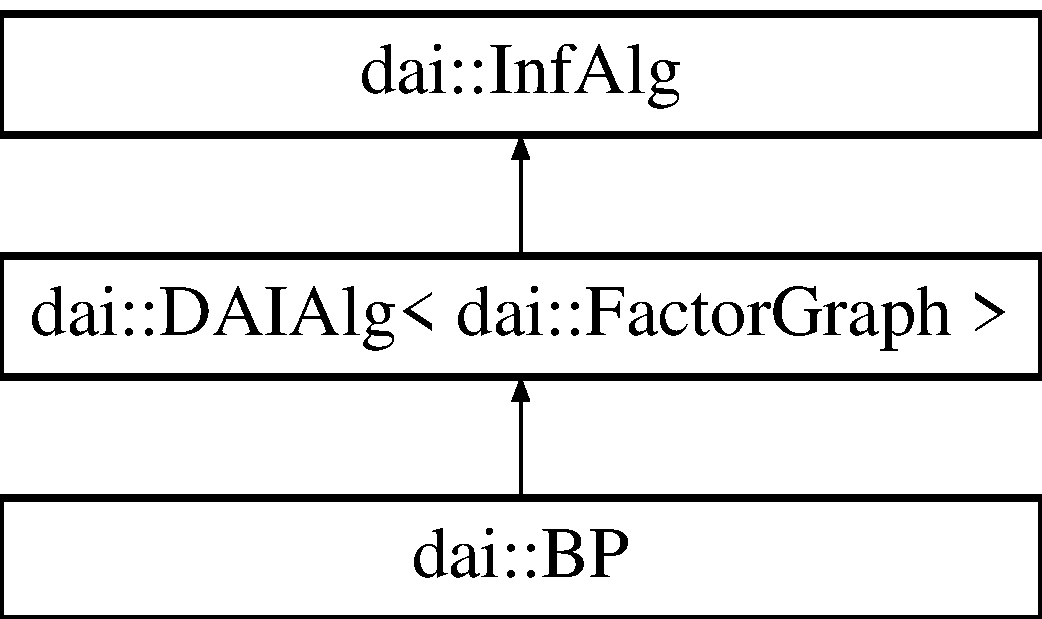
\includegraphics[height=3cm]{classdai_1_1BP}
\end{center}
\end{figure}


\subsection{Detailed Description}
Approximate inference algorithm \char`\"{}(Loopy) Belief Propagation\char`\"{}. \subsection*{Public Member Functions}
\begin{CompactItemize}
\item 
\hypertarget{classdai_1_1BP_79a81420bd4370cdaad9d6a8d85c83a5}{
\hyperlink{classdai_1_1BP_79a81420bd4370cdaad9d6a8d85c83a5}{BP} ()}
\label{classdai_1_1BP_79a81420bd4370cdaad9d6a8d85c83a5}

\begin{CompactList}\small\item\em Default constructor. \item\end{CompactList}\item 
\hypertarget{classdai_1_1BP_e8480cbb4a614119a211ffc03221ba47}{
\hyperlink{classdai_1_1BP_e8480cbb4a614119a211ffc03221ba47}{BP} (const \hyperlink{classdai_1_1BP}{BP} \&x)}
\label{classdai_1_1BP_e8480cbb4a614119a211ffc03221ba47}

\begin{CompactList}\small\item\em Copy constructor. \item\end{CompactList}\item 
\hypertarget{classdai_1_1BP_ba6124da6c2a11b01c0f66cbe8ae9562}{
\hyperlink{classdai_1_1BP}{BP} \& \hyperlink{classdai_1_1BP_ba6124da6c2a11b01c0f66cbe8ae9562}{operator=} (const \hyperlink{classdai_1_1BP}{BP} \&x)}
\label{classdai_1_1BP_ba6124da6c2a11b01c0f66cbe8ae9562}

\begin{CompactList}\small\item\em Assignment operator. \item\end{CompactList}\item 
\hypertarget{classdai_1_1BP_cdfb5e4da942d55f02540d7a5fc29145}{
\hyperlink{classdai_1_1BP_cdfb5e4da942d55f02540d7a5fc29145}{BP} (const \hyperlink{classdai_1_1FactorGraph}{FactorGraph} \&fg, const \hyperlink{classdai_1_1PropertySet}{PropertySet} \&opts)}
\label{classdai_1_1BP_cdfb5e4da942d55f02540d7a5fc29145}

\begin{CompactList}\small\item\em Construct from \hyperlink{classdai_1_1FactorGraph}{FactorGraph} fg and \hyperlink{classdai_1_1PropertySet}{PropertySet} opts. \item\end{CompactList}\item 
\hypertarget{classdai_1_1DAIAlg_48ba6a58d10b8802d690e5e92ec5abe9}{
void \hyperlink{classdai_1_1DAIAlg_48ba6a58d10b8802d690e5e92ec5abe9}{backupFactor} (size\_\-t I)}
\label{classdai_1_1DAIAlg_48ba6a58d10b8802d690e5e92ec5abe9}

\begin{CompactList}\small\item\em Save factor I. \item\end{CompactList}\item 
\hypertarget{classdai_1_1DAIAlg_0176904d3b4b9d083288ea8c4a2dc8bc}{
void \hyperlink{classdai_1_1DAIAlg_0176904d3b4b9d083288ea8c4a2dc8bc}{backupFactors} (const \hyperlink{classdai_1_1VarSet}{VarSet} \&ns)}
\label{classdai_1_1DAIAlg_0176904d3b4b9d083288ea8c4a2dc8bc}

\begin{CompactList}\small\item\em Save Factors involving ns. \item\end{CompactList}\item 
\hypertarget{classdai_1_1DAIAlg_bf8dbd2797ec871e86566a6dfc0864e3}{
void \hyperlink{classdai_1_1DAIAlg_bf8dbd2797ec871e86566a6dfc0864e3}{restoreFactor} (size\_\-t I)}
\label{classdai_1_1DAIAlg_bf8dbd2797ec871e86566a6dfc0864e3}

\begin{CompactList}\small\item\em Restore factor I. \item\end{CompactList}\item 
\hypertarget{classdai_1_1DAIAlg_3ce97e9370f1cdc785526c1a6c1eaadf}{
void \hyperlink{classdai_1_1DAIAlg_3ce97e9370f1cdc785526c1a6c1eaadf}{restoreFactors} (const \hyperlink{classdai_1_1VarSet}{VarSet} \&ns)}
\label{classdai_1_1DAIAlg_3ce97e9370f1cdc785526c1a6c1eaadf}

\begin{CompactList}\small\item\em Restore Factors involving ns. \item\end{CompactList}\item 
\hypertarget{classdai_1_1DAIAlg_b7d537f1a9d116617d8dce722ce65dc0}{
void \hyperlink{classdai_1_1DAIAlg_b7d537f1a9d116617d8dce722ce65dc0}{clamp} (const \hyperlink{classdai_1_1Var}{Var} \&n, size\_\-t i, bool backup=false)}
\label{classdai_1_1DAIAlg_b7d537f1a9d116617d8dce722ce65dc0}

\begin{CompactList}\small\item\em Clamp variable n to value i (i.e. multiply with a Kronecker delta $\delta_{x_n, i}$). \item\end{CompactList}\item 
\hypertarget{classdai_1_1DAIAlg_7f0b8452352080a1e35ab9a68cb589fd}{
void \hyperlink{classdai_1_1DAIAlg_7f0b8452352080a1e35ab9a68cb589fd}{makeCavity} (size\_\-t i, bool backup=false)}
\label{classdai_1_1DAIAlg_7f0b8452352080a1e35ab9a68cb589fd}

\begin{CompactList}\small\item\em Set all factors interacting with var(i) to 1. \item\end{CompactList}\item 
\hypertarget{classdai_1_1DAIAlg_9348542c22d04ed804388f1fe3009fa3}{
\hyperlink{classdai_1_1FactorGraph}{FactorGraph} \& \hyperlink{classdai_1_1DAIAlg_9348542c22d04ed804388f1fe3009fa3}{fg} ()}
\label{classdai_1_1DAIAlg_9348542c22d04ed804388f1fe3009fa3}

\begin{CompactList}\small\item\em Get reference to underlying \hyperlink{classdai_1_1FactorGraph}{FactorGraph}. \item\end{CompactList}\item 
\hypertarget{classdai_1_1DAIAlg_35400e471b8c3c98bef6c74ceac8fa16}{
const \hyperlink{classdai_1_1FactorGraph}{FactorGraph} \& \hyperlink{classdai_1_1DAIAlg_35400e471b8c3c98bef6c74ceac8fa16}{fg} () const }
\label{classdai_1_1DAIAlg_35400e471b8c3c98bef6c74ceac8fa16}

\begin{CompactList}\small\item\em Get const reference to underlying \hyperlink{classdai_1_1FactorGraph}{FactorGraph}. \item\end{CompactList}\end{CompactItemize}
\begin{Indent}{\bf General InfAlg interface}\par
\begin{CompactItemize}
\item 
\hypertarget{classdai_1_1BP_fedbd91bf39951ac3efca096183d6b48}{
virtual \hyperlink{classdai_1_1BP}{BP} $\ast$ \hyperlink{classdai_1_1BP_fedbd91bf39951ac3efca096183d6b48}{clone} () const }
\label{classdai_1_1BP_fedbd91bf39951ac3efca096183d6b48}

\begin{CompactList}\small\item\em Returns a pointer to a new, cloned copy of $\ast$this (i.e., virtual copy constructor). \item\end{CompactList}\item 
\hypertarget{classdai_1_1BP_43d048b5417b74f94eca669eca5eead4}{
virtual \hyperlink{classdai_1_1BP}{BP} $\ast$ \hyperlink{classdai_1_1BP_43d048b5417b74f94eca669eca5eead4}{create} () const }
\label{classdai_1_1BP_43d048b5417b74f94eca669eca5eead4}

\begin{CompactList}\small\item\em Returns a pointer to a newly constructed object $\ast$this (i.e., virtual default constructor). \item\end{CompactList}\item 
\hypertarget{classdai_1_1BP_79d6acb552bc11638fe46dc5a6f68c4d}{
virtual std::string \hyperlink{classdai_1_1BP_79d6acb552bc11638fe46dc5a6f68c4d}{identify} () const }
\label{classdai_1_1BP_79d6acb552bc11638fe46dc5a6f68c4d}

\begin{CompactList}\small\item\em Identifies itself for logging purposes. \item\end{CompactList}\item 
\hypertarget{classdai_1_1BP_1ff12f6f4b486bd53a46a12f7956c99c}{
virtual \hyperlink{classdai_1_1TFactor}{Factor} \hyperlink{classdai_1_1BP_1ff12f6f4b486bd53a46a12f7956c99c}{belief} (const \hyperlink{classdai_1_1Var}{Var} \&n) const }
\label{classdai_1_1BP_1ff12f6f4b486bd53a46a12f7956c99c}

\begin{CompactList}\small\item\em Returns the \char`\"{}belief\char`\"{} (i.e., approximate marginal probability distribution) of a variable. \item\end{CompactList}\item 
\hypertarget{classdai_1_1BP_a898556d97635bfba7227dfa9c0fbdfc}{
virtual \hyperlink{classdai_1_1TFactor}{Factor} \hyperlink{classdai_1_1BP_a898556d97635bfba7227dfa9c0fbdfc}{belief} (const \hyperlink{classdai_1_1VarSet}{VarSet} \&ns) const }
\label{classdai_1_1BP_a898556d97635bfba7227dfa9c0fbdfc}

\begin{CompactList}\small\item\em Returns the \char`\"{}belief\char`\"{} (i.e., approximate marginal probability distribution) of a set of variables. \item\end{CompactList}\item 
\hypertarget{classdai_1_1BP_9abc95e4018fa099278fcdbf8a7941b4}{
virtual std::vector$<$ \hyperlink{classdai_1_1TFactor}{Factor} $>$ \hyperlink{classdai_1_1BP_9abc95e4018fa099278fcdbf8a7941b4}{beliefs} () const }
\label{classdai_1_1BP_9abc95e4018fa099278fcdbf8a7941b4}

\begin{CompactList}\small\item\em Returns all \char`\"{}beliefs\char`\"{} (i.e., approximate marginal probability distribution) calculated by the algorithm. \item\end{CompactList}\item 
\hypertarget{classdai_1_1BP_ed06ca9607cb04cfeb05909366d179ce}{
virtual \hyperlink{namespacedai_e7d0472fdc89a8635825d01940e91cbf}{Real} \hyperlink{classdai_1_1BP_ed06ca9607cb04cfeb05909366d179ce}{logZ} () const }
\label{classdai_1_1BP_ed06ca9607cb04cfeb05909366d179ce}

\begin{CompactList}\small\item\em Returns the logarithm of the (approximated) partition sum (normalizing constant of the factor graph). \item\end{CompactList}\item 
virtual void \hyperlink{classdai_1_1BP_83349319b22a2d71b1f4ef39709365f9}{init} ()
\begin{CompactList}\small\item\em Initializes all data structures of the approximate inference algorithm. \item\end{CompactList}\item 
virtual void \hyperlink{classdai_1_1BP_b711dcd5db848b6d993fac482b64ee20}{init} (const \hyperlink{classdai_1_1VarSet}{VarSet} \&ns)
\begin{CompactList}\small\item\em Initializes all data structures corresponding to some set of variables. \item\end{CompactList}\item 
\hypertarget{classdai_1_1BP_65e6e4e56d227a17d086c5fc8931d3ff}{
virtual double \hyperlink{classdai_1_1BP_65e6e4e56d227a17d086c5fc8931d3ff}{run} ()}
\label{classdai_1_1BP_65e6e4e56d227a17d086c5fc8931d3ff}

\begin{CompactList}\small\item\em Runs the approximate inference algorithm. \item\end{CompactList}\item 
virtual double \hyperlink{classdai_1_1BP_9954b795f95ae1730d4e09a06afd8ee4}{maxDiff} () const 
\item 
virtual size\_\-t \hyperlink{classdai_1_1BP_be6cbc2992d38144198c8f4ea731a26e}{Iterations} () const 
\end{CompactItemize}
\end{Indent}
\begin{Indent}{\bf Additional interface specific for BP}\par
\begin{CompactItemize}
\item 
\hypertarget{classdai_1_1BP_a50b2f745fa1d796e6889f2db581a473}{
\hyperlink{classdai_1_1TFactor}{Factor} \textbf{beliefV} (size\_\-t i) const }
\label{classdai_1_1BP_a50b2f745fa1d796e6889f2db581a473}

\item 
\hypertarget{classdai_1_1BP_fbb68a79c555fac628c5fb79b9c45790}{
\hyperlink{classdai_1_1TFactor}{Factor} \textbf{beliefF} (size\_\-t I) const }
\label{classdai_1_1BP_fbb68a79c555fac628c5fb79b9c45790}

\end{CompactItemize}
\end{Indent}
\subsection*{Public Attributes}
\begin{CompactItemize}
\item 
\hypertarget{classdai_1_1BP_ba42a6eb1857b7f18f5072a25800ae63}{
struct \hyperlink{structdai_1_1BP_1_1Properties}{dai::BP::Properties} \hyperlink{classdai_1_1BP_ba42a6eb1857b7f18f5072a25800ae63}{props}}
\label{classdai_1_1BP_ba42a6eb1857b7f18f5072a25800ae63}

\begin{CompactList}\small\item\em Parameters of this inference algorithm. \item\end{CompactList}\end{CompactItemize}
\subsection*{Static Public Attributes}
\begin{CompactItemize}
\item 
\hypertarget{classdai_1_1BP_f40ab22b371e927fd728569fdbcc607a}{
static const char $\ast$ \hyperlink{classdai_1_1BP_f40ab22b371e927fd728569fdbcc607a}{Name} = \char`\"{}BP\char`\"{}}
\label{classdai_1_1BP_f40ab22b371e927fd728569fdbcc607a}

\begin{CompactList}\small\item\em Name of this inference algorithm. \item\end{CompactList}\end{CompactItemize}
\subsection*{Classes}
\begin{CompactItemize}
\item 
struct \textbf{EdgeProp}
\item 
struct \hyperlink{structdai_1_1BP_1_1Properties}{Properties}
\begin{CompactList}\small\item\em Parameters of this inference algorithm. \item\end{CompactList}\end{CompactItemize}


\subsection{Member Function Documentation}
\hypertarget{classdai_1_1BP_83349319b22a2d71b1f4ef39709365f9}{
\index{dai::BP@{dai::BP}!init@{init}}
\index{init@{init}!dai::BP@{dai::BP}}
\subsubsection[init]{\setlength{\rightskip}{0pt plus 5cm}void dai::BP::init ()\hspace{0.3cm}{\tt  \mbox{[}virtual\mbox{]}}}}
\label{classdai_1_1BP_83349319b22a2d71b1f4ef39709365f9}


Initializes all data structures of the approximate inference algorithm. 

This method should be called at least once before \hyperlink{classdai_1_1BP_65e6e4e56d227a17d086c5fc8931d3ff}{run()} is called 

Implements \hyperlink{classdai_1_1InfAlg_99dd53d1aaccf09a4b977a49a983cc85}{dai::InfAlg}.\hypertarget{classdai_1_1BP_b711dcd5db848b6d993fac482b64ee20}{
\index{dai::BP@{dai::BP}!init@{init}}
\index{init@{init}!dai::BP@{dai::BP}}
\subsubsection[init]{\setlength{\rightskip}{0pt plus 5cm}void dai::BP::init (const {\bf VarSet} \& {\em ns})\hspace{0.3cm}{\tt  \mbox{[}virtual\mbox{]}}}}
\label{classdai_1_1BP_b711dcd5db848b6d993fac482b64ee20}


Initializes all data structures corresponding to some set of variables. 

This method can be used to do a partial initialization after a part of the factor graph has changed. Instead of initializing all data structures, it only initializes those involving the variables in ns. 

Implements \hyperlink{classdai_1_1InfAlg_7d006e89e01a2f3e2a40b0f7f6e37ae5}{dai::InfAlg}.\hypertarget{classdai_1_1BP_9954b795f95ae1730d4e09a06afd8ee4}{
\index{dai::BP@{dai::BP}!maxDiff@{maxDiff}}
\index{maxDiff@{maxDiff}!dai::BP@{dai::BP}}
\subsubsection[maxDiff]{\setlength{\rightskip}{0pt plus 5cm}virtual double dai::BP::maxDiff () const\hspace{0.3cm}{\tt  \mbox{[}inline, virtual\mbox{]}}}}
\label{classdai_1_1BP_9954b795f95ae1730d4e09a06afd8ee4}


Return maximum difference between single node beliefs in the last pass \begin{Desc}
\item[Exceptions:]
\begin{description}
\item[{\em \hyperlink{classdai_1_1Exception}{Exception}}]if not implemented/supported \end{description}
\end{Desc}


Implements \hyperlink{classdai_1_1InfAlg_7e1ca7da15403d5d2af4a855186c0b46}{dai::InfAlg}.\hypertarget{classdai_1_1BP_be6cbc2992d38144198c8f4ea731a26e}{
\index{dai::BP@{dai::BP}!Iterations@{Iterations}}
\index{Iterations@{Iterations}!dai::BP@{dai::BP}}
\subsubsection[Iterations]{\setlength{\rightskip}{0pt plus 5cm}virtual size\_\-t dai::BP::Iterations () const\hspace{0.3cm}{\tt  \mbox{[}inline, virtual\mbox{]}}}}
\label{classdai_1_1BP_be6cbc2992d38144198c8f4ea731a26e}


Return number of passes over the factorgraph \begin{Desc}
\item[Exceptions:]
\begin{description}
\item[{\em \hyperlink{classdai_1_1Exception}{Exception}}]if not implemented/supported \end{description}
\end{Desc}


Implements \hyperlink{classdai_1_1InfAlg_7a93807863cc0a2025c1a78bdf1e14b8}{dai::InfAlg}.

The documentation for this class was generated from the following files:\begin{CompactItemize}
\item 
include/dai/\hyperlink{bp_8h}{bp.h}\item 
src/bp.cpp\end{CompactItemize}

\hypertarget{structdai_1_1BP_1_1Properties}{
\section{dai::BP::Properties Struct Reference}
\label{structdai_1_1BP_1_1Properties}\index{dai::BP::Properties@{dai::BP::Properties}}
}
{\tt \#include $<$dai/bp.h$>$}



\subsection{Detailed Description}
Parameters of this inference algorithm. \subsection*{Public Attributes}
\begin{CompactItemize}
\item 
size\_\-t \hyperlink{structdai_1_1BP_1_1Properties_d9c97ddfdf7a2dc1de3eafe8d57b61ee}{verbose}
\begin{CompactList}\small\item\em Enumeration of possible update schedules. \item\end{CompactList}\item 
\hypertarget{structdai_1_1BP_1_1Properties_d6b27ba966d824597b805d9bc8226f72}{
size\_\-t \hyperlink{structdai_1_1BP_1_1Properties_d6b27ba966d824597b805d9bc8226f72}{maxiter}}
\label{structdai_1_1BP_1_1Properties_d6b27ba966d824597b805d9bc8226f72}

\begin{CompactList}\small\item\em Maximum number of iterations. \item\end{CompactList}\item 
\hypertarget{structdai_1_1BP_1_1Properties_6e47e4800d489c1d213f1d9a0781deac}{
double \hyperlink{structdai_1_1BP_1_1Properties_6e47e4800d489c1d213f1d9a0781deac}{tol}}
\label{structdai_1_1BP_1_1Properties_6e47e4800d489c1d213f1d9a0781deac}

\begin{CompactList}\small\item\em Tolerance. \item\end{CompactList}\item 
\hypertarget{structdai_1_1BP_1_1Properties_71181d319e94f063c6a2fddb591a2b1a}{
bool \hyperlink{structdai_1_1BP_1_1Properties_71181d319e94f063c6a2fddb591a2b1a}{logdomain}}
\label{structdai_1_1BP_1_1Properties_71181d319e94f063c6a2fddb591a2b1a}

\begin{CompactList}\small\item\em Do updates in logarithmic domain? \item\end{CompactList}\item 
\hypertarget{structdai_1_1BP_1_1Properties_c36caab04a3fe03e198842fc7e04a9bc}{
double \hyperlink{structdai_1_1BP_1_1Properties_c36caab04a3fe03e198842fc7e04a9bc}{damping}}
\label{structdai_1_1BP_1_1Properties_c36caab04a3fe03e198842fc7e04a9bc}

\begin{CompactList}\small\item\em Damping constant. \item\end{CompactList}\item 
\hypertarget{structdai_1_1BP_1_1Properties_4e08295ab9d02c28a73270f16ab8f7b7}{
UpdateType \hyperlink{structdai_1_1BP_1_1Properties_4e08295ab9d02c28a73270f16ab8f7b7}{updates}}
\label{structdai_1_1BP_1_1Properties_4e08295ab9d02c28a73270f16ab8f7b7}

\begin{CompactList}\small\item\em Update schedule. \item\end{CompactList}\item 
\hypertarget{structdai_1_1BP_1_1Properties_85f4804c6f8d3579a61ccb3aa3cf454d}{
InfType \hyperlink{structdai_1_1BP_1_1Properties_85f4804c6f8d3579a61ccb3aa3cf454d}{inference}}
\label{structdai_1_1BP_1_1Properties_85f4804c6f8d3579a61ccb3aa3cf454d}

\begin{CompactList}\small\item\em Type of inference: sum-product or max-product? \item\end{CompactList}\end{CompactItemize}


\subsection{Member Data Documentation}
\hypertarget{structdai_1_1BP_1_1Properties_d9c97ddfdf7a2dc1de3eafe8d57b61ee}{
\index{dai::BP::Properties@{dai::BP::Properties}!verbose@{verbose}}
\index{verbose@{verbose}!dai::BP::Properties@{dai::BP::Properties}}
\subsubsection[verbose]{\setlength{\rightskip}{0pt plus 5cm}size\_\-t {\bf dai::BP::Properties::verbose}}}
\label{structdai_1_1BP_1_1Properties_d9c97ddfdf7a2dc1de3eafe8d57b61ee}


Enumeration of possible update schedules. 

Enumeration of inference variants Verbosity 

The documentation for this struct was generated from the following file:\begin{CompactItemize}
\item 
include/dai/\hyperlink{bp_8h}{bp.h}\end{CompactItemize}

\hypertarget{classdai_1_1ClusterGraph}{
\section{dai::ClusterGraph Class Reference}
\label{classdai_1_1ClusterGraph}\index{dai::ClusterGraph@{dai::ClusterGraph}}
}
{\tt \#include $<$dai/clustergraph.h$>$}



\subsection{Detailed Description}
A \hyperlink{classdai_1_1ClusterGraph}{ClusterGraph} is a hypergraph with VarSets as nodes. 

It is implemented as bipartite graph with variable (\hyperlink{classdai_1_1Var}{Var}) nodes and cluster (\hyperlink{classdai_1_1VarSet}{VarSet}) nodes. \subsection*{Public Types}
\begin{CompactItemize}
\item 
\hypertarget{classdai_1_1ClusterGraph_f3157e5f5baf0f36a8c37c43c4a70818}{
typedef \hyperlink{structdai_1_1BipartiteGraph_1_1Neighbor}{BipartiteGraph::Neighbor} \hyperlink{classdai_1_1ClusterGraph_f3157e5f5baf0f36a8c37c43c4a70818}{Neighbor}}
\label{classdai_1_1ClusterGraph_f3157e5f5baf0f36a8c37c43c4a70818}

\begin{CompactList}\small\item\em Shorthand for \hyperlink{structdai_1_1BipartiteGraph_1_1Neighbor}{BipartiteGraph::Neighbor}. \item\end{CompactList}\item 
\hypertarget{classdai_1_1ClusterGraph_c5d233b46473ce14c1773db35cb8100d}{
typedef \hyperlink{classdai_1_1BipartiteGraph_ff511d0eba0fd2956c08b602029ba95f}{BipartiteGraph::Edge} \hyperlink{classdai_1_1ClusterGraph_c5d233b46473ce14c1773db35cb8100d}{Edge}}
\label{classdai_1_1ClusterGraph_c5d233b46473ce14c1773db35cb8100d}

\begin{CompactList}\small\item\em Shorthand for \hyperlink{classdai_1_1BipartiteGraph_ff511d0eba0fd2956c08b602029ba95f}{BipartiteGraph::Edge}. \item\end{CompactList}\end{CompactItemize}
\subsection*{Public Member Functions}
\begin{CompactItemize}
\item 
\hypertarget{classdai_1_1ClusterGraph_d2e6d97e39753c1524026e8dbe52387a}{
\hyperlink{classdai_1_1ClusterGraph_d2e6d97e39753c1524026e8dbe52387a}{ClusterGraph} ()}
\label{classdai_1_1ClusterGraph_d2e6d97e39753c1524026e8dbe52387a}

\begin{CompactList}\small\item\em Default constructor. \item\end{CompactList}\item 
\hypertarget{classdai_1_1ClusterGraph_5509e79c9c41d7219104eaf07fce6a36}{
\hyperlink{classdai_1_1ClusterGraph_5509e79c9c41d7219104eaf07fce6a36}{ClusterGraph} (const std::vector$<$ \hyperlink{classdai_1_1VarSet}{VarSet} $>$ \&cls)}
\label{classdai_1_1ClusterGraph_5509e79c9c41d7219104eaf07fce6a36}

\begin{CompactList}\small\item\em Construct from vector$<$VarSet$>$. \item\end{CompactList}\item 
\hypertarget{classdai_1_1ClusterGraph_591f12b43ccc7d0f046169c03d61c948}{
\hyperlink{classdai_1_1ClusterGraph_591f12b43ccc7d0f046169c03d61c948}{ClusterGraph} (const \hyperlink{classdai_1_1ClusterGraph}{ClusterGraph} \&x)}
\label{classdai_1_1ClusterGraph_591f12b43ccc7d0f046169c03d61c948}

\begin{CompactList}\small\item\em Copy constructor. \item\end{CompactList}\item 
\hypertarget{classdai_1_1ClusterGraph_6397064f5586477caff7d3aec485248f}{
\hyperlink{classdai_1_1ClusterGraph}{ClusterGraph} \& \hyperlink{classdai_1_1ClusterGraph_6397064f5586477caff7d3aec485248f}{operator=} (const \hyperlink{classdai_1_1ClusterGraph}{ClusterGraph} \&x)}
\label{classdai_1_1ClusterGraph_6397064f5586477caff7d3aec485248f}

\begin{CompactList}\small\item\em Assignment operator. \item\end{CompactList}\item 
\hypertarget{classdai_1_1ClusterGraph_768d5b0b1636909630dfca1a0f4df878}{
bool \hyperlink{classdai_1_1ClusterGraph_768d5b0b1636909630dfca1a0f4df878}{isMaximal} (size\_\-t I) const }
\label{classdai_1_1ClusterGraph_768d5b0b1636909630dfca1a0f4df878}

\begin{CompactList}\small\item\em Returns true if cluster I is not contained in a larger cluster. \item\end{CompactList}\item 
\hypertarget{classdai_1_1ClusterGraph_13cfa2d4973d387d55ba0a54d4676a6e}{
\hyperlink{classdai_1_1ClusterGraph}{ClusterGraph} \& \hyperlink{classdai_1_1ClusterGraph_13cfa2d4973d387d55ba0a54d4676a6e}{eraseNonMaximal} ()}
\label{classdai_1_1ClusterGraph_13cfa2d4973d387d55ba0a54d4676a6e}

\begin{CompactList}\small\item\em Erases all VarSets that are not maximal. \item\end{CompactList}\item 
\hypertarget{classdai_1_1ClusterGraph_6a3592792de64c05211abc9aebf525d2}{
size\_\-t \hyperlink{classdai_1_1ClusterGraph_6a3592792de64c05211abc9aebf525d2}{size} () const }
\label{classdai_1_1ClusterGraph_6a3592792de64c05211abc9aebf525d2}

\begin{CompactList}\small\item\em Returns number of clusters. \item\end{CompactList}\item 
\hypertarget{classdai_1_1ClusterGraph_bd0f148c5953b0ec4340e1b1c37ab0ef}{
size\_\-t \hyperlink{classdai_1_1ClusterGraph_bd0f148c5953b0ec4340e1b1c37ab0ef}{findVar} (const \hyperlink{classdai_1_1Var}{Var} \&n) const }
\label{classdai_1_1ClusterGraph_bd0f148c5953b0ec4340e1b1c37ab0ef}

\begin{CompactList}\small\item\em Returns index of variable n. \item\end{CompactList}\item 
\hypertarget{classdai_1_1ClusterGraph_b193856e886cf22d9773282dd4a01f20}{
bool \hyperlink{classdai_1_1ClusterGraph_b193856e886cf22d9773282dd4a01f20}{adj} (size\_\-t i1, size\_\-t i2)}
\label{classdai_1_1ClusterGraph_b193856e886cf22d9773282dd4a01f20}

\begin{CompactList}\small\item\em Returns true if vars with indices i1 and i2 are adjacent, i.e., both contained in the same cluster. \item\end{CompactList}\item 
\hypertarget{classdai_1_1ClusterGraph_bcb07aa0dd6b564c9af98f07ff3a486e}{
\hyperlink{classdai_1_1VarSet}{VarSet} \hyperlink{classdai_1_1ClusterGraph_bcb07aa0dd6b564c9af98f07ff3a486e}{Delta} (size\_\-t i) const }
\label{classdai_1_1ClusterGraph_bcb07aa0dd6b564c9af98f07ff3a486e}

\begin{CompactList}\small\item\em Returns union of clusters that contain the variable with index i. \item\end{CompactList}\item 
\hypertarget{classdai_1_1ClusterGraph_da8f45f04be422aaf399e02565013d6c}{
void \hyperlink{classdai_1_1ClusterGraph_da8f45f04be422aaf399e02565013d6c}{insert} (const \hyperlink{classdai_1_1VarSet}{VarSet} \&cl)}
\label{classdai_1_1ClusterGraph_da8f45f04be422aaf399e02565013d6c}

\begin{CompactList}\small\item\em Inserts a cluster (if it does not already exist). \item\end{CompactList}\item 
\hypertarget{classdai_1_1ClusterGraph_407cabb372ced5d4399cea029f1e1bf0}{
\hyperlink{classdai_1_1VarSet}{VarSet} \hyperlink{classdai_1_1ClusterGraph_407cabb372ced5d4399cea029f1e1bf0}{delta} (size\_\-t i) const }
\label{classdai_1_1ClusterGraph_407cabb372ced5d4399cea029f1e1bf0}

\begin{CompactList}\small\item\em Returns union of clusters that contain variable with index i, minus this variable. \item\end{CompactList}\item 
\hypertarget{classdai_1_1ClusterGraph_21a1a08351c17c90a3efac6a5f8a4818}{
\hyperlink{classdai_1_1ClusterGraph}{ClusterGraph} \& \hyperlink{classdai_1_1ClusterGraph_21a1a08351c17c90a3efac6a5f8a4818}{eraseSubsuming} (size\_\-t i)}
\label{classdai_1_1ClusterGraph_21a1a08351c17c90a3efac6a5f8a4818}

\begin{CompactList}\small\item\em Erases all clusters that contain n where n is the variable with index i. \item\end{CompactList}\item 
\hypertarget{classdai_1_1ClusterGraph_bb5e88ece31a9a7ff405f988dc1a1e46}{
const std::vector$<$ \hyperlink{classdai_1_1VarSet}{VarSet} $>$ \& \hyperlink{classdai_1_1ClusterGraph_bb5e88ece31a9a7ff405f988dc1a1e46}{toVector} () const }
\label{classdai_1_1ClusterGraph_bb5e88ece31a9a7ff405f988dc1a1e46}

\begin{CompactList}\small\item\em Returns a const reference to the clusters. \item\end{CompactList}\item 
size\_\-t \hyperlink{classdai_1_1ClusterGraph_517e9ea33d7ec133586110eb5106fcc4}{eliminationCost} (size\_\-t i)
\begin{CompactList}\small\item\em Calculates cost of eliminating the variable with index i. \item\end{CompactList}\item 
\hypertarget{classdai_1_1ClusterGraph_1ec39220612d165fc15dde360b57bf46}{
\hyperlink{classdai_1_1ClusterGraph}{ClusterGraph} \hyperlink{classdai_1_1ClusterGraph_1ec39220612d165fc15dde360b57bf46}{VarElim} (const std::vector$<$ \hyperlink{classdai_1_1Var}{Var} $>$ \&ElimSeq) const }
\label{classdai_1_1ClusterGraph_1ec39220612d165fc15dde360b57bf46}

\begin{CompactList}\small\item\em Performs Variable Elimination without Probs, i.e. only keeping track of. \item\end{CompactList}\item 
\hypertarget{classdai_1_1ClusterGraph_742b9a4367bf6ce1a6a05e58b9892089}{
\hyperlink{classdai_1_1ClusterGraph}{ClusterGraph} \hyperlink{classdai_1_1ClusterGraph_742b9a4367bf6ce1a6a05e58b9892089}{VarElim\_\-MinFill} () const }
\label{classdai_1_1ClusterGraph_742b9a4367bf6ce1a6a05e58b9892089}

\begin{CompactList}\small\item\em Performs Variable Eliminiation using the MinFill heuristic. \item\end{CompactList}\end{CompactItemize}
\subsection*{Public Attributes}
\begin{CompactItemize}
\item 
\hypertarget{classdai_1_1ClusterGraph_d8a1a655cf546d42303d46f3d08079cc}{
\hyperlink{classdai_1_1BipartiteGraph}{BipartiteGraph} \hyperlink{classdai_1_1ClusterGraph_d8a1a655cf546d42303d46f3d08079cc}{G}}
\label{classdai_1_1ClusterGraph_d8a1a655cf546d42303d46f3d08079cc}

\begin{CompactList}\small\item\em Stores the neighborhood structure. \item\end{CompactList}\item 
\hypertarget{classdai_1_1ClusterGraph_b96a722f403754e0437c5fbe0c364f57}{
std::vector$<$ \hyperlink{classdai_1_1Var}{Var} $>$ \hyperlink{classdai_1_1ClusterGraph_b96a722f403754e0437c5fbe0c364f57}{vars}}
\label{classdai_1_1ClusterGraph_b96a722f403754e0437c5fbe0c364f57}

\begin{CompactList}\small\item\em Stores the variables corresponding to the nodes. \item\end{CompactList}\item 
\hypertarget{classdai_1_1ClusterGraph_cf58184945136e95a49177c52da8d2c2}{
std::vector$<$ \hyperlink{classdai_1_1VarSet}{VarSet} $>$ \hyperlink{classdai_1_1ClusterGraph_cf58184945136e95a49177c52da8d2c2}{clusters}}
\label{classdai_1_1ClusterGraph_cf58184945136e95a49177c52da8d2c2}

\begin{CompactList}\small\item\em Stores the clusters corresponding to the hyperedges. \item\end{CompactList}\end{CompactItemize}
\subsection*{Friends}
\begin{CompactItemize}
\item 
\hypertarget{classdai_1_1ClusterGraph_23a45a96ea996832c667d346c99bc760}{
std::ostream \& \hyperlink{classdai_1_1ClusterGraph_23a45a96ea996832c667d346c99bc760}{operator$<$$<$} (std::ostream \&os, const \hyperlink{classdai_1_1ClusterGraph}{ClusterGraph} \&cl)}
\label{classdai_1_1ClusterGraph_23a45a96ea996832c667d346c99bc760}

\begin{CompactList}\small\item\em Writes a \hyperlink{classdai_1_1ClusterGraph}{ClusterGraph} to an output stream. \item\end{CompactList}\end{CompactItemize}


\subsection{Member Function Documentation}
\hypertarget{classdai_1_1ClusterGraph_517e9ea33d7ec133586110eb5106fcc4}{
\index{dai::ClusterGraph@{dai::ClusterGraph}!eliminationCost@{eliminationCost}}
\index{eliminationCost@{eliminationCost}!dai::ClusterGraph@{dai::ClusterGraph}}
\subsubsection[eliminationCost]{\setlength{\rightskip}{0pt plus 5cm}size\_\-t dai::ClusterGraph::eliminationCost (size\_\-t {\em i})\hspace{0.3cm}{\tt  \mbox{[}inline\mbox{]}}}}
\label{classdai_1_1ClusterGraph_517e9ea33d7ec133586110eb5106fcc4}


Calculates cost of eliminating the variable with index i. 

The cost is measured as \char`\"{}number of added edges in the adjacency graph\char`\"{}, where the adjacency graph has the variables as its nodes and connects nodes i1 and i2 iff i1 and i2 occur in some common cluster. 

The documentation for this class was generated from the following files:\begin{CompactItemize}
\item 
include/dai/\hyperlink{clustergraph_8h}{clustergraph.h}\item 
src/clustergraph.cpp\end{CompactItemize}

\hypertarget{classdai_1_1DAIAlg}{
\section{dai::DAIAlg$<$ GRM $>$ Class Template Reference}
\label{classdai_1_1DAIAlg}\index{dai::DAIAlg@{dai::DAIAlg}}
}
{\tt \#include $<$dai/daialg.h$>$}

Inheritance diagram for dai::DAIAlg$<$ GRM $>$::\begin{figure}[H]
\begin{center}
\leavevmode
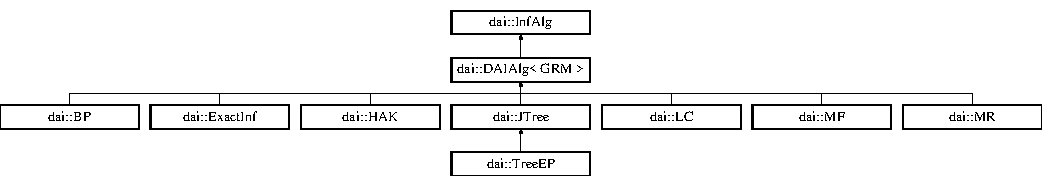
\includegraphics[height=2.37037cm]{classdai_1_1DAIAlg}
\end{center}
\end{figure}


\subsection{Detailed Description}
\subsubsection*{template$<$class GRM$>$ class dai::DAIAlg$<$ GRM $>$}

Combines an \hyperlink{classdai_1_1InfAlg}{InfAlg} and a graphical model, e.g., a \hyperlink{classdai_1_1FactorGraph}{FactorGraph} or \hyperlink{classdai_1_1RegionGraph}{RegionGraph}. 

\begin{Desc}
\item[Template Parameters:]
\begin{description}
\item[{\em GRM}]Should be castable to \hyperlink{classdai_1_1FactorGraph}{FactorGraph} \end{description}
\end{Desc}
\subsection*{Public Member Functions}
\begin{CompactItemize}
\item 
\hypertarget{classdai_1_1DAIAlg_1b66918854e70f19c8b506658c9f50e0}{
\hyperlink{classdai_1_1DAIAlg_1b66918854e70f19c8b506658c9f50e0}{DAIAlg} ()}
\label{classdai_1_1DAIAlg_1b66918854e70f19c8b506658c9f50e0}

\begin{CompactList}\small\item\em Default constructor. \item\end{CompactList}\item 
\hypertarget{classdai_1_1DAIAlg_46ac57c2abad7c6870f30edc951aeff3}{
\hyperlink{classdai_1_1DAIAlg_46ac57c2abad7c6870f30edc951aeff3}{DAIAlg} (const GRM \&grm)}
\label{classdai_1_1DAIAlg_46ac57c2abad7c6870f30edc951aeff3}

\begin{CompactList}\small\item\em Construct from GRM. \item\end{CompactList}\item 
\hypertarget{classdai_1_1DAIAlg_3223cf97a6e3dc25e8aec7f4c3e22d0b}{
\hyperlink{classdai_1_1DAIAlg_3223cf97a6e3dc25e8aec7f4c3e22d0b}{DAIAlg} (const \hyperlink{classdai_1_1DAIAlg}{DAIAlg} \&x)}
\label{classdai_1_1DAIAlg_3223cf97a6e3dc25e8aec7f4c3e22d0b}

\begin{CompactList}\small\item\em Copy constructor. \item\end{CompactList}\item 
\hypertarget{classdai_1_1DAIAlg_364afd19b16ac9233fd4b235b76317c8}{
\hyperlink{classdai_1_1DAIAlg}{DAIAlg} \& \hyperlink{classdai_1_1DAIAlg_364afd19b16ac9233fd4b235b76317c8}{operator=} (const \hyperlink{classdai_1_1DAIAlg}{DAIAlg} \&x)}
\label{classdai_1_1DAIAlg_364afd19b16ac9233fd4b235b76317c8}

\begin{CompactList}\small\item\em Assignment operator. \item\end{CompactList}\item 
\hypertarget{classdai_1_1DAIAlg_48ba6a58d10b8802d690e5e92ec5abe9}{
void \hyperlink{classdai_1_1DAIAlg_48ba6a58d10b8802d690e5e92ec5abe9}{backupFactor} (size\_\-t I)}
\label{classdai_1_1DAIAlg_48ba6a58d10b8802d690e5e92ec5abe9}

\begin{CompactList}\small\item\em Save factor I. \item\end{CompactList}\item 
\hypertarget{classdai_1_1DAIAlg_0176904d3b4b9d083288ea8c4a2dc8bc}{
void \hyperlink{classdai_1_1DAIAlg_0176904d3b4b9d083288ea8c4a2dc8bc}{backupFactors} (const \hyperlink{classdai_1_1VarSet}{VarSet} \&ns)}
\label{classdai_1_1DAIAlg_0176904d3b4b9d083288ea8c4a2dc8bc}

\begin{CompactList}\small\item\em Save Factors involving ns. \item\end{CompactList}\item 
\hypertarget{classdai_1_1DAIAlg_bf8dbd2797ec871e86566a6dfc0864e3}{
void \hyperlink{classdai_1_1DAIAlg_bf8dbd2797ec871e86566a6dfc0864e3}{restoreFactor} (size\_\-t I)}
\label{classdai_1_1DAIAlg_bf8dbd2797ec871e86566a6dfc0864e3}

\begin{CompactList}\small\item\em Restore factor I. \item\end{CompactList}\item 
\hypertarget{classdai_1_1DAIAlg_3ce97e9370f1cdc785526c1a6c1eaadf}{
void \hyperlink{classdai_1_1DAIAlg_3ce97e9370f1cdc785526c1a6c1eaadf}{restoreFactors} (const \hyperlink{classdai_1_1VarSet}{VarSet} \&ns)}
\label{classdai_1_1DAIAlg_3ce97e9370f1cdc785526c1a6c1eaadf}

\begin{CompactList}\small\item\em Restore Factors involving ns. \item\end{CompactList}\item 
\hypertarget{classdai_1_1DAIAlg_b7d537f1a9d116617d8dce722ce65dc0}{
void \hyperlink{classdai_1_1DAIAlg_b7d537f1a9d116617d8dce722ce65dc0}{clamp} (const \hyperlink{classdai_1_1Var}{Var} \&n, size\_\-t i, bool backup=false)}
\label{classdai_1_1DAIAlg_b7d537f1a9d116617d8dce722ce65dc0}

\begin{CompactList}\small\item\em Clamp variable n to value i (i.e. multiply with a Kronecker delta $\delta_{x_n, i}$). \item\end{CompactList}\item 
\hypertarget{classdai_1_1DAIAlg_7f0b8452352080a1e35ab9a68cb589fd}{
void \hyperlink{classdai_1_1DAIAlg_7f0b8452352080a1e35ab9a68cb589fd}{makeCavity} (size\_\-t i, bool backup=false)}
\label{classdai_1_1DAIAlg_7f0b8452352080a1e35ab9a68cb589fd}

\begin{CompactList}\small\item\em Set all factors interacting with var(i) to 1. \item\end{CompactList}\item 
\hypertarget{classdai_1_1DAIAlg_9348542c22d04ed804388f1fe3009fa3}{
\hyperlink{classdai_1_1FactorGraph}{FactorGraph} \& \hyperlink{classdai_1_1DAIAlg_9348542c22d04ed804388f1fe3009fa3}{fg} ()}
\label{classdai_1_1DAIAlg_9348542c22d04ed804388f1fe3009fa3}

\begin{CompactList}\small\item\em Get reference to underlying \hyperlink{classdai_1_1FactorGraph}{FactorGraph}. \item\end{CompactList}\item 
\hypertarget{classdai_1_1DAIAlg_35400e471b8c3c98bef6c74ceac8fa16}{
const \hyperlink{classdai_1_1FactorGraph}{FactorGraph} \& \hyperlink{classdai_1_1DAIAlg_35400e471b8c3c98bef6c74ceac8fa16}{fg} () const }
\label{classdai_1_1DAIAlg_35400e471b8c3c98bef6c74ceac8fa16}

\begin{CompactList}\small\item\em Get const reference to underlying \hyperlink{classdai_1_1FactorGraph}{FactorGraph}. \item\end{CompactList}\item 
\hypertarget{classdai_1_1InfAlg_28fd90657745e2a150f94d22319c6e2d}{
virtual \hyperlink{classdai_1_1InfAlg}{InfAlg} $\ast$ \hyperlink{classdai_1_1InfAlg_28fd90657745e2a150f94d22319c6e2d}{clone} () const =0}
\label{classdai_1_1InfAlg_28fd90657745e2a150f94d22319c6e2d}

\begin{CompactList}\small\item\em Returns a pointer to a new, cloned copy of $\ast$this (i.e., virtual copy constructor). \item\end{CompactList}\item 
\hypertarget{classdai_1_1InfAlg_48936a6f22a324cbe22d553ea41de7e2}{
virtual \hyperlink{classdai_1_1InfAlg}{InfAlg} $\ast$ \hyperlink{classdai_1_1InfAlg_48936a6f22a324cbe22d553ea41de7e2}{create} () const =0}
\label{classdai_1_1InfAlg_48936a6f22a324cbe22d553ea41de7e2}

\begin{CompactList}\small\item\em Returns a pointer to a newly constructed object $\ast$this (i.e., virtual default constructor). \item\end{CompactList}\item 
\hypertarget{classdai_1_1InfAlg_2f84c282ef54ab76e70fba6f823f2b27}{
virtual std::string \hyperlink{classdai_1_1InfAlg_2f84c282ef54ab76e70fba6f823f2b27}{identify} () const =0}
\label{classdai_1_1InfAlg_2f84c282ef54ab76e70fba6f823f2b27}

\begin{CompactList}\small\item\em Identifies itself for logging purposes. \item\end{CompactList}\item 
\hypertarget{classdai_1_1InfAlg_d8d8f71ea44c71905e9ee9531e3de48f}{
virtual \hyperlink{classdai_1_1TFactor}{Factor} \hyperlink{classdai_1_1InfAlg_d8d8f71ea44c71905e9ee9531e3de48f}{belief} (const \hyperlink{classdai_1_1Var}{Var} \&n) const =0}
\label{classdai_1_1InfAlg_d8d8f71ea44c71905e9ee9531e3de48f}

\begin{CompactList}\small\item\em Returns the \char`\"{}belief\char`\"{} (i.e., approximate marginal probability distribution) of a variable. \item\end{CompactList}\item 
\hypertarget{classdai_1_1InfAlg_74028032f667c44b0437019c4c13360b}{
virtual \hyperlink{classdai_1_1TFactor}{Factor} \hyperlink{classdai_1_1InfAlg_74028032f667c44b0437019c4c13360b}{belief} (const \hyperlink{classdai_1_1VarSet}{VarSet} \&n) const =0}
\label{classdai_1_1InfAlg_74028032f667c44b0437019c4c13360b}

\begin{CompactList}\small\item\em Returns the \char`\"{}belief\char`\"{} (i.e., approximate marginal probability distribution) of a set of variables. \item\end{CompactList}\item 
\hypertarget{classdai_1_1InfAlg_eac9f6b52ff7a11a1e5ac2c03bbd6eb0}{
virtual std::vector$<$ \hyperlink{classdai_1_1TFactor}{Factor} $>$ \hyperlink{classdai_1_1InfAlg_eac9f6b52ff7a11a1e5ac2c03bbd6eb0}{beliefs} () const =0}
\label{classdai_1_1InfAlg_eac9f6b52ff7a11a1e5ac2c03bbd6eb0}

\begin{CompactList}\small\item\em Returns all \char`\"{}beliefs\char`\"{} (i.e., approximate marginal probability distribution) calculated by the algorithm. \item\end{CompactList}\item 
\hypertarget{classdai_1_1InfAlg_40a2353d63c358ebca834d40b0a4fc70}{
virtual \hyperlink{namespacedai_e7d0472fdc89a8635825d01940e91cbf}{Real} \hyperlink{classdai_1_1InfAlg_40a2353d63c358ebca834d40b0a4fc70}{logZ} () const =0}
\label{classdai_1_1InfAlg_40a2353d63c358ebca834d40b0a4fc70}

\begin{CompactList}\small\item\em Returns the logarithm of the (approximated) partition sum (normalizing constant of the factor graph). \item\end{CompactList}\item 
virtual void \hyperlink{classdai_1_1InfAlg_99dd53d1aaccf09a4b977a49a983cc85}{init} ()=0
\begin{CompactList}\small\item\em Initializes all data structures of the approximate inference algorithm. \item\end{CompactList}\item 
virtual void \hyperlink{classdai_1_1InfAlg_7d006e89e01a2f3e2a40b0f7f6e37ae5}{init} (const \hyperlink{classdai_1_1VarSet}{VarSet} \&ns)=0
\begin{CompactList}\small\item\em Initializes all data structures corresponding to some set of variables. \item\end{CompactList}\item 
\hypertarget{classdai_1_1InfAlg_6b169737c142ff0be5db3dab4f4eb568}{
virtual double \hyperlink{classdai_1_1InfAlg_6b169737c142ff0be5db3dab4f4eb568}{run} ()=0}
\label{classdai_1_1InfAlg_6b169737c142ff0be5db3dab4f4eb568}

\begin{CompactList}\small\item\em Runs the approximate inference algorithm. \item\end{CompactList}\item 
virtual double \hyperlink{classdai_1_1InfAlg_7e1ca7da15403d5d2af4a855186c0b46}{maxDiff} () const =0
\item 
virtual size\_\-t \hyperlink{classdai_1_1InfAlg_7a93807863cc0a2025c1a78bdf1e14b8}{Iterations} () const =0
\end{CompactItemize}


\subsection{Member Function Documentation}
\hypertarget{classdai_1_1InfAlg_99dd53d1aaccf09a4b977a49a983cc85}{
\index{dai::DAIAlg@{dai::DAIAlg}!init@{init}}
\index{init@{init}!dai::DAIAlg@{dai::DAIAlg}}
\subsubsection[init]{\setlength{\rightskip}{0pt plus 5cm}virtual void dai::InfAlg::init ()\hspace{0.3cm}{\tt  \mbox{[}pure virtual, inherited\mbox{]}}}}
\label{classdai_1_1InfAlg_99dd53d1aaccf09a4b977a49a983cc85}


Initializes all data structures of the approximate inference algorithm. 

This method should be called at least once before \hyperlink{classdai_1_1InfAlg_6b169737c142ff0be5db3dab4f4eb568}{run()} is called 

Implemented in \hyperlink{classdai_1_1BP_83349319b22a2d71b1f4ef39709365f9}{dai::BP}, \hyperlink{classdai_1_1ExactInf_8b86be92502af6ef5ecb38f12406733d}{dai::ExactInf}, \hyperlink{classdai_1_1HAK_b30055f32f2c9a84d76668ff74606697}{dai::HAK}, \hyperlink{classdai_1_1JTree_cbb2df1dc4e64097a46fc4cb1394e76f}{dai::JTree}, \hyperlink{classdai_1_1LC_007ab11f0d08d0ed23ae141230b122cc}{dai::LC}, \hyperlink{classdai_1_1MF_eb993d502d0cb97424ebff82e0cf6839}{dai::MF}, \hyperlink{classdai_1_1MR_859f5c780ec490232dc7a2b8f11da38b}{dai::MR}, and \hyperlink{classdai_1_1TreeEP_fff5580fa87ce391223a2e2867527248}{dai::TreeEP}.\hypertarget{classdai_1_1InfAlg_7d006e89e01a2f3e2a40b0f7f6e37ae5}{
\index{dai::DAIAlg@{dai::DAIAlg}!init@{init}}
\index{init@{init}!dai::DAIAlg@{dai::DAIAlg}}
\subsubsection[init]{\setlength{\rightskip}{0pt plus 5cm}virtual void dai::InfAlg::init (const {\bf VarSet} \& {\em ns})\hspace{0.3cm}{\tt  \mbox{[}pure virtual, inherited\mbox{]}}}}
\label{classdai_1_1InfAlg_7d006e89e01a2f3e2a40b0f7f6e37ae5}


Initializes all data structures corresponding to some set of variables. 

This method can be used to do a partial initialization after a part of the factor graph has changed. Instead of initializing all data structures, it only initializes those involving the variables in ns. 

Implemented in \hyperlink{classdai_1_1BP_b711dcd5db848b6d993fac482b64ee20}{dai::BP}, \hyperlink{classdai_1_1ExactInf_ace58f99e40bb4084c73d6b77fd26456}{dai::ExactInf}, \hyperlink{classdai_1_1HAK_53cd01bc1e70859d556ac71b5e25a192}{dai::HAK}, \hyperlink{classdai_1_1JTree_365c52b5f264c844ac5c010026719350}{dai::JTree}, \hyperlink{classdai_1_1LC_b077c808ad6ca6b9e134746d0846ea5d}{dai::LC}, \hyperlink{classdai_1_1MF_49ddd5c9c9f51ee9fb5e153b7194ac71}{dai::MF}, \hyperlink{classdai_1_1MR_da0e0829e87b541633dbb6078529c21d}{dai::MR}, and \hyperlink{classdai_1_1TreeEP_3cc3718d1fbdf67db23a846283f99d08}{dai::TreeEP}.\hypertarget{classdai_1_1InfAlg_7e1ca7da15403d5d2af4a855186c0b46}{
\index{dai::DAIAlg@{dai::DAIAlg}!maxDiff@{maxDiff}}
\index{maxDiff@{maxDiff}!dai::DAIAlg@{dai::DAIAlg}}
\subsubsection[maxDiff]{\setlength{\rightskip}{0pt plus 5cm}virtual double dai::InfAlg::maxDiff () const\hspace{0.3cm}{\tt  \mbox{[}pure virtual, inherited\mbox{]}}}}
\label{classdai_1_1InfAlg_7e1ca7da15403d5d2af4a855186c0b46}


Return maximum difference between single node beliefs in the last pass \begin{Desc}
\item[Exceptions:]
\begin{description}
\item[{\em \hyperlink{classdai_1_1Exception}{Exception}}]if not implemented/supported \end{description}
\end{Desc}


Implemented in \hyperlink{classdai_1_1BP_9954b795f95ae1730d4e09a06afd8ee4}{dai::BP}, \hyperlink{classdai_1_1ExactInf_4f3189ff1567e80dd245a1308f1f31bf}{dai::ExactInf}, \hyperlink{classdai_1_1HAK_1eb4c5a84c30f7c8db8b8f4c0c54f567}{dai::HAK}, \hyperlink{classdai_1_1JTree_acd3916835c9d349aa1b22a2dd54de83}{dai::JTree}, \hyperlink{classdai_1_1LC_32b30963958c3f408d1c5a618fcf418d}{dai::LC}, \hyperlink{classdai_1_1MF_032b149026f011a5cbcd01eb08a3b8dc}{dai::MF}, \hyperlink{classdai_1_1MR_a55d0a62912e9fe8a685157cfa309918}{dai::MR}, and \hyperlink{classdai_1_1TreeEP_d1214cd7bc0899d1a8dc4523bacdb488}{dai::TreeEP}.\hypertarget{classdai_1_1InfAlg_7a93807863cc0a2025c1a78bdf1e14b8}{
\index{dai::DAIAlg@{dai::DAIAlg}!Iterations@{Iterations}}
\index{Iterations@{Iterations}!dai::DAIAlg@{dai::DAIAlg}}
\subsubsection[Iterations]{\setlength{\rightskip}{0pt plus 5cm}virtual size\_\-t dai::InfAlg::Iterations () const\hspace{0.3cm}{\tt  \mbox{[}pure virtual, inherited\mbox{]}}}}
\label{classdai_1_1InfAlg_7a93807863cc0a2025c1a78bdf1e14b8}


Return number of passes over the factorgraph \begin{Desc}
\item[Exceptions:]
\begin{description}
\item[{\em \hyperlink{classdai_1_1Exception}{Exception}}]if not implemented/supported \end{description}
\end{Desc}


Implemented in \hyperlink{classdai_1_1BP_be6cbc2992d38144198c8f4ea731a26e}{dai::BP}, \hyperlink{classdai_1_1ExactInf_2df22866419ee923043c8fcf0a2ff62b}{dai::ExactInf}, \hyperlink{classdai_1_1HAK_27599fc844670e503786ac5d485713c5}{dai::HAK}, \hyperlink{classdai_1_1JTree_71cd98f072d69f6ce60af8b52ef02eb8}{dai::JTree}, \hyperlink{classdai_1_1LC_8654c28fad78fa6cd850b2207b271086}{dai::LC}, \hyperlink{classdai_1_1MF_e2daf3cd007572d19d6156f2484db4fd}{dai::MF}, \hyperlink{classdai_1_1MR_6a199aa1d43b3c143a4b631735f53ee3}{dai::MR}, and \hyperlink{classdai_1_1TreeEP_e18e681d1f078e42445d39f8605df7d4}{dai::TreeEP}.

The documentation for this class was generated from the following file:\begin{CompactItemize}
\item 
include/dai/\hyperlink{daialg_8h}{daialg.h}\end{CompactItemize}

\hypertarget{classdai_1_1DEdge}{
\section{dai::DEdge Class Reference}
\label{classdai_1_1DEdge}\index{dai::DEdge@{dai::DEdge}}
}
{\tt \#include $<$dai/weightedgraph.h$>$}



\subsection{Detailed Description}
Represents a directed edge pointing from n1 to n2. \subsection*{Public Member Functions}
\begin{CompactItemize}
\item 
\hypertarget{classdai_1_1DEdge_f5427cbe19ce225fe7b56dd2d035a7a0}{
\hyperlink{classdai_1_1DEdge_f5427cbe19ce225fe7b56dd2d035a7a0}{DEdge} ()}
\label{classdai_1_1DEdge_f5427cbe19ce225fe7b56dd2d035a7a0}

\begin{CompactList}\small\item\em Default constructor. \item\end{CompactList}\item 
\hypertarget{classdai_1_1DEdge_0936737355725c765b6902303fb75b04}{
\hyperlink{classdai_1_1DEdge_0936737355725c765b6902303fb75b04}{DEdge} (size\_\-t m1, size\_\-t m2)}
\label{classdai_1_1DEdge_0936737355725c765b6902303fb75b04}

\begin{CompactList}\small\item\em Constructor. \item\end{CompactList}\item 
\hypertarget{classdai_1_1DEdge_ac85e6f5aa72f552c3d6a6fd7941d2db}{
bool \hyperlink{classdai_1_1DEdge_ac85e6f5aa72f552c3d6a6fd7941d2db}{operator==} (const \hyperlink{classdai_1_1DEdge}{DEdge} \&x) const }
\label{classdai_1_1DEdge_ac85e6f5aa72f552c3d6a6fd7941d2db}

\begin{CompactList}\small\item\em Tests for equality. \item\end{CompactList}\item 
\hypertarget{classdai_1_1DEdge_a13e5a5126ff6c0b754af96349c8f613}{
bool \hyperlink{classdai_1_1DEdge_a13e5a5126ff6c0b754af96349c8f613}{operator!=} (const \hyperlink{classdai_1_1DEdge}{DEdge} \&x) const }
\label{classdai_1_1DEdge_a13e5a5126ff6c0b754af96349c8f613}

\begin{CompactList}\small\item\em Tests for inequality. \item\end{CompactList}\item 
\hypertarget{classdai_1_1DEdge_b2378683166fd3eb5518edce5823c1ed}{
bool \hyperlink{classdai_1_1DEdge_b2378683166fd3eb5518edce5823c1ed}{operator$<$} (const \hyperlink{classdai_1_1DEdge}{DEdge} \&x) const }
\label{classdai_1_1DEdge_b2378683166fd3eb5518edce5823c1ed}

\begin{CompactList}\small\item\em Smaller-than operator (performs lexicographical comparison). \item\end{CompactList}\end{CompactItemize}
\subsection*{Public Attributes}
\begin{CompactItemize}
\item 
\hypertarget{classdai_1_1DEdge_7e45508d3b566c073f176ea845497c0d}{
size\_\-t \hyperlink{classdai_1_1DEdge_7e45508d3b566c073f176ea845497c0d}{n1}}
\label{classdai_1_1DEdge_7e45508d3b566c073f176ea845497c0d}

\begin{CompactList}\small\item\em First node index. \item\end{CompactList}\item 
\hypertarget{classdai_1_1DEdge_0836ffc192d1e2ebdac4d4e8242feb38}{
size\_\-t \hyperlink{classdai_1_1DEdge_0836ffc192d1e2ebdac4d4e8242feb38}{n2}}
\label{classdai_1_1DEdge_0836ffc192d1e2ebdac4d4e8242feb38}

\begin{CompactList}\small\item\em Second node index. \item\end{CompactList}\end{CompactItemize}
\subsection*{Friends}
\begin{CompactItemize}
\item 
\hypertarget{classdai_1_1DEdge_c12ac5065e77dc3040d464405fe1f609}{
std::ostream \& \hyperlink{classdai_1_1DEdge_c12ac5065e77dc3040d464405fe1f609}{operator$<$$<$} (std::ostream \&os, const \hyperlink{classdai_1_1DEdge}{DEdge} \&e)}
\label{classdai_1_1DEdge_c12ac5065e77dc3040d464405fe1f609}

\begin{CompactList}\small\item\em Writes a \hyperlink{classdai_1_1DEdge}{DEdge} to an output stream. \item\end{CompactList}\end{CompactItemize}


The documentation for this class was generated from the following file:\begin{CompactItemize}
\item 
include/dai/\hyperlink{weightedgraph_8h}{weightedgraph.h}\end{CompactItemize}

\hypertarget{classdai_1_1Diffs}{
\section{dai::Diffs Class Reference}
\label{classdai_1_1Diffs}\index{dai::Diffs@{dai::Diffs}}
}
{\tt \#include $<$dai/util.h$>$}

Inherits std::vector$<$ double $>$.



\subsection{Detailed Description}
Used to keep track of the progress made by iterative algorithms. \subsection*{Public Member Functions}
\begin{CompactItemize}
\item 
\hypertarget{classdai_1_1Diffs_4b57c2ecdc2b6d70c404824330876235}{
\hyperlink{classdai_1_1Diffs_4b57c2ecdc2b6d70c404824330876235}{Diffs} (long maxsize, double def)}
\label{classdai_1_1Diffs_4b57c2ecdc2b6d70c404824330876235}

\begin{CompactList}\small\item\em Constructor. \item\end{CompactList}\item 
\hypertarget{classdai_1_1Diffs_b6d18664bd4f72da5b7105a0791c21fe}{
double \hyperlink{classdai_1_1Diffs_b6d18664bd4f72da5b7105a0791c21fe}{maxDiff} ()}
\label{classdai_1_1Diffs_b6d18664bd4f72da5b7105a0791c21fe}

\begin{CompactList}\small\item\em Returns maximum difference encountered. \item\end{CompactList}\item 
\hypertarget{classdai_1_1Diffs_badc1817a2021474a11c5296c4d6cf7c}{
void \hyperlink{classdai_1_1Diffs_badc1817a2021474a11c5296c4d6cf7c}{push} (double x)}
\label{classdai_1_1Diffs_badc1817a2021474a11c5296c4d6cf7c}

\begin{CompactList}\small\item\em Register new difference x. \item\end{CompactList}\item 
\hypertarget{classdai_1_1Diffs_2833e1db5b0b3661ad7d4bdbfb00f9c6}{
size\_\-t \hyperlink{classdai_1_1Diffs_2833e1db5b0b3661ad7d4bdbfb00f9c6}{maxSize} ()}
\label{classdai_1_1Diffs_2833e1db5b0b3661ad7d4bdbfb00f9c6}

\begin{CompactList}\small\item\em Return maximum number of differences stored. \item\end{CompactList}\end{CompactItemize}


The documentation for this class was generated from the following file:\begin{CompactItemize}
\item 
include/dai/\hyperlink{util_8h}{util.h}\end{CompactItemize}

\hypertarget{classdai_1_1ExactInf}{
\section{dai::ExactInf Class Reference}
\label{classdai_1_1ExactInf}\index{dai::ExactInf@{dai::ExactInf}}
}
{\tt \#include $<$dai/exactinf.h$>$}

Inheritance diagram for dai::ExactInf::\begin{figure}[H]
\begin{center}
\leavevmode
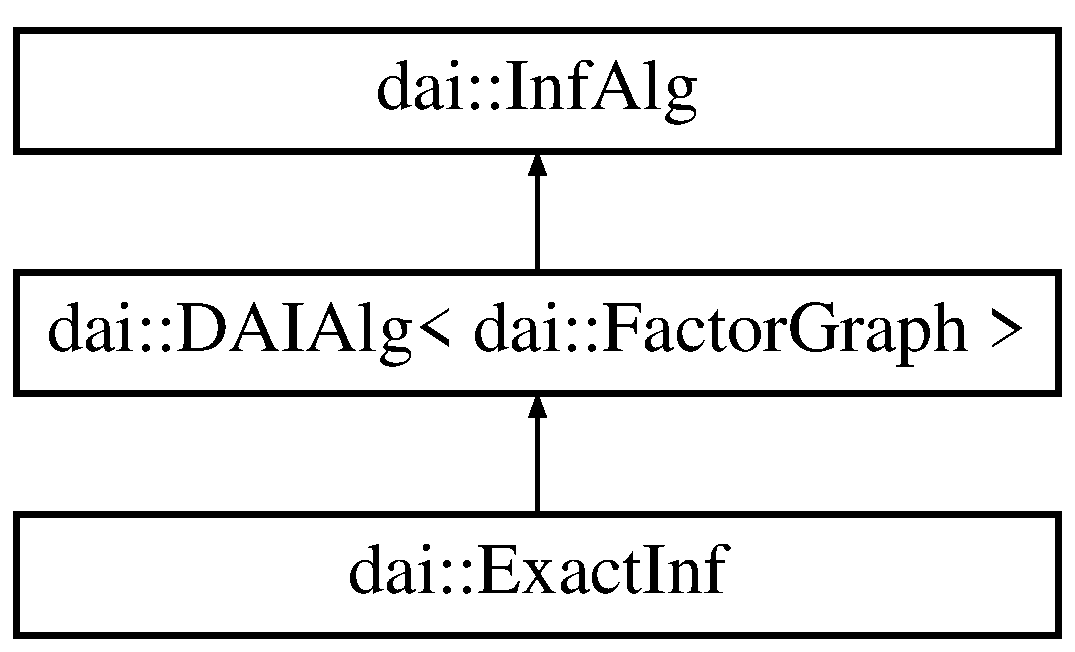
\includegraphics[height=3cm]{classdai_1_1ExactInf}
\end{center}
\end{figure}


\subsection{Detailed Description}
Exact inference algorithm using brute force enumeration (mainly useful for testing purposes). \subsection*{Public Member Functions}
\begin{CompactItemize}
\item 
\hypertarget{classdai_1_1ExactInf_324505f8fdc4904179eb2e1c96fccda1}{
\hyperlink{classdai_1_1ExactInf_324505f8fdc4904179eb2e1c96fccda1}{ExactInf} ()}
\label{classdai_1_1ExactInf_324505f8fdc4904179eb2e1c96fccda1}

\begin{CompactList}\small\item\em Default constructor. \item\end{CompactList}\item 
\hypertarget{classdai_1_1ExactInf_4eb13120c5f7f4d58333117a9ca1033d}{
\hyperlink{classdai_1_1ExactInf_4eb13120c5f7f4d58333117a9ca1033d}{ExactInf} (const \hyperlink{classdai_1_1ExactInf}{ExactInf} \&x)}
\label{classdai_1_1ExactInf_4eb13120c5f7f4d58333117a9ca1033d}

\begin{CompactList}\small\item\em Copy constructor. \item\end{CompactList}\item 
\hypertarget{classdai_1_1ExactInf_59fcfa39f061f0ee326a5e0593ef598e}{
\hyperlink{classdai_1_1ExactInf}{ExactInf} \& \hyperlink{classdai_1_1ExactInf_59fcfa39f061f0ee326a5e0593ef598e}{operator=} (const \hyperlink{classdai_1_1ExactInf}{ExactInf} \&x)}
\label{classdai_1_1ExactInf_59fcfa39f061f0ee326a5e0593ef598e}

\begin{CompactList}\small\item\em Assignment operator. \item\end{CompactList}\item 
\hypertarget{classdai_1_1ExactInf_014dde3f2b7ec66332fb1cbe00538b89}{
\hyperlink{classdai_1_1ExactInf_014dde3f2b7ec66332fb1cbe00538b89}{ExactInf} (const \hyperlink{classdai_1_1FactorGraph}{FactorGraph} \&fg, const \hyperlink{classdai_1_1PropertySet}{PropertySet} \&opts)}
\label{classdai_1_1ExactInf_014dde3f2b7ec66332fb1cbe00538b89}

\begin{CompactList}\small\item\em Construct from \hyperlink{classdai_1_1FactorGraph}{FactorGraph} fg and \hyperlink{classdai_1_1PropertySet}{PropertySet} opts. \item\end{CompactList}\item 
\hypertarget{classdai_1_1DAIAlg_48ba6a58d10b8802d690e5e92ec5abe9}{
void \hyperlink{classdai_1_1DAIAlg_48ba6a58d10b8802d690e5e92ec5abe9}{backupFactor} (size\_\-t I)}
\label{classdai_1_1DAIAlg_48ba6a58d10b8802d690e5e92ec5abe9}

\begin{CompactList}\small\item\em Save factor I. \item\end{CompactList}\item 
\hypertarget{classdai_1_1DAIAlg_0176904d3b4b9d083288ea8c4a2dc8bc}{
void \hyperlink{classdai_1_1DAIAlg_0176904d3b4b9d083288ea8c4a2dc8bc}{backupFactors} (const \hyperlink{classdai_1_1VarSet}{VarSet} \&ns)}
\label{classdai_1_1DAIAlg_0176904d3b4b9d083288ea8c4a2dc8bc}

\begin{CompactList}\small\item\em Save Factors involving ns. \item\end{CompactList}\item 
\hypertarget{classdai_1_1DAIAlg_bf8dbd2797ec871e86566a6dfc0864e3}{
void \hyperlink{classdai_1_1DAIAlg_bf8dbd2797ec871e86566a6dfc0864e3}{restoreFactor} (size\_\-t I)}
\label{classdai_1_1DAIAlg_bf8dbd2797ec871e86566a6dfc0864e3}

\begin{CompactList}\small\item\em Restore factor I. \item\end{CompactList}\item 
\hypertarget{classdai_1_1DAIAlg_3ce97e9370f1cdc785526c1a6c1eaadf}{
void \hyperlink{classdai_1_1DAIAlg_3ce97e9370f1cdc785526c1a6c1eaadf}{restoreFactors} (const \hyperlink{classdai_1_1VarSet}{VarSet} \&ns)}
\label{classdai_1_1DAIAlg_3ce97e9370f1cdc785526c1a6c1eaadf}

\begin{CompactList}\small\item\em Restore Factors involving ns. \item\end{CompactList}\item 
\hypertarget{classdai_1_1DAIAlg_b7d537f1a9d116617d8dce722ce65dc0}{
void \hyperlink{classdai_1_1DAIAlg_b7d537f1a9d116617d8dce722ce65dc0}{clamp} (const \hyperlink{classdai_1_1Var}{Var} \&n, size\_\-t i, bool backup=false)}
\label{classdai_1_1DAIAlg_b7d537f1a9d116617d8dce722ce65dc0}

\begin{CompactList}\small\item\em Clamp variable n to value i (i.e. multiply with a Kronecker delta $\delta_{x_n, i}$). \item\end{CompactList}\item 
\hypertarget{classdai_1_1DAIAlg_7f0b8452352080a1e35ab9a68cb589fd}{
void \hyperlink{classdai_1_1DAIAlg_7f0b8452352080a1e35ab9a68cb589fd}{makeCavity} (size\_\-t i, bool backup=false)}
\label{classdai_1_1DAIAlg_7f0b8452352080a1e35ab9a68cb589fd}

\begin{CompactList}\small\item\em Set all factors interacting with var(i) to 1. \item\end{CompactList}\item 
\hypertarget{classdai_1_1DAIAlg_9348542c22d04ed804388f1fe3009fa3}{
\hyperlink{classdai_1_1FactorGraph}{FactorGraph} \& \hyperlink{classdai_1_1DAIAlg_9348542c22d04ed804388f1fe3009fa3}{fg} ()}
\label{classdai_1_1DAIAlg_9348542c22d04ed804388f1fe3009fa3}

\begin{CompactList}\small\item\em Get reference to underlying \hyperlink{classdai_1_1FactorGraph}{FactorGraph}. \item\end{CompactList}\item 
\hypertarget{classdai_1_1DAIAlg_35400e471b8c3c98bef6c74ceac8fa16}{
const \hyperlink{classdai_1_1FactorGraph}{FactorGraph} \& \hyperlink{classdai_1_1DAIAlg_35400e471b8c3c98bef6c74ceac8fa16}{fg} () const }
\label{classdai_1_1DAIAlg_35400e471b8c3c98bef6c74ceac8fa16}

\begin{CompactList}\small\item\em Get const reference to underlying \hyperlink{classdai_1_1FactorGraph}{FactorGraph}. \item\end{CompactList}\end{CompactItemize}
\begin{Indent}{\bf General InfAlg interface}\par
\begin{CompactItemize}
\item 
\hypertarget{classdai_1_1ExactInf_ac21e07e94947d380da177523caa0213}{
virtual \hyperlink{classdai_1_1ExactInf}{ExactInf} $\ast$ \hyperlink{classdai_1_1ExactInf_ac21e07e94947d380da177523caa0213}{clone} () const }
\label{classdai_1_1ExactInf_ac21e07e94947d380da177523caa0213}

\begin{CompactList}\small\item\em Returns a pointer to a new, cloned copy of $\ast$this (i.e., virtual copy constructor). \item\end{CompactList}\item 
\hypertarget{classdai_1_1ExactInf_10d22ff1ae94fb7af4a1bca9496e3bce}{
virtual \hyperlink{classdai_1_1ExactInf}{ExactInf} $\ast$ \hyperlink{classdai_1_1ExactInf_10d22ff1ae94fb7af4a1bca9496e3bce}{create} () const }
\label{classdai_1_1ExactInf_10d22ff1ae94fb7af4a1bca9496e3bce}

\begin{CompactList}\small\item\em Returns a pointer to a newly constructed object $\ast$this (i.e., virtual default constructor). \item\end{CompactList}\item 
\hypertarget{classdai_1_1ExactInf_b316d463564eafd5c2629eded1f31b80}{
virtual std::string \hyperlink{classdai_1_1ExactInf_b316d463564eafd5c2629eded1f31b80}{identify} () const }
\label{classdai_1_1ExactInf_b316d463564eafd5c2629eded1f31b80}

\begin{CompactList}\small\item\em Identifies itself for logging purposes. \item\end{CompactList}\item 
\hypertarget{classdai_1_1ExactInf_85d120a9ab1b03ae922be7a7568de64e}{
virtual \hyperlink{classdai_1_1TFactor}{Factor} \hyperlink{classdai_1_1ExactInf_85d120a9ab1b03ae922be7a7568de64e}{belief} (const \hyperlink{classdai_1_1Var}{Var} \&n) const }
\label{classdai_1_1ExactInf_85d120a9ab1b03ae922be7a7568de64e}

\begin{CompactList}\small\item\em Returns the \char`\"{}belief\char`\"{} (i.e., approximate marginal probability distribution) of a variable. \item\end{CompactList}\item 
\hypertarget{classdai_1_1ExactInf_e3f944864f06bacd49fcf7c3f6f2fa20}{
virtual \hyperlink{classdai_1_1TFactor}{Factor} \hyperlink{classdai_1_1ExactInf_e3f944864f06bacd49fcf7c3f6f2fa20}{belief} (const \hyperlink{classdai_1_1VarSet}{VarSet} \&ns) const }
\label{classdai_1_1ExactInf_e3f944864f06bacd49fcf7c3f6f2fa20}

\begin{CompactList}\small\item\em Returns the \char`\"{}belief\char`\"{} (i.e., approximate marginal probability distribution) of a set of variables. \item\end{CompactList}\item 
\hypertarget{classdai_1_1ExactInf_d6ec1824cb811733bfa68071ab4ae5e3}{
virtual std::vector$<$ \hyperlink{classdai_1_1TFactor}{Factor} $>$ \hyperlink{classdai_1_1ExactInf_d6ec1824cb811733bfa68071ab4ae5e3}{beliefs} () const }
\label{classdai_1_1ExactInf_d6ec1824cb811733bfa68071ab4ae5e3}

\begin{CompactList}\small\item\em Returns all \char`\"{}beliefs\char`\"{} (i.e., approximate marginal probability distribution) calculated by the algorithm. \item\end{CompactList}\item 
\hypertarget{classdai_1_1ExactInf_f13ecd0ae1374782ac4afa8c6e679d73}{
virtual \hyperlink{namespacedai_e7d0472fdc89a8635825d01940e91cbf}{Real} \hyperlink{classdai_1_1ExactInf_f13ecd0ae1374782ac4afa8c6e679d73}{logZ} () const }
\label{classdai_1_1ExactInf_f13ecd0ae1374782ac4afa8c6e679d73}

\begin{CompactList}\small\item\em Returns the logarithm of the (approximated) partition sum (normalizing constant of the factor graph). \item\end{CompactList}\item 
virtual void \hyperlink{classdai_1_1ExactInf_8b86be92502af6ef5ecb38f12406733d}{init} ()
\begin{CompactList}\small\item\em Initializes all data structures of the approximate inference algorithm. \item\end{CompactList}\item 
virtual void \hyperlink{classdai_1_1ExactInf_ace58f99e40bb4084c73d6b77fd26456}{init} (const \hyperlink{classdai_1_1VarSet}{VarSet} \&)
\begin{CompactList}\small\item\em Initializes all data structures corresponding to some set of variables. \item\end{CompactList}\item 
\hypertarget{classdai_1_1ExactInf_cfb073de0b7b01929a9d02e6500f2443}{
virtual double \hyperlink{classdai_1_1ExactInf_cfb073de0b7b01929a9d02e6500f2443}{run} ()}
\label{classdai_1_1ExactInf_cfb073de0b7b01929a9d02e6500f2443}

\begin{CompactList}\small\item\em Runs the approximate inference algorithm. \item\end{CompactList}\item 
virtual double \hyperlink{classdai_1_1ExactInf_4f3189ff1567e80dd245a1308f1f31bf}{maxDiff} () const 
\item 
virtual size\_\-t \hyperlink{classdai_1_1ExactInf_2df22866419ee923043c8fcf0a2ff62b}{Iterations} () const 
\end{CompactItemize}
\end{Indent}
\begin{Indent}{\bf Additional interface specific for ExactInf}\par
\begin{CompactItemize}
\item 
\hypertarget{classdai_1_1ExactInf_6a8257999f86bc9aea76c4906eeed7e6}{
\hyperlink{classdai_1_1TFactor}{Factor} \textbf{beliefV} (size\_\-t i) const }
\label{classdai_1_1ExactInf_6a8257999f86bc9aea76c4906eeed7e6}

\item 
\hypertarget{classdai_1_1ExactInf_75fe681325b30f2e8ad643a9273610a7}{
\hyperlink{classdai_1_1TFactor}{Factor} \textbf{beliefF} (size\_\-t I) const }
\label{classdai_1_1ExactInf_75fe681325b30f2e8ad643a9273610a7}

\end{CompactItemize}
\end{Indent}
\subsection*{Public Attributes}
\begin{CompactItemize}
\item 
\hypertarget{classdai_1_1ExactInf_b4dbf2483cfdfbb9971b2f69c42a2327}{
struct \hyperlink{structdai_1_1ExactInf_1_1Properties}{dai::ExactInf::Properties} \hyperlink{classdai_1_1ExactInf_b4dbf2483cfdfbb9971b2f69c42a2327}{props}}
\label{classdai_1_1ExactInf_b4dbf2483cfdfbb9971b2f69c42a2327}

\begin{CompactList}\small\item\em Parameters of this inference algorithm. \item\end{CompactList}\end{CompactItemize}
\subsection*{Static Public Attributes}
\begin{CompactItemize}
\item 
\hypertarget{classdai_1_1ExactInf_2280f2174f843cb88eb715d51536b812}{
static const char $\ast$ \hyperlink{classdai_1_1ExactInf_2280f2174f843cb88eb715d51536b812}{Name} = \char`\"{}EXACT\char`\"{}}
\label{classdai_1_1ExactInf_2280f2174f843cb88eb715d51536b812}

\begin{CompactList}\small\item\em Name of this inference algorithm. \item\end{CompactList}\end{CompactItemize}
\subsection*{Classes}
\begin{CompactItemize}
\item 
struct \hyperlink{structdai_1_1ExactInf_1_1Properties}{Properties}
\begin{CompactList}\small\item\em Parameters of this inference algorithm. \item\end{CompactList}\end{CompactItemize}


\subsection{Member Function Documentation}
\hypertarget{classdai_1_1ExactInf_8b86be92502af6ef5ecb38f12406733d}{
\index{dai::ExactInf@{dai::ExactInf}!init@{init}}
\index{init@{init}!dai::ExactInf@{dai::ExactInf}}
\subsubsection[init]{\setlength{\rightskip}{0pt plus 5cm}void dai::ExactInf::init ()\hspace{0.3cm}{\tt  \mbox{[}virtual\mbox{]}}}}
\label{classdai_1_1ExactInf_8b86be92502af6ef5ecb38f12406733d}


Initializes all data structures of the approximate inference algorithm. 

This method should be called at least once before \hyperlink{classdai_1_1ExactInf_cfb073de0b7b01929a9d02e6500f2443}{run()} is called 

Implements \hyperlink{classdai_1_1InfAlg_99dd53d1aaccf09a4b977a49a983cc85}{dai::InfAlg}.\hypertarget{classdai_1_1ExactInf_ace58f99e40bb4084c73d6b77fd26456}{
\index{dai::ExactInf@{dai::ExactInf}!init@{init}}
\index{init@{init}!dai::ExactInf@{dai::ExactInf}}
\subsubsection[init]{\setlength{\rightskip}{0pt plus 5cm}virtual void dai::ExactInf::init (const {\bf VarSet} \& {\em ns})\hspace{0.3cm}{\tt  \mbox{[}inline, virtual\mbox{]}}}}
\label{classdai_1_1ExactInf_ace58f99e40bb4084c73d6b77fd26456}


Initializes all data structures corresponding to some set of variables. 

This method can be used to do a partial initialization after a part of the factor graph has changed. Instead of initializing all data structures, it only initializes those involving the variables in ns. 

Implements \hyperlink{classdai_1_1InfAlg_7d006e89e01a2f3e2a40b0f7f6e37ae5}{dai::InfAlg}.\hypertarget{classdai_1_1ExactInf_4f3189ff1567e80dd245a1308f1f31bf}{
\index{dai::ExactInf@{dai::ExactInf}!maxDiff@{maxDiff}}
\index{maxDiff@{maxDiff}!dai::ExactInf@{dai::ExactInf}}
\subsubsection[maxDiff]{\setlength{\rightskip}{0pt plus 5cm}virtual double dai::ExactInf::maxDiff () const\hspace{0.3cm}{\tt  \mbox{[}inline, virtual\mbox{]}}}}
\label{classdai_1_1ExactInf_4f3189ff1567e80dd245a1308f1f31bf}


Return maximum difference between single node beliefs in the last pass \begin{Desc}
\item[Exceptions:]
\begin{description}
\item[{\em \hyperlink{classdai_1_1Exception}{Exception}}]if not implemented/supported \end{description}
\end{Desc}


Implements \hyperlink{classdai_1_1InfAlg_7e1ca7da15403d5d2af4a855186c0b46}{dai::InfAlg}.\hypertarget{classdai_1_1ExactInf_2df22866419ee923043c8fcf0a2ff62b}{
\index{dai::ExactInf@{dai::ExactInf}!Iterations@{Iterations}}
\index{Iterations@{Iterations}!dai::ExactInf@{dai::ExactInf}}
\subsubsection[Iterations]{\setlength{\rightskip}{0pt plus 5cm}virtual size\_\-t dai::ExactInf::Iterations () const\hspace{0.3cm}{\tt  \mbox{[}inline, virtual\mbox{]}}}}
\label{classdai_1_1ExactInf_2df22866419ee923043c8fcf0a2ff62b}


Return number of passes over the factorgraph \begin{Desc}
\item[Exceptions:]
\begin{description}
\item[{\em \hyperlink{classdai_1_1Exception}{Exception}}]if not implemented/supported \end{description}
\end{Desc}


Implements \hyperlink{classdai_1_1InfAlg_7a93807863cc0a2025c1a78bdf1e14b8}{dai::InfAlg}.

The documentation for this class was generated from the following files:\begin{CompactItemize}
\item 
include/dai/\hyperlink{exactinf_8h}{exactinf.h}\item 
src/exactinf.cpp\end{CompactItemize}

\hypertarget{structdai_1_1ExactInf_1_1Properties}{
\section{dai::ExactInf::Properties Struct Reference}
\label{structdai_1_1ExactInf_1_1Properties}\index{dai::ExactInf::Properties@{dai::ExactInf::Properties}}
}
{\tt \#include $<$dai/exactinf.h$>$}



\subsection{Detailed Description}
Parameters of this inference algorithm. \subsection*{Public Attributes}
\begin{CompactItemize}
\item 
\hypertarget{structdai_1_1ExactInf_1_1Properties_13f9e5a1531ceeb9537d981da2212075}{
size\_\-t \hyperlink{structdai_1_1ExactInf_1_1Properties_13f9e5a1531ceeb9537d981da2212075}{verbose}}
\label{structdai_1_1ExactInf_1_1Properties_13f9e5a1531ceeb9537d981da2212075}

\begin{CompactList}\small\item\em Verbosity. \item\end{CompactList}\end{CompactItemize}


The documentation for this struct was generated from the following file:\begin{CompactItemize}
\item 
include/dai/\hyperlink{exactinf_8h}{exactinf.h}\end{CompactItemize}

\hypertarget{classdai_1_1Exception}{
\section{dai::Exception Class Reference}
\label{classdai_1_1Exception}\index{dai::Exception@{dai::Exception}}
}
{\tt \#include $<$dai/exceptions.h$>$}

Inherits std::runtime\_\-error.



\subsection{Detailed Description}
Represents an exception (based on std::runtime\_\-error). \subsection*{Public Types}
\begin{CompactItemize}
\item 
enum \hyperlink{classdai_1_1Exception_39671dae0b9533d8ed596927160d023b}{codes} \{ \par
\textbf{NOT\_\-IMPLEMENTED}, 
\textbf{UNKNOWN\_\-DAI\_\-ALGORITHM}, 
\textbf{UNKNOWN\_\-PROPERTY\_\-TYPE}, 
\textbf{MALFORMED\_\-PROPERTY}, 
\par
\textbf{UNKNOWN\_\-ENUM\_\-VALUE}, 
\textbf{CANNOT\_\-READ\_\-FILE}, 
\textbf{CANNOT\_\-WRITE\_\-FILE}, 
\textbf{INVALID\_\-FACTORGRAPH\_\-FILE}, 
\par
\textbf{NOT\_\-ALL\_\-PROPERTIES\_\-SPECIFIED}, 
\textbf{MULTIPLE\_\-UNDO}, 
\textbf{FACTORGRAPH\_\-NOT\_\-CONNECTED}, 
\textbf{IMPOSSIBLE\_\-TYPECAST}, 
\par
\textbf{INTERNAL\_\-ERROR}, 
\textbf{NUM\_\-ERRORS}
 \}
\begin{CompactList}\small\item\em Enumeration of exceptions used in libDAI. \item\end{CompactList}\end{CompactItemize}
\subsection*{Public Member Functions}
\begin{CompactItemize}
\item 
\hypertarget{classdai_1_1Exception_a10fe7cf9d3e20c5aae77f1892554236}{
\hyperlink{classdai_1_1Exception_a10fe7cf9d3e20c5aae77f1892554236}{Exception} (size\_\-t code, const std::string \&msg=\char`\"{}\char`\"{})}
\label{classdai_1_1Exception_a10fe7cf9d3e20c5aae77f1892554236}

\begin{CompactList}\small\item\em Constructor. \item\end{CompactList}\end{CompactItemize}


The documentation for this class was generated from the following files:\begin{CompactItemize}
\item 
include/dai/\hyperlink{exceptions_8h}{exceptions.h}\item 
src/exceptions.cpp\end{CompactItemize}

\hypertarget{classdai_1_1FactorGraph}{
\section{dai::FactorGraph Class Reference}
\label{classdai_1_1FactorGraph}\index{dai::FactorGraph@{dai::FactorGraph}}
}
{\tt \#include $<$dai/factorgraph.h$>$}

Inheritance diagram for dai::FactorGraph::\begin{figure}[H]
\begin{center}
\leavevmode
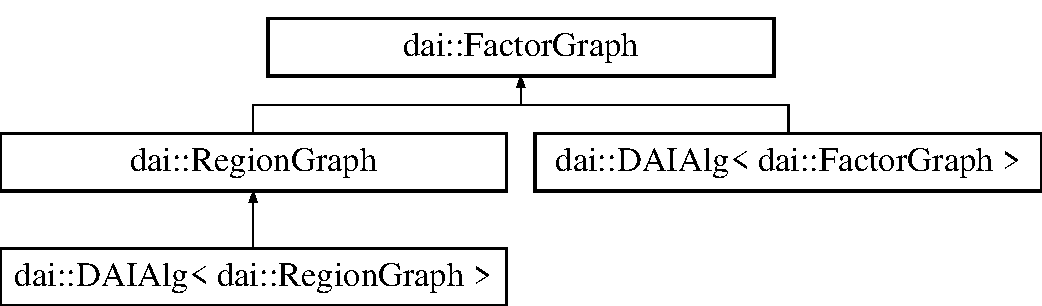
\includegraphics[height=3cm]{classdai_1_1FactorGraph}
\end{center}
\end{figure}


\subsection{Detailed Description}
Represents a factor graph. 

Both Bayesian Networks and Markov random fields can be represented in a unifying representation, called {\em factor graph\/} \mbox{[}\hyperlink{Bibliography_KFL01}{KFL01}\mbox{]}, implemented in libDAI by the \hyperlink{classdai_1_1FactorGraph}{FactorGraph} class.

Consider a probability distribution over $N$ discrete random variables $x_0,x_1,\dots,x_N$ that factorizes as a product of factors, each of which depends on some subset of the variables: \[ P(x_0,x_1,\dots,x_N) = \frac{1}{Z} \prod_{I=0}^M f_I(x_I), \qquad Z = \sum_{x_0}\dots\sum_{x_N} \prod_{I=0}^M f_I(X_I). \] Each factor $f_I$ is a function from an associated subset of variables $X_I \subset \{x_0,x_1,\dots,x_N\}$ to the nonnegative real numbers.

For a Bayesian network, each factor corresponds to a (conditional) probability table, whereas for a Markov random field, each factor corresponds to a maximal clique of the undirected graph.

Factor graphs explicitly express the factorization structure of the corresponding probability distribution. \subsection*{Public Types}
\begin{CompactItemize}
\item 
\hypertarget{classdai_1_1FactorGraph_1552870151bb7f7a88b3120a777c1056}{
typedef \hyperlink{structdai_1_1BipartiteGraph_1_1Neighbor}{BipartiteGraph::Neighbor} \hyperlink{classdai_1_1FactorGraph_1552870151bb7f7a88b3120a777c1056}{Neighbor}}
\label{classdai_1_1FactorGraph_1552870151bb7f7a88b3120a777c1056}

\begin{CompactList}\small\item\em Shorthand for \hyperlink{structdai_1_1BipartiteGraph_1_1Neighbor}{BipartiteGraph::Neighbor}. \item\end{CompactList}\item 
\hypertarget{classdai_1_1FactorGraph_326942db90fe2dbdf99041d5d966019e}{
typedef \hyperlink{classdai_1_1BipartiteGraph_031237b607d2868b80052e71b4149b29}{BipartiteGraph::Neighbors} \hyperlink{classdai_1_1FactorGraph_326942db90fe2dbdf99041d5d966019e}{Neighbors}}
\label{classdai_1_1FactorGraph_326942db90fe2dbdf99041d5d966019e}

\begin{CompactList}\small\item\em Shorthand for \hyperlink{classdai_1_1BipartiteGraph_031237b607d2868b80052e71b4149b29}{BipartiteGraph::Neighbors}. \item\end{CompactList}\item 
\hypertarget{classdai_1_1FactorGraph_743243688f787418eff5352140980119}{
typedef \hyperlink{classdai_1_1BipartiteGraph_ff511d0eba0fd2956c08b602029ba95f}{BipartiteGraph::Edge} \hyperlink{classdai_1_1FactorGraph_743243688f787418eff5352140980119}{Edge}}
\label{classdai_1_1FactorGraph_743243688f787418eff5352140980119}

\begin{CompactList}\small\item\em Shorthand for \hyperlink{classdai_1_1BipartiteGraph_ff511d0eba0fd2956c08b602029ba95f}{BipartiteGraph::Edge}. \item\end{CompactList}\end{CompactItemize}
\subsection*{Public Member Functions}
\begin{CompactItemize}
\item 
\hypertarget{classdai_1_1FactorGraph_424fd4b5e9950b2510ff35e83e191a34}{
\hyperlink{classdai_1_1FactorGraph_424fd4b5e9950b2510ff35e83e191a34}{FactorGraph} ()}
\label{classdai_1_1FactorGraph_424fd4b5e9950b2510ff35e83e191a34}

\begin{CompactList}\small\item\em Default constructor. \item\end{CompactList}\item 
\hypertarget{classdai_1_1FactorGraph_e71fa240259d15df26741197922ee821}{
\hyperlink{classdai_1_1FactorGraph_e71fa240259d15df26741197922ee821}{FactorGraph} (const \hyperlink{classdai_1_1FactorGraph}{FactorGraph} \&x)}
\label{classdai_1_1FactorGraph_e71fa240259d15df26741197922ee821}

\begin{CompactList}\small\item\em Copy constructor. \item\end{CompactList}\item 
\hypertarget{classdai_1_1FactorGraph_6a72c598cfdebb009de69ba269017ff1}{
\hyperlink{classdai_1_1FactorGraph}{FactorGraph} \& \hyperlink{classdai_1_1FactorGraph_6a72c598cfdebb009de69ba269017ff1}{operator=} (const \hyperlink{classdai_1_1FactorGraph}{FactorGraph} \&x)}
\label{classdai_1_1FactorGraph_6a72c598cfdebb009de69ba269017ff1}

\begin{CompactList}\small\item\em Assignment operator. \item\end{CompactList}\item 
\hypertarget{classdai_1_1FactorGraph_fd0bbc52192c65e207d721906e3e0a2b}{
\hyperlink{classdai_1_1FactorGraph_fd0bbc52192c65e207d721906e3e0a2b}{FactorGraph} (const std::vector$<$ \hyperlink{classdai_1_1TFactor}{Factor} $>$ \&P)}
\label{classdai_1_1FactorGraph_fd0bbc52192c65e207d721906e3e0a2b}

\begin{CompactList}\small\item\em Constructs a \hyperlink{classdai_1_1FactorGraph}{FactorGraph} from a vector of factors. \item\end{CompactList}\item 
{\footnotesize template$<$typename FactorInputIterator, typename VarInputIterator$>$ }\\\hyperlink{classdai_1_1FactorGraph_15bdffc0b20cdfc99953b8e25e111059}{FactorGraph} (FactorInputIterator fact\_\-begin, FactorInputIterator fact\_\-end, VarInputIterator var\_\-begin, VarInputIterator var\_\-end, size\_\-t nr\_\-fact\_\-hint=0, size\_\-t nr\_\-var\_\-hint=0)
\begin{CompactList}\small\item\em Constructs a \hyperlink{classdai_1_1FactorGraph}{FactorGraph} from given factor and variable iterators. \item\end{CompactList}\item 
\hypertarget{classdai_1_1FactorGraph_a61b15f74745e593f7b4e5bcda9ab469}{
virtual \hyperlink{classdai_1_1FactorGraph_a61b15f74745e593f7b4e5bcda9ab469}{$\sim$FactorGraph} ()}
\label{classdai_1_1FactorGraph_a61b15f74745e593f7b4e5bcda9ab469}

\begin{CompactList}\small\item\em Destructor. \item\end{CompactList}\item 
\hypertarget{classdai_1_1FactorGraph_71544daf860d24d525f860f4151e621d}{
virtual \hyperlink{classdai_1_1FactorGraph}{FactorGraph} $\ast$ \hyperlink{classdai_1_1FactorGraph_71544daf860d24d525f860f4151e621d}{clone} () const }
\label{classdai_1_1FactorGraph_71544daf860d24d525f860f4151e621d}

\begin{CompactList}\small\item\em Clone $\ast$this (virtual copy constructor). \item\end{CompactList}\item 
\hypertarget{classdai_1_1FactorGraph_4fc50242fef17ae21a1b4b559478ee29}{
virtual \hyperlink{classdai_1_1FactorGraph}{FactorGraph} $\ast$ \hyperlink{classdai_1_1FactorGraph_4fc50242fef17ae21a1b4b559478ee29}{create} () const }
\label{classdai_1_1FactorGraph_4fc50242fef17ae21a1b4b559478ee29}

\begin{CompactList}\small\item\em Create (virtual default constructor). \item\end{CompactList}\item 
\hypertarget{classdai_1_1FactorGraph_87036afc568a8658dee9bff52f8fd3e1}{
const \hyperlink{classdai_1_1Var}{Var} \& \hyperlink{classdai_1_1FactorGraph_87036afc568a8658dee9bff52f8fd3e1}{var} (size\_\-t i) const }
\label{classdai_1_1FactorGraph_87036afc568a8658dee9bff52f8fd3e1}

\begin{CompactList}\small\item\em Returns const reference to i'th variable. \item\end{CompactList}\item 
\hypertarget{classdai_1_1FactorGraph_4e82ddbe1e2ca8a58bc7aec4d9fa61b6}{
const std::vector$<$ \hyperlink{classdai_1_1Var}{Var} $>$ \& \hyperlink{classdai_1_1FactorGraph_4e82ddbe1e2ca8a58bc7aec4d9fa61b6}{vars} () const }
\label{classdai_1_1FactorGraph_4e82ddbe1e2ca8a58bc7aec4d9fa61b6}

\begin{CompactList}\small\item\em Returns const reference to all factors. \item\end{CompactList}\item 
\hypertarget{classdai_1_1FactorGraph_4f73bace8b2ecd16654116467f38045b}{
\hyperlink{classdai_1_1TFactor}{Factor} \& \hyperlink{classdai_1_1FactorGraph_4f73bace8b2ecd16654116467f38045b}{factor} (size\_\-t I)}
\label{classdai_1_1FactorGraph_4f73bace8b2ecd16654116467f38045b}

\begin{CompactList}\small\item\em Returns reference to I'th factor. \item\end{CompactList}\item 
\hypertarget{classdai_1_1FactorGraph_9a930964b0d006bb0d6ace88fb1da481}{
const \hyperlink{classdai_1_1TFactor}{Factor} \& \hyperlink{classdai_1_1FactorGraph_9a930964b0d006bb0d6ace88fb1da481}{factor} (size\_\-t I) const }
\label{classdai_1_1FactorGraph_9a930964b0d006bb0d6ace88fb1da481}

\begin{CompactList}\small\item\em Returns const reference to I'th factor. \item\end{CompactList}\item 
\hypertarget{classdai_1_1FactorGraph_35030e580fdcab5abd877f0e0bd883d5}{
const std::vector$<$ \hyperlink{classdai_1_1TFactor}{Factor} $>$ \& \hyperlink{classdai_1_1FactorGraph_35030e580fdcab5abd877f0e0bd883d5}{factors} () const }
\label{classdai_1_1FactorGraph_35030e580fdcab5abd877f0e0bd883d5}

\begin{CompactList}\small\item\em Returns const reference to all factors. \item\end{CompactList}\item 
\hypertarget{classdai_1_1FactorGraph_107d707b4ef22d83f19c40989c227d5d}{
size\_\-t \hyperlink{classdai_1_1FactorGraph_107d707b4ef22d83f19c40989c227d5d}{nrVars} () const }
\label{classdai_1_1FactorGraph_107d707b4ef22d83f19c40989c227d5d}

\begin{CompactList}\small\item\em Returns number of variables. \item\end{CompactList}\item 
\hypertarget{classdai_1_1FactorGraph_de52f40e90ae438c985f9568811654a9}{
size\_\-t \hyperlink{classdai_1_1FactorGraph_de52f40e90ae438c985f9568811654a9}{nrFactors} () const }
\label{classdai_1_1FactorGraph_de52f40e90ae438c985f9568811654a9}

\begin{CompactList}\small\item\em Returns number of factors. \item\end{CompactList}\item 
\hypertarget{classdai_1_1FactorGraph_a1b94e2729ef0a941f6dbee1b7ea1b24}{
size\_\-t \hyperlink{classdai_1_1FactorGraph_a1b94e2729ef0a941f6dbee1b7ea1b24}{nrEdges} () const }
\label{classdai_1_1FactorGraph_a1b94e2729ef0a941f6dbee1b7ea1b24}

\begin{CompactList}\small\item\em Calculates number of edges. \item\end{CompactList}\item 
\hypertarget{classdai_1_1FactorGraph_dce52503905082b5288da10147358d03}{
const \hyperlink{classdai_1_1FactorGraph_326942db90fe2dbdf99041d5d966019e}{Neighbors} \& \hyperlink{classdai_1_1FactorGraph_dce52503905082b5288da10147358d03}{nbV} (size\_\-t i) const }
\label{classdai_1_1FactorGraph_dce52503905082b5288da10147358d03}

\begin{CompactList}\small\item\em Provides read access to neighbors of variable. \item\end{CompactList}\item 
\hypertarget{classdai_1_1FactorGraph_1b69b08da98de54b911cb8c1245d3622}{
\hyperlink{classdai_1_1FactorGraph_326942db90fe2dbdf99041d5d966019e}{Neighbors} \& \hyperlink{classdai_1_1FactorGraph_1b69b08da98de54b911cb8c1245d3622}{nbV} (size\_\-t i)}
\label{classdai_1_1FactorGraph_1b69b08da98de54b911cb8c1245d3622}

\begin{CompactList}\small\item\em Provides full access to neighbors of variable. \item\end{CompactList}\item 
\hypertarget{classdai_1_1FactorGraph_d3ae273e55d134fe0eb6ed67492953d7}{
const \hyperlink{classdai_1_1FactorGraph_326942db90fe2dbdf99041d5d966019e}{Neighbors} \& \hyperlink{classdai_1_1FactorGraph_d3ae273e55d134fe0eb6ed67492953d7}{nbF} (size\_\-t I) const }
\label{classdai_1_1FactorGraph_d3ae273e55d134fe0eb6ed67492953d7}

\begin{CompactList}\small\item\em Provides read access to neighbors of factor. \item\end{CompactList}\item 
\hypertarget{classdai_1_1FactorGraph_10914ba06b0c939cc5d1f3fe7a1c27c2}{
\hyperlink{classdai_1_1FactorGraph_326942db90fe2dbdf99041d5d966019e}{Neighbors} \& \hyperlink{classdai_1_1FactorGraph_10914ba06b0c939cc5d1f3fe7a1c27c2}{nbF} (size\_\-t I)}
\label{classdai_1_1FactorGraph_10914ba06b0c939cc5d1f3fe7a1c27c2}

\begin{CompactList}\small\item\em Provides full access to neighbors of factor. \item\end{CompactList}\item 
\hypertarget{classdai_1_1FactorGraph_cffe2211b3a588c92cdabe40071f0c77}{
const \hyperlink{structdai_1_1BipartiteGraph_1_1Neighbor}{Neighbor} \& \hyperlink{classdai_1_1FactorGraph_cffe2211b3a588c92cdabe40071f0c77}{nbV} (size\_\-t i, size\_\-t \_\-I) const }
\label{classdai_1_1FactorGraph_cffe2211b3a588c92cdabe40071f0c77}

\begin{CompactList}\small\item\em Provides read access to neighbor of variable. \item\end{CompactList}\item 
\hypertarget{classdai_1_1FactorGraph_06ee72e5307fb2aa1af3cfcfec1fc449}{
\hyperlink{structdai_1_1BipartiteGraph_1_1Neighbor}{Neighbor} \& \hyperlink{classdai_1_1FactorGraph_06ee72e5307fb2aa1af3cfcfec1fc449}{nbV} (size\_\-t i, size\_\-t \_\-I)}
\label{classdai_1_1FactorGraph_06ee72e5307fb2aa1af3cfcfec1fc449}

\begin{CompactList}\small\item\em Provides full access to neighbor of variable. \item\end{CompactList}\item 
\hypertarget{classdai_1_1FactorGraph_882dbd45fd323d8020df45c0d23a85da}{
const \hyperlink{structdai_1_1BipartiteGraph_1_1Neighbor}{Neighbor} \& \hyperlink{classdai_1_1FactorGraph_882dbd45fd323d8020df45c0d23a85da}{nbF} (size\_\-t I, size\_\-t \_\-i) const }
\label{classdai_1_1FactorGraph_882dbd45fd323d8020df45c0d23a85da}

\begin{CompactList}\small\item\em Provides read access to neighbor of factor. \item\end{CompactList}\item 
\hypertarget{classdai_1_1FactorGraph_bb04181cfad3d5e461bff89c6fa0f83a}{
\hyperlink{structdai_1_1BipartiteGraph_1_1Neighbor}{Neighbor} \& \hyperlink{classdai_1_1FactorGraph_bb04181cfad3d5e461bff89c6fa0f83a}{nbF} (size\_\-t I, size\_\-t \_\-i)}
\label{classdai_1_1FactorGraph_bb04181cfad3d5e461bff89c6fa0f83a}

\begin{CompactList}\small\item\em Provides full access to neighbor of factor. \item\end{CompactList}\item 
\hypertarget{classdai_1_1FactorGraph_25f3ffef7d09bbea7fe4ec69840395b3}{
size\_\-t \hyperlink{classdai_1_1FactorGraph_25f3ffef7d09bbea7fe4ec69840395b3}{findVar} (const \hyperlink{classdai_1_1Var}{Var} \&n) const }
\label{classdai_1_1FactorGraph_25f3ffef7d09bbea7fe4ec69840395b3}

\begin{CompactList}\small\item\em Returns the index of a particular variable. \item\end{CompactList}\item 
\hypertarget{classdai_1_1FactorGraph_ae887d817c2e6e081d91e54083abc6ad}{
std::set$<$ size\_\-t $>$ \hyperlink{classdai_1_1FactorGraph_ae887d817c2e6e081d91e54083abc6ad}{findVars} (\hyperlink{classdai_1_1VarSet}{VarSet} \&ns) const }
\label{classdai_1_1FactorGraph_ae887d817c2e6e081d91e54083abc6ad}

\begin{CompactList}\small\item\em Returns a set of indexes corresponding to a set of variables. \item\end{CompactList}\item 
\hypertarget{classdai_1_1FactorGraph_c7a2074bd52b7cb35a6473208140bb34}{
size\_\-t \hyperlink{classdai_1_1FactorGraph_c7a2074bd52b7cb35a6473208140bb34}{findFactor} (const \hyperlink{classdai_1_1VarSet}{VarSet} \&ns) const }
\label{classdai_1_1FactorGraph_c7a2074bd52b7cb35a6473208140bb34}

\begin{CompactList}\small\item\em Returns index of the first factor that depends on the variables. \item\end{CompactList}\item 
\hypertarget{classdai_1_1FactorGraph_b0c02cc79dbbe2d23f67281b7af76ed1}{
\hyperlink{classdai_1_1VarSet}{VarSet} \hyperlink{classdai_1_1FactorGraph_b0c02cc79dbbe2d23f67281b7af76ed1}{Delta} (unsigned i) const }
\label{classdai_1_1FactorGraph_b0c02cc79dbbe2d23f67281b7af76ed1}

\begin{CompactList}\small\item\em Return all variables that occur in a factor involving the i'th variable, itself included. \item\end{CompactList}\item 
\hypertarget{classdai_1_1FactorGraph_6c74472eacbfc029cc6cc5ba4e865b1d}{
\hyperlink{classdai_1_1VarSet}{VarSet} \hyperlink{classdai_1_1FactorGraph_6c74472eacbfc029cc6cc5ba4e865b1d}{Delta} (const \hyperlink{classdai_1_1VarSet}{VarSet} \&ns) const }
\label{classdai_1_1FactorGraph_6c74472eacbfc029cc6cc5ba4e865b1d}

\begin{CompactList}\small\item\em Return all variables that occur in a factor involving some variable in ns, ns itself included. \item\end{CompactList}\item 
\hypertarget{classdai_1_1FactorGraph_bd749cf993fdc774b993e72d7d07bc40}{
\hyperlink{classdai_1_1VarSet}{VarSet} \hyperlink{classdai_1_1FactorGraph_bd749cf993fdc774b993e72d7d07bc40}{delta} (unsigned i) const }
\label{classdai_1_1FactorGraph_bd749cf993fdc774b993e72d7d07bc40}

\begin{CompactList}\small\item\em Return all variables that occur in a factor involving the i'th variable, n itself excluded. \item\end{CompactList}\item 
\hypertarget{classdai_1_1FactorGraph_358d94bc2adb7be856ea7b60e2e21096}{
\hyperlink{classdai_1_1VarSet}{VarSet} \hyperlink{classdai_1_1FactorGraph_358d94bc2adb7be856ea7b60e2e21096}{delta} (const \hyperlink{classdai_1_1VarSet}{VarSet} \&ns) const }
\label{classdai_1_1FactorGraph_358d94bc2adb7be856ea7b60e2e21096}

\begin{CompactList}\small\item\em Return all variables that occur in a factor involving some variable in ns, ns itself excluded. \item\end{CompactList}\item 
\hypertarget{classdai_1_1FactorGraph_506a66f1b25e49700f6ae564a5c33531}{
virtual void \hyperlink{classdai_1_1FactorGraph_506a66f1b25e49700f6ae564a5c33531}{setFactor} (size\_\-t I, const \hyperlink{classdai_1_1TFactor}{Factor} \&newFactor, bool backup=false)}
\label{classdai_1_1FactorGraph_506a66f1b25e49700f6ae564a5c33531}

\begin{CompactList}\small\item\em Set the content of the I'th factor and make a backup of its old content if backup == true. \item\end{CompactList}\item 
\hypertarget{classdai_1_1FactorGraph_e620ed3291b0a1a229a94b0872c8ad81}{
virtual void \hyperlink{classdai_1_1FactorGraph_e620ed3291b0a1a229a94b0872c8ad81}{setFactors} (const std::map$<$ size\_\-t, \hyperlink{classdai_1_1TFactor}{Factor} $>$ \&facs, bool backup=false)}
\label{classdai_1_1FactorGraph_e620ed3291b0a1a229a94b0872c8ad81}

\begin{CompactList}\small\item\em Set the contents of all factors as specified by facs and make a backup of the old contents if backup == true. \item\end{CompactList}\item 
virtual void \hyperlink{classdai_1_1FactorGraph_3cb7d91ca96090372bd0aacbf70a8948}{clamp} (const \hyperlink{classdai_1_1Var}{Var} \&n, size\_\-t i, bool backup=false)
\item 
\hypertarget{classdai_1_1FactorGraph_42791a748401710f846e3ac1a3d7a10a}{
virtual void \hyperlink{classdai_1_1FactorGraph_42791a748401710f846e3ac1a3d7a10a}{makeCavity} (unsigned i, bool backup=false)}
\label{classdai_1_1FactorGraph_42791a748401710f846e3ac1a3d7a10a}

\begin{CompactList}\small\item\em Set all factors interacting with the i'th variable 1. \item\end{CompactList}\item 
\hypertarget{classdai_1_1FactorGraph_6965352b4e04b47fd7ad551d9c1916f2}{
virtual void \hyperlink{classdai_1_1FactorGraph_6965352b4e04b47fd7ad551d9c1916f2}{backupFactors} (const std::set$<$ size\_\-t $>$ \&facs)}
\label{classdai_1_1FactorGraph_6965352b4e04b47fd7ad551d9c1916f2}

\begin{CompactList}\small\item\em Backup the factors specified by indices in facs. \item\end{CompactList}\item 
\hypertarget{classdai_1_1FactorGraph_0fe64720797972b14f1b41486d339f81}{
virtual void \hyperlink{classdai_1_1FactorGraph_0fe64720797972b14f1b41486d339f81}{restoreFactors} ()}
\label{classdai_1_1FactorGraph_0fe64720797972b14f1b41486d339f81}

\begin{CompactList}\small\item\em Restore all factors to the backup copies. \item\end{CompactList}\item 
\hypertarget{classdai_1_1FactorGraph_d1e3c45492a64959fec4736adf555528}{
bool \hyperlink{classdai_1_1FactorGraph_d1e3c45492a64959fec4736adf555528}{isConnected} () const }
\label{classdai_1_1FactorGraph_d1e3c45492a64959fec4736adf555528}

\begin{CompactList}\small\item\em Returns true if the \hyperlink{classdai_1_1FactorGraph}{FactorGraph} is connected. \item\end{CompactList}\item 
\hypertarget{classdai_1_1FactorGraph_a4e258a9fc003b49491529dfcf45d56a}{
bool \hyperlink{classdai_1_1FactorGraph_a4e258a9fc003b49491529dfcf45d56a}{isTree} () const }
\label{classdai_1_1FactorGraph_a4e258a9fc003b49491529dfcf45d56a}

\begin{CompactList}\small\item\em Returns true if the \hyperlink{classdai_1_1FactorGraph}{FactorGraph} is a tree. \item\end{CompactList}\item 
\hypertarget{classdai_1_1FactorGraph_f1b9c45ee2670aca3d04c2733193f611}{
bool \hyperlink{classdai_1_1FactorGraph_f1b9c45ee2670aca3d04c2733193f611}{isPairwise} () const }
\label{classdai_1_1FactorGraph_f1b9c45ee2670aca3d04c2733193f611}

\begin{CompactList}\small\item\em Returns true if each factor depends on at most two variables. \item\end{CompactList}\item 
\hypertarget{classdai_1_1FactorGraph_f3c0f08798db25845cb518ec6cccbd05}{
bool \hyperlink{classdai_1_1FactorGraph_f3c0f08798db25845cb518ec6cccbd05}{isBinary} () const }
\label{classdai_1_1FactorGraph_f3c0f08798db25845cb518ec6cccbd05}

\begin{CompactList}\small\item\em Returns true if each variable has only two possible values. \item\end{CompactList}\item 
\hypertarget{classdai_1_1FactorGraph_89ee98ae7d3bc1723452e1c11ace4b51}{
void \hyperlink{classdai_1_1FactorGraph_89ee98ae7d3bc1723452e1c11ace4b51}{ReadFromFile} (const char $\ast$filename)}
\label{classdai_1_1FactorGraph_89ee98ae7d3bc1723452e1c11ace4b51}

\begin{CompactList}\small\item\em Reads a \hyperlink{classdai_1_1FactorGraph}{FactorGraph} from a file. \item\end{CompactList}\item 
\hypertarget{classdai_1_1FactorGraph_0916dbc2ac40ad7e5bf0cca9740d3c2c}{
void \hyperlink{classdai_1_1FactorGraph_0916dbc2ac40ad7e5bf0cca9740d3c2c}{WriteToFile} (const char $\ast$filename) const }
\label{classdai_1_1FactorGraph_0916dbc2ac40ad7e5bf0cca9740d3c2c}

\begin{CompactList}\small\item\em Writes a \hyperlink{classdai_1_1FactorGraph}{FactorGraph} to a file. \item\end{CompactList}\item 
\hypertarget{classdai_1_1FactorGraph_607c9a821e789121cf2ccbfacc5f8d5f}{
void \hyperlink{classdai_1_1FactorGraph_607c9a821e789121cf2ccbfacc5f8d5f}{printDot} (std::ostream \&os) const }
\label{classdai_1_1FactorGraph_607c9a821e789121cf2ccbfacc5f8d5f}

\begin{CompactList}\small\item\em Writes a \hyperlink{classdai_1_1FactorGraph}{FactorGraph} to a GraphViz .dot file. \item\end{CompactList}\item 
\hypertarget{classdai_1_1FactorGraph_9cd8cc192cac877725b2bae9f3e61a9f}{
std::vector$<$ \hyperlink{classdai_1_1VarSet}{VarSet} $>$ \hyperlink{classdai_1_1FactorGraph_9cd8cc192cac877725b2bae9f3e61a9f}{Cliques} () const }
\label{classdai_1_1FactorGraph_9cd8cc192cac877725b2bae9f3e61a9f}

\begin{CompactList}\small\item\em Returns the cliques in this \hyperlink{classdai_1_1FactorGraph}{FactorGraph}. \item\end{CompactList}\item 
\hyperlink{classdai_1_1FactorGraph}{FactorGraph} \hyperlink{classdai_1_1FactorGraph_915d21c0da8c2c1f342371bef6adb0f5}{clamped} (const \hyperlink{classdai_1_1Var}{Var} \&v\_\-i, size\_\-t x) const 
\begin{CompactList}\small\item\em Clamp variable v\_\-i to value state (i.e. multiply with a Kronecker delta $\delta_{x_{v_i},x}$);. \item\end{CompactList}\item 
\hypertarget{classdai_1_1FactorGraph_213527d7bcd00ccedce6276311332500}{
\hyperlink{classdai_1_1FactorGraph}{FactorGraph} \hyperlink{classdai_1_1FactorGraph_213527d7bcd00ccedce6276311332500}{maximalFactors} () const }
\label{classdai_1_1FactorGraph_213527d7bcd00ccedce6276311332500}

\begin{CompactList}\small\item\em Returns a copy of $\ast$this, where all factors that are subsumed by some larger factor are merged with the larger factors. \item\end{CompactList}\item 
\hypertarget{classdai_1_1FactorGraph_39ce217df7d9ea85b2b04b8d65101230}{
void \hyperlink{classdai_1_1FactorGraph_39ce217df7d9ea85b2b04b8d65101230}{restoreFactor} (size\_\-t I)}
\label{classdai_1_1FactorGraph_39ce217df7d9ea85b2b04b8d65101230}

\begin{CompactList}\small\item\em Makes a backup of the I'th Factor. \item\end{CompactList}\item 
\hypertarget{classdai_1_1FactorGraph_e2fe32e831db3e649e6ddd66762fea7c}{
void \hyperlink{classdai_1_1FactorGraph_e2fe32e831db3e649e6ddd66762fea7c}{backupFactor} (size\_\-t I)}
\label{classdai_1_1FactorGraph_e2fe32e831db3e649e6ddd66762fea7c}

\begin{CompactList}\small\item\em Restores the I'th Factor from the backup (it should be backed up first). \item\end{CompactList}\item 
\hypertarget{classdai_1_1FactorGraph_8b3606b4ee589e4a0fb8fcdbdff97bae}{
void \hyperlink{classdai_1_1FactorGraph_8b3606b4ee589e4a0fb8fcdbdff97bae}{backupFactors} (const \hyperlink{classdai_1_1VarSet}{VarSet} \&ns)}
\label{classdai_1_1FactorGraph_8b3606b4ee589e4a0fb8fcdbdff97bae}

\begin{CompactList}\small\item\em Makes a backup of all factors connected to a set of variables. \item\end{CompactList}\item 
\hypertarget{classdai_1_1FactorGraph_4e042494d8e453005d0c8bfd788dc687}{
void \hyperlink{classdai_1_1FactorGraph_4e042494d8e453005d0c8bfd788dc687}{restoreFactors} (const \hyperlink{classdai_1_1VarSet}{VarSet} \&ns)}
\label{classdai_1_1FactorGraph_4e042494d8e453005d0c8bfd788dc687}

\begin{CompactList}\small\item\em Restores all factors connected to a set of variables from their backups. \item\end{CompactList}\end{CompactItemize}
\subsection*{Public Attributes}
\begin{CompactItemize}
\item 
\hypertarget{classdai_1_1FactorGraph_67a15374178683fedb49355701a30576}{
\hyperlink{classdai_1_1BipartiteGraph}{BipartiteGraph} \hyperlink{classdai_1_1FactorGraph_67a15374178683fedb49355701a30576}{G}}
\label{classdai_1_1FactorGraph_67a15374178683fedb49355701a30576}

\begin{CompactList}\small\item\em Stores the neighborhood structure. \item\end{CompactList}\end{CompactItemize}
\subsection*{Friends}
\begin{CompactItemize}
\item 
\hypertarget{classdai_1_1FactorGraph_c2f9ce21f6b9947b11c2bd731bb882d9}{
std::ostream \& \hyperlink{classdai_1_1FactorGraph_c2f9ce21f6b9947b11c2bd731bb882d9}{operator$<$$<$} (std::ostream \&os, const \hyperlink{classdai_1_1FactorGraph}{FactorGraph} \&fg)}
\label{classdai_1_1FactorGraph_c2f9ce21f6b9947b11c2bd731bb882d9}

\begin{CompactList}\small\item\em Writes a \hyperlink{classdai_1_1FactorGraph}{FactorGraph} to an output stream. \item\end{CompactList}\item 
\hypertarget{classdai_1_1FactorGraph_5b4639a278afc734c0d4b074f53d87b5}{
std::istream \& \hyperlink{classdai_1_1FactorGraph_5b4639a278afc734c0d4b074f53d87b5}{operator$>$$>$} (std::istream \&is, \hyperlink{classdai_1_1FactorGraph}{FactorGraph} \&fg)}
\label{classdai_1_1FactorGraph_5b4639a278afc734c0d4b074f53d87b5}

\begin{CompactList}\small\item\em Reads a \hyperlink{classdai_1_1FactorGraph}{FactorGraph} from an input stream. \item\end{CompactList}\end{CompactItemize}


\subsection{Constructor \& Destructor Documentation}
\hypertarget{classdai_1_1FactorGraph_15bdffc0b20cdfc99953b8e25e111059}{
\index{dai::FactorGraph@{dai::FactorGraph}!FactorGraph@{FactorGraph}}
\index{FactorGraph@{FactorGraph}!dai::FactorGraph@{dai::FactorGraph}}
\subsubsection[FactorGraph]{\setlength{\rightskip}{0pt plus 5cm}template$<$typename FactorInputIterator, typename VarInputIterator$>$ dai::FactorGraph::FactorGraph (FactorInputIterator {\em fact\_\-begin}, \/  FactorInputIterator {\em fact\_\-end}, \/  VarInputIterator {\em var\_\-begin}, \/  VarInputIterator {\em var\_\-end}, \/  size\_\-t {\em nr\_\-fact\_\-hint} = {\tt 0}, \/  size\_\-t {\em nr\_\-var\_\-hint} = {\tt 0})\hspace{0.3cm}{\tt  \mbox{[}inline\mbox{]}}}}
\label{classdai_1_1FactorGraph_15bdffc0b20cdfc99953b8e25e111059}


Constructs a \hyperlink{classdai_1_1FactorGraph}{FactorGraph} from given factor and variable iterators. 

\begin{Desc}
\item[Template Parameters:]
\begin{description}
\item[{\em FactorInputIterator}]Iterator with value\_\-type Factor \item[{\em VarInputIterator}]Iterator with value\_\-type \hyperlink{classdai_1_1Var}{Var} \end{description}
\end{Desc}
\begin{Desc}
\item[Precondition:]Assumes that the set of variables in \mbox{[}var\_\-begin,var\_\-end) is the union of the variables in the factors in \mbox{[}fact\_\-begin, fact\_\-end) \end{Desc}


\subsection{Member Function Documentation}
\hypertarget{classdai_1_1FactorGraph_3cb7d91ca96090372bd0aacbf70a8948}{
\index{dai::FactorGraph@{dai::FactorGraph}!clamp@{clamp}}
\index{clamp@{clamp}!dai::FactorGraph@{dai::FactorGraph}}
\subsubsection[clamp]{\setlength{\rightskip}{0pt plus 5cm}void dai::FactorGraph::clamp (const {\bf Var} \& {\em n}, \/  size\_\-t {\em i}, \/  bool {\em backup} = {\tt false})\hspace{0.3cm}{\tt  \mbox{[}virtual\mbox{]}}}}
\label{classdai_1_1FactorGraph_3cb7d91ca96090372bd0aacbf70a8948}


Clamp variable n to value i (i.e. multiply with a Kronecker delta $\delta_{x_n, i}$); If backup == true, make a backup of all factors that are changed 

Reimplemented in \hyperlink{classdai_1_1DAIAlg_b7d537f1a9d116617d8dce722ce65dc0}{dai::DAIAlg$<$ dai::RegionGraph $>$}, and \hyperlink{classdai_1_1DAIAlg_b7d537f1a9d116617d8dce722ce65dc0}{dai::DAIAlg$<$ dai::FactorGraph $>$}.\hypertarget{classdai_1_1FactorGraph_915d21c0da8c2c1f342371bef6adb0f5}{
\index{dai::FactorGraph@{dai::FactorGraph}!clamped@{clamped}}
\index{clamped@{clamped}!dai::FactorGraph@{dai::FactorGraph}}
\subsubsection[clamped]{\setlength{\rightskip}{0pt plus 5cm}{\bf FactorGraph} dai::FactorGraph::clamped (const {\bf Var} \& {\em v\_\-i}, \/  size\_\-t {\em x}) const}}
\label{classdai_1_1FactorGraph_915d21c0da8c2c1f342371bef6adb0f5}


Clamp variable v\_\-i to value state (i.e. multiply with a Kronecker delta $\delta_{x_{v_i},x}$);. 

This version changes the factor graph structure and thus returns a newly constructed \hyperlink{classdai_1_1FactorGraph}{FactorGraph} and keeps the current one constant, contrary to \hyperlink{classdai_1_1FactorGraph_3cb7d91ca96090372bd0aacbf70a8948}{clamp()} 

The documentation for this class was generated from the following files:\begin{CompactItemize}
\item 
include/dai/\hyperlink{factorgraph_8h}{factorgraph.h}\item 
src/factorgraph.cpp\end{CompactItemize}

\hypertarget{classdai_1_1FRegion}{
\section{dai::FRegion Class Reference}
\label{classdai_1_1FRegion}\index{dai::FRegion@{dai::FRegion}}
}
{\tt \#include $<$dai/regiongraph.h$>$}

Inheritance diagram for dai::FRegion::\begin{figure}[H]
\begin{center}
\leavevmode
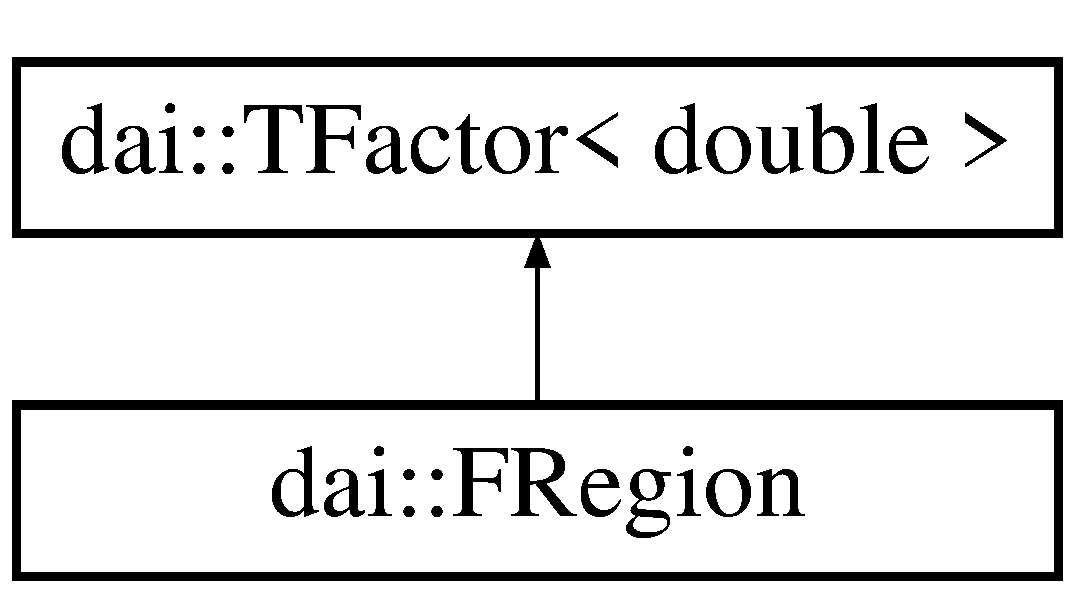
\includegraphics[height=2cm]{classdai_1_1FRegion}
\end{center}
\end{figure}


\subsection{Detailed Description}
A \hyperlink{classdai_1_1FRegion}{FRegion} is a factor with a counting number. \subsection*{Public Member Functions}
\begin{CompactItemize}
\item 
\hypertarget{classdai_1_1FRegion_b81b699de467dab74cd11d315497c636}{
\hyperlink{classdai_1_1FRegion_b81b699de467dab74cd11d315497c636}{FRegion} ()}
\label{classdai_1_1FRegion_b81b699de467dab74cd11d315497c636}

\begin{CompactList}\small\item\em Default constructor. \item\end{CompactList}\item 
\hypertarget{classdai_1_1FRegion_72b2f014dfb2f98aefa18f2972cf9108}{
\hyperlink{classdai_1_1FRegion_72b2f014dfb2f98aefa18f2972cf9108}{FRegion} (const \hyperlink{classdai_1_1TFactor}{Factor} \&x, double c)}
\label{classdai_1_1FRegion_72b2f014dfb2f98aefa18f2972cf9108}

\begin{CompactList}\small\item\em Constructs \hyperlink{classdai_1_1FRegion}{FRegion} from a Factor and a counting number. \item\end{CompactList}\item 
\hypertarget{classdai_1_1FRegion_ba8e41c104c66c0c6c47a12184b0df17}{
\hyperlink{classdai_1_1FRegion_ba8e41c104c66c0c6c47a12184b0df17}{FRegion} (const \hyperlink{classdai_1_1FRegion}{FRegion} \&x)}
\label{classdai_1_1FRegion_ba8e41c104c66c0c6c47a12184b0df17}

\begin{CompactList}\small\item\em Copy constructor. \item\end{CompactList}\item 
\hypertarget{classdai_1_1FRegion_2a6f340d8cfdef5e5925f5030160920d}{
\hyperlink{classdai_1_1FRegion}{FRegion} \& \hyperlink{classdai_1_1FRegion_2a6f340d8cfdef5e5925f5030160920d}{operator=} (const \hyperlink{classdai_1_1FRegion}{FRegion} \&x)}
\label{classdai_1_1FRegion_2a6f340d8cfdef5e5925f5030160920d}

\begin{CompactList}\small\item\em Assignment operator. \item\end{CompactList}\item 
\hypertarget{classdai_1_1FRegion_94c63ec48848b132eeb024515978f654}{
const double \& \hyperlink{classdai_1_1FRegion_94c63ec48848b132eeb024515978f654}{c} () const }
\label{classdai_1_1FRegion_94c63ec48848b132eeb024515978f654}

\begin{CompactList}\small\item\em Provide read access to counting number. \item\end{CompactList}\item 
\hypertarget{classdai_1_1FRegion_f6e5b1ea80c052f98056d29d47a76145}{
double \& \hyperlink{classdai_1_1FRegion_f6e5b1ea80c052f98056d29d47a76145}{c} ()}
\label{classdai_1_1FRegion_f6e5b1ea80c052f98056d29d47a76145}

\begin{CompactList}\small\item\em Provide full access to counting number. \item\end{CompactList}\item 
\hypertarget{classdai_1_1TFactor_c742180c0abe1be45fbf3208f7014a1b}{
const \hyperlink{classdai_1_1TProb}{TProb}$<$ T $>$ \& \hyperlink{classdai_1_1TFactor_c742180c0abe1be45fbf3208f7014a1b}{p} () const }
\label{classdai_1_1TFactor_c742180c0abe1be45fbf3208f7014a1b}

\begin{CompactList}\small\item\em Returns const reference to probability entries. \item\end{CompactList}\item 
\hypertarget{classdai_1_1TFactor_ba85b145db1c3b72978e11fb385659e1}{
\hyperlink{classdai_1_1TProb}{TProb}$<$ T $>$ \& \hyperlink{classdai_1_1TFactor_ba85b145db1c3b72978e11fb385659e1}{p} ()}
\label{classdai_1_1TFactor_ba85b145db1c3b72978e11fb385659e1}

\begin{CompactList}\small\item\em Returns reference to probability entries. \item\end{CompactList}\item 
\hypertarget{classdai_1_1TFactor_54c575d53b8c8a6a03c26c8cdc600ce4}{
const \hyperlink{classdai_1_1VarSet}{VarSet} \& \hyperlink{classdai_1_1TFactor_54c575d53b8c8a6a03c26c8cdc600ce4}{vars} () const }
\label{classdai_1_1TFactor_54c575d53b8c8a6a03c26c8cdc600ce4}

\begin{CompactList}\small\item\em Returns const reference to variables. \item\end{CompactList}\item 
\hypertarget{classdai_1_1TFactor_57d676927a5dcacbef47f564c46bf128}{
size\_\-t \hyperlink{classdai_1_1TFactor_57d676927a5dcacbef47f564c46bf128}{states} () const }
\label{classdai_1_1TFactor_57d676927a5dcacbef47f564c46bf128}

\begin{CompactList}\small\item\em Returns the number of possible joint states of the variables. \item\end{CompactList}\item 
\hypertarget{classdai_1_1TFactor_22a12143c01d05a1e70ca3f92ec42595}{
T \hyperlink{classdai_1_1TFactor_22a12143c01d05a1e70ca3f92ec42595}{operator\mbox{[}$\,$\mbox{]}} (size\_\-t i) const }
\label{classdai_1_1TFactor_22a12143c01d05a1e70ca3f92ec42595}

\begin{CompactList}\small\item\em Returns a copy of the i'th probability value. \item\end{CompactList}\item 
\hypertarget{classdai_1_1TFactor_8be917166f0f32f2da09e09fc5fa2651}{
T \& \hyperlink{classdai_1_1TFactor_8be917166f0f32f2da09e09fc5fa2651}{operator\mbox{[}$\,$\mbox{]}} (size\_\-t i)}
\label{classdai_1_1TFactor_8be917166f0f32f2da09e09fc5fa2651}

\begin{CompactList}\small\item\em Returns a reference to the i'th probability value. \item\end{CompactList}\item 
\hypertarget{classdai_1_1TFactor_949ed2c4aefdf1aadfe33d0c2dac89b3}{
\hyperlink{classdai_1_1TFactor}{TFactor}$<$ T $>$ \& \hyperlink{classdai_1_1TFactor_949ed2c4aefdf1aadfe33d0c2dac89b3}{fill} (T p)}
\label{classdai_1_1TFactor_949ed2c4aefdf1aadfe33d0c2dac89b3}

\begin{CompactList}\small\item\em Sets all probability entries to p. \item\end{CompactList}\item 
\hypertarget{classdai_1_1TFactor_f52a4ee1544b4e628390918239b7bc1b}{
\hyperlink{classdai_1_1TFactor}{TFactor}$<$ T $>$ \& \hyperlink{classdai_1_1TFactor_f52a4ee1544b4e628390918239b7bc1b}{randomize} ()}
\label{classdai_1_1TFactor_f52a4ee1544b4e628390918239b7bc1b}

\begin{CompactList}\small\item\em Fills all probability entries with random values. \item\end{CompactList}\item 
\hypertarget{classdai_1_1TFactor_cf5fc0dd70aa8a7e7c2da3b3acdf6747}{
\hyperlink{classdai_1_1TFactor}{TFactor}$<$ T $>$ \hyperlink{classdai_1_1TFactor_cf5fc0dd70aa8a7e7c2da3b3acdf6747}{operator$\ast$} (T x) const }
\label{classdai_1_1TFactor_cf5fc0dd70aa8a7e7c2da3b3acdf6747}

\begin{CompactList}\small\item\em Returns product of $\ast$this with x. \item\end{CompactList}\item 
\hypertarget{classdai_1_1TFactor_53f052f85f5274b783eaa1ecd31a6b35}{
\hyperlink{classdai_1_1TFactor}{TFactor}$<$ T $>$ \hyperlink{classdai_1_1TFactor_53f052f85f5274b783eaa1ecd31a6b35}{operator$\ast$} (const \hyperlink{classdai_1_1TFactor}{TFactor}$<$ T $>$ \&Q) const }
\label{classdai_1_1TFactor_53f052f85f5274b783eaa1ecd31a6b35}

\begin{CompactList}\small\item\em Returns product of $\ast$this with another Factor. \item\end{CompactList}\item 
\hypertarget{classdai_1_1TFactor_e8a33191e3bc570737ff29e77966c33e}{
\hyperlink{classdai_1_1TFactor}{TFactor}$<$ T $>$ \& \hyperlink{classdai_1_1TFactor_e8a33191e3bc570737ff29e77966c33e}{operator$\ast$=} (T x)}
\label{classdai_1_1TFactor_e8a33191e3bc570737ff29e77966c33e}

\begin{CompactList}\small\item\em Multiplies each probability entry with x. \item\end{CompactList}\item 
\hypertarget{classdai_1_1TFactor_914cb4b11fdffa4daaebf645f539d5d1}{
\hyperlink{classdai_1_1TFactor}{TFactor}$<$ T $>$ \& \hyperlink{classdai_1_1TFactor_914cb4b11fdffa4daaebf645f539d5d1}{operator$\ast$=} (const \hyperlink{classdai_1_1TFactor}{TFactor}$<$ T $>$ \&Q)}
\label{classdai_1_1TFactor_914cb4b11fdffa4daaebf645f539d5d1}

\begin{CompactList}\small\item\em Multiplies $\ast$this with another Factor. \item\end{CompactList}\item 
\hypertarget{classdai_1_1TFactor_35fd7313a64a83aba0cd087d1b60289d}{
\hyperlink{classdai_1_1TFactor}{TFactor}$<$ T $>$ \hyperlink{classdai_1_1TFactor_35fd7313a64a83aba0cd087d1b60289d}{operator/} (T x) const }
\label{classdai_1_1TFactor_35fd7313a64a83aba0cd087d1b60289d}

\begin{CompactList}\small\item\em Returns quotient of $\ast$this with x. \item\end{CompactList}\item 
\hypertarget{classdai_1_1TFactor_f5894eb556d2c440774e650102207d80}{
\hyperlink{classdai_1_1TFactor}{TFactor}$<$ T $>$ \hyperlink{classdai_1_1TFactor_f5894eb556d2c440774e650102207d80}{operator/} (const \hyperlink{classdai_1_1TFactor}{TFactor}$<$ T $>$ \&Q) const }
\label{classdai_1_1TFactor_f5894eb556d2c440774e650102207d80}

\begin{CompactList}\small\item\em Returns quotient of $\ast$this with another Factor. \item\end{CompactList}\item 
\hypertarget{classdai_1_1TFactor_45c34bf15cc9b37e5c0718d96d9d2c1a}{
\hyperlink{classdai_1_1TFactor}{TFactor}$<$ T $>$ \& \hyperlink{classdai_1_1TFactor_45c34bf15cc9b37e5c0718d96d9d2c1a}{operator/=} (T x)}
\label{classdai_1_1TFactor_45c34bf15cc9b37e5c0718d96d9d2c1a}

\begin{CompactList}\small\item\em Divides each probability entry by x. \item\end{CompactList}\item 
\hypertarget{classdai_1_1TFactor_c5ac7c898b536ecbed7a1f58e3899cdb}{
\hyperlink{classdai_1_1TFactor}{TFactor}$<$ T $>$ \& \hyperlink{classdai_1_1TFactor_c5ac7c898b536ecbed7a1f58e3899cdb}{operator/=} (const \hyperlink{classdai_1_1TFactor}{TFactor}$<$ T $>$ \&Q)}
\label{classdai_1_1TFactor_c5ac7c898b536ecbed7a1f58e3899cdb}

\begin{CompactList}\small\item\em Divides $\ast$this by another Factor. \item\end{CompactList}\item 
\hypertarget{classdai_1_1TFactor_5db00c03b427e577bab01646c451ae23}{
\hyperlink{classdai_1_1TFactor}{TFactor}$<$ T $>$ \hyperlink{classdai_1_1TFactor_5db00c03b427e577bab01646c451ae23}{operator+} (const \hyperlink{classdai_1_1TFactor}{TFactor}$<$ T $>$ \&Q) const }
\label{classdai_1_1TFactor_5db00c03b427e577bab01646c451ae23}

\begin{CompactList}\small\item\em Returns sum of $\ast$this and another Factor (their \hyperlink{classdai_1_1TFactor_54c575d53b8c8a6a03c26c8cdc600ce4}{vars()} should be identical). \item\end{CompactList}\item 
\hypertarget{classdai_1_1TFactor_3c2f95c6fddf19bd871a89f419991c08}{
\hyperlink{classdai_1_1TFactor}{TFactor}$<$ T $>$ \hyperlink{classdai_1_1TFactor_3c2f95c6fddf19bd871a89f419991c08}{operator+} (T q) const }
\label{classdai_1_1TFactor_3c2f95c6fddf19bd871a89f419991c08}

\begin{CompactList}\small\item\em Returns sum of $\ast$this and a scalar. \item\end{CompactList}\item 
\hypertarget{classdai_1_1TFactor_36cd699efe9bcce52fb21d6a3eb7024a}{
\hyperlink{classdai_1_1TFactor}{TFactor}$<$ T $>$ \hyperlink{classdai_1_1TFactor_36cd699efe9bcce52fb21d6a3eb7024a}{operator-} (const \hyperlink{classdai_1_1TFactor}{TFactor}$<$ T $>$ \&Q) const }
\label{classdai_1_1TFactor_36cd699efe9bcce52fb21d6a3eb7024a}

\begin{CompactList}\small\item\em Returns difference of $\ast$this and another Factor (their \hyperlink{classdai_1_1TFactor_54c575d53b8c8a6a03c26c8cdc600ce4}{vars()} should be identical). \item\end{CompactList}\item 
\hypertarget{classdai_1_1TFactor_171e3bab13b2cd054e8ce1eb97be1112}{
\hyperlink{classdai_1_1TFactor}{TFactor}$<$ T $>$ \hyperlink{classdai_1_1TFactor_171e3bab13b2cd054e8ce1eb97be1112}{operator-} (T q) const }
\label{classdai_1_1TFactor_171e3bab13b2cd054e8ce1eb97be1112}

\begin{CompactList}\small\item\em Returns difference of $\ast$this with a scalar. \item\end{CompactList}\item 
\hypertarget{classdai_1_1TFactor_098a7c22159f23dead9e16ad3dff1e90}{
\hyperlink{classdai_1_1TFactor}{TFactor}$<$ T $>$ \& \hyperlink{classdai_1_1TFactor_098a7c22159f23dead9e16ad3dff1e90}{operator+=} (const \hyperlink{classdai_1_1TFactor}{TFactor}$<$ T $>$ \&Q)}
\label{classdai_1_1TFactor_098a7c22159f23dead9e16ad3dff1e90}

\begin{CompactList}\small\item\em Adds another Factor to $\ast$this (their \hyperlink{classdai_1_1TFactor_54c575d53b8c8a6a03c26c8cdc600ce4}{vars()} should be identical). \item\end{CompactList}\item 
\hypertarget{classdai_1_1TFactor_fda1418de5d67a6ba004eaea3ef66f77}{
\hyperlink{classdai_1_1TFactor}{TFactor}$<$ T $>$ \& \hyperlink{classdai_1_1TFactor_fda1418de5d67a6ba004eaea3ef66f77}{operator+=} (T q)}
\label{classdai_1_1TFactor_fda1418de5d67a6ba004eaea3ef66f77}

\begin{CompactList}\small\item\em Adds scalar to $\ast$this. \item\end{CompactList}\item 
\hypertarget{classdai_1_1TFactor_a6dd7ae3384f6f329e2cb3c3fa31e514}{
\hyperlink{classdai_1_1TFactor}{TFactor}$<$ T $>$ \& \hyperlink{classdai_1_1TFactor_a6dd7ae3384f6f329e2cb3c3fa31e514}{operator-=} (const \hyperlink{classdai_1_1TFactor}{TFactor}$<$ T $>$ \&Q)}
\label{classdai_1_1TFactor_a6dd7ae3384f6f329e2cb3c3fa31e514}

\begin{CompactList}\small\item\em Subtracts another Factor from $\ast$this (their \hyperlink{classdai_1_1TFactor_54c575d53b8c8a6a03c26c8cdc600ce4}{vars()} should be identical). \item\end{CompactList}\item 
\hypertarget{classdai_1_1TFactor_d74386483d4f28011ddc962db443e3aa}{
\hyperlink{classdai_1_1TFactor}{TFactor}$<$ T $>$ \& \hyperlink{classdai_1_1TFactor_d74386483d4f28011ddc962db443e3aa}{operator-=} (T q)}
\label{classdai_1_1TFactor_d74386483d4f28011ddc962db443e3aa}

\begin{CompactList}\small\item\em Subtracts scalar from $\ast$this. \item\end{CompactList}\item 
\hypertarget{classdai_1_1TFactor_9b87c70ab153534d5cdbbdba6aaa7921}{
\hyperlink{classdai_1_1TFactor}{TFactor}$<$ T $>$ \hyperlink{classdai_1_1TFactor_9b87c70ab153534d5cdbbdba6aaa7921}{operator$^\wedge$} (\hyperlink{namespacedai_e7d0472fdc89a8635825d01940e91cbf}{Real} a) const }
\label{classdai_1_1TFactor_9b87c70ab153534d5cdbbdba6aaa7921}

\begin{CompactList}\small\item\em Returns $\ast$this raised to some power. \item\end{CompactList}\item 
\hypertarget{classdai_1_1TFactor_4cd8337eb9ae63205692a28435322d3b}{
\hyperlink{classdai_1_1TFactor}{TFactor}$<$ T $>$ \& \hyperlink{classdai_1_1TFactor_4cd8337eb9ae63205692a28435322d3b}{operator$^\wedge$=} (\hyperlink{namespacedai_e7d0472fdc89a8635825d01940e91cbf}{Real} a)}
\label{classdai_1_1TFactor_4cd8337eb9ae63205692a28435322d3b}

\begin{CompactList}\small\item\em Raises $\ast$this to some power. \item\end{CompactList}\item 
\hypertarget{classdai_1_1TFactor_8ab0a98ebf512cd5a27e6a2618ed4353}{
\hyperlink{classdai_1_1TFactor}{TFactor}$<$ T $>$ \& \hyperlink{classdai_1_1TFactor_8ab0a98ebf512cd5a27e6a2618ed4353}{makeZero} (\hyperlink{namespacedai_e7d0472fdc89a8635825d01940e91cbf}{Real} epsilon)}
\label{classdai_1_1TFactor_8ab0a98ebf512cd5a27e6a2618ed4353}

\begin{CompactList}\small\item\em Sets all entries that are smaller than epsilon to zero. \item\end{CompactList}\item 
\hypertarget{classdai_1_1TFactor_731c8683fc17269c4bf3f7b52e0c4b40}{
\hyperlink{classdai_1_1TFactor}{TFactor}$<$ T $>$ \& \hyperlink{classdai_1_1TFactor_731c8683fc17269c4bf3f7b52e0c4b40}{makePositive} (\hyperlink{namespacedai_e7d0472fdc89a8635825d01940e91cbf}{Real} epsilon)}
\label{classdai_1_1TFactor_731c8683fc17269c4bf3f7b52e0c4b40}

\begin{CompactList}\small\item\em Sets all entries that are smaller than epsilon to epsilon. \item\end{CompactList}\item 
\hypertarget{classdai_1_1TFactor_de249c30222894e50170a834aca6d708}{
\hyperlink{classdai_1_1TFactor}{TFactor}$<$ T $>$ \hyperlink{classdai_1_1TFactor_de249c30222894e50170a834aca6d708}{inverse} () const }
\label{classdai_1_1TFactor_de249c30222894e50170a834aca6d708}

\begin{CompactList}\small\item\em Returns inverse of $\ast$this. \item\end{CompactList}\item 
\hypertarget{classdai_1_1TFactor_1747eaa67d359d34d9221d368753ecdf}{
\hyperlink{classdai_1_1TFactor}{TFactor}$<$ T $>$ \hyperlink{classdai_1_1TFactor_1747eaa67d359d34d9221d368753ecdf}{divided\_\-by} (const \hyperlink{classdai_1_1TFactor}{TFactor}$<$ T $>$ \&denom) const }
\label{classdai_1_1TFactor_1747eaa67d359d34d9221d368753ecdf}

\begin{CompactList}\small\item\em Returns $\ast$this divided by another Factor. \item\end{CompactList}\item 
\hypertarget{classdai_1_1TFactor_275c1fd149c36a9e67256d21ad97dde1}{
\hyperlink{classdai_1_1TFactor}{TFactor}$<$ T $>$ \& \hyperlink{classdai_1_1TFactor_275c1fd149c36a9e67256d21ad97dde1}{divide} (const \hyperlink{classdai_1_1TFactor}{TFactor}$<$ T $>$ \&denom)}
\label{classdai_1_1TFactor_275c1fd149c36a9e67256d21ad97dde1}

\begin{CompactList}\small\item\em Divides $\ast$this by another Factor. \item\end{CompactList}\item 
\hypertarget{classdai_1_1TFactor_284a962817d33244c261be5d7f0159ca}{
\hyperlink{classdai_1_1TFactor}{TFactor}$<$ T $>$ \hyperlink{classdai_1_1TFactor_284a962817d33244c261be5d7f0159ca}{exp} () const }
\label{classdai_1_1TFactor_284a962817d33244c261be5d7f0159ca}

\begin{CompactList}\small\item\em Returns exp of $\ast$this. \item\end{CompactList}\item 
\hypertarget{classdai_1_1TFactor_fa3435d85ca11399aba42c63a008765a}{
\hyperlink{classdai_1_1TFactor}{TFactor}$<$ T $>$ \hyperlink{classdai_1_1TFactor_fa3435d85ca11399aba42c63a008765a}{abs} () const }
\label{classdai_1_1TFactor_fa3435d85ca11399aba42c63a008765a}

\begin{CompactList}\small\item\em Returns absolute value of $\ast$this. \item\end{CompactList}\item 
\hypertarget{classdai_1_1TFactor_fbbcf3a69afa5fb3bde1f5a8180860c6}{
\hyperlink{classdai_1_1TFactor}{TFactor}$<$ T $>$ \hyperlink{classdai_1_1TFactor_fbbcf3a69afa5fb3bde1f5a8180860c6}{log} () const }
\label{classdai_1_1TFactor_fbbcf3a69afa5fb3bde1f5a8180860c6}

\begin{CompactList}\small\item\em Returns logarithm of $\ast$this. \item\end{CompactList}\item 
\hypertarget{classdai_1_1TFactor_72b37d26ccac6edb39e71209bb675ba7}{
\hyperlink{classdai_1_1TFactor}{TFactor}$<$ T $>$ \hyperlink{classdai_1_1TFactor_72b37d26ccac6edb39e71209bb675ba7}{log0} () const }
\label{classdai_1_1TFactor_72b37d26ccac6edb39e71209bb675ba7}

\begin{CompactList}\small\item\em Returns logarithm of $\ast$this (defining log(0)=0). \item\end{CompactList}\item 
\hypertarget{classdai_1_1TFactor_c69a94a4d055c3cac107b2a55bb42944}{
T \hyperlink{classdai_1_1TFactor_c69a94a4d055c3cac107b2a55bb42944}{normalize} (typename \hyperlink{classdai_1_1TProb_31d9206096f52574dbd24cbb2502080c}{Prob::NormType} norm=Prob::NORMPROB)}
\label{classdai_1_1TFactor_c69a94a4d055c3cac107b2a55bb42944}

\begin{CompactList}\small\item\em Normalizes $\ast$this Factor. \item\end{CompactList}\item 
\hypertarget{classdai_1_1TFactor_df4740f4558ed9bc27029c0c362923e2}{
\hyperlink{classdai_1_1TFactor}{TFactor}$<$ T $>$ \hyperlink{classdai_1_1TFactor_df4740f4558ed9bc27029c0c362923e2}{normalized} (typename \hyperlink{classdai_1_1TProb_31d9206096f52574dbd24cbb2502080c}{Prob::NormType} norm=Prob::NORMPROB) const }
\label{classdai_1_1TFactor_df4740f4558ed9bc27029c0c362923e2}

\begin{CompactList}\small\item\em Returns a normalized copy of $\ast$this. \item\end{CompactList}\item 
\hypertarget{classdai_1_1TFactor_7cc9e6bca2b9c187f8d907942264508f}{
\hyperlink{classdai_1_1TFactor}{Factor} \hyperlink{classdai_1_1TFactor_7cc9e6bca2b9c187f8d907942264508f}{slice} (const \hyperlink{classdai_1_1VarSet}{VarSet} \&ns, size\_\-t ns\_\-state) const }
\label{classdai_1_1TFactor_7cc9e6bca2b9c187f8d907942264508f}

\begin{CompactList}\small\item\em Returns a slice of this factor, where the subset ns is in state ns\_\-state. \item\end{CompactList}\item 
\hypertarget{classdai_1_1TFactor_f90e2a8a5ef94809ae8905e19fc523e4}{
\hyperlink{classdai_1_1TFactor}{TFactor}$<$ T $>$ \hyperlink{classdai_1_1TFactor_f90e2a8a5ef94809ae8905e19fc523e4}{partSum} (const \hyperlink{classdai_1_1VarSet}{VarSet} \&ns) const }
\label{classdai_1_1TFactor_f90e2a8a5ef94809ae8905e19fc523e4}

\begin{CompactList}\small\item\em Returns unnormalized marginal; ns should be a subset of \hyperlink{classdai_1_1TFactor_54c575d53b8c8a6a03c26c8cdc600ce4}{vars()}. \item\end{CompactList}\item 
\hypertarget{classdai_1_1TFactor_692df5b8aed5f6faeb60e076624d5854}{
\hyperlink{classdai_1_1TFactor}{TFactor}$<$ T $>$ \hyperlink{classdai_1_1TFactor_692df5b8aed5f6faeb60e076624d5854}{marginal} (const \hyperlink{classdai_1_1VarSet}{VarSet} \&ns, bool normed=true) const }
\label{classdai_1_1TFactor_692df5b8aed5f6faeb60e076624d5854}

\begin{CompactList}\small\item\em Returns (normalized by default) marginal; ns should be a subset of \hyperlink{classdai_1_1TFactor_54c575d53b8c8a6a03c26c8cdc600ce4}{vars()}. \item\end{CompactList}\item 
\hypertarget{classdai_1_1TFactor_fd92183f10a4214341ce771b02f8744d}{
\hyperlink{classdai_1_1TFactor}{TFactor}$<$ T $>$ \hyperlink{classdai_1_1TFactor_fd92183f10a4214341ce771b02f8744d}{notSum} (const \hyperlink{classdai_1_1VarSet}{VarSet} \&ns) const }
\label{classdai_1_1TFactor_fd92183f10a4214341ce771b02f8744d}

\begin{CompactList}\small\item\em Sums out all variables except those in ns. \item\end{CompactList}\item 
\hypertarget{classdai_1_1TFactor_81c344b9e204bb57aaca92c281aa7dd3}{
\hyperlink{classdai_1_1TFactor}{TFactor}$<$ T $>$ \hyperlink{classdai_1_1TFactor_81c344b9e204bb57aaca92c281aa7dd3}{embed} (const \hyperlink{classdai_1_1VarSet}{VarSet} \&ns) const }
\label{classdai_1_1TFactor_81c344b9e204bb57aaca92c281aa7dd3}

\begin{CompactList}\small\item\em Embeds this factor in a larger \hyperlink{classdai_1_1VarSet}{VarSet}. \item\end{CompactList}\item 
\hypertarget{classdai_1_1TFactor_dafb816c6d9f93ceea858709391841d2}{
bool \hyperlink{classdai_1_1TFactor_dafb816c6d9f93ceea858709391841d2}{hasNaNs} () const }
\label{classdai_1_1TFactor_dafb816c6d9f93ceea858709391841d2}

\begin{CompactList}\small\item\em Returns true if $\ast$this has NANs. \item\end{CompactList}\item 
\hypertarget{classdai_1_1TFactor_7353d87f8a1d4c6c24b9cc5de7b18219}{
bool \hyperlink{classdai_1_1TFactor_7353d87f8a1d4c6c24b9cc5de7b18219}{hasNegatives} () const }
\label{classdai_1_1TFactor_7353d87f8a1d4c6c24b9cc5de7b18219}

\begin{CompactList}\small\item\em Returns true if $\ast$this has negative entries. \item\end{CompactList}\item 
\hypertarget{classdai_1_1TFactor_aff9f62e6ef5792a459946cd81bd35af}{
T \hyperlink{classdai_1_1TFactor_aff9f62e6ef5792a459946cd81bd35af}{totalSum} () const }
\label{classdai_1_1TFactor_aff9f62e6ef5792a459946cd81bd35af}

\begin{CompactList}\small\item\em Returns total sum of probability entries. \item\end{CompactList}\item 
\hypertarget{classdai_1_1TFactor_8e67b044dfaebf20c77031a2378e65f5}{
T \hyperlink{classdai_1_1TFactor_8e67b044dfaebf20c77031a2378e65f5}{maxAbs} () const }
\label{classdai_1_1TFactor_8e67b044dfaebf20c77031a2378e65f5}

\begin{CompactList}\small\item\em Returns maximum absolute value of probability entries. \item\end{CompactList}\item 
\hypertarget{classdai_1_1TFactor_160c82f59a3202180025853a9e5caaa5}{
T \hyperlink{classdai_1_1TFactor_160c82f59a3202180025853a9e5caaa5}{maxVal} () const }
\label{classdai_1_1TFactor_160c82f59a3202180025853a9e5caaa5}

\begin{CompactList}\small\item\em Returns maximum value of probability entries. \item\end{CompactList}\item 
\hypertarget{classdai_1_1TFactor_891e98fd0cd9f65f945eb5733c6c3e9f}{
T \hyperlink{classdai_1_1TFactor_891e98fd0cd9f65f945eb5733c6c3e9f}{minVal} () const }
\label{classdai_1_1TFactor_891e98fd0cd9f65f945eb5733c6c3e9f}

\begin{CompactList}\small\item\em Returns minimum value of probability entries. \item\end{CompactList}\item 
\hypertarget{classdai_1_1TFactor_948c0013f741040ecdcad7da53377268}{
\hyperlink{namespacedai_e7d0472fdc89a8635825d01940e91cbf}{Real} \hyperlink{classdai_1_1TFactor_948c0013f741040ecdcad7da53377268}{entropy} () const }
\label{classdai_1_1TFactor_948c0013f741040ecdcad7da53377268}

\begin{CompactList}\small\item\em Returns entropy of $\ast$this. \item\end{CompactList}\item 
\hypertarget{classdai_1_1TFactor_4908ad29222b60d669d234d0805605b8}{
T \hyperlink{classdai_1_1TFactor_4908ad29222b60d669d234d0805605b8}{strength} (const \hyperlink{classdai_1_1Var}{Var} \&i, const \hyperlink{classdai_1_1Var}{Var} \&j) const }
\label{classdai_1_1TFactor_4908ad29222b60d669d234d0805605b8}

\begin{CompactList}\small\item\em Returns strength of $\ast$this, between variables i and j, using (52) of \mbox{[}\hyperlink{Bibliography_MoK07b}{MoK07b}\mbox{]}. \item\end{CompactList}\end{CompactItemize}


The documentation for this class was generated from the following file:\begin{CompactItemize}
\item 
include/dai/\hyperlink{regiongraph_8h}{regiongraph.h}\end{CompactItemize}

\hypertarget{classdai_1_1HAK}{
\section{dai::HAK Class Reference}
\label{classdai_1_1HAK}\index{dai::HAK@{dai::HAK}}
}
{\tt \#include $<$dai/hak.h$>$}

Inheritance diagram for dai::HAK::\begin{figure}[H]
\begin{center}
\leavevmode
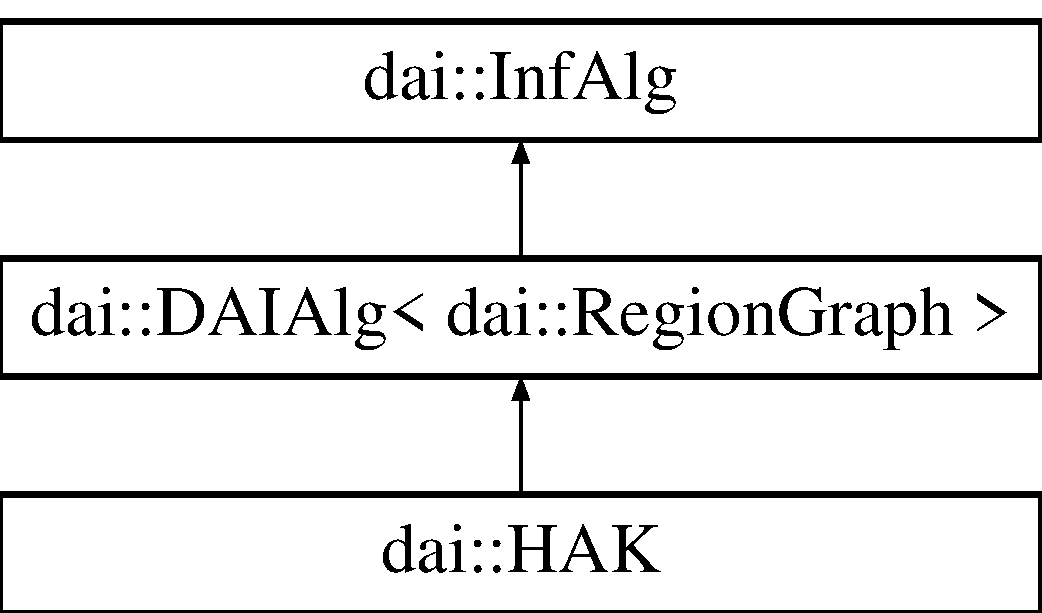
\includegraphics[height=3cm]{classdai_1_1HAK}
\end{center}
\end{figure}


\subsection{Detailed Description}
Approximate inference algorithm: implementation of single-loop (\char`\"{}Generalized Belief Propagation\char`\"{}) and double-loop algorithms by Heskes, Albers and Kappen. \subsection*{Public Member Functions}
\begin{CompactItemize}
\item 
\hypertarget{classdai_1_1HAK_deffdd4894e50b585d11cab9e9813d6f}{
\hyperlink{classdai_1_1HAK_deffdd4894e50b585d11cab9e9813d6f}{HAK} ()}
\label{classdai_1_1HAK_deffdd4894e50b585d11cab9e9813d6f}

\begin{CompactList}\small\item\em Default constructor. \item\end{CompactList}\item 
\hypertarget{classdai_1_1HAK_d956a4113227fae22e2c5c30ee003622}{
\hyperlink{classdai_1_1HAK_d956a4113227fae22e2c5c30ee003622}{HAK} (const \hyperlink{classdai_1_1HAK}{HAK} \&x)}
\label{classdai_1_1HAK_d956a4113227fae22e2c5c30ee003622}

\begin{CompactList}\small\item\em Copy constructor. \item\end{CompactList}\item 
\hypertarget{classdai_1_1HAK_ee00f8b04cc05ef8516800d4ec56b7b4}{
\hyperlink{classdai_1_1HAK}{HAK} \& \hyperlink{classdai_1_1HAK_ee00f8b04cc05ef8516800d4ec56b7b4}{operator=} (const \hyperlink{classdai_1_1HAK}{HAK} \&x)}
\label{classdai_1_1HAK_ee00f8b04cc05ef8516800d4ec56b7b4}

\begin{CompactList}\small\item\em Assignment operator. \item\end{CompactList}\item 
\hypertarget{classdai_1_1HAK_5cd7000971e68e732d5dffa7c665804a}{
\hyperlink{classdai_1_1HAK_5cd7000971e68e732d5dffa7c665804a}{HAK} (const \hyperlink{classdai_1_1FactorGraph}{FactorGraph} \&fg, const \hyperlink{classdai_1_1PropertySet}{PropertySet} \&opts)}
\label{classdai_1_1HAK_5cd7000971e68e732d5dffa7c665804a}

\begin{CompactList}\small\item\em Construct from \hyperlink{classdai_1_1FactorGraph}{FactorGraph} fg and \hyperlink{classdai_1_1PropertySet}{PropertySet} opts. \item\end{CompactList}\item 
\hypertarget{classdai_1_1HAK_f0608983940f78bd6fefe0933404861e}{
\hyperlink{classdai_1_1HAK_f0608983940f78bd6fefe0933404861e}{HAK} (const \hyperlink{classdai_1_1RegionGraph}{RegionGraph} \&rg, const \hyperlink{classdai_1_1PropertySet}{PropertySet} \&opts)}
\label{classdai_1_1HAK_f0608983940f78bd6fefe0933404861e}

\begin{CompactList}\small\item\em Construct from \hyperlink{classdai_1_1RegionGraph}{RegionGraph} rg and \hyperlink{classdai_1_1PropertySet}{PropertySet} opts. \item\end{CompactList}\item 
\hypertarget{classdai_1_1DAIAlg_48ba6a58d10b8802d690e5e92ec5abe9}{
void \hyperlink{classdai_1_1DAIAlg_48ba6a58d10b8802d690e5e92ec5abe9}{backupFactor} (size\_\-t I)}
\label{classdai_1_1DAIAlg_48ba6a58d10b8802d690e5e92ec5abe9}

\begin{CompactList}\small\item\em Save factor I. \item\end{CompactList}\item 
\hypertarget{classdai_1_1DAIAlg_0176904d3b4b9d083288ea8c4a2dc8bc}{
void \hyperlink{classdai_1_1DAIAlg_0176904d3b4b9d083288ea8c4a2dc8bc}{backupFactors} (const \hyperlink{classdai_1_1VarSet}{VarSet} \&ns)}
\label{classdai_1_1DAIAlg_0176904d3b4b9d083288ea8c4a2dc8bc}

\begin{CompactList}\small\item\em Save Factors involving ns. \item\end{CompactList}\item 
\hypertarget{classdai_1_1DAIAlg_bf8dbd2797ec871e86566a6dfc0864e3}{
void \hyperlink{classdai_1_1DAIAlg_bf8dbd2797ec871e86566a6dfc0864e3}{restoreFactor} (size\_\-t I)}
\label{classdai_1_1DAIAlg_bf8dbd2797ec871e86566a6dfc0864e3}

\begin{CompactList}\small\item\em Restore factor I. \item\end{CompactList}\item 
\hypertarget{classdai_1_1DAIAlg_3ce97e9370f1cdc785526c1a6c1eaadf}{
void \hyperlink{classdai_1_1DAIAlg_3ce97e9370f1cdc785526c1a6c1eaadf}{restoreFactors} (const \hyperlink{classdai_1_1VarSet}{VarSet} \&ns)}
\label{classdai_1_1DAIAlg_3ce97e9370f1cdc785526c1a6c1eaadf}

\begin{CompactList}\small\item\em Restore Factors involving ns. \item\end{CompactList}\item 
\hypertarget{classdai_1_1DAIAlg_b7d537f1a9d116617d8dce722ce65dc0}{
void \hyperlink{classdai_1_1DAIAlg_b7d537f1a9d116617d8dce722ce65dc0}{clamp} (const \hyperlink{classdai_1_1Var}{Var} \&n, size\_\-t i, bool backup=false)}
\label{classdai_1_1DAIAlg_b7d537f1a9d116617d8dce722ce65dc0}

\begin{CompactList}\small\item\em Clamp variable n to value i (i.e. multiply with a Kronecker delta $\delta_{x_n, i}$). \item\end{CompactList}\item 
\hypertarget{classdai_1_1DAIAlg_7f0b8452352080a1e35ab9a68cb589fd}{
void \hyperlink{classdai_1_1DAIAlg_7f0b8452352080a1e35ab9a68cb589fd}{makeCavity} (size\_\-t i, bool backup=false)}
\label{classdai_1_1DAIAlg_7f0b8452352080a1e35ab9a68cb589fd}

\begin{CompactList}\small\item\em Set all factors interacting with var(i) to 1. \item\end{CompactList}\item 
\hypertarget{classdai_1_1DAIAlg_9348542c22d04ed804388f1fe3009fa3}{
\hyperlink{classdai_1_1FactorGraph}{FactorGraph} \& \hyperlink{classdai_1_1DAIAlg_9348542c22d04ed804388f1fe3009fa3}{fg} ()}
\label{classdai_1_1DAIAlg_9348542c22d04ed804388f1fe3009fa3}

\begin{CompactList}\small\item\em Get reference to underlying \hyperlink{classdai_1_1FactorGraph}{FactorGraph}. \item\end{CompactList}\item 
\hypertarget{classdai_1_1DAIAlg_35400e471b8c3c98bef6c74ceac8fa16}{
const \hyperlink{classdai_1_1FactorGraph}{FactorGraph} \& \hyperlink{classdai_1_1DAIAlg_35400e471b8c3c98bef6c74ceac8fa16}{fg} () const }
\label{classdai_1_1DAIAlg_35400e471b8c3c98bef6c74ceac8fa16}

\begin{CompactList}\small\item\em Get const reference to underlying \hyperlink{classdai_1_1FactorGraph}{FactorGraph}. \item\end{CompactList}\end{CompactItemize}
\begin{Indent}{\bf General InfAlg interface}\par
\begin{CompactItemize}
\item 
\hypertarget{classdai_1_1HAK_d128f5829b28e44aafcb9a4aae6881df}{
virtual \hyperlink{classdai_1_1HAK}{HAK} $\ast$ \hyperlink{classdai_1_1HAK_d128f5829b28e44aafcb9a4aae6881df}{clone} () const }
\label{classdai_1_1HAK_d128f5829b28e44aafcb9a4aae6881df}

\begin{CompactList}\small\item\em Returns a pointer to a new, cloned copy of $\ast$this (i.e., virtual copy constructor). \item\end{CompactList}\item 
\hypertarget{classdai_1_1HAK_895c9278a3958a7ad390c714386b0224}{
virtual \hyperlink{classdai_1_1HAK}{HAK} $\ast$ \hyperlink{classdai_1_1HAK_895c9278a3958a7ad390c714386b0224}{create} () const }
\label{classdai_1_1HAK_895c9278a3958a7ad390c714386b0224}

\begin{CompactList}\small\item\em Returns a pointer to a newly constructed object $\ast$this (i.e., virtual default constructor). \item\end{CompactList}\item 
\hypertarget{classdai_1_1HAK_05b7d9c9850ea10299b3dbce1e61bc23}{
virtual std::string \hyperlink{classdai_1_1HAK_05b7d9c9850ea10299b3dbce1e61bc23}{identify} () const }
\label{classdai_1_1HAK_05b7d9c9850ea10299b3dbce1e61bc23}

\begin{CompactList}\small\item\em Identifies itself for logging purposes. \item\end{CompactList}\item 
\hypertarget{classdai_1_1HAK_a08448a7be322c657568996d045d5b89}{
virtual \hyperlink{classdai_1_1TFactor}{Factor} \hyperlink{classdai_1_1HAK_a08448a7be322c657568996d045d5b89}{belief} (const \hyperlink{classdai_1_1Var}{Var} \&n) const }
\label{classdai_1_1HAK_a08448a7be322c657568996d045d5b89}

\begin{CompactList}\small\item\em Returns the \char`\"{}belief\char`\"{} (i.e., approximate marginal probability distribution) of a variable. \item\end{CompactList}\item 
\hypertarget{classdai_1_1HAK_c50b3b1bd84f2a8b9ea3b2ffab987f06}{
virtual \hyperlink{classdai_1_1TFactor}{Factor} \hyperlink{classdai_1_1HAK_c50b3b1bd84f2a8b9ea3b2ffab987f06}{belief} (const \hyperlink{classdai_1_1VarSet}{VarSet} \&ns) const }
\label{classdai_1_1HAK_c50b3b1bd84f2a8b9ea3b2ffab987f06}

\begin{CompactList}\small\item\em Returns the \char`\"{}belief\char`\"{} (i.e., approximate marginal probability distribution) of a set of variables. \item\end{CompactList}\item 
\hypertarget{classdai_1_1HAK_b0580070bad1f55d8d00c5e9c3c90e42}{
virtual std::vector$<$ \hyperlink{classdai_1_1TFactor}{Factor} $>$ \hyperlink{classdai_1_1HAK_b0580070bad1f55d8d00c5e9c3c90e42}{beliefs} () const }
\label{classdai_1_1HAK_b0580070bad1f55d8d00c5e9c3c90e42}

\begin{CompactList}\small\item\em Returns all \char`\"{}beliefs\char`\"{} (i.e., approximate marginal probability distribution) calculated by the algorithm. \item\end{CompactList}\item 
\hypertarget{classdai_1_1HAK_c1787a35ebd8c1cd1e615f4db00b828f}{
virtual \hyperlink{namespacedai_e7d0472fdc89a8635825d01940e91cbf}{Real} \hyperlink{classdai_1_1HAK_c1787a35ebd8c1cd1e615f4db00b828f}{logZ} () const }
\label{classdai_1_1HAK_c1787a35ebd8c1cd1e615f4db00b828f}

\begin{CompactList}\small\item\em Returns the logarithm of the (approximated) partition sum (normalizing constant of the factor graph). \item\end{CompactList}\item 
virtual void \hyperlink{classdai_1_1HAK_b30055f32f2c9a84d76668ff74606697}{init} ()
\begin{CompactList}\small\item\em Initializes all data structures of the approximate inference algorithm. \item\end{CompactList}\item 
virtual void \hyperlink{classdai_1_1HAK_53cd01bc1e70859d556ac71b5e25a192}{init} (const \hyperlink{classdai_1_1VarSet}{VarSet} \&ns)
\begin{CompactList}\small\item\em Initializes all data structures corresponding to some set of variables. \item\end{CompactList}\item 
\hypertarget{classdai_1_1HAK_0f9bade51e38b8fb955b7a61f88ecf20}{
virtual double \hyperlink{classdai_1_1HAK_0f9bade51e38b8fb955b7a61f88ecf20}{run} ()}
\label{classdai_1_1HAK_0f9bade51e38b8fb955b7a61f88ecf20}

\begin{CompactList}\small\item\em Runs the approximate inference algorithm. \item\end{CompactList}\item 
virtual double \hyperlink{classdai_1_1HAK_1eb4c5a84c30f7c8db8b8f4c0c54f567}{maxDiff} () const 
\item 
virtual size\_\-t \hyperlink{classdai_1_1HAK_27599fc844670e503786ac5d485713c5}{Iterations} () const 
\end{CompactItemize}
\end{Indent}
\begin{Indent}{\bf Additional interface specific for HAK}\par
\begin{CompactItemize}
\item 
\hypertarget{classdai_1_1HAK_fd59710aeec6f9e3d590f842a0c32e5a}{
\hyperlink{classdai_1_1TFactor}{Factor} \& \textbf{muab} (size\_\-t alpha, size\_\-t \_\-beta)}
\label{classdai_1_1HAK_fd59710aeec6f9e3d590f842a0c32e5a}

\item 
\hypertarget{classdai_1_1HAK_225f9820b16c8884254e93674ac323f5}{
\hyperlink{classdai_1_1TFactor}{Factor} \& \textbf{muba} (size\_\-t alpha, size\_\-t \_\-beta)}
\label{classdai_1_1HAK_225f9820b16c8884254e93674ac323f5}

\item 
\hypertarget{classdai_1_1HAK_d80f083bd4c25018f7d8879a4dd4f9b9}{
const \hyperlink{classdai_1_1TFactor}{Factor} \& \textbf{Qa} (size\_\-t alpha) const }
\label{classdai_1_1HAK_d80f083bd4c25018f7d8879a4dd4f9b9}

\item 
\hypertarget{classdai_1_1HAK_75d51d0575991d4a103e33c998b422bb}{
const \hyperlink{classdai_1_1TFactor}{Factor} \& \textbf{Qb} (size\_\-t beta) const }
\label{classdai_1_1HAK_75d51d0575991d4a103e33c998b422bb}

\item 
\hypertarget{classdai_1_1HAK_46eb952d6cd80454d0d945d30c43690a}{
double \textbf{doGBP} ()}
\label{classdai_1_1HAK_46eb952d6cd80454d0d945d30c43690a}

\item 
\hypertarget{classdai_1_1HAK_f054e00f630f11c47fea098b3e5dda64}{
double \textbf{doDoubleLoop} ()}
\label{classdai_1_1HAK_f054e00f630f11c47fea098b3e5dda64}

\end{CompactItemize}
\end{Indent}
\subsection*{Public Attributes}
\begin{CompactItemize}
\item 
\hypertarget{classdai_1_1HAK_79379f7d6a7b5d8918101eb6f02c3348}{
struct \hyperlink{structdai_1_1HAK_1_1Properties}{dai::HAK::Properties} \hyperlink{classdai_1_1HAK_79379f7d6a7b5d8918101eb6f02c3348}{props}}
\label{classdai_1_1HAK_79379f7d6a7b5d8918101eb6f02c3348}

\begin{CompactList}\small\item\em Parameters of this inference algorithm. \item\end{CompactList}\end{CompactItemize}
\subsection*{Static Public Attributes}
\begin{CompactItemize}
\item 
\hypertarget{classdai_1_1HAK_a729615f0c298f6e7e2b84ed0e3fb2e4}{
static const char $\ast$ \hyperlink{classdai_1_1HAK_a729615f0c298f6e7e2b84ed0e3fb2e4}{Name} = \char`\"{}HAK\char`\"{}}
\label{classdai_1_1HAK_a729615f0c298f6e7e2b84ed0e3fb2e4}

\begin{CompactList}\small\item\em Name of this inference algorithm. \item\end{CompactList}\end{CompactItemize}
\subsection*{Classes}
\begin{CompactItemize}
\item 
struct \hyperlink{structdai_1_1HAK_1_1Properties}{Properties}
\begin{CompactList}\small\item\em Parameters of this inference algorithm. \item\end{CompactList}\end{CompactItemize}


\subsection{Member Function Documentation}
\hypertarget{classdai_1_1HAK_b30055f32f2c9a84d76668ff74606697}{
\index{dai::HAK@{dai::HAK}!init@{init}}
\index{init@{init}!dai::HAK@{dai::HAK}}
\subsubsection[init]{\setlength{\rightskip}{0pt plus 5cm}void dai::HAK::init ()\hspace{0.3cm}{\tt  \mbox{[}virtual\mbox{]}}}}
\label{classdai_1_1HAK_b30055f32f2c9a84d76668ff74606697}


Initializes all data structures of the approximate inference algorithm. 

This method should be called at least once before \hyperlink{classdai_1_1HAK_0f9bade51e38b8fb955b7a61f88ecf20}{run()} is called 

Implements \hyperlink{classdai_1_1InfAlg_99dd53d1aaccf09a4b977a49a983cc85}{dai::InfAlg}.\hypertarget{classdai_1_1HAK_53cd01bc1e70859d556ac71b5e25a192}{
\index{dai::HAK@{dai::HAK}!init@{init}}
\index{init@{init}!dai::HAK@{dai::HAK}}
\subsubsection[init]{\setlength{\rightskip}{0pt plus 5cm}void dai::HAK::init (const {\bf VarSet} \& {\em ns})\hspace{0.3cm}{\tt  \mbox{[}virtual\mbox{]}}}}
\label{classdai_1_1HAK_53cd01bc1e70859d556ac71b5e25a192}


Initializes all data structures corresponding to some set of variables. 

This method can be used to do a partial initialization after a part of the factor graph has changed. Instead of initializing all data structures, it only initializes those involving the variables in ns. 

Implements \hyperlink{classdai_1_1InfAlg_7d006e89e01a2f3e2a40b0f7f6e37ae5}{dai::InfAlg}.\hypertarget{classdai_1_1HAK_1eb4c5a84c30f7c8db8b8f4c0c54f567}{
\index{dai::HAK@{dai::HAK}!maxDiff@{maxDiff}}
\index{maxDiff@{maxDiff}!dai::HAK@{dai::HAK}}
\subsubsection[maxDiff]{\setlength{\rightskip}{0pt plus 5cm}virtual double dai::HAK::maxDiff () const\hspace{0.3cm}{\tt  \mbox{[}inline, virtual\mbox{]}}}}
\label{classdai_1_1HAK_1eb4c5a84c30f7c8db8b8f4c0c54f567}


Return maximum difference between single node beliefs in the last pass \begin{Desc}
\item[Exceptions:]
\begin{description}
\item[{\em \hyperlink{classdai_1_1Exception}{Exception}}]if not implemented/supported \end{description}
\end{Desc}


Implements \hyperlink{classdai_1_1InfAlg_7e1ca7da15403d5d2af4a855186c0b46}{dai::InfAlg}.\hypertarget{classdai_1_1HAK_27599fc844670e503786ac5d485713c5}{
\index{dai::HAK@{dai::HAK}!Iterations@{Iterations}}
\index{Iterations@{Iterations}!dai::HAK@{dai::HAK}}
\subsubsection[Iterations]{\setlength{\rightskip}{0pt plus 5cm}virtual size\_\-t dai::HAK::Iterations () const\hspace{0.3cm}{\tt  \mbox{[}inline, virtual\mbox{]}}}}
\label{classdai_1_1HAK_27599fc844670e503786ac5d485713c5}


Return number of passes over the factorgraph \begin{Desc}
\item[Exceptions:]
\begin{description}
\item[{\em \hyperlink{classdai_1_1Exception}{Exception}}]if not implemented/supported \end{description}
\end{Desc}


Implements \hyperlink{classdai_1_1InfAlg_7a93807863cc0a2025c1a78bdf1e14b8}{dai::InfAlg}.

The documentation for this class was generated from the following files:\begin{CompactItemize}
\item 
include/dai/\hyperlink{hak_8h}{hak.h}\item 
src/hak.cpp\end{CompactItemize}

\hypertarget{structdai_1_1HAK_1_1Properties}{
\section{dai::HAK::Properties Struct Reference}
\label{structdai_1_1HAK_1_1Properties}\index{dai::HAK::Properties@{dai::HAK::Properties}}
}
{\tt \#include $<$dai/hak.h$>$}



\subsection{Detailed Description}
Parameters of this inference algorithm. \subsection*{Public Attributes}
\begin{CompactItemize}
\item 
size\_\-t \hyperlink{structdai_1_1HAK_1_1Properties_ec022aa8f91caa4d99e929da522e639e}{verbose}
\begin{CompactList}\small\item\em Enumeration of possible cluster choices. \item\end{CompactList}\item 
\hypertarget{structdai_1_1HAK_1_1Properties_ac41df3900f9c3520728e30a1c28197d}{
size\_\-t \hyperlink{structdai_1_1HAK_1_1Properties_ac41df3900f9c3520728e30a1c28197d}{maxiter}}
\label{structdai_1_1HAK_1_1Properties_ac41df3900f9c3520728e30a1c28197d}

\begin{CompactList}\small\item\em Maximum number of iterations. \item\end{CompactList}\item 
\hypertarget{structdai_1_1HAK_1_1Properties_da2e0e30c7e113e7df2e836753e9af4e}{
double \hyperlink{structdai_1_1HAK_1_1Properties_da2e0e30c7e113e7df2e836753e9af4e}{tol}}
\label{structdai_1_1HAK_1_1Properties_da2e0e30c7e113e7df2e836753e9af4e}

\begin{CompactList}\small\item\em Tolerance. \item\end{CompactList}\item 
\hypertarget{structdai_1_1HAK_1_1Properties_76c0e44459b62e62445acf49932b69de}{
double \hyperlink{structdai_1_1HAK_1_1Properties_76c0e44459b62e62445acf49932b69de}{damping}}
\label{structdai_1_1HAK_1_1Properties_76c0e44459b62e62445acf49932b69de}

\begin{CompactList}\small\item\em Damping constant. \item\end{CompactList}\item 
\hypertarget{structdai_1_1HAK_1_1Properties_26d7eba338a67cd56533b368d4e8b889}{
ClustersType \hyperlink{structdai_1_1HAK_1_1Properties_26d7eba338a67cd56533b368d4e8b889}{clusters}}
\label{structdai_1_1HAK_1_1Properties_26d7eba338a67cd56533b368d4e8b889}

\begin{CompactList}\small\item\em How to choose the clusters. \item\end{CompactList}\item 
\hypertarget{structdai_1_1HAK_1_1Properties_415c14d03f49774d4bb92988003520a2}{
bool \hyperlink{structdai_1_1HAK_1_1Properties_415c14d03f49774d4bb92988003520a2}{doubleloop}}
\label{structdai_1_1HAK_1_1Properties_415c14d03f49774d4bb92988003520a2}

\begin{CompactList}\small\item\em Use single-loop (GBP) or double-loop (\hyperlink{classdai_1_1HAK}{HAK}). \item\end{CompactList}\item 
\hypertarget{structdai_1_1HAK_1_1Properties_eaecf3d77c6e6a2036cc652056783523}{
size\_\-t \hyperlink{structdai_1_1HAK_1_1Properties_eaecf3d77c6e6a2036cc652056783523}{loopdepth}}
\label{structdai_1_1HAK_1_1Properties_eaecf3d77c6e6a2036cc652056783523}

\begin{CompactList}\small\item\em Depth of loops (only relevant for clusters == ClustersType::LOOP). \item\end{CompactList}\end{CompactItemize}


\subsection{Member Data Documentation}
\hypertarget{structdai_1_1HAK_1_1Properties_ec022aa8f91caa4d99e929da522e639e}{
\index{dai::HAK::Properties@{dai::HAK::Properties}!verbose@{verbose}}
\index{verbose@{verbose}!dai::HAK::Properties@{dai::HAK::Properties}}
\subsubsection[verbose]{\setlength{\rightskip}{0pt plus 5cm}size\_\-t {\bf dai::HAK::Properties::verbose}}}
\label{structdai_1_1HAK_1_1Properties_ec022aa8f91caa4d99e929da522e639e}


Enumeration of possible cluster choices. 

Verbosity 

The documentation for this struct was generated from the following file:\begin{CompactItemize}
\item 
include/dai/\hyperlink{hak_8h}{hak.h}\end{CompactItemize}

\hypertarget{classdai_1_1hash__map}{
\section{dai::hash\_\-map$<$ T, U $>$ Class Template Reference}
\label{classdai_1_1hash__map}\index{dai::hash\_\-map@{dai::hash\_\-map}}
}
{\tt \#include $<$dai/util.h$>$}



\subsection{Detailed Description}
\subsubsection*{template$<$typename T, typename U$>$ class dai::hash\_\-map$<$ T, U $>$}

\hyperlink{classdai_1_1hash__map}{hash\_\-map} is an alias for std::tr1::unordered\_\-map. 

We use the (experimental) TR1 unordered\_\-map implementation included in modern GCC distributions. 

The documentation for this class was generated from the following file:\begin{CompactItemize}
\item 
include/dai/\hyperlink{util_8h}{util.h}\end{CompactItemize}

\hypertarget{classdai_1_1IndexFor}{
\section{dai::IndexFor Class Reference}
\label{classdai_1_1IndexFor}\index{dai::IndexFor@{dai::IndexFor}}
}
{\tt \#include $<$dai/index.h$>$}



\subsection{Detailed Description}
Tool for looping over the states of several variables. 

The class \hyperlink{classdai_1_1IndexFor}{IndexFor} is an important tool for indexing Factor entries. Its usage can best be explained by an example. Assume indexVars, forVars are both VarSets. Then the following code: 

\begin{Code}\begin{verbatim}      IndexFor i( indexVars, forVars );
      for( ; i >= 0; ++i ) {
          // use long(i)
      }
\end{verbatim}
\end{Code}

 loops over all joint states of the variables in forVars, and (long)i is equal to the linear index of the corresponding state of indexVars, where the variables in indexVars that are not in forVars assume their zero'th value. \subsection*{Public Member Functions}
\begin{CompactItemize}
\item 
\hypertarget{classdai_1_1IndexFor_7ce4ecff14943ca0e4303d309e1e79d3}{
\hyperlink{classdai_1_1IndexFor_7ce4ecff14943ca0e4303d309e1e79d3}{IndexFor} ()}
\label{classdai_1_1IndexFor_7ce4ecff14943ca0e4303d309e1e79d3}

\begin{CompactList}\small\item\em Default constructor. \item\end{CompactList}\item 
\hypertarget{classdai_1_1IndexFor_3780be9d74b4c1b0ed1713d7cab8211c}{
\hyperlink{classdai_1_1IndexFor_3780be9d74b4c1b0ed1713d7cab8211c}{IndexFor} (const \hyperlink{classdai_1_1VarSet}{VarSet} \&indexVars, const \hyperlink{classdai_1_1VarSet}{VarSet} \&forVars)}
\label{classdai_1_1IndexFor_3780be9d74b4c1b0ed1713d7cab8211c}

\begin{CompactList}\small\item\em Constructor. \item\end{CompactList}\item 
\hypertarget{classdai_1_1IndexFor_bff0c6df34e8419eb1efc3c3678493fa}{
\hyperlink{classdai_1_1IndexFor_bff0c6df34e8419eb1efc3c3678493fa}{IndexFor} (const \hyperlink{classdai_1_1IndexFor}{IndexFor} \&ind)}
\label{classdai_1_1IndexFor_bff0c6df34e8419eb1efc3c3678493fa}

\begin{CompactList}\small\item\em Copy constructor. \item\end{CompactList}\item 
\hypertarget{classdai_1_1IndexFor_b73fb61544f054c63e87342d494c8a38}{
\hyperlink{classdai_1_1IndexFor}{IndexFor} \& \hyperlink{classdai_1_1IndexFor_b73fb61544f054c63e87342d494c8a38}{operator=} (const \hyperlink{classdai_1_1IndexFor}{IndexFor} \&ind)}
\label{classdai_1_1IndexFor_b73fb61544f054c63e87342d494c8a38}

\begin{CompactList}\small\item\em Assignment operator. \item\end{CompactList}\item 
\hypertarget{classdai_1_1IndexFor_4975cacce4ab1a7c0d2d873315016a40}{
\hyperlink{classdai_1_1IndexFor}{IndexFor} \& \hyperlink{classdai_1_1IndexFor_4975cacce4ab1a7c0d2d873315016a40}{clear} ()}
\label{classdai_1_1IndexFor_4975cacce4ab1a7c0d2d873315016a40}

\begin{CompactList}\small\item\em Sets the index back to zero. \item\end{CompactList}\item 
\hypertarget{classdai_1_1IndexFor_35fc3f06a034c2c80e0204e9516213ec}{
\hyperlink{classdai_1_1IndexFor_35fc3f06a034c2c80e0204e9516213ec}{operator long} () const }
\label{classdai_1_1IndexFor_35fc3f06a034c2c80e0204e9516213ec}

\begin{CompactList}\small\item\em Conversion to long. \item\end{CompactList}\item 
\hypertarget{classdai_1_1IndexFor_53798a077432c0653ed3fa8fc0340062}{
\hyperlink{classdai_1_1IndexFor}{IndexFor} \& \hyperlink{classdai_1_1IndexFor_53798a077432c0653ed3fa8fc0340062}{operator++} ()}
\label{classdai_1_1IndexFor_53798a077432c0653ed3fa8fc0340062}

\begin{CompactList}\small\item\em Pre-increment operator. \item\end{CompactList}\end{CompactItemize}


The documentation for this class was generated from the following file:\begin{CompactItemize}
\item 
include/dai/\hyperlink{index_8h}{index.h}\end{CompactItemize}

\hypertarget{classdai_1_1InfAlg}{
\section{dai::InfAlg Class Reference}
\label{classdai_1_1InfAlg}\index{dai::InfAlg@{dai::InfAlg}}
}
{\tt \#include $<$dai/daialg.h$>$}

Inheritance diagram for dai::InfAlg::\begin{figure}[H]
\begin{center}
\leavevmode
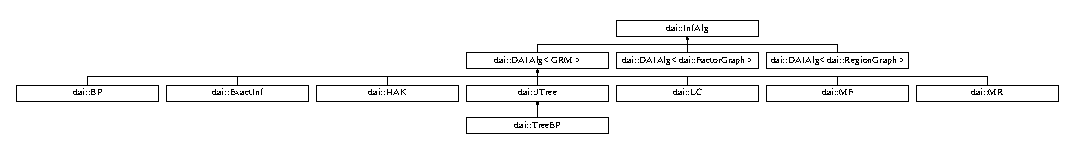
\includegraphics[height=1.56863cm]{classdai_1_1InfAlg}
\end{center}
\end{figure}


\subsection{Detailed Description}
\hyperlink{classdai_1_1InfAlg}{InfAlg} is an abstract base class, defining the common interface of all inference algorithms in libDAI. \subsection*{Public Member Functions}
\begin{CompactItemize}
\item 
\hypertarget{classdai_1_1InfAlg_00c1dba1041af038de0689cceb0a69f0}{
virtual \hyperlink{classdai_1_1InfAlg_00c1dba1041af038de0689cceb0a69f0}{$\sim$InfAlg} ()}
\label{classdai_1_1InfAlg_00c1dba1041af038de0689cceb0a69f0}

\begin{CompactList}\small\item\em Virtual desctructor (needed because this class contains virtual functions). \item\end{CompactList}\item 
\hypertarget{classdai_1_1InfAlg_28fd90657745e2a150f94d22319c6e2d}{
virtual \hyperlink{classdai_1_1InfAlg}{InfAlg} $\ast$ \hyperlink{classdai_1_1InfAlg_28fd90657745e2a150f94d22319c6e2d}{clone} () const =0}
\label{classdai_1_1InfAlg_28fd90657745e2a150f94d22319c6e2d}

\begin{CompactList}\small\item\em Returns a pointer to a new, cloned copy of $\ast$this (i.e., virtual copy constructor). \item\end{CompactList}\item 
\hypertarget{classdai_1_1InfAlg_48936a6f22a324cbe22d553ea41de7e2}{
virtual \hyperlink{classdai_1_1InfAlg}{InfAlg} $\ast$ \hyperlink{classdai_1_1InfAlg_48936a6f22a324cbe22d553ea41de7e2}{create} () const =0}
\label{classdai_1_1InfAlg_48936a6f22a324cbe22d553ea41de7e2}

\begin{CompactList}\small\item\em Returns a pointer to a newly constructed object $\ast$this (i.e., virtual default constructor). \item\end{CompactList}\item 
\hypertarget{classdai_1_1InfAlg_2f84c282ef54ab76e70fba6f823f2b27}{
virtual std::string \hyperlink{classdai_1_1InfAlg_2f84c282ef54ab76e70fba6f823f2b27}{identify} () const =0}
\label{classdai_1_1InfAlg_2f84c282ef54ab76e70fba6f823f2b27}

\begin{CompactList}\small\item\em Identifies itself for logging purposes. \item\end{CompactList}\item 
\hypertarget{classdai_1_1InfAlg_d8d8f71ea44c71905e9ee9531e3de48f}{
virtual \hyperlink{classdai_1_1TFactor}{Factor} \hyperlink{classdai_1_1InfAlg_d8d8f71ea44c71905e9ee9531e3de48f}{belief} (const \hyperlink{classdai_1_1Var}{Var} \&n) const =0}
\label{classdai_1_1InfAlg_d8d8f71ea44c71905e9ee9531e3de48f}

\begin{CompactList}\small\item\em Returns the \char`\"{}belief\char`\"{} (i.e., approximate marginal probability distribution) of a variable. \item\end{CompactList}\item 
\hypertarget{classdai_1_1InfAlg_74028032f667c44b0437019c4c13360b}{
virtual \hyperlink{classdai_1_1TFactor}{Factor} \hyperlink{classdai_1_1InfAlg_74028032f667c44b0437019c4c13360b}{belief} (const \hyperlink{classdai_1_1VarSet}{VarSet} \&n) const =0}
\label{classdai_1_1InfAlg_74028032f667c44b0437019c4c13360b}

\begin{CompactList}\small\item\em Returns the \char`\"{}belief\char`\"{} (i.e., approximate marginal probability distribution) of a set of variables. \item\end{CompactList}\item 
\hypertarget{classdai_1_1InfAlg_eac9f6b52ff7a11a1e5ac2c03bbd6eb0}{
virtual std::vector$<$ \hyperlink{classdai_1_1TFactor}{Factor} $>$ \hyperlink{classdai_1_1InfAlg_eac9f6b52ff7a11a1e5ac2c03bbd6eb0}{beliefs} () const =0}
\label{classdai_1_1InfAlg_eac9f6b52ff7a11a1e5ac2c03bbd6eb0}

\begin{CompactList}\small\item\em Returns all \char`\"{}beliefs\char`\"{} (i.e., approximate marginal probability distribution) calculated by the algorithm. \item\end{CompactList}\item 
\hypertarget{classdai_1_1InfAlg_40a2353d63c358ebca834d40b0a4fc70}{
virtual \hyperlink{namespacedai_e7d0472fdc89a8635825d01940e91cbf}{Real} \hyperlink{classdai_1_1InfAlg_40a2353d63c358ebca834d40b0a4fc70}{logZ} () const =0}
\label{classdai_1_1InfAlg_40a2353d63c358ebca834d40b0a4fc70}

\begin{CompactList}\small\item\em Returns the logarithm of the (approximated) partition sum (normalizing constant of the factor graph). \item\end{CompactList}\item 
virtual void \hyperlink{classdai_1_1InfAlg_99dd53d1aaccf09a4b977a49a983cc85}{init} ()=0
\begin{CompactList}\small\item\em Initializes all data structures of the approximate inference algorithm. \item\end{CompactList}\item 
virtual void \hyperlink{classdai_1_1InfAlg_7d006e89e01a2f3e2a40b0f7f6e37ae5}{init} (const \hyperlink{classdai_1_1VarSet}{VarSet} \&ns)=0
\begin{CompactList}\small\item\em Initializes all data structures corresponding to some set of variables. \item\end{CompactList}\item 
\hypertarget{classdai_1_1InfAlg_6b169737c142ff0be5db3dab4f4eb568}{
virtual double \hyperlink{classdai_1_1InfAlg_6b169737c142ff0be5db3dab4f4eb568}{run} ()=0}
\label{classdai_1_1InfAlg_6b169737c142ff0be5db3dab4f4eb568}

\begin{CompactList}\small\item\em Runs the approximate inference algorithm. \item\end{CompactList}\item 
\hypertarget{classdai_1_1InfAlg_25c0e975c8e615d17f72e1a6d27acfbf}{
virtual void \hyperlink{classdai_1_1InfAlg_25c0e975c8e615d17f72e1a6d27acfbf}{clamp} (const \hyperlink{classdai_1_1Var}{Var} \&n, size\_\-t i, bool backup=false)=0}
\label{classdai_1_1InfAlg_25c0e975c8e615d17f72e1a6d27acfbf}

\begin{CompactList}\small\item\em Clamp variable n to value i (i.e. multiply with a Kronecker delta $\delta_{x_n, i}$). \item\end{CompactList}\item 
\hypertarget{classdai_1_1InfAlg_2e101c9089df2d5c5761083dd5d8380f}{
virtual void \hyperlink{classdai_1_1InfAlg_2e101c9089df2d5c5761083dd5d8380f}{makeCavity} (size\_\-t i, bool backup=false)=0}
\label{classdai_1_1InfAlg_2e101c9089df2d5c5761083dd5d8380f}

\begin{CompactList}\small\item\em Set all factors interacting with var(i) to 1. \item\end{CompactList}\item 
virtual double \hyperlink{classdai_1_1InfAlg_7e1ca7da15403d5d2af4a855186c0b46}{maxDiff} () const =0
\item 
virtual size\_\-t \hyperlink{classdai_1_1InfAlg_7a93807863cc0a2025c1a78bdf1e14b8}{Iterations} () const =0
\item 
\hypertarget{classdai_1_1InfAlg_0d588a833bcd1131cf350ae85c7602c9}{
virtual \hyperlink{classdai_1_1FactorGraph}{FactorGraph} \& \hyperlink{classdai_1_1InfAlg_0d588a833bcd1131cf350ae85c7602c9}{fg} ()=0}
\label{classdai_1_1InfAlg_0d588a833bcd1131cf350ae85c7602c9}

\begin{CompactList}\small\item\em Get reference to underlying \hyperlink{classdai_1_1FactorGraph}{FactorGraph}. \item\end{CompactList}\item 
\hypertarget{classdai_1_1InfAlg_4bb40d1d0f6d7472e9211db4bea91ada}{
virtual const \hyperlink{classdai_1_1FactorGraph}{FactorGraph} \& \hyperlink{classdai_1_1InfAlg_4bb40d1d0f6d7472e9211db4bea91ada}{fg} () const =0}
\label{classdai_1_1InfAlg_4bb40d1d0f6d7472e9211db4bea91ada}

\begin{CompactList}\small\item\em Get const reference to underlying \hyperlink{classdai_1_1FactorGraph}{FactorGraph}. \item\end{CompactList}\item 
\hypertarget{classdai_1_1InfAlg_2cbc785afe9df0c6ee744d1a286b5cff}{
virtual void \hyperlink{classdai_1_1InfAlg_2cbc785afe9df0c6ee744d1a286b5cff}{backupFactor} (size\_\-t I)=0}
\label{classdai_1_1InfAlg_2cbc785afe9df0c6ee744d1a286b5cff}

\begin{CompactList}\small\item\em Save factor I. \item\end{CompactList}\item 
\hypertarget{classdai_1_1InfAlg_f3aab626dadb627e8043c2ee6461b959}{
virtual void \hyperlink{classdai_1_1InfAlg_f3aab626dadb627e8043c2ee6461b959}{backupFactors} (const \hyperlink{classdai_1_1VarSet}{VarSet} \&ns)=0}
\label{classdai_1_1InfAlg_f3aab626dadb627e8043c2ee6461b959}

\begin{CompactList}\small\item\em Save Factors involving ns. \item\end{CompactList}\item 
\hypertarget{classdai_1_1InfAlg_e8224cce01e7974b87c8b88b1aa13b59}{
virtual void \hyperlink{classdai_1_1InfAlg_e8224cce01e7974b87c8b88b1aa13b59}{restoreFactor} (size\_\-t I)=0}
\label{classdai_1_1InfAlg_e8224cce01e7974b87c8b88b1aa13b59}

\begin{CompactList}\small\item\em Restore factor I. \item\end{CompactList}\item 
\hypertarget{classdai_1_1InfAlg_fb75925b52bffea28bd25ec18fb9c070}{
virtual void \hyperlink{classdai_1_1InfAlg_fb75925b52bffea28bd25ec18fb9c070}{restoreFactors} (const \hyperlink{classdai_1_1VarSet}{VarSet} \&ns)=0}
\label{classdai_1_1InfAlg_fb75925b52bffea28bd25ec18fb9c070}

\begin{CompactList}\small\item\em Restore Factors involving ns. \item\end{CompactList}\end{CompactItemize}


\subsection{Member Function Documentation}
\hypertarget{classdai_1_1InfAlg_99dd53d1aaccf09a4b977a49a983cc85}{
\index{dai::InfAlg@{dai::InfAlg}!init@{init}}
\index{init@{init}!dai::InfAlg@{dai::InfAlg}}
\subsubsection[init]{\setlength{\rightskip}{0pt plus 5cm}virtual void dai::InfAlg::init ()\hspace{0.3cm}{\tt  \mbox{[}pure virtual\mbox{]}}}}
\label{classdai_1_1InfAlg_99dd53d1aaccf09a4b977a49a983cc85}


Initializes all data structures of the approximate inference algorithm. 

This method should be called at least once before \hyperlink{classdai_1_1InfAlg_6b169737c142ff0be5db3dab4f4eb568}{run()} is called 

Implemented in \hyperlink{classdai_1_1BP_83349319b22a2d71b1f4ef39709365f9}{dai::BP}, \hyperlink{classdai_1_1ExactInf_8b86be92502af6ef5ecb38f12406733d}{dai::ExactInf}, \hyperlink{classdai_1_1HAK_b30055f32f2c9a84d76668ff74606697}{dai::HAK}, \hyperlink{classdai_1_1JTree_cbb2df1dc4e64097a46fc4cb1394e76f}{dai::JTree}, \hyperlink{classdai_1_1LC_007ab11f0d08d0ed23ae141230b122cc}{dai::LC}, \hyperlink{classdai_1_1MF_eb993d502d0cb97424ebff82e0cf6839}{dai::MF}, \hyperlink{classdai_1_1MR_859f5c780ec490232dc7a2b8f11da38b}{dai::MR}, and \hyperlink{classdai_1_1TreeEP_fff5580fa87ce391223a2e2867527248}{dai::TreeEP}.\hypertarget{classdai_1_1InfAlg_7d006e89e01a2f3e2a40b0f7f6e37ae5}{
\index{dai::InfAlg@{dai::InfAlg}!init@{init}}
\index{init@{init}!dai::InfAlg@{dai::InfAlg}}
\subsubsection[init]{\setlength{\rightskip}{0pt plus 5cm}virtual void dai::InfAlg::init (const {\bf VarSet} \& {\em ns})\hspace{0.3cm}{\tt  \mbox{[}pure virtual\mbox{]}}}}
\label{classdai_1_1InfAlg_7d006e89e01a2f3e2a40b0f7f6e37ae5}


Initializes all data structures corresponding to some set of variables. 

This method can be used to do a partial initialization after a part of the factor graph has changed. Instead of initializing all data structures, it only initializes those involving the variables in ns. 

Implemented in \hyperlink{classdai_1_1BP_b711dcd5db848b6d993fac482b64ee20}{dai::BP}, \hyperlink{classdai_1_1ExactInf_ace58f99e40bb4084c73d6b77fd26456}{dai::ExactInf}, \hyperlink{classdai_1_1HAK_53cd01bc1e70859d556ac71b5e25a192}{dai::HAK}, \hyperlink{classdai_1_1JTree_365c52b5f264c844ac5c010026719350}{dai::JTree}, \hyperlink{classdai_1_1LC_b077c808ad6ca6b9e134746d0846ea5d}{dai::LC}, \hyperlink{classdai_1_1MF_49ddd5c9c9f51ee9fb5e153b7194ac71}{dai::MF}, \hyperlink{classdai_1_1MR_da0e0829e87b541633dbb6078529c21d}{dai::MR}, and \hyperlink{classdai_1_1TreeEP_3cc3718d1fbdf67db23a846283f99d08}{dai::TreeEP}.\hypertarget{classdai_1_1InfAlg_7e1ca7da15403d5d2af4a855186c0b46}{
\index{dai::InfAlg@{dai::InfAlg}!maxDiff@{maxDiff}}
\index{maxDiff@{maxDiff}!dai::InfAlg@{dai::InfAlg}}
\subsubsection[maxDiff]{\setlength{\rightskip}{0pt plus 5cm}virtual double dai::InfAlg::maxDiff () const\hspace{0.3cm}{\tt  \mbox{[}pure virtual\mbox{]}}}}
\label{classdai_1_1InfAlg_7e1ca7da15403d5d2af4a855186c0b46}


Return maximum difference between single node beliefs in the last pass \begin{Desc}
\item[Exceptions:]
\begin{description}
\item[{\em \hyperlink{classdai_1_1Exception}{Exception}}]if not implemented/supported \end{description}
\end{Desc}


Implemented in \hyperlink{classdai_1_1BP_9954b795f95ae1730d4e09a06afd8ee4}{dai::BP}, \hyperlink{classdai_1_1ExactInf_4f3189ff1567e80dd245a1308f1f31bf}{dai::ExactInf}, \hyperlink{classdai_1_1HAK_1eb4c5a84c30f7c8db8b8f4c0c54f567}{dai::HAK}, \hyperlink{classdai_1_1JTree_acd3916835c9d349aa1b22a2dd54de83}{dai::JTree}, \hyperlink{classdai_1_1LC_32b30963958c3f408d1c5a618fcf418d}{dai::LC}, \hyperlink{classdai_1_1MF_032b149026f011a5cbcd01eb08a3b8dc}{dai::MF}, \hyperlink{classdai_1_1MR_a55d0a62912e9fe8a685157cfa309918}{dai::MR}, and \hyperlink{classdai_1_1TreeEP_d1214cd7bc0899d1a8dc4523bacdb488}{dai::TreeEP}.\hypertarget{classdai_1_1InfAlg_7a93807863cc0a2025c1a78bdf1e14b8}{
\index{dai::InfAlg@{dai::InfAlg}!Iterations@{Iterations}}
\index{Iterations@{Iterations}!dai::InfAlg@{dai::InfAlg}}
\subsubsection[Iterations]{\setlength{\rightskip}{0pt plus 5cm}virtual size\_\-t dai::InfAlg::Iterations () const\hspace{0.3cm}{\tt  \mbox{[}pure virtual\mbox{]}}}}
\label{classdai_1_1InfAlg_7a93807863cc0a2025c1a78bdf1e14b8}


Return number of passes over the factorgraph \begin{Desc}
\item[Exceptions:]
\begin{description}
\item[{\em \hyperlink{classdai_1_1Exception}{Exception}}]if not implemented/supported \end{description}
\end{Desc}


Implemented in \hyperlink{classdai_1_1BP_be6cbc2992d38144198c8f4ea731a26e}{dai::BP}, \hyperlink{classdai_1_1ExactInf_2df22866419ee923043c8fcf0a2ff62b}{dai::ExactInf}, \hyperlink{classdai_1_1HAK_27599fc844670e503786ac5d485713c5}{dai::HAK}, \hyperlink{classdai_1_1JTree_71cd98f072d69f6ce60af8b52ef02eb8}{dai::JTree}, \hyperlink{classdai_1_1LC_8654c28fad78fa6cd850b2207b271086}{dai::LC}, \hyperlink{classdai_1_1MF_e2daf3cd007572d19d6156f2484db4fd}{dai::MF}, \hyperlink{classdai_1_1MR_6a199aa1d43b3c143a4b631735f53ee3}{dai::MR}, and \hyperlink{classdai_1_1TreeEP_e18e681d1f078e42445d39f8605df7d4}{dai::TreeEP}.

The documentation for this class was generated from the following file:\begin{CompactItemize}
\item 
include/dai/\hyperlink{daialg_8h}{daialg.h}\end{CompactItemize}

\hypertarget{classdai_1_1JTree}{
\section{dai::JTree Class Reference}
\label{classdai_1_1JTree}\index{dai::JTree@{dai::JTree}}
}
{\tt \#include $<$dai/jtree.h$>$}

Inheritance diagram for dai::JTree::\begin{figure}[H]
\begin{center}
\leavevmode
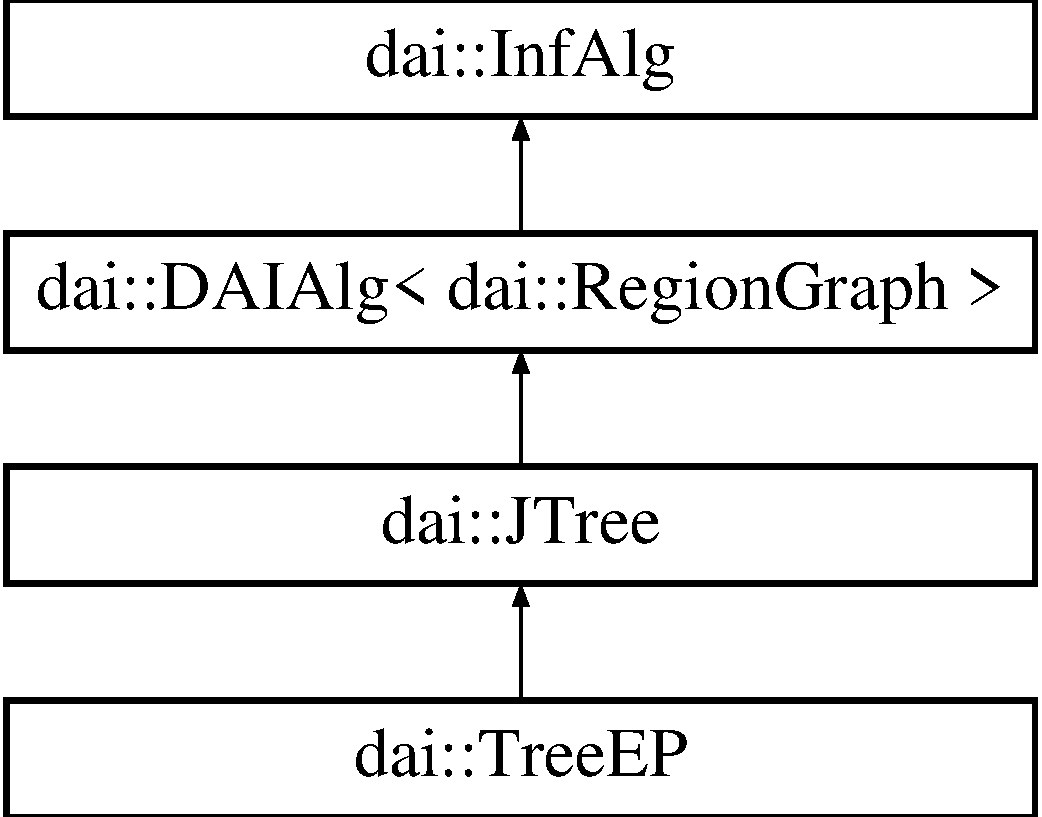
\includegraphics[height=4cm]{classdai_1_1JTree}
\end{center}
\end{figure}


\subsection{Detailed Description}
Exact inference algorithm using junction tree. \subsection*{Public Member Functions}
\begin{CompactItemize}
\item 
\hypertarget{classdai_1_1JTree_7e4dd4e6f6eaded0600b6759ceccae87}{
\hyperlink{classdai_1_1JTree_7e4dd4e6f6eaded0600b6759ceccae87}{JTree} ()}
\label{classdai_1_1JTree_7e4dd4e6f6eaded0600b6759ceccae87}

\begin{CompactList}\small\item\em Default constructor. \item\end{CompactList}\item 
\hypertarget{classdai_1_1JTree_48999aa576e174177e5f904deaa9699d}{
\hyperlink{classdai_1_1JTree_48999aa576e174177e5f904deaa9699d}{JTree} (const \hyperlink{classdai_1_1JTree}{JTree} \&x)}
\label{classdai_1_1JTree_48999aa576e174177e5f904deaa9699d}

\begin{CompactList}\small\item\em Copy constructor. \item\end{CompactList}\item 
\hypertarget{classdai_1_1JTree_e57eeabbe31424e37ede02ec83d8c89b}{
\hyperlink{classdai_1_1JTree}{JTree} \& \hyperlink{classdai_1_1JTree_e57eeabbe31424e37ede02ec83d8c89b}{operator=} (const \hyperlink{classdai_1_1JTree}{JTree} \&x)}
\label{classdai_1_1JTree_e57eeabbe31424e37ede02ec83d8c89b}

\begin{CompactList}\small\item\em Assignment operator. \item\end{CompactList}\item 
\hypertarget{classdai_1_1JTree_5c81f2500cc196eb50921d7db7794216}{
\hyperlink{classdai_1_1JTree_5c81f2500cc196eb50921d7db7794216}{JTree} (const \hyperlink{classdai_1_1FactorGraph}{FactorGraph} \&fg, const \hyperlink{classdai_1_1PropertySet}{PropertySet} \&opts, bool automatic=true)}
\label{classdai_1_1JTree_5c81f2500cc196eb50921d7db7794216}

\begin{CompactList}\small\item\em Construct from \hyperlink{classdai_1_1FactorGraph}{FactorGraph} fg and \hyperlink{classdai_1_1PropertySet}{PropertySet} opts. \item\end{CompactList}\item 
\hypertarget{classdai_1_1DAIAlg_48ba6a58d10b8802d690e5e92ec5abe9}{
void \hyperlink{classdai_1_1DAIAlg_48ba6a58d10b8802d690e5e92ec5abe9}{backupFactor} (size\_\-t I)}
\label{classdai_1_1DAIAlg_48ba6a58d10b8802d690e5e92ec5abe9}

\begin{CompactList}\small\item\em Save factor I. \item\end{CompactList}\item 
\hypertarget{classdai_1_1DAIAlg_0176904d3b4b9d083288ea8c4a2dc8bc}{
void \hyperlink{classdai_1_1DAIAlg_0176904d3b4b9d083288ea8c4a2dc8bc}{backupFactors} (const \hyperlink{classdai_1_1VarSet}{VarSet} \&ns)}
\label{classdai_1_1DAIAlg_0176904d3b4b9d083288ea8c4a2dc8bc}

\begin{CompactList}\small\item\em Save Factors involving ns. \item\end{CompactList}\item 
\hypertarget{classdai_1_1DAIAlg_bf8dbd2797ec871e86566a6dfc0864e3}{
void \hyperlink{classdai_1_1DAIAlg_bf8dbd2797ec871e86566a6dfc0864e3}{restoreFactor} (size\_\-t I)}
\label{classdai_1_1DAIAlg_bf8dbd2797ec871e86566a6dfc0864e3}

\begin{CompactList}\small\item\em Restore factor I. \item\end{CompactList}\item 
\hypertarget{classdai_1_1DAIAlg_3ce97e9370f1cdc785526c1a6c1eaadf}{
void \hyperlink{classdai_1_1DAIAlg_3ce97e9370f1cdc785526c1a6c1eaadf}{restoreFactors} (const \hyperlink{classdai_1_1VarSet}{VarSet} \&ns)}
\label{classdai_1_1DAIAlg_3ce97e9370f1cdc785526c1a6c1eaadf}

\begin{CompactList}\small\item\em Restore Factors involving ns. \item\end{CompactList}\item 
\hypertarget{classdai_1_1DAIAlg_b7d537f1a9d116617d8dce722ce65dc0}{
void \hyperlink{classdai_1_1DAIAlg_b7d537f1a9d116617d8dce722ce65dc0}{clamp} (const \hyperlink{classdai_1_1Var}{Var} \&n, size\_\-t i, bool backup=false)}
\label{classdai_1_1DAIAlg_b7d537f1a9d116617d8dce722ce65dc0}

\begin{CompactList}\small\item\em Clamp variable n to value i (i.e. multiply with a Kronecker delta $\delta_{x_n, i}$). \item\end{CompactList}\item 
\hypertarget{classdai_1_1DAIAlg_7f0b8452352080a1e35ab9a68cb589fd}{
void \hyperlink{classdai_1_1DAIAlg_7f0b8452352080a1e35ab9a68cb589fd}{makeCavity} (size\_\-t i, bool backup=false)}
\label{classdai_1_1DAIAlg_7f0b8452352080a1e35ab9a68cb589fd}

\begin{CompactList}\small\item\em Set all factors interacting with var(i) to 1. \item\end{CompactList}\item 
\hypertarget{classdai_1_1DAIAlg_9348542c22d04ed804388f1fe3009fa3}{
\hyperlink{classdai_1_1FactorGraph}{FactorGraph} \& \hyperlink{classdai_1_1DAIAlg_9348542c22d04ed804388f1fe3009fa3}{fg} ()}
\label{classdai_1_1DAIAlg_9348542c22d04ed804388f1fe3009fa3}

\begin{CompactList}\small\item\em Get reference to underlying \hyperlink{classdai_1_1FactorGraph}{FactorGraph}. \item\end{CompactList}\item 
\hypertarget{classdai_1_1DAIAlg_35400e471b8c3c98bef6c74ceac8fa16}{
const \hyperlink{classdai_1_1FactorGraph}{FactorGraph} \& \hyperlink{classdai_1_1DAIAlg_35400e471b8c3c98bef6c74ceac8fa16}{fg} () const }
\label{classdai_1_1DAIAlg_35400e471b8c3c98bef6c74ceac8fa16}

\begin{CompactList}\small\item\em Get const reference to underlying \hyperlink{classdai_1_1FactorGraph}{FactorGraph}. \item\end{CompactList}\end{CompactItemize}
\begin{Indent}{\bf General InfAlg interface}\par
\begin{CompactItemize}
\item 
\hypertarget{classdai_1_1JTree_54c62d9fb8ac3f12b06343989c6fd398}{
virtual \hyperlink{classdai_1_1JTree}{JTree} $\ast$ \hyperlink{classdai_1_1JTree_54c62d9fb8ac3f12b06343989c6fd398}{clone} () const }
\label{classdai_1_1JTree_54c62d9fb8ac3f12b06343989c6fd398}

\begin{CompactList}\small\item\em Returns a pointer to a new, cloned copy of $\ast$this (i.e., virtual copy constructor). \item\end{CompactList}\item 
\hypertarget{classdai_1_1JTree_0a4a6ba17b04d274fec3dbebc6a2a6cb}{
virtual \hyperlink{classdai_1_1JTree}{JTree} $\ast$ \hyperlink{classdai_1_1JTree_0a4a6ba17b04d274fec3dbebc6a2a6cb}{create} () const }
\label{classdai_1_1JTree_0a4a6ba17b04d274fec3dbebc6a2a6cb}

\begin{CompactList}\small\item\em Returns a pointer to a newly constructed object $\ast$this (i.e., virtual default constructor). \item\end{CompactList}\item 
\hypertarget{classdai_1_1JTree_bc4d34db1bd656b35e430a1e26388aa1}{
virtual std::string \hyperlink{classdai_1_1JTree_bc4d34db1bd656b35e430a1e26388aa1}{identify} () const }
\label{classdai_1_1JTree_bc4d34db1bd656b35e430a1e26388aa1}

\begin{CompactList}\small\item\em Identifies itself for logging purposes. \item\end{CompactList}\item 
\hypertarget{classdai_1_1JTree_432cdc9cc9f4be26509e6bd2337c5325}{
virtual \hyperlink{classdai_1_1TFactor}{Factor} \hyperlink{classdai_1_1JTree_432cdc9cc9f4be26509e6bd2337c5325}{belief} (const \hyperlink{classdai_1_1Var}{Var} \&n) const }
\label{classdai_1_1JTree_432cdc9cc9f4be26509e6bd2337c5325}

\begin{CompactList}\small\item\em Returns the \char`\"{}belief\char`\"{} (i.e., approximate marginal probability distribution) of a variable. \item\end{CompactList}\item 
\hypertarget{classdai_1_1JTree_10de7513fea42d8c02be95a30bb69553}{
virtual \hyperlink{classdai_1_1TFactor}{Factor} \hyperlink{classdai_1_1JTree_10de7513fea42d8c02be95a30bb69553}{belief} (const \hyperlink{classdai_1_1VarSet}{VarSet} \&ns) const }
\label{classdai_1_1JTree_10de7513fea42d8c02be95a30bb69553}

\begin{CompactList}\small\item\em Returns the \char`\"{}belief\char`\"{} (i.e., approximate marginal probability distribution) of a set of variables. \item\end{CompactList}\item 
\hypertarget{classdai_1_1JTree_3c16a15fe017649fec4d63455fda6843}{
virtual std::vector$<$ \hyperlink{classdai_1_1TFactor}{Factor} $>$ \hyperlink{classdai_1_1JTree_3c16a15fe017649fec4d63455fda6843}{beliefs} () const }
\label{classdai_1_1JTree_3c16a15fe017649fec4d63455fda6843}

\begin{CompactList}\small\item\em Returns all \char`\"{}beliefs\char`\"{} (i.e., approximate marginal probability distribution) calculated by the algorithm. \item\end{CompactList}\item 
\hypertarget{classdai_1_1JTree_d2e2c9ff0327014da4c41d211bfd57c5}{
virtual \hyperlink{namespacedai_e7d0472fdc89a8635825d01940e91cbf}{Real} \hyperlink{classdai_1_1JTree_d2e2c9ff0327014da4c41d211bfd57c5}{logZ} () const }
\label{classdai_1_1JTree_d2e2c9ff0327014da4c41d211bfd57c5}

\begin{CompactList}\small\item\em Returns the logarithm of the (approximated) partition sum (normalizing constant of the factor graph). \item\end{CompactList}\item 
virtual void \hyperlink{classdai_1_1JTree_cbb2df1dc4e64097a46fc4cb1394e76f}{init} ()
\begin{CompactList}\small\item\em Initializes all data structures of the approximate inference algorithm. \item\end{CompactList}\item 
virtual void \hyperlink{classdai_1_1JTree_365c52b5f264c844ac5c010026719350}{init} (const \hyperlink{classdai_1_1VarSet}{VarSet} \&)
\begin{CompactList}\small\item\em Initializes all data structures corresponding to some set of variables. \item\end{CompactList}\item 
\hypertarget{classdai_1_1JTree_b0cd2ba167212e4c8c8d241b985d3db6}{
virtual double \hyperlink{classdai_1_1JTree_b0cd2ba167212e4c8c8d241b985d3db6}{run} ()}
\label{classdai_1_1JTree_b0cd2ba167212e4c8c8d241b985d3db6}

\begin{CompactList}\small\item\em Runs the approximate inference algorithm. \item\end{CompactList}\item 
virtual double \hyperlink{classdai_1_1JTree_acd3916835c9d349aa1b22a2dd54de83}{maxDiff} () const 
\item 
virtual size\_\-t \hyperlink{classdai_1_1JTree_71cd98f072d69f6ce60af8b52ef02eb8}{Iterations} () const 
\end{CompactItemize}
\end{Indent}
\begin{Indent}{\bf Additional interface specific for JTree}\par
\begin{CompactItemize}
\item 
\hypertarget{classdai_1_1JTree_0898a401baee9af694f636d174048a46}{
void \textbf{GenerateJT} (const std::vector$<$ \hyperlink{classdai_1_1VarSet}{VarSet} $>$ \&Cliques)}
\label{classdai_1_1JTree_0898a401baee9af694f636d174048a46}

\item 
\hypertarget{classdai_1_1JTree_5a96942bd16a4e4e10fcf720c1b0e04b}{
\hyperlink{classdai_1_1TFactor}{Factor} \& \hyperlink{classdai_1_1JTree_5a96942bd16a4e4e10fcf720c1b0e04b}{message} (size\_\-t alpha, size\_\-t \_\-beta)}
\label{classdai_1_1JTree_5a96942bd16a4e4e10fcf720c1b0e04b}

\begin{CompactList}\small\item\em Returns reference the message from outer region alpha to its \_\-beta'th neighboring inner region. \item\end{CompactList}\item 
\hypertarget{classdai_1_1JTree_e59c0012cbd6a425704fd637f9fed4c5}{
const \hyperlink{classdai_1_1TFactor}{Factor} \& \hyperlink{classdai_1_1JTree_e59c0012cbd6a425704fd637f9fed4c5}{message} (size\_\-t alpha, size\_\-t \_\-beta) const }
\label{classdai_1_1JTree_e59c0012cbd6a425704fd637f9fed4c5}

\begin{CompactList}\small\item\em Returns const reference to the message from outer region alpha to its \_\-beta'th neighboring inner region. \item\end{CompactList}\item 
\hypertarget{classdai_1_1JTree_4569d21624cb49d9a79c3c8332e0d4b3}{
void \hyperlink{classdai_1_1JTree_4569d21624cb49d9a79c3c8332e0d4b3}{runHUGIN} ()}
\label{classdai_1_1JTree_4569d21624cb49d9a79c3c8332e0d4b3}

\begin{CompactList}\small\item\em Runs junction-tree with HUGIN updates. \item\end{CompactList}\item 
\hypertarget{classdai_1_1JTree_6d8ee4f30498985d0d434988dba8c258}{
void \hyperlink{classdai_1_1JTree_6d8ee4f30498985d0d434988dba8c258}{runShaferShenoy} ()}
\label{classdai_1_1JTree_6d8ee4f30498985d0d434988dba8c258}

\begin{CompactList}\small\item\em Runs junction-tree with Shafer-Shenoy updates. \item\end{CompactList}\item 
\hypertarget{classdai_1_1JTree_0ee81ed10535369928ba0abb3c1f7e02}{
size\_\-t \hyperlink{classdai_1_1JTree_0ee81ed10535369928ba0abb3c1f7e02}{findEfficientTree} (const \hyperlink{classdai_1_1VarSet}{VarSet} \&ns, \hyperlink{namespacedai_e7764251ab4d4b2d4fbec214eac83079}{DEdgeVec} \&Tree, size\_\-t PreviousRoot=(size\_\-t)-1) const }
\label{classdai_1_1JTree_0ee81ed10535369928ba0abb3c1f7e02}

\begin{CompactList}\small\item\em Finds an efficient tree for calculating the marginal of some variables. \item\end{CompactList}\item 
\hypertarget{classdai_1_1JTree_2ffd2a47a85b81efbbb5f0cfd7a083fa}{
\hyperlink{classdai_1_1TFactor}{Factor} \hyperlink{classdai_1_1JTree_2ffd2a47a85b81efbbb5f0cfd7a083fa}{calcMarginal} (const \hyperlink{classdai_1_1VarSet}{VarSet} \&ns)}
\label{classdai_1_1JTree_2ffd2a47a85b81efbbb5f0cfd7a083fa}

\begin{CompactList}\small\item\em Calculates the marginal of a set of variables. \item\end{CompactList}\end{CompactItemize}
\end{Indent}
\subsection*{Public Attributes}
\begin{CompactItemize}
\item 
\hypertarget{classdai_1_1JTree_6ddedae95e2dda19e20b7b49455ea389}{
\hyperlink{namespacedai_e7764251ab4d4b2d4fbec214eac83079}{DEdgeVec} \hyperlink{classdai_1_1JTree_6ddedae95e2dda19e20b7b49455ea389}{RTree}}
\label{classdai_1_1JTree_6ddedae95e2dda19e20b7b49455ea389}

\begin{CompactList}\small\item\em Rooted tree. \item\end{CompactList}\item 
\hypertarget{classdai_1_1JTree_66cdd4d8258582aaf794466f3786dbfb}{
std::vector$<$ \hyperlink{classdai_1_1TFactor}{Factor} $>$ \hyperlink{classdai_1_1JTree_66cdd4d8258582aaf794466f3786dbfb}{Qa}}
\label{classdai_1_1JTree_66cdd4d8258582aaf794466f3786dbfb}

\begin{CompactList}\small\item\em Outer region beliefs. \item\end{CompactList}\item 
\hypertarget{classdai_1_1JTree_9d93e9f387d9772be5bc2b5372f7d20d}{
std::vector$<$ \hyperlink{classdai_1_1TFactor}{Factor} $>$ \hyperlink{classdai_1_1JTree_9d93e9f387d9772be5bc2b5372f7d20d}{Qb}}
\label{classdai_1_1JTree_9d93e9f387d9772be5bc2b5372f7d20d}

\begin{CompactList}\small\item\em Inner region beliefs. \item\end{CompactList}\item 
\hypertarget{classdai_1_1JTree_9bcd565eb07149a7aeeb0380e042036c}{
struct \hyperlink{structdai_1_1JTree_1_1Properties}{dai::JTree::Properties} \hyperlink{classdai_1_1JTree_9bcd565eb07149a7aeeb0380e042036c}{props}}
\label{classdai_1_1JTree_9bcd565eb07149a7aeeb0380e042036c}

\begin{CompactList}\small\item\em Parameters of this inference algorithm. \item\end{CompactList}\end{CompactItemize}
\subsection*{Static Public Attributes}
\begin{CompactItemize}
\item 
\hypertarget{classdai_1_1JTree_e7c0a2ebb2675cb6f8441eae09f7f826}{
static const char $\ast$ \hyperlink{classdai_1_1JTree_e7c0a2ebb2675cb6f8441eae09f7f826}{Name} = \char`\"{}JTREE\char`\"{}}
\label{classdai_1_1JTree_e7c0a2ebb2675cb6f8441eae09f7f826}

\begin{CompactList}\small\item\em Name of this inference algorithm. \item\end{CompactList}\end{CompactItemize}
\subsection*{Related Functions}
(Note that these are not member functions.) \begin{CompactItemize}
\item 
std::pair$<$ size\_\-t, size\_\-t $>$ \hyperlink{classdai_1_1JTree_bca2633ffb8701cb62c54241bdad307e}{treewidth} (const \hyperlink{classdai_1_1FactorGraph}{FactorGraph} \&fg)
\begin{CompactList}\small\item\em Calculates upper bound to the treewidth of a \hyperlink{classdai_1_1FactorGraph}{FactorGraph}. \item\end{CompactList}\end{CompactItemize}
\subsection*{Classes}
\begin{CompactItemize}
\item 
struct \hyperlink{structdai_1_1JTree_1_1Properties}{Properties}
\begin{CompactList}\small\item\em Parameters of this inference algorithm. \item\end{CompactList}\end{CompactItemize}


\subsection{Member Function Documentation}
\hypertarget{classdai_1_1JTree_cbb2df1dc4e64097a46fc4cb1394e76f}{
\index{dai::JTree@{dai::JTree}!init@{init}}
\index{init@{init}!dai::JTree@{dai::JTree}}
\subsubsection[init]{\setlength{\rightskip}{0pt plus 5cm}virtual void dai::JTree::init ()\hspace{0.3cm}{\tt  \mbox{[}inline, virtual\mbox{]}}}}
\label{classdai_1_1JTree_cbb2df1dc4e64097a46fc4cb1394e76f}


Initializes all data structures of the approximate inference algorithm. 

This method should be called at least once before \hyperlink{classdai_1_1JTree_b0cd2ba167212e4c8c8d241b985d3db6}{run()} is called 

Implements \hyperlink{classdai_1_1InfAlg_99dd53d1aaccf09a4b977a49a983cc85}{dai::InfAlg}.

Reimplemented in \hyperlink{classdai_1_1TreeEP_fff5580fa87ce391223a2e2867527248}{dai::TreeEP}.\hypertarget{classdai_1_1JTree_365c52b5f264c844ac5c010026719350}{
\index{dai::JTree@{dai::JTree}!init@{init}}
\index{init@{init}!dai::JTree@{dai::JTree}}
\subsubsection[init]{\setlength{\rightskip}{0pt plus 5cm}virtual void dai::JTree::init (const {\bf VarSet} \& {\em ns})\hspace{0.3cm}{\tt  \mbox{[}inline, virtual\mbox{]}}}}
\label{classdai_1_1JTree_365c52b5f264c844ac5c010026719350}


Initializes all data structures corresponding to some set of variables. 

This method can be used to do a partial initialization after a part of the factor graph has changed. Instead of initializing all data structures, it only initializes those involving the variables in ns. 

Implements \hyperlink{classdai_1_1InfAlg_7d006e89e01a2f3e2a40b0f7f6e37ae5}{dai::InfAlg}.

Reimplemented in \hyperlink{classdai_1_1TreeEP_3cc3718d1fbdf67db23a846283f99d08}{dai::TreeEP}.\hypertarget{classdai_1_1JTree_acd3916835c9d349aa1b22a2dd54de83}{
\index{dai::JTree@{dai::JTree}!maxDiff@{maxDiff}}
\index{maxDiff@{maxDiff}!dai::JTree@{dai::JTree}}
\subsubsection[maxDiff]{\setlength{\rightskip}{0pt plus 5cm}virtual double dai::JTree::maxDiff () const\hspace{0.3cm}{\tt  \mbox{[}inline, virtual\mbox{]}}}}
\label{classdai_1_1JTree_acd3916835c9d349aa1b22a2dd54de83}


Return maximum difference between single node beliefs in the last pass \begin{Desc}
\item[Exceptions:]
\begin{description}
\item[{\em \hyperlink{classdai_1_1Exception}{Exception}}]if not implemented/supported \end{description}
\end{Desc}


Implements \hyperlink{classdai_1_1InfAlg_7e1ca7da15403d5d2af4a855186c0b46}{dai::InfAlg}.

Reimplemented in \hyperlink{classdai_1_1TreeEP_d1214cd7bc0899d1a8dc4523bacdb488}{dai::TreeEP}.\hypertarget{classdai_1_1JTree_71cd98f072d69f6ce60af8b52ef02eb8}{
\index{dai::JTree@{dai::JTree}!Iterations@{Iterations}}
\index{Iterations@{Iterations}!dai::JTree@{dai::JTree}}
\subsubsection[Iterations]{\setlength{\rightskip}{0pt plus 5cm}virtual size\_\-t dai::JTree::Iterations () const\hspace{0.3cm}{\tt  \mbox{[}inline, virtual\mbox{]}}}}
\label{classdai_1_1JTree_71cd98f072d69f6ce60af8b52ef02eb8}


Return number of passes over the factorgraph \begin{Desc}
\item[Exceptions:]
\begin{description}
\item[{\em \hyperlink{classdai_1_1Exception}{Exception}}]if not implemented/supported \end{description}
\end{Desc}


Implements \hyperlink{classdai_1_1InfAlg_7a93807863cc0a2025c1a78bdf1e14b8}{dai::InfAlg}.

Reimplemented in \hyperlink{classdai_1_1TreeEP_e18e681d1f078e42445d39f8605df7d4}{dai::TreeEP}.

\subsection{Friends And Related Function Documentation}
\hypertarget{classdai_1_1JTree_bca2633ffb8701cb62c54241bdad307e}{
\index{dai::JTree@{dai::JTree}!treewidth@{treewidth}}
\index{treewidth@{treewidth}!dai::JTree@{dai::JTree}}
\subsubsection[treewidth]{\setlength{\rightskip}{0pt plus 5cm}std::pair$<$ size\_\-t, size\_\-t $>$ treewidth (const {\bf FactorGraph} \& {\em fg})\hspace{0.3cm}{\tt  \mbox{[}related\mbox{]}}}}
\label{classdai_1_1JTree_bca2633ffb8701cb62c54241bdad307e}


Calculates upper bound to the treewidth of a \hyperlink{classdai_1_1FactorGraph}{FactorGraph}. 

\begin{Desc}
\item[Returns:]a pair (number of variables in largest clique, number of states in largest clique) \end{Desc}


The documentation for this class was generated from the following files:\begin{CompactItemize}
\item 
include/dai/\hyperlink{jtree_8h}{jtree.h}\item 
src/jtree.cpp\end{CompactItemize}

\hypertarget{structdai_1_1JTree_1_1Properties}{
\section{dai::JTree::Properties Struct Reference}
\label{structdai_1_1JTree_1_1Properties}\index{dai::JTree::Properties@{dai::JTree::Properties}}
}
{\tt \#include $<$dai/jtree.h$>$}



\subsection{Detailed Description}
Parameters of this inference algorithm. \subsection*{Public Attributes}
\begin{CompactItemize}
\item 
size\_\-t \hyperlink{structdai_1_1JTree_1_1Properties_f1115a3a2efbb2047f4305f3e88e364d}{verbose}
\begin{CompactList}\small\item\em Enumeration of possible \hyperlink{classdai_1_1JTree}{JTree} updates. \item\end{CompactList}\item 
\hypertarget{structdai_1_1JTree_1_1Properties_9120abdd0ab3d1456cc25526013df494}{
UpdateType \hyperlink{structdai_1_1JTree_1_1Properties_9120abdd0ab3d1456cc25526013df494}{updates}}
\label{structdai_1_1JTree_1_1Properties_9120abdd0ab3d1456cc25526013df494}

\begin{CompactList}\small\item\em Type of updates. \item\end{CompactList}\end{CompactItemize}


\subsection{Member Data Documentation}
\hypertarget{structdai_1_1JTree_1_1Properties_f1115a3a2efbb2047f4305f3e88e364d}{
\index{dai::JTree::Properties@{dai::JTree::Properties}!verbose@{verbose}}
\index{verbose@{verbose}!dai::JTree::Properties@{dai::JTree::Properties}}
\subsubsection[verbose]{\setlength{\rightskip}{0pt plus 5cm}size\_\-t {\bf dai::JTree::Properties::verbose}}}
\label{structdai_1_1JTree_1_1Properties_f1115a3a2efbb2047f4305f3e88e364d}


Enumeration of possible \hyperlink{classdai_1_1JTree}{JTree} updates. 

Verbosity 

The documentation for this struct was generated from the following file:\begin{CompactItemize}
\item 
include/dai/\hyperlink{jtree_8h}{jtree.h}\end{CompactItemize}

\hypertarget{classdai_1_1LC}{
\section{dai::LC Class Reference}
\label{classdai_1_1LC}\index{dai::LC@{dai::LC}}
}
{\tt \#include $<$dai/lc.h$>$}

Inheritance diagram for dai::LC::\begin{figure}[H]
\begin{center}
\leavevmode
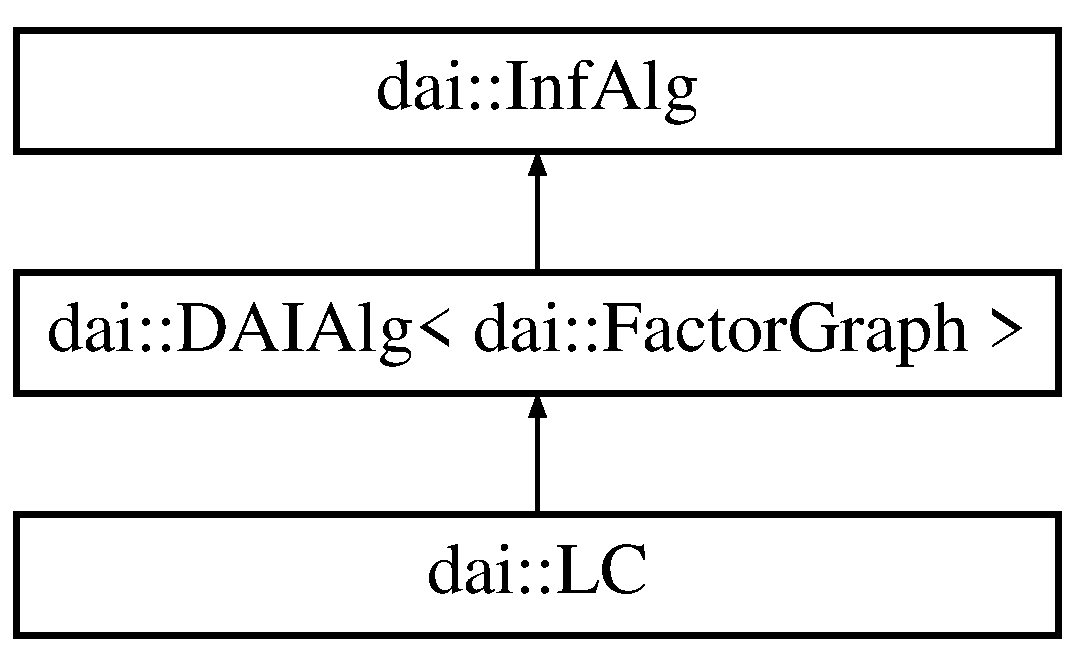
\includegraphics[height=3cm]{classdai_1_1LC}
\end{center}
\end{figure}


\subsection{Detailed Description}
Approximate inference algorithm \char`\"{}Loop Corrected Belief Propagation\char`\"{} by Mooij and Kappen. \subsection*{Public Member Functions}
\begin{CompactItemize}
\item 
\hypertarget{classdai_1_1LC_e46e76de9def71e83ff7d95604e641b4}{
\hyperlink{classdai_1_1LC_e46e76de9def71e83ff7d95604e641b4}{LC} ()}
\label{classdai_1_1LC_e46e76de9def71e83ff7d95604e641b4}

\begin{CompactList}\small\item\em Default constructor. \item\end{CompactList}\item 
\hypertarget{classdai_1_1LC_2f9f79af763757bbc8507e63c0440a27}{
\hyperlink{classdai_1_1LC_2f9f79af763757bbc8507e63c0440a27}{LC} (const \hyperlink{classdai_1_1LC}{LC} \&x)}
\label{classdai_1_1LC_2f9f79af763757bbc8507e63c0440a27}

\begin{CompactList}\small\item\em Copy constructor. \item\end{CompactList}\item 
\hypertarget{classdai_1_1LC_d8650f8491916e9d9fd96f2b9a76ed53}{
\hyperlink{classdai_1_1LC}{LC} \& \hyperlink{classdai_1_1LC_d8650f8491916e9d9fd96f2b9a76ed53}{operator=} (const \hyperlink{classdai_1_1LC}{LC} \&x)}
\label{classdai_1_1LC_d8650f8491916e9d9fd96f2b9a76ed53}

\begin{CompactList}\small\item\em Assignment operator. \item\end{CompactList}\item 
\hypertarget{classdai_1_1LC_f7876f0893b969c4d2842927085c18e3}{
\hyperlink{classdai_1_1LC_f7876f0893b969c4d2842927085c18e3}{LC} (const \hyperlink{classdai_1_1FactorGraph}{FactorGraph} \&fg, const \hyperlink{classdai_1_1PropertySet}{PropertySet} \&opts)}
\label{classdai_1_1LC_f7876f0893b969c4d2842927085c18e3}

\begin{CompactList}\small\item\em Construct from \hyperlink{classdai_1_1FactorGraph}{FactorGraph} fg and \hyperlink{classdai_1_1PropertySet}{PropertySet} opts. \item\end{CompactList}\item 
\hypertarget{classdai_1_1DAIAlg_48ba6a58d10b8802d690e5e92ec5abe9}{
void \hyperlink{classdai_1_1DAIAlg_48ba6a58d10b8802d690e5e92ec5abe9}{backupFactor} (size\_\-t I)}
\label{classdai_1_1DAIAlg_48ba6a58d10b8802d690e5e92ec5abe9}

\begin{CompactList}\small\item\em Save factor I. \item\end{CompactList}\item 
\hypertarget{classdai_1_1DAIAlg_0176904d3b4b9d083288ea8c4a2dc8bc}{
void \hyperlink{classdai_1_1DAIAlg_0176904d3b4b9d083288ea8c4a2dc8bc}{backupFactors} (const \hyperlink{classdai_1_1VarSet}{VarSet} \&ns)}
\label{classdai_1_1DAIAlg_0176904d3b4b9d083288ea8c4a2dc8bc}

\begin{CompactList}\small\item\em Save Factors involving ns. \item\end{CompactList}\item 
\hypertarget{classdai_1_1DAIAlg_bf8dbd2797ec871e86566a6dfc0864e3}{
void \hyperlink{classdai_1_1DAIAlg_bf8dbd2797ec871e86566a6dfc0864e3}{restoreFactor} (size\_\-t I)}
\label{classdai_1_1DAIAlg_bf8dbd2797ec871e86566a6dfc0864e3}

\begin{CompactList}\small\item\em Restore factor I. \item\end{CompactList}\item 
\hypertarget{classdai_1_1DAIAlg_3ce97e9370f1cdc785526c1a6c1eaadf}{
void \hyperlink{classdai_1_1DAIAlg_3ce97e9370f1cdc785526c1a6c1eaadf}{restoreFactors} (const \hyperlink{classdai_1_1VarSet}{VarSet} \&ns)}
\label{classdai_1_1DAIAlg_3ce97e9370f1cdc785526c1a6c1eaadf}

\begin{CompactList}\small\item\em Restore Factors involving ns. \item\end{CompactList}\item 
\hypertarget{classdai_1_1DAIAlg_b7d537f1a9d116617d8dce722ce65dc0}{
void \hyperlink{classdai_1_1DAIAlg_b7d537f1a9d116617d8dce722ce65dc0}{clamp} (const \hyperlink{classdai_1_1Var}{Var} \&n, size\_\-t i, bool backup=false)}
\label{classdai_1_1DAIAlg_b7d537f1a9d116617d8dce722ce65dc0}

\begin{CompactList}\small\item\em Clamp variable n to value i (i.e. multiply with a Kronecker delta $\delta_{x_n, i}$). \item\end{CompactList}\item 
\hypertarget{classdai_1_1DAIAlg_7f0b8452352080a1e35ab9a68cb589fd}{
void \hyperlink{classdai_1_1DAIAlg_7f0b8452352080a1e35ab9a68cb589fd}{makeCavity} (size\_\-t i, bool backup=false)}
\label{classdai_1_1DAIAlg_7f0b8452352080a1e35ab9a68cb589fd}

\begin{CompactList}\small\item\em Set all factors interacting with var(i) to 1. \item\end{CompactList}\item 
\hypertarget{classdai_1_1DAIAlg_9348542c22d04ed804388f1fe3009fa3}{
\hyperlink{classdai_1_1FactorGraph}{FactorGraph} \& \hyperlink{classdai_1_1DAIAlg_9348542c22d04ed804388f1fe3009fa3}{fg} ()}
\label{classdai_1_1DAIAlg_9348542c22d04ed804388f1fe3009fa3}

\begin{CompactList}\small\item\em Get reference to underlying \hyperlink{classdai_1_1FactorGraph}{FactorGraph}. \item\end{CompactList}\item 
\hypertarget{classdai_1_1DAIAlg_35400e471b8c3c98bef6c74ceac8fa16}{
const \hyperlink{classdai_1_1FactorGraph}{FactorGraph} \& \hyperlink{classdai_1_1DAIAlg_35400e471b8c3c98bef6c74ceac8fa16}{fg} () const }
\label{classdai_1_1DAIAlg_35400e471b8c3c98bef6c74ceac8fa16}

\begin{CompactList}\small\item\em Get const reference to underlying \hyperlink{classdai_1_1FactorGraph}{FactorGraph}. \item\end{CompactList}\end{CompactItemize}
\begin{Indent}{\bf General InfAlg interface}\par
\begin{CompactItemize}
\item 
\hypertarget{classdai_1_1LC_0e98719468000085434e9fc0419d53d0}{
virtual \hyperlink{classdai_1_1LC}{LC} $\ast$ \hyperlink{classdai_1_1LC_0e98719468000085434e9fc0419d53d0}{clone} () const }
\label{classdai_1_1LC_0e98719468000085434e9fc0419d53d0}

\begin{CompactList}\small\item\em Returns a pointer to a new, cloned copy of $\ast$this (i.e., virtual copy constructor). \item\end{CompactList}\item 
\hypertarget{classdai_1_1LC_94a6ba124dc5b56dca2693f19f5093d7}{
virtual \hyperlink{classdai_1_1LC}{LC} $\ast$ \hyperlink{classdai_1_1LC_94a6ba124dc5b56dca2693f19f5093d7}{create} () const }
\label{classdai_1_1LC_94a6ba124dc5b56dca2693f19f5093d7}

\begin{CompactList}\small\item\em Returns a pointer to a newly constructed object $\ast$this (i.e., virtual default constructor). \item\end{CompactList}\item 
\hypertarget{classdai_1_1LC_7600e9344f474bfc866531044fc02b45}{
virtual std::string \hyperlink{classdai_1_1LC_7600e9344f474bfc866531044fc02b45}{identify} () const }
\label{classdai_1_1LC_7600e9344f474bfc866531044fc02b45}

\begin{CompactList}\small\item\em Identifies itself for logging purposes. \item\end{CompactList}\item 
\hypertarget{classdai_1_1LC_af4d1578168f9f1ed4622b971f76e21c}{
virtual \hyperlink{classdai_1_1TFactor}{Factor} \hyperlink{classdai_1_1LC_af4d1578168f9f1ed4622b971f76e21c}{belief} (const \hyperlink{classdai_1_1Var}{Var} \&n) const }
\label{classdai_1_1LC_af4d1578168f9f1ed4622b971f76e21c}

\begin{CompactList}\small\item\em Returns the \char`\"{}belief\char`\"{} (i.e., approximate marginal probability distribution) of a variable. \item\end{CompactList}\item 
\hypertarget{classdai_1_1LC_8399d420190caeb55a3a13a62e454d8e}{
virtual \hyperlink{classdai_1_1TFactor}{Factor} \hyperlink{classdai_1_1LC_8399d420190caeb55a3a13a62e454d8e}{belief} (const \hyperlink{classdai_1_1VarSet}{VarSet} \&) const }
\label{classdai_1_1LC_8399d420190caeb55a3a13a62e454d8e}

\begin{CompactList}\small\item\em Returns the \char`\"{}belief\char`\"{} (i.e., approximate marginal probability distribution) of a set of variables. \item\end{CompactList}\item 
\hypertarget{classdai_1_1LC_73b806c54ec2001a34c4e5777833820f}{
virtual std::vector$<$ \hyperlink{classdai_1_1TFactor}{Factor} $>$ \hyperlink{classdai_1_1LC_73b806c54ec2001a34c4e5777833820f}{beliefs} () const }
\label{classdai_1_1LC_73b806c54ec2001a34c4e5777833820f}

\begin{CompactList}\small\item\em Returns all \char`\"{}beliefs\char`\"{} (i.e., approximate marginal probability distribution) calculated by the algorithm. \item\end{CompactList}\item 
\hypertarget{classdai_1_1LC_76364b27eb464d03a1cbf214acdcc5dc}{
virtual \hyperlink{namespacedai_e7d0472fdc89a8635825d01940e91cbf}{Real} \hyperlink{classdai_1_1LC_76364b27eb464d03a1cbf214acdcc5dc}{logZ} () const }
\label{classdai_1_1LC_76364b27eb464d03a1cbf214acdcc5dc}

\begin{CompactList}\small\item\em Returns the logarithm of the (approximated) partition sum (normalizing constant of the factor graph). \item\end{CompactList}\item 
virtual void \hyperlink{classdai_1_1LC_007ab11f0d08d0ed23ae141230b122cc}{init} ()
\begin{CompactList}\small\item\em Initializes all data structures of the approximate inference algorithm. \item\end{CompactList}\item 
virtual void \hyperlink{classdai_1_1LC_b077c808ad6ca6b9e134746d0846ea5d}{init} (const \hyperlink{classdai_1_1VarSet}{VarSet} \&)
\begin{CompactList}\small\item\em Initializes all data structures corresponding to some set of variables. \item\end{CompactList}\item 
\hypertarget{classdai_1_1LC_ff5884412fd193b8c525c3ccdd84b40b}{
virtual double \hyperlink{classdai_1_1LC_ff5884412fd193b8c525c3ccdd84b40b}{run} ()}
\label{classdai_1_1LC_ff5884412fd193b8c525c3ccdd84b40b}

\begin{CompactList}\small\item\em Runs the approximate inference algorithm. \item\end{CompactList}\item 
virtual double \hyperlink{classdai_1_1LC_32b30963958c3f408d1c5a618fcf418d}{maxDiff} () const 
\item 
virtual size\_\-t \hyperlink{classdai_1_1LC_8654c28fad78fa6cd850b2207b271086}{Iterations} () const 
\end{CompactItemize}
\end{Indent}
\begin{Indent}{\bf Additional interface specific for LC}\par
\begin{CompactItemize}
\item 
\hypertarget{classdai_1_1LC_b436b2c4f3f7f5ecb426852306ce68b8}{
double \textbf{CalcCavityDist} (size\_\-t i, const std::string \&name, const \hyperlink{classdai_1_1PropertySet}{PropertySet} \&opts)}
\label{classdai_1_1LC_b436b2c4f3f7f5ecb426852306ce68b8}

\item 
\hypertarget{classdai_1_1LC_ef45360a369721b4a42b91837969bb59}{
double \textbf{InitCavityDists} (const std::string \&name, const \hyperlink{classdai_1_1PropertySet}{PropertySet} \&opts)}
\label{classdai_1_1LC_ef45360a369721b4a42b91837969bb59}

\item 
\hypertarget{classdai_1_1LC_8f378501c011772b7bf9a753af3e131d}{
long \textbf{SetCavityDists} (std::vector$<$ \hyperlink{classdai_1_1TFactor}{Factor} $>$ \&Q)}
\label{classdai_1_1LC_8f378501c011772b7bf9a753af3e131d}

\item 
\hypertarget{classdai_1_1LC_0fddd5b0eee7c54f4294aeed0a01acc2}{
\hyperlink{classdai_1_1TFactor}{Factor} \textbf{NewPancake} (size\_\-t i, size\_\-t \_\-I, bool \&hasNaNs)}
\label{classdai_1_1LC_0fddd5b0eee7c54f4294aeed0a01acc2}

\item 
\hypertarget{classdai_1_1LC_c0b31ad501fc7051874162a000165894}{
void \textbf{CalcBelief} (size\_\-t i)}
\label{classdai_1_1LC_c0b31ad501fc7051874162a000165894}

\item 
\hypertarget{classdai_1_1LC_6272f35e369c9afe6d7564ee2da063ed}{
const \hyperlink{classdai_1_1TFactor}{Factor} \& \textbf{belief} (size\_\-t i) const }
\label{classdai_1_1LC_6272f35e369c9afe6d7564ee2da063ed}

\item 
\hypertarget{classdai_1_1LC_e7b919d633b102c51165c7e67a6ab9cb}{
const \hyperlink{classdai_1_1TFactor}{Factor} \& \textbf{pancake} (size\_\-t i) const }
\label{classdai_1_1LC_e7b919d633b102c51165c7e67a6ab9cb}

\item 
\hypertarget{classdai_1_1LC_1e33809feff60fd0c6b2cffa1b614fca}{
const \hyperlink{classdai_1_1TFactor}{Factor} \& \textbf{cavitydist} (size\_\-t i) const }
\label{classdai_1_1LC_1e33809feff60fd0c6b2cffa1b614fca}

\end{CompactItemize}
\end{Indent}
\subsection*{Public Attributes}
\begin{CompactItemize}
\item 
\hypertarget{classdai_1_1LC_cbaf0aaf68d0645f215be238f58c8dd9}{
struct \hyperlink{structdai_1_1LC_1_1Properties}{dai::LC::Properties} \hyperlink{classdai_1_1LC_cbaf0aaf68d0645f215be238f58c8dd9}{props}}
\label{classdai_1_1LC_cbaf0aaf68d0645f215be238f58c8dd9}

\begin{CompactList}\small\item\em Parameters of this inference algorithm. \item\end{CompactList}\end{CompactItemize}
\subsection*{Static Public Attributes}
\begin{CompactItemize}
\item 
\hypertarget{classdai_1_1LC_a0993f897e7c68145cfbd658f5511e64}{
static const char $\ast$ \hyperlink{classdai_1_1LC_a0993f897e7c68145cfbd658f5511e64}{Name} = \char`\"{}LC\char`\"{}}
\label{classdai_1_1LC_a0993f897e7c68145cfbd658f5511e64}

\begin{CompactList}\small\item\em Name of this inference algorithm. \item\end{CompactList}\end{CompactItemize}
\subsection*{Classes}
\begin{CompactItemize}
\item 
struct \hyperlink{structdai_1_1LC_1_1Properties}{Properties}
\begin{CompactList}\small\item\em Parameters of this inference algorithm. \item\end{CompactList}\end{CompactItemize}


\subsection{Member Function Documentation}
\hypertarget{classdai_1_1LC_007ab11f0d08d0ed23ae141230b122cc}{
\index{dai::LC@{dai::LC}!init@{init}}
\index{init@{init}!dai::LC@{dai::LC}}
\subsubsection[init]{\setlength{\rightskip}{0pt plus 5cm}void dai::LC::init ()\hspace{0.3cm}{\tt  \mbox{[}virtual\mbox{]}}}}
\label{classdai_1_1LC_007ab11f0d08d0ed23ae141230b122cc}


Initializes all data structures of the approximate inference algorithm. 

This method should be called at least once before \hyperlink{classdai_1_1LC_ff5884412fd193b8c525c3ccdd84b40b}{run()} is called 

Implements \hyperlink{classdai_1_1InfAlg_99dd53d1aaccf09a4b977a49a983cc85}{dai::InfAlg}.\hypertarget{classdai_1_1LC_b077c808ad6ca6b9e134746d0846ea5d}{
\index{dai::LC@{dai::LC}!init@{init}}
\index{init@{init}!dai::LC@{dai::LC}}
\subsubsection[init]{\setlength{\rightskip}{0pt plus 5cm}virtual void dai::LC::init (const {\bf VarSet} \& {\em ns})\hspace{0.3cm}{\tt  \mbox{[}inline, virtual\mbox{]}}}}
\label{classdai_1_1LC_b077c808ad6ca6b9e134746d0846ea5d}


Initializes all data structures corresponding to some set of variables. 

This method can be used to do a partial initialization after a part of the factor graph has changed. Instead of initializing all data structures, it only initializes those involving the variables in ns. 

Implements \hyperlink{classdai_1_1InfAlg_7d006e89e01a2f3e2a40b0f7f6e37ae5}{dai::InfAlg}.\hypertarget{classdai_1_1LC_32b30963958c3f408d1c5a618fcf418d}{
\index{dai::LC@{dai::LC}!maxDiff@{maxDiff}}
\index{maxDiff@{maxDiff}!dai::LC@{dai::LC}}
\subsubsection[maxDiff]{\setlength{\rightskip}{0pt plus 5cm}virtual double dai::LC::maxDiff () const\hspace{0.3cm}{\tt  \mbox{[}inline, virtual\mbox{]}}}}
\label{classdai_1_1LC_32b30963958c3f408d1c5a618fcf418d}


Return maximum difference between single node beliefs in the last pass \begin{Desc}
\item[Exceptions:]
\begin{description}
\item[{\em \hyperlink{classdai_1_1Exception}{Exception}}]if not implemented/supported \end{description}
\end{Desc}


Implements \hyperlink{classdai_1_1InfAlg_7e1ca7da15403d5d2af4a855186c0b46}{dai::InfAlg}.\hypertarget{classdai_1_1LC_8654c28fad78fa6cd850b2207b271086}{
\index{dai::LC@{dai::LC}!Iterations@{Iterations}}
\index{Iterations@{Iterations}!dai::LC@{dai::LC}}
\subsubsection[Iterations]{\setlength{\rightskip}{0pt plus 5cm}virtual size\_\-t dai::LC::Iterations () const\hspace{0.3cm}{\tt  \mbox{[}inline, virtual\mbox{]}}}}
\label{classdai_1_1LC_8654c28fad78fa6cd850b2207b271086}


Return number of passes over the factorgraph \begin{Desc}
\item[Exceptions:]
\begin{description}
\item[{\em \hyperlink{classdai_1_1Exception}{Exception}}]if not implemented/supported \end{description}
\end{Desc}


Implements \hyperlink{classdai_1_1InfAlg_7a93807863cc0a2025c1a78bdf1e14b8}{dai::InfAlg}.

The documentation for this class was generated from the following files:\begin{CompactItemize}
\item 
include/dai/\hyperlink{lc_8h}{lc.h}\item 
src/lc.cpp\end{CompactItemize}

\hypertarget{structdai_1_1LC_1_1Properties}{
\section{dai::LC::Properties Struct Reference}
\label{structdai_1_1LC_1_1Properties}\index{dai::LC::Properties@{dai::LC::Properties}}
}
{\tt \#include $<$dai/lc.h$>$}



\subsection{Detailed Description}
Parameters of this inference algorithm. \subsection*{Public Attributes}
\begin{CompactItemize}
\item 
size\_\-t \hyperlink{structdai_1_1LC_1_1Properties_f36169e6a7ba3a27df32007bea3a42d9}{verbose}
\begin{CompactList}\small\item\em Enumeration of possible ways to initialize the cavities. \item\end{CompactList}\item 
\hypertarget{structdai_1_1LC_1_1Properties_62730c262e688ac59512cf3018b5f4e8}{
size\_\-t \hyperlink{structdai_1_1LC_1_1Properties_62730c262e688ac59512cf3018b5f4e8}{maxiter}}
\label{structdai_1_1LC_1_1Properties_62730c262e688ac59512cf3018b5f4e8}

\begin{CompactList}\small\item\em Maximum number of iterations. \item\end{CompactList}\item 
\hypertarget{structdai_1_1LC_1_1Properties_31e75ccf9a1fcb72af41fe3c7d336d98}{
double \hyperlink{structdai_1_1LC_1_1Properties_31e75ccf9a1fcb72af41fe3c7d336d98}{tol}}
\label{structdai_1_1LC_1_1Properties_31e75ccf9a1fcb72af41fe3c7d336d98}

\begin{CompactList}\small\item\em Tolerance. \item\end{CompactList}\item 
\hypertarget{structdai_1_1LC_1_1Properties_f03789fceacde90d75ebe5f1b19eaafb}{
bool \hyperlink{structdai_1_1LC_1_1Properties_f03789fceacde90d75ebe5f1b19eaafb}{reinit}}
\label{structdai_1_1LC_1_1Properties_f03789fceacde90d75ebe5f1b19eaafb}

\begin{CompactList}\small\item\em Complete or partial reinit of cavity graphs? \item\end{CompactList}\item 
\hypertarget{structdai_1_1LC_1_1Properties_5a6aea1ff16d15198aad0392ed9b9110}{
double \hyperlink{structdai_1_1LC_1_1Properties_5a6aea1ff16d15198aad0392ed9b9110}{damping}}
\label{structdai_1_1LC_1_1Properties_5a6aea1ff16d15198aad0392ed9b9110}

\begin{CompactList}\small\item\em Damping constant. \item\end{CompactList}\item 
\hypertarget{structdai_1_1LC_1_1Properties_76cb44f7bdd84b4d8fa0eb5b37d4d14d}{
CavityType \hyperlink{structdai_1_1LC_1_1Properties_76cb44f7bdd84b4d8fa0eb5b37d4d14d}{cavity}}
\label{structdai_1_1LC_1_1Properties_76cb44f7bdd84b4d8fa0eb5b37d4d14d}

\begin{CompactList}\small\item\em How to initialize the cavities. \item\end{CompactList}\item 
\hypertarget{structdai_1_1LC_1_1Properties_771b51ab1d382bae136f76e6fcc9b481}{
UpdateType \hyperlink{structdai_1_1LC_1_1Properties_771b51ab1d382bae136f76e6fcc9b481}{updates}}
\label{structdai_1_1LC_1_1Properties_771b51ab1d382bae136f76e6fcc9b481}

\begin{CompactList}\small\item\em What update schedule to use. \item\end{CompactList}\item 
\hypertarget{structdai_1_1LC_1_1Properties_8e4cbe17245261c2e6996edf3926365c}{
std::string \hyperlink{structdai_1_1LC_1_1Properties_8e4cbe17245261c2e6996edf3926365c}{cavainame}}
\label{structdai_1_1LC_1_1Properties_8e4cbe17245261c2e6996edf3926365c}

\begin{CompactList}\small\item\em Name of the algorithm used to initialize the cavity distributions. \item\end{CompactList}\item 
\hypertarget{structdai_1_1LC_1_1Properties_276fd4fc9a94cf5dace3de93ceefc027}{
\hyperlink{classdai_1_1PropertySet}{PropertySet} \hyperlink{structdai_1_1LC_1_1Properties_276fd4fc9a94cf5dace3de93ceefc027}{cavaiopts}}
\label{structdai_1_1LC_1_1Properties_276fd4fc9a94cf5dace3de93ceefc027}

\begin{CompactList}\small\item\em Parameters for the algorithm used to initialize the cavity distributions. \item\end{CompactList}\end{CompactItemize}


\subsection{Member Data Documentation}
\hypertarget{structdai_1_1LC_1_1Properties_f36169e6a7ba3a27df32007bea3a42d9}{
\index{dai::LC::Properties@{dai::LC::Properties}!verbose@{verbose}}
\index{verbose@{verbose}!dai::LC::Properties@{dai::LC::Properties}}
\subsubsection[verbose]{\setlength{\rightskip}{0pt plus 5cm}size\_\-t {\bf dai::LC::Properties::verbose}}}
\label{structdai_1_1LC_1_1Properties_f36169e6a7ba3a27df32007bea3a42d9}


Enumeration of possible ways to initialize the cavities. 

Enumeration of different update schedules Verbosity 

The documentation for this struct was generated from the following file:\begin{CompactItemize}
\item 
include/dai/\hyperlink{lc_8h}{lc.h}\end{CompactItemize}

\hypertarget{classdai_1_1MF}{
\section{dai::MF Class Reference}
\label{classdai_1_1MF}\index{dai::MF@{dai::MF}}
}
{\tt \#include $<$dai/mf.h$>$}

Inheritance diagram for dai::MF::\begin{figure}[H]
\begin{center}
\leavevmode
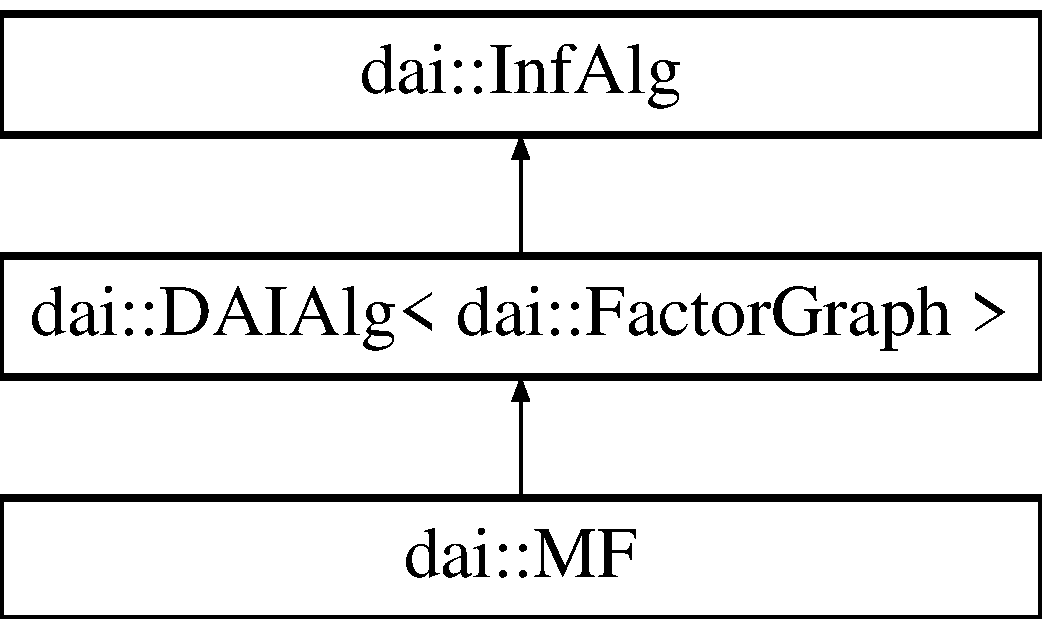
\includegraphics[height=3cm]{classdai_1_1MF}
\end{center}
\end{figure}


\subsection{Detailed Description}
Approximate inference algorithm \char`\"{}Mean Field\char`\"{}. \subsection*{Public Member Functions}
\begin{CompactItemize}
\item 
\hypertarget{classdai_1_1MF_2e40d786c9e8d34864fe09e1da56632c}{
\hyperlink{classdai_1_1MF_2e40d786c9e8d34864fe09e1da56632c}{MF} ()}
\label{classdai_1_1MF_2e40d786c9e8d34864fe09e1da56632c}

\begin{CompactList}\small\item\em Default constructor. \item\end{CompactList}\item 
\hypertarget{classdai_1_1MF_813ea21faea74d26067ac0876d2f89d6}{
\hyperlink{classdai_1_1MF_813ea21faea74d26067ac0876d2f89d6}{MF} (const \hyperlink{classdai_1_1MF}{MF} \&x)}
\label{classdai_1_1MF_813ea21faea74d26067ac0876d2f89d6}

\begin{CompactList}\small\item\em Copy constructor. \item\end{CompactList}\item 
\hypertarget{classdai_1_1MF_d8f30354060027fbb96f303947163dbc}{
\hyperlink{classdai_1_1MF}{MF} \& \hyperlink{classdai_1_1MF_d8f30354060027fbb96f303947163dbc}{operator=} (const \hyperlink{classdai_1_1MF}{MF} \&x)}
\label{classdai_1_1MF_d8f30354060027fbb96f303947163dbc}

\begin{CompactList}\small\item\em Assignment operator. \item\end{CompactList}\item 
\hypertarget{classdai_1_1MF_968fe2b9d9cc604a9d81c9ea15be8d72}{
\hyperlink{classdai_1_1MF_968fe2b9d9cc604a9d81c9ea15be8d72}{MF} (const \hyperlink{classdai_1_1FactorGraph}{FactorGraph} \&fg, const \hyperlink{classdai_1_1PropertySet}{PropertySet} \&opts)}
\label{classdai_1_1MF_968fe2b9d9cc604a9d81c9ea15be8d72}

\begin{CompactList}\small\item\em Construct from \hyperlink{classdai_1_1FactorGraph}{FactorGraph} fg and \hyperlink{classdai_1_1PropertySet}{PropertySet} opts. \item\end{CompactList}\item 
\hypertarget{classdai_1_1DAIAlg_48ba6a58d10b8802d690e5e92ec5abe9}{
void \hyperlink{classdai_1_1DAIAlg_48ba6a58d10b8802d690e5e92ec5abe9}{backupFactor} (size\_\-t I)}
\label{classdai_1_1DAIAlg_48ba6a58d10b8802d690e5e92ec5abe9}

\begin{CompactList}\small\item\em Save factor I. \item\end{CompactList}\item 
\hypertarget{classdai_1_1DAIAlg_0176904d3b4b9d083288ea8c4a2dc8bc}{
void \hyperlink{classdai_1_1DAIAlg_0176904d3b4b9d083288ea8c4a2dc8bc}{backupFactors} (const \hyperlink{classdai_1_1VarSet}{VarSet} \&ns)}
\label{classdai_1_1DAIAlg_0176904d3b4b9d083288ea8c4a2dc8bc}

\begin{CompactList}\small\item\em Save Factors involving ns. \item\end{CompactList}\item 
\hypertarget{classdai_1_1DAIAlg_bf8dbd2797ec871e86566a6dfc0864e3}{
void \hyperlink{classdai_1_1DAIAlg_bf8dbd2797ec871e86566a6dfc0864e3}{restoreFactor} (size\_\-t I)}
\label{classdai_1_1DAIAlg_bf8dbd2797ec871e86566a6dfc0864e3}

\begin{CompactList}\small\item\em Restore factor I. \item\end{CompactList}\item 
\hypertarget{classdai_1_1DAIAlg_3ce97e9370f1cdc785526c1a6c1eaadf}{
void \hyperlink{classdai_1_1DAIAlg_3ce97e9370f1cdc785526c1a6c1eaadf}{restoreFactors} (const \hyperlink{classdai_1_1VarSet}{VarSet} \&ns)}
\label{classdai_1_1DAIAlg_3ce97e9370f1cdc785526c1a6c1eaadf}

\begin{CompactList}\small\item\em Restore Factors involving ns. \item\end{CompactList}\item 
\hypertarget{classdai_1_1DAIAlg_b7d537f1a9d116617d8dce722ce65dc0}{
void \hyperlink{classdai_1_1DAIAlg_b7d537f1a9d116617d8dce722ce65dc0}{clamp} (const \hyperlink{classdai_1_1Var}{Var} \&n, size\_\-t i, bool backup=false)}
\label{classdai_1_1DAIAlg_b7d537f1a9d116617d8dce722ce65dc0}

\begin{CompactList}\small\item\em Clamp variable n to value i (i.e. multiply with a Kronecker delta $\delta_{x_n, i}$). \item\end{CompactList}\item 
\hypertarget{classdai_1_1DAIAlg_7f0b8452352080a1e35ab9a68cb589fd}{
void \hyperlink{classdai_1_1DAIAlg_7f0b8452352080a1e35ab9a68cb589fd}{makeCavity} (size\_\-t i, bool backup=false)}
\label{classdai_1_1DAIAlg_7f0b8452352080a1e35ab9a68cb589fd}

\begin{CompactList}\small\item\em Set all factors interacting with var(i) to 1. \item\end{CompactList}\item 
\hypertarget{classdai_1_1DAIAlg_9348542c22d04ed804388f1fe3009fa3}{
\hyperlink{classdai_1_1FactorGraph}{FactorGraph} \& \hyperlink{classdai_1_1DAIAlg_9348542c22d04ed804388f1fe3009fa3}{fg} ()}
\label{classdai_1_1DAIAlg_9348542c22d04ed804388f1fe3009fa3}

\begin{CompactList}\small\item\em Get reference to underlying \hyperlink{classdai_1_1FactorGraph}{FactorGraph}. \item\end{CompactList}\item 
\hypertarget{classdai_1_1DAIAlg_35400e471b8c3c98bef6c74ceac8fa16}{
const \hyperlink{classdai_1_1FactorGraph}{FactorGraph} \& \hyperlink{classdai_1_1DAIAlg_35400e471b8c3c98bef6c74ceac8fa16}{fg} () const }
\label{classdai_1_1DAIAlg_35400e471b8c3c98bef6c74ceac8fa16}

\begin{CompactList}\small\item\em Get const reference to underlying \hyperlink{classdai_1_1FactorGraph}{FactorGraph}. \item\end{CompactList}\end{CompactItemize}
\begin{Indent}{\bf General InfAlg interface}\par
\begin{CompactItemize}
\item 
\hypertarget{classdai_1_1MF_c209b5cd623a33d0d1b0041d0a7cdf10}{
virtual \hyperlink{classdai_1_1MF}{MF} $\ast$ \hyperlink{classdai_1_1MF_c209b5cd623a33d0d1b0041d0a7cdf10}{clone} () const }
\label{classdai_1_1MF_c209b5cd623a33d0d1b0041d0a7cdf10}

\begin{CompactList}\small\item\em Returns a pointer to a new, cloned copy of $\ast$this (i.e., virtual copy constructor). \item\end{CompactList}\item 
\hypertarget{classdai_1_1MF_d74dbcd156314d1b6072c80917847587}{
virtual \hyperlink{classdai_1_1MF}{MF} $\ast$ \hyperlink{classdai_1_1MF_d74dbcd156314d1b6072c80917847587}{create} () const }
\label{classdai_1_1MF_d74dbcd156314d1b6072c80917847587}

\begin{CompactList}\small\item\em Returns a pointer to a newly constructed object $\ast$this (i.e., virtual default constructor). \item\end{CompactList}\item 
\hypertarget{classdai_1_1MF_f4e80fe7390fbb3e2496b1056b05c5e4}{
virtual std::string \hyperlink{classdai_1_1MF_f4e80fe7390fbb3e2496b1056b05c5e4}{identify} () const }
\label{classdai_1_1MF_f4e80fe7390fbb3e2496b1056b05c5e4}

\begin{CompactList}\small\item\em Identifies itself for logging purposes. \item\end{CompactList}\item 
\hypertarget{classdai_1_1MF_cee4df06c59d8e6ab4663129d59b419e}{
virtual \hyperlink{classdai_1_1TFactor}{Factor} \hyperlink{classdai_1_1MF_cee4df06c59d8e6ab4663129d59b419e}{belief} (const \hyperlink{classdai_1_1Var}{Var} \&n) const }
\label{classdai_1_1MF_cee4df06c59d8e6ab4663129d59b419e}

\begin{CompactList}\small\item\em Returns the \char`\"{}belief\char`\"{} (i.e., approximate marginal probability distribution) of a variable. \item\end{CompactList}\item 
\hypertarget{classdai_1_1MF_704446500780ea4e2b834bb03cff0e24}{
virtual \hyperlink{classdai_1_1TFactor}{Factor} \hyperlink{classdai_1_1MF_704446500780ea4e2b834bb03cff0e24}{belief} (const \hyperlink{classdai_1_1VarSet}{VarSet} \&ns) const }
\label{classdai_1_1MF_704446500780ea4e2b834bb03cff0e24}

\begin{CompactList}\small\item\em Returns the \char`\"{}belief\char`\"{} (i.e., approximate marginal probability distribution) of a set of variables. \item\end{CompactList}\item 
\hypertarget{classdai_1_1MF_a6c307192d3b4141e2d1b0b46f3319a8}{
virtual std::vector$<$ \hyperlink{classdai_1_1TFactor}{Factor} $>$ \hyperlink{classdai_1_1MF_a6c307192d3b4141e2d1b0b46f3319a8}{beliefs} () const }
\label{classdai_1_1MF_a6c307192d3b4141e2d1b0b46f3319a8}

\begin{CompactList}\small\item\em Returns all \char`\"{}beliefs\char`\"{} (i.e., approximate marginal probability distribution) calculated by the algorithm. \item\end{CompactList}\item 
\hypertarget{classdai_1_1MF_ad8b559b72143257ca997bd5975a1d69}{
virtual \hyperlink{namespacedai_e7d0472fdc89a8635825d01940e91cbf}{Real} \hyperlink{classdai_1_1MF_ad8b559b72143257ca997bd5975a1d69}{logZ} () const }
\label{classdai_1_1MF_ad8b559b72143257ca997bd5975a1d69}

\begin{CompactList}\small\item\em Returns the logarithm of the (approximated) partition sum (normalizing constant of the factor graph). \item\end{CompactList}\item 
virtual void \hyperlink{classdai_1_1MF_eb993d502d0cb97424ebff82e0cf6839}{init} ()
\begin{CompactList}\small\item\em Initializes all data structures of the approximate inference algorithm. \item\end{CompactList}\item 
virtual void \hyperlink{classdai_1_1MF_49ddd5c9c9f51ee9fb5e153b7194ac71}{init} (const \hyperlink{classdai_1_1VarSet}{VarSet} \&ns)
\begin{CompactList}\small\item\em Initializes all data structures corresponding to some set of variables. \item\end{CompactList}\item 
\hypertarget{classdai_1_1MF_bd9d1de4bfb3fb538c9949a7c82d7984}{
virtual double \hyperlink{classdai_1_1MF_bd9d1de4bfb3fb538c9949a7c82d7984}{run} ()}
\label{classdai_1_1MF_bd9d1de4bfb3fb538c9949a7c82d7984}

\begin{CompactList}\small\item\em Runs the approximate inference algorithm. \item\end{CompactList}\item 
virtual double \hyperlink{classdai_1_1MF_032b149026f011a5cbcd01eb08a3b8dc}{maxDiff} () const 
\item 
virtual size\_\-t \hyperlink{classdai_1_1MF_e2daf3cd007572d19d6156f2484db4fd}{Iterations} () const 
\end{CompactItemize}
\end{Indent}
\begin{Indent}{\bf Additional interface specific for MF}\par
\begin{CompactItemize}
\item 
\hypertarget{classdai_1_1MF_b5f9fa5f11b2ec4377db1d1c1360cf86}{
\hyperlink{classdai_1_1TFactor}{Factor} \textbf{beliefV} (size\_\-t i) const }
\label{classdai_1_1MF_b5f9fa5f11b2ec4377db1d1c1360cf86}

\end{CompactItemize}
\end{Indent}
\subsection*{Public Attributes}
\begin{CompactItemize}
\item 
\hypertarget{classdai_1_1MF_7fe9b554132a55d416199fcea7da014c}{
struct \hyperlink{structdai_1_1MF_1_1Properties}{dai::MF::Properties} \hyperlink{classdai_1_1MF_7fe9b554132a55d416199fcea7da014c}{props}}
\label{classdai_1_1MF_7fe9b554132a55d416199fcea7da014c}

\begin{CompactList}\small\item\em Parameters of this inference algorithm. \item\end{CompactList}\end{CompactItemize}
\subsection*{Static Public Attributes}
\begin{CompactItemize}
\item 
\hypertarget{classdai_1_1MF_ad41c263042fe7c780d404b4b32574f8}{
static const char $\ast$ \hyperlink{classdai_1_1MF_ad41c263042fe7c780d404b4b32574f8}{Name} = \char`\"{}MF\char`\"{}}
\label{classdai_1_1MF_ad41c263042fe7c780d404b4b32574f8}

\begin{CompactList}\small\item\em Name of this inference algorithm. \item\end{CompactList}\end{CompactItemize}
\subsection*{Classes}
\begin{CompactItemize}
\item 
struct \hyperlink{structdai_1_1MF_1_1Properties}{Properties}
\begin{CompactList}\small\item\em Parameters of this inference algorithm. \item\end{CompactList}\end{CompactItemize}


\subsection{Member Function Documentation}
\hypertarget{classdai_1_1MF_eb993d502d0cb97424ebff82e0cf6839}{
\index{dai::MF@{dai::MF}!init@{init}}
\index{init@{init}!dai::MF@{dai::MF}}
\subsubsection[init]{\setlength{\rightskip}{0pt plus 5cm}void dai::MF::init ()\hspace{0.3cm}{\tt  \mbox{[}virtual\mbox{]}}}}
\label{classdai_1_1MF_eb993d502d0cb97424ebff82e0cf6839}


Initializes all data structures of the approximate inference algorithm. 

This method should be called at least once before \hyperlink{classdai_1_1MF_bd9d1de4bfb3fb538c9949a7c82d7984}{run()} is called 

Implements \hyperlink{classdai_1_1InfAlg_99dd53d1aaccf09a4b977a49a983cc85}{dai::InfAlg}.\hypertarget{classdai_1_1MF_49ddd5c9c9f51ee9fb5e153b7194ac71}{
\index{dai::MF@{dai::MF}!init@{init}}
\index{init@{init}!dai::MF@{dai::MF}}
\subsubsection[init]{\setlength{\rightskip}{0pt plus 5cm}void dai::MF::init (const {\bf VarSet} \& {\em ns})\hspace{0.3cm}{\tt  \mbox{[}virtual\mbox{]}}}}
\label{classdai_1_1MF_49ddd5c9c9f51ee9fb5e153b7194ac71}


Initializes all data structures corresponding to some set of variables. 

This method can be used to do a partial initialization after a part of the factor graph has changed. Instead of initializing all data structures, it only initializes those involving the variables in ns. 

Implements \hyperlink{classdai_1_1InfAlg_7d006e89e01a2f3e2a40b0f7f6e37ae5}{dai::InfAlg}.\hypertarget{classdai_1_1MF_032b149026f011a5cbcd01eb08a3b8dc}{
\index{dai::MF@{dai::MF}!maxDiff@{maxDiff}}
\index{maxDiff@{maxDiff}!dai::MF@{dai::MF}}
\subsubsection[maxDiff]{\setlength{\rightskip}{0pt plus 5cm}virtual double dai::MF::maxDiff () const\hspace{0.3cm}{\tt  \mbox{[}inline, virtual\mbox{]}}}}
\label{classdai_1_1MF_032b149026f011a5cbcd01eb08a3b8dc}


Return maximum difference between single node beliefs in the last pass \begin{Desc}
\item[Exceptions:]
\begin{description}
\item[{\em \hyperlink{classdai_1_1Exception}{Exception}}]if not implemented/supported \end{description}
\end{Desc}


Implements \hyperlink{classdai_1_1InfAlg_7e1ca7da15403d5d2af4a855186c0b46}{dai::InfAlg}.\hypertarget{classdai_1_1MF_e2daf3cd007572d19d6156f2484db4fd}{
\index{dai::MF@{dai::MF}!Iterations@{Iterations}}
\index{Iterations@{Iterations}!dai::MF@{dai::MF}}
\subsubsection[Iterations]{\setlength{\rightskip}{0pt plus 5cm}virtual size\_\-t dai::MF::Iterations () const\hspace{0.3cm}{\tt  \mbox{[}inline, virtual\mbox{]}}}}
\label{classdai_1_1MF_e2daf3cd007572d19d6156f2484db4fd}


Return number of passes over the factorgraph \begin{Desc}
\item[Exceptions:]
\begin{description}
\item[{\em \hyperlink{classdai_1_1Exception}{Exception}}]if not implemented/supported \end{description}
\end{Desc}


Implements \hyperlink{classdai_1_1InfAlg_7a93807863cc0a2025c1a78bdf1e14b8}{dai::InfAlg}.

The documentation for this class was generated from the following files:\begin{CompactItemize}
\item 
include/dai/\hyperlink{mf_8h}{mf.h}\item 
src/mf.cpp\end{CompactItemize}

\hypertarget{structdai_1_1MF_1_1Properties}{
\section{dai::MF::Properties Struct Reference}
\label{structdai_1_1MF_1_1Properties}\index{dai::MF::Properties@{dai::MF::Properties}}
}
{\tt \#include $<$dai/mf.h$>$}



\subsection{Detailed Description}
Parameters of this inference algorithm. \subsection*{Public Attributes}
\begin{CompactItemize}
\item 
\hypertarget{structdai_1_1MF_1_1Properties_3ec9f65a2ddfbae3b757c00c589a0777}{
size\_\-t \hyperlink{structdai_1_1MF_1_1Properties_3ec9f65a2ddfbae3b757c00c589a0777}{verbose}}
\label{structdai_1_1MF_1_1Properties_3ec9f65a2ddfbae3b757c00c589a0777}

\begin{CompactList}\small\item\em Verbosity. \item\end{CompactList}\item 
\hypertarget{structdai_1_1MF_1_1Properties_5818c3f97e389ce353ce791129a0d542}{
size\_\-t \hyperlink{structdai_1_1MF_1_1Properties_5818c3f97e389ce353ce791129a0d542}{maxiter}}
\label{structdai_1_1MF_1_1Properties_5818c3f97e389ce353ce791129a0d542}

\begin{CompactList}\small\item\em Maximum number of iterations. \item\end{CompactList}\item 
\hypertarget{structdai_1_1MF_1_1Properties_70d6b996d4e0f9327a6f6f23aafae953}{
double \hyperlink{structdai_1_1MF_1_1Properties_70d6b996d4e0f9327a6f6f23aafae953}{tol}}
\label{structdai_1_1MF_1_1Properties_70d6b996d4e0f9327a6f6f23aafae953}

\begin{CompactList}\small\item\em Tolerance. \item\end{CompactList}\item 
\hypertarget{structdai_1_1MF_1_1Properties_ba47da336eebca6bc7c066304ef47ab7}{
double \hyperlink{structdai_1_1MF_1_1Properties_ba47da336eebca6bc7c066304ef47ab7}{damping}}
\label{structdai_1_1MF_1_1Properties_ba47da336eebca6bc7c066304ef47ab7}

\begin{CompactList}\small\item\em Damping constant. \item\end{CompactList}\end{CompactItemize}


The documentation for this struct was generated from the following file:\begin{CompactItemize}
\item 
include/dai/\hyperlink{mf_8h}{mf.h}\end{CompactItemize}

\hypertarget{classdai_1_1MR}{
\section{dai::MR Class Reference}
\label{classdai_1_1MR}\index{dai::MR@{dai::MR}}
}
{\tt \#include $<$dai/mr.h$>$}

Inheritance diagram for dai::MR::\begin{figure}[H]
\begin{center}
\leavevmode
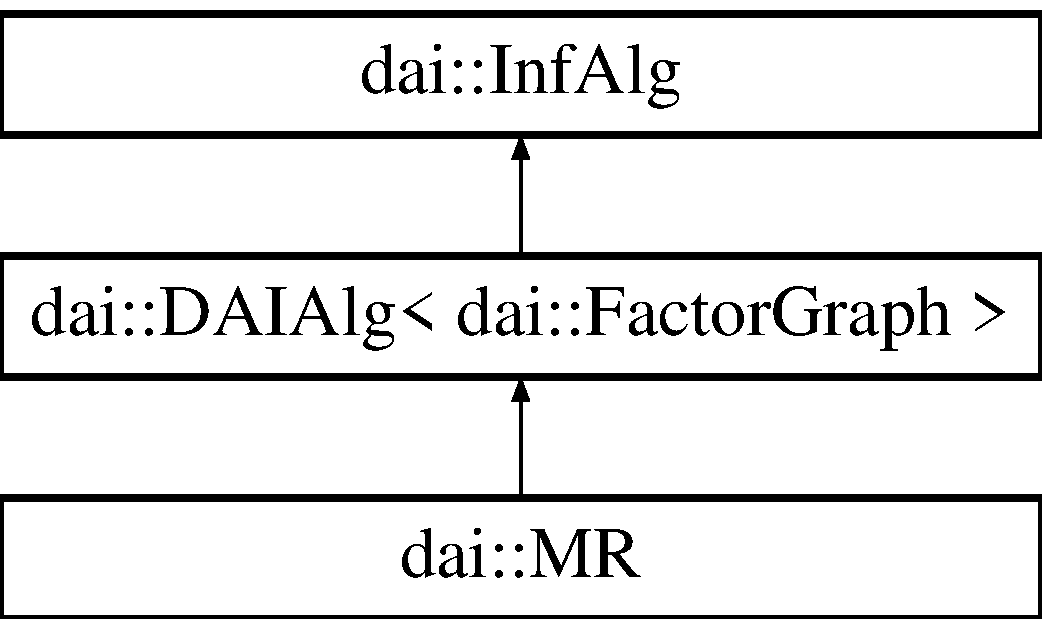
\includegraphics[height=3cm]{classdai_1_1MR}
\end{center}
\end{figure}


\subsection{Detailed Description}
Approximate inference algorithm by Montanari and Rizzo. \subsection*{Public Member Functions}
\begin{CompactItemize}
\item 
\hypertarget{classdai_1_1MR_0630645bffa9da4cb4df84e65d47ea7c}{
\hyperlink{classdai_1_1MR_0630645bffa9da4cb4df84e65d47ea7c}{MR} ()}
\label{classdai_1_1MR_0630645bffa9da4cb4df84e65d47ea7c}

\begin{CompactList}\small\item\em Default constructor. \item\end{CompactList}\item 
\hypertarget{classdai_1_1MR_81d8a3ad4ba4a373d4f1cfcf546b0576}{
\hyperlink{classdai_1_1MR_81d8a3ad4ba4a373d4f1cfcf546b0576}{MR} (const \hyperlink{classdai_1_1MR}{MR} \&x)}
\label{classdai_1_1MR_81d8a3ad4ba4a373d4f1cfcf546b0576}

\begin{CompactList}\small\item\em Copy constructor. \item\end{CompactList}\item 
\hypertarget{classdai_1_1MR_8a4884294fcb69eac8c201f3ddd2285d}{
\hyperlink{classdai_1_1MR}{MR} \& \hyperlink{classdai_1_1MR_8a4884294fcb69eac8c201f3ddd2285d}{operator=} (const \hyperlink{classdai_1_1MR}{MR} \&x)}
\label{classdai_1_1MR_8a4884294fcb69eac8c201f3ddd2285d}

\begin{CompactList}\small\item\em Assignment operator. \item\end{CompactList}\item 
\hypertarget{classdai_1_1MR_58f561154d9c74ac2f39a3b13196857f}{
\hyperlink{classdai_1_1MR_58f561154d9c74ac2f39a3b13196857f}{MR} (const \hyperlink{classdai_1_1FactorGraph}{FactorGraph} \&fg, const \hyperlink{classdai_1_1PropertySet}{PropertySet} \&opts)}
\label{classdai_1_1MR_58f561154d9c74ac2f39a3b13196857f}

\begin{CompactList}\small\item\em Construct from \hyperlink{classdai_1_1FactorGraph}{FactorGraph} fg and \hyperlink{classdai_1_1PropertySet}{PropertySet} opts. \item\end{CompactList}\item 
\hypertarget{classdai_1_1DAIAlg_48ba6a58d10b8802d690e5e92ec5abe9}{
void \hyperlink{classdai_1_1DAIAlg_48ba6a58d10b8802d690e5e92ec5abe9}{backupFactor} (size\_\-t I)}
\label{classdai_1_1DAIAlg_48ba6a58d10b8802d690e5e92ec5abe9}

\begin{CompactList}\small\item\em Save factor I. \item\end{CompactList}\item 
\hypertarget{classdai_1_1DAIAlg_0176904d3b4b9d083288ea8c4a2dc8bc}{
void \hyperlink{classdai_1_1DAIAlg_0176904d3b4b9d083288ea8c4a2dc8bc}{backupFactors} (const \hyperlink{classdai_1_1VarSet}{VarSet} \&ns)}
\label{classdai_1_1DAIAlg_0176904d3b4b9d083288ea8c4a2dc8bc}

\begin{CompactList}\small\item\em Save Factors involving ns. \item\end{CompactList}\item 
\hypertarget{classdai_1_1DAIAlg_bf8dbd2797ec871e86566a6dfc0864e3}{
void \hyperlink{classdai_1_1DAIAlg_bf8dbd2797ec871e86566a6dfc0864e3}{restoreFactor} (size\_\-t I)}
\label{classdai_1_1DAIAlg_bf8dbd2797ec871e86566a6dfc0864e3}

\begin{CompactList}\small\item\em Restore factor I. \item\end{CompactList}\item 
\hypertarget{classdai_1_1DAIAlg_3ce97e9370f1cdc785526c1a6c1eaadf}{
void \hyperlink{classdai_1_1DAIAlg_3ce97e9370f1cdc785526c1a6c1eaadf}{restoreFactors} (const \hyperlink{classdai_1_1VarSet}{VarSet} \&ns)}
\label{classdai_1_1DAIAlg_3ce97e9370f1cdc785526c1a6c1eaadf}

\begin{CompactList}\small\item\em Restore Factors involving ns. \item\end{CompactList}\item 
\hypertarget{classdai_1_1DAIAlg_b7d537f1a9d116617d8dce722ce65dc0}{
void \hyperlink{classdai_1_1DAIAlg_b7d537f1a9d116617d8dce722ce65dc0}{clamp} (const \hyperlink{classdai_1_1Var}{Var} \&n, size\_\-t i, bool backup=false)}
\label{classdai_1_1DAIAlg_b7d537f1a9d116617d8dce722ce65dc0}

\begin{CompactList}\small\item\em Clamp variable n to value i (i.e. multiply with a Kronecker delta $\delta_{x_n, i}$). \item\end{CompactList}\item 
\hypertarget{classdai_1_1DAIAlg_7f0b8452352080a1e35ab9a68cb589fd}{
void \hyperlink{classdai_1_1DAIAlg_7f0b8452352080a1e35ab9a68cb589fd}{makeCavity} (size\_\-t i, bool backup=false)}
\label{classdai_1_1DAIAlg_7f0b8452352080a1e35ab9a68cb589fd}

\begin{CompactList}\small\item\em Set all factors interacting with var(i) to 1. \item\end{CompactList}\item 
\hypertarget{classdai_1_1DAIAlg_9348542c22d04ed804388f1fe3009fa3}{
\hyperlink{classdai_1_1FactorGraph}{FactorGraph} \& \hyperlink{classdai_1_1DAIAlg_9348542c22d04ed804388f1fe3009fa3}{fg} ()}
\label{classdai_1_1DAIAlg_9348542c22d04ed804388f1fe3009fa3}

\begin{CompactList}\small\item\em Get reference to underlying \hyperlink{classdai_1_1FactorGraph}{FactorGraph}. \item\end{CompactList}\item 
\hypertarget{classdai_1_1DAIAlg_35400e471b8c3c98bef6c74ceac8fa16}{
const \hyperlink{classdai_1_1FactorGraph}{FactorGraph} \& \hyperlink{classdai_1_1DAIAlg_35400e471b8c3c98bef6c74ceac8fa16}{fg} () const }
\label{classdai_1_1DAIAlg_35400e471b8c3c98bef6c74ceac8fa16}

\begin{CompactList}\small\item\em Get const reference to underlying \hyperlink{classdai_1_1FactorGraph}{FactorGraph}. \item\end{CompactList}\end{CompactItemize}
\begin{Indent}{\bf General InfAlg interface}\par
\begin{CompactItemize}
\item 
\hypertarget{classdai_1_1MR_8d3a4cdd6c8b0643f419ac4af425a648}{
virtual \hyperlink{classdai_1_1MR}{MR} $\ast$ \hyperlink{classdai_1_1MR_8d3a4cdd6c8b0643f419ac4af425a648}{clone} () const }
\label{classdai_1_1MR_8d3a4cdd6c8b0643f419ac4af425a648}

\begin{CompactList}\small\item\em Returns a pointer to a new, cloned copy of $\ast$this (i.e., virtual copy constructor). \item\end{CompactList}\item 
\hypertarget{classdai_1_1MR_824091e73486b3ed5ece0586362dc030}{
virtual \hyperlink{classdai_1_1MR}{MR} $\ast$ \hyperlink{classdai_1_1MR_824091e73486b3ed5ece0586362dc030}{create} () const }
\label{classdai_1_1MR_824091e73486b3ed5ece0586362dc030}

\begin{CompactList}\small\item\em Returns a pointer to a newly constructed object $\ast$this (i.e., virtual default constructor). \item\end{CompactList}\item 
\hypertarget{classdai_1_1MR_8c05671b584167d78fd556d849be938b}{
virtual std::string \hyperlink{classdai_1_1MR_8c05671b584167d78fd556d849be938b}{identify} () const }
\label{classdai_1_1MR_8c05671b584167d78fd556d849be938b}

\begin{CompactList}\small\item\em Identifies itself for logging purposes. \item\end{CompactList}\item 
\hypertarget{classdai_1_1MR_264f15595ab0257931cbe1cf19838583}{
virtual \hyperlink{classdai_1_1TFactor}{Factor} \hyperlink{classdai_1_1MR_264f15595ab0257931cbe1cf19838583}{belief} (const \hyperlink{classdai_1_1Var}{Var} \&n) const }
\label{classdai_1_1MR_264f15595ab0257931cbe1cf19838583}

\begin{CompactList}\small\item\em Returns the \char`\"{}belief\char`\"{} (i.e., approximate marginal probability distribution) of a variable. \item\end{CompactList}\item 
\hypertarget{classdai_1_1MR_2b0bc5b3f3ddab92fd9029e4b21c6e04}{
virtual \hyperlink{classdai_1_1TFactor}{Factor} \hyperlink{classdai_1_1MR_2b0bc5b3f3ddab92fd9029e4b21c6e04}{belief} (const \hyperlink{classdai_1_1VarSet}{VarSet} \&) const }
\label{classdai_1_1MR_2b0bc5b3f3ddab92fd9029e4b21c6e04}

\begin{CompactList}\small\item\em Returns the \char`\"{}belief\char`\"{} (i.e., approximate marginal probability distribution) of a set of variables. \item\end{CompactList}\item 
\hypertarget{classdai_1_1MR_fdeba6c62b51ad80f13ac75bb7ffcfb5}{
virtual std::vector$<$ \hyperlink{classdai_1_1TFactor}{Factor} $>$ \hyperlink{classdai_1_1MR_fdeba6c62b51ad80f13ac75bb7ffcfb5}{beliefs} () const }
\label{classdai_1_1MR_fdeba6c62b51ad80f13ac75bb7ffcfb5}

\begin{CompactList}\small\item\em Returns all \char`\"{}beliefs\char`\"{} (i.e., approximate marginal probability distribution) calculated by the algorithm. \item\end{CompactList}\item 
\hypertarget{classdai_1_1MR_f1599e561432596af2d2b4ec423e0a8d}{
virtual \hyperlink{namespacedai_e7d0472fdc89a8635825d01940e91cbf}{Real} \hyperlink{classdai_1_1MR_f1599e561432596af2d2b4ec423e0a8d}{logZ} () const }
\label{classdai_1_1MR_f1599e561432596af2d2b4ec423e0a8d}

\begin{CompactList}\small\item\em Returns the logarithm of the (approximated) partition sum (normalizing constant of the factor graph). \item\end{CompactList}\item 
virtual void \hyperlink{classdai_1_1MR_859f5c780ec490232dc7a2b8f11da38b}{init} ()
\begin{CompactList}\small\item\em Initializes all data structures of the approximate inference algorithm. \item\end{CompactList}\item 
virtual void \hyperlink{classdai_1_1MR_da0e0829e87b541633dbb6078529c21d}{init} (const \hyperlink{classdai_1_1VarSet}{VarSet} \&)
\begin{CompactList}\small\item\em Initializes all data structures corresponding to some set of variables. \item\end{CompactList}\item 
\hypertarget{classdai_1_1MR_bc686f1fcd4b91c6592365db752c413e}{
virtual double \hyperlink{classdai_1_1MR_bc686f1fcd4b91c6592365db752c413e}{run} ()}
\label{classdai_1_1MR_bc686f1fcd4b91c6592365db752c413e}

\begin{CompactList}\small\item\em Runs the approximate inference algorithm. \item\end{CompactList}\item 
virtual double \hyperlink{classdai_1_1MR_a55d0a62912e9fe8a685157cfa309918}{maxDiff} () const 
\item 
virtual size\_\-t \hyperlink{classdai_1_1MR_6a199aa1d43b3c143a4b631735f53ee3}{Iterations} () const 
\end{CompactItemize}
\end{Indent}
\subsection*{Public Attributes}
\begin{CompactItemize}
\item 
\hypertarget{classdai_1_1MR_4d4ad4e50b277d36d33f3cdb86644fc0}{
struct \hyperlink{structdai_1_1MR_1_1Properties}{dai::MR::Properties} \hyperlink{classdai_1_1MR_4d4ad4e50b277d36d33f3cdb86644fc0}{props}}
\label{classdai_1_1MR_4d4ad4e50b277d36d33f3cdb86644fc0}

\begin{CompactList}\small\item\em Parameters of this inference algorithm. \item\end{CompactList}\end{CompactItemize}
\subsection*{Static Public Attributes}
\begin{CompactItemize}
\item 
\hypertarget{classdai_1_1MR_bc953e4a7a7d821f25e0ccbcdf8d304f}{
static const char $\ast$ \hyperlink{classdai_1_1MR_bc953e4a7a7d821f25e0ccbcdf8d304f}{Name} = \char`\"{}MR\char`\"{}}
\label{classdai_1_1MR_bc953e4a7a7d821f25e0ccbcdf8d304f}

\begin{CompactList}\small\item\em Name of this inference method. \item\end{CompactList}\end{CompactItemize}
\subsection*{Classes}
\begin{CompactItemize}
\item 
struct \hyperlink{structdai_1_1MR_1_1Properties}{Properties}
\begin{CompactList}\small\item\em Parameters of this inference algorithm. \item\end{CompactList}\end{CompactItemize}


\subsection{Member Function Documentation}
\hypertarget{classdai_1_1MR_859f5c780ec490232dc7a2b8f11da38b}{
\index{dai::MR@{dai::MR}!init@{init}}
\index{init@{init}!dai::MR@{dai::MR}}
\subsubsection[init]{\setlength{\rightskip}{0pt plus 5cm}virtual void dai::MR::init ()\hspace{0.3cm}{\tt  \mbox{[}inline, virtual\mbox{]}}}}
\label{classdai_1_1MR_859f5c780ec490232dc7a2b8f11da38b}


Initializes all data structures of the approximate inference algorithm. 

This method should be called at least once before \hyperlink{classdai_1_1MR_bc686f1fcd4b91c6592365db752c413e}{run()} is called 

Implements \hyperlink{classdai_1_1InfAlg_99dd53d1aaccf09a4b977a49a983cc85}{dai::InfAlg}.\hypertarget{classdai_1_1MR_da0e0829e87b541633dbb6078529c21d}{
\index{dai::MR@{dai::MR}!init@{init}}
\index{init@{init}!dai::MR@{dai::MR}}
\subsubsection[init]{\setlength{\rightskip}{0pt plus 5cm}virtual void dai::MR::init (const {\bf VarSet} \& {\em ns})\hspace{0.3cm}{\tt  \mbox{[}inline, virtual\mbox{]}}}}
\label{classdai_1_1MR_da0e0829e87b541633dbb6078529c21d}


Initializes all data structures corresponding to some set of variables. 

This method can be used to do a partial initialization after a part of the factor graph has changed. Instead of initializing all data structures, it only initializes those involving the variables in ns. 

Implements \hyperlink{classdai_1_1InfAlg_7d006e89e01a2f3e2a40b0f7f6e37ae5}{dai::InfAlg}.\hypertarget{classdai_1_1MR_a55d0a62912e9fe8a685157cfa309918}{
\index{dai::MR@{dai::MR}!maxDiff@{maxDiff}}
\index{maxDiff@{maxDiff}!dai::MR@{dai::MR}}
\subsubsection[maxDiff]{\setlength{\rightskip}{0pt plus 5cm}virtual double dai::MR::maxDiff () const\hspace{0.3cm}{\tt  \mbox{[}inline, virtual\mbox{]}}}}
\label{classdai_1_1MR_a55d0a62912e9fe8a685157cfa309918}


Return maximum difference between single node beliefs in the last pass \begin{Desc}
\item[Exceptions:]
\begin{description}
\item[{\em \hyperlink{classdai_1_1Exception}{Exception}}]if not implemented/supported \end{description}
\end{Desc}


Implements \hyperlink{classdai_1_1InfAlg_7e1ca7da15403d5d2af4a855186c0b46}{dai::InfAlg}.\hypertarget{classdai_1_1MR_6a199aa1d43b3c143a4b631735f53ee3}{
\index{dai::MR@{dai::MR}!Iterations@{Iterations}}
\index{Iterations@{Iterations}!dai::MR@{dai::MR}}
\subsubsection[Iterations]{\setlength{\rightskip}{0pt plus 5cm}virtual size\_\-t dai::MR::Iterations () const\hspace{0.3cm}{\tt  \mbox{[}inline, virtual\mbox{]}}}}
\label{classdai_1_1MR_6a199aa1d43b3c143a4b631735f53ee3}


Return number of passes over the factorgraph \begin{Desc}
\item[Exceptions:]
\begin{description}
\item[{\em \hyperlink{classdai_1_1Exception}{Exception}}]if not implemented/supported \end{description}
\end{Desc}


Implements \hyperlink{classdai_1_1InfAlg_7a93807863cc0a2025c1a78bdf1e14b8}{dai::InfAlg}.

The documentation for this class was generated from the following files:\begin{CompactItemize}
\item 
include/dai/\hyperlink{mr_8h}{mr.h}\item 
src/mr.cpp\end{CompactItemize}

\hypertarget{structdai_1_1MR_1_1Properties}{
\section{dai::MR::Properties Struct Reference}
\label{structdai_1_1MR_1_1Properties}\index{dai::MR::Properties@{dai::MR::Properties}}
}
{\tt \#include $<$dai/mr.h$>$}



\subsection{Detailed Description}
Parameters of this inference algorithm. \subsection*{Public Attributes}
\begin{CompactItemize}
\item 
size\_\-t \hyperlink{structdai_1_1MR_1_1Properties_e0281396e1ee677e1b6ae15f9ae67f99}{verbose}
\begin{CompactList}\small\item\em Enumeration of different types of update equations. \item\end{CompactList}\item 
\hypertarget{structdai_1_1MR_1_1Properties_94665674b559c260c67d45688b829bfe}{
double \hyperlink{structdai_1_1MR_1_1Properties_94665674b559c260c67d45688b829bfe}{tol}}
\label{structdai_1_1MR_1_1Properties_94665674b559c260c67d45688b829bfe}

\begin{CompactList}\small\item\em Tolerance. \item\end{CompactList}\item 
\hypertarget{structdai_1_1MR_1_1Properties_f1e2899da2779d1b0d7640f87d899f17}{
UpdateType \hyperlink{structdai_1_1MR_1_1Properties_f1e2899da2779d1b0d7640f87d899f17}{updates}}
\label{structdai_1_1MR_1_1Properties_f1e2899da2779d1b0d7640f87d899f17}

\begin{CompactList}\small\item\em Update equations. \item\end{CompactList}\item 
\hypertarget{structdai_1_1MR_1_1Properties_5c400e8635d85478270d653a8a7f351b}{
InitType \hyperlink{structdai_1_1MR_1_1Properties_5c400e8635d85478270d653a8a7f351b}{inits}}
\label{structdai_1_1MR_1_1Properties_5c400e8635d85478270d653a8a7f351b}

\begin{CompactList}\small\item\em How to initialize the cavity correlations. \item\end{CompactList}\end{CompactItemize}


\subsection{Member Data Documentation}
\hypertarget{structdai_1_1MR_1_1Properties_e0281396e1ee677e1b6ae15f9ae67f99}{
\index{dai::MR::Properties@{dai::MR::Properties}!verbose@{verbose}}
\index{verbose@{verbose}!dai::MR::Properties@{dai::MR::Properties}}
\subsubsection[verbose]{\setlength{\rightskip}{0pt plus 5cm}size\_\-t {\bf dai::MR::Properties::verbose}}}
\label{structdai_1_1MR_1_1Properties_e0281396e1ee677e1b6ae15f9ae67f99}


Enumeration of different types of update equations. 

Enumeration of different ways of initializing the cavity correlations Verbosity 

The documentation for this struct was generated from the following file:\begin{CompactItemize}
\item 
include/dai/\hyperlink{mr_8h}{mr.h}\end{CompactItemize}

\hypertarget{classdai_1_1MultiFor}{
\section{dai::MultiFor Class Reference}
\label{classdai_1_1MultiFor}\index{dai::MultiFor@{dai::MultiFor}}
}
{\tt \#include $<$dai/index.h$>$}



\subsection{Detailed Description}
\hyperlink{classdai_1_1MultiFor}{MultiFor} makes it easy to perform a dynamic number of nested for loops. 

An example of the usage is as follows: 

\begin{Code}\begin{verbatim}  std::vector<size_t> dims;
  dims.push_back( 3 );
  dims.push_back( 4 );
  dims.push_back( 5 );
  for( MultiFor s(dims); s.valid(); ++s )
      cout << "linear index: " << (size_t)s << " corresponds to indices " << s[0] << ", " << s[1] << ", " << s[2] << endl;
\end{verbatim}
\end{Code}

 which would be equivalent to: 

\begin{Code}\begin{verbatim}  size_t s = 0;
  for( size_t s0 = 0; s0 < 3; s0++ )
      for( size_t s1 = 0; s1 < 4; s1++ )
          for( size_t s2 = 0; s2 < 5; s++, s2++ )
              cout << "linear index: " << (size_t)s << " corresponds to indices " << s0 << ", " << s1 << ", " << s2 << endl;
\end{verbatim}
\end{Code}

 \subsection*{Public Member Functions}
\begin{CompactItemize}
\item 
\hypertarget{classdai_1_1MultiFor_9ad4786f54d6cebf5bc6111058415c79}{
\hyperlink{classdai_1_1MultiFor_9ad4786f54d6cebf5bc6111058415c79}{MultiFor} ()}
\label{classdai_1_1MultiFor_9ad4786f54d6cebf5bc6111058415c79}

\begin{CompactList}\small\item\em Default constructor. \item\end{CompactList}\item 
\hypertarget{classdai_1_1MultiFor_6f3ee9f121903fa4fddf56416151e3c0}{
\hyperlink{classdai_1_1MultiFor_6f3ee9f121903fa4fddf56416151e3c0}{MultiFor} (const std::vector$<$ size\_\-t $>$ \&d)}
\label{classdai_1_1MultiFor_6f3ee9f121903fa4fddf56416151e3c0}

\begin{CompactList}\small\item\em Initialize from vector of index dimensions. \item\end{CompactList}\item 
\hypertarget{classdai_1_1MultiFor_f29ba6cf5f64475130f5c48fd4b52e53}{
\hyperlink{classdai_1_1MultiFor_f29ba6cf5f64475130f5c48fd4b52e53}{MultiFor} (const \hyperlink{classdai_1_1MultiFor}{MultiFor} \&x)}
\label{classdai_1_1MultiFor_f29ba6cf5f64475130f5c48fd4b52e53}

\begin{CompactList}\small\item\em Copy constructor. \item\end{CompactList}\item 
\hypertarget{classdai_1_1MultiFor_0f5bb0cd496a84c7705a95cd52b80096}{
\hyperlink{classdai_1_1MultiFor}{MultiFor} \& \hyperlink{classdai_1_1MultiFor_0f5bb0cd496a84c7705a95cd52b80096}{operator=} (const \hyperlink{classdai_1_1MultiFor}{MultiFor} \&x)}
\label{classdai_1_1MultiFor_0f5bb0cd496a84c7705a95cd52b80096}

\begin{CompactList}\small\item\em Assignment operator. \item\end{CompactList}\item 
\hypertarget{classdai_1_1MultiFor_3127a6180e9d1ade8e4e0a310d46c964}{
\hyperlink{classdai_1_1MultiFor_3127a6180e9d1ade8e4e0a310d46c964}{operator size\_\-t} () const }
\label{classdai_1_1MultiFor_3127a6180e9d1ade8e4e0a310d46c964}

\begin{CompactList}\small\item\em Return linear state. \item\end{CompactList}\item 
\hypertarget{classdai_1_1MultiFor_dcf44dd24e2be73381cf3b5cdbe470a1}{
size\_\-t \hyperlink{classdai_1_1MultiFor_dcf44dd24e2be73381cf3b5cdbe470a1}{operator\mbox{[}$\,$\mbox{]}} (size\_\-t k) const }
\label{classdai_1_1MultiFor_dcf44dd24e2be73381cf3b5cdbe470a1}

\begin{CompactList}\small\item\em Return k'th index. \item\end{CompactList}\item 
\hypertarget{classdai_1_1MultiFor_ca071de84757bdc9b45982e9826a1fdb}{
\hyperlink{classdai_1_1MultiFor}{MultiFor} \& \hyperlink{classdai_1_1MultiFor_ca071de84757bdc9b45982e9826a1fdb}{operator++} ()}
\label{classdai_1_1MultiFor_ca071de84757bdc9b45982e9826a1fdb}

\begin{CompactList}\small\item\em Prefix increment operator. \item\end{CompactList}\item 
\hypertarget{classdai_1_1MultiFor_06238b80d9f59dd6e56b516db39bdace}{
void \hyperlink{classdai_1_1MultiFor_06238b80d9f59dd6e56b516db39bdace}{operator++} (int)}
\label{classdai_1_1MultiFor_06238b80d9f59dd6e56b516db39bdace}

\begin{CompactList}\small\item\em Postfix increment operator. \item\end{CompactList}\item 
\hypertarget{classdai_1_1MultiFor_298bca4ac1b10613d2d2b7edd641c0a9}{
bool \hyperlink{classdai_1_1MultiFor_298bca4ac1b10613d2d2b7edd641c0a9}{valid} () const }
\label{classdai_1_1MultiFor_298bca4ac1b10613d2d2b7edd641c0a9}

\begin{CompactList}\small\item\em Returns true if the current state is valid. \item\end{CompactList}\end{CompactItemize}


The documentation for this class was generated from the following file:\begin{CompactItemize}
\item 
include/dai/\hyperlink{index_8h}{index.h}\end{CompactItemize}

\hypertarget{classdai_1_1Permute}{
\section{dai::Permute Class Reference}
\label{classdai_1_1Permute}\index{dai::Permute@{dai::Permute}}
}
{\tt \#include $<$dai/index.h$>$}



\subsection{Detailed Description}
Tool for calculating permutations of multiple indices. \subsection*{Public Member Functions}
\begin{CompactItemize}
\item 
\hypertarget{classdai_1_1Permute_138f021554272c9601e4cf6a25e6f62b}{
\hyperlink{classdai_1_1Permute_138f021554272c9601e4cf6a25e6f62b}{Permute} ()}
\label{classdai_1_1Permute_138f021554272c9601e4cf6a25e6f62b}

\begin{CompactList}\small\item\em Default constructor. \item\end{CompactList}\item 
\hypertarget{classdai_1_1Permute_d1af25b04480a33721e2f56e88cb0e25}{
\hyperlink{classdai_1_1Permute_d1af25b04480a33721e2f56e88cb0e25}{Permute} (const std::vector$<$ size\_\-t $>$ \&d, const std::vector$<$ size\_\-t $>$ \&sigma)}
\label{classdai_1_1Permute_d1af25b04480a33721e2f56e88cb0e25}

\begin{CompactList}\small\item\em Initialize from vector of index dimensions and permutation sigma. \item\end{CompactList}\item 
\hypertarget{classdai_1_1Permute_39b079d34fee292434e15faf136fd506}{
\hyperlink{classdai_1_1Permute_39b079d34fee292434e15faf136fd506}{Permute} (const \hyperlink{classdai_1_1Permute}{Permute} \&x)}
\label{classdai_1_1Permute_39b079d34fee292434e15faf136fd506}

\begin{CompactList}\small\item\em Copy constructor. \item\end{CompactList}\item 
\hypertarget{classdai_1_1Permute_99e896b039f3b9f6b737ccecba7dfdb5}{
\hyperlink{classdai_1_1Permute}{Permute} \& \hyperlink{classdai_1_1Permute_99e896b039f3b9f6b737ccecba7dfdb5}{operator=} (const \hyperlink{classdai_1_1Permute}{Permute} \&x)}
\label{classdai_1_1Permute_99e896b039f3b9f6b737ccecba7dfdb5}

\begin{CompactList}\small\item\em Assignment operator. \item\end{CompactList}\item 
size\_\-t \hyperlink{classdai_1_1Permute_19b7ca5bdbac54ba1a812ab52e6f11aa}{convert\_\-linear\_\-index} (size\_\-t li)
\end{CompactItemize}


\subsection{Member Function Documentation}
\hypertarget{classdai_1_1Permute_19b7ca5bdbac54ba1a812ab52e6f11aa}{
\index{dai::Permute@{dai::Permute}!convert\_\-linear\_\-index@{convert\_\-linear\_\-index}}
\index{convert\_\-linear\_\-index@{convert\_\-linear\_\-index}!dai::Permute@{dai::Permute}}
\subsubsection[convert\_\-linear\_\-index]{\setlength{\rightskip}{0pt plus 5cm}size\_\-t dai::Permute::convert\_\-linear\_\-index (size\_\-t {\em li})\hspace{0.3cm}{\tt  \mbox{[}inline\mbox{]}}}}
\label{classdai_1_1Permute_19b7ca5bdbac54ba1a812ab52e6f11aa}


Converts the linear index li to a vector index corresponding with the dimensions in \_\-dims, permutes it according to sigma, and converts it back to a linear index according to the permuted dimensions. 

The documentation for this class was generated from the following file:\begin{CompactItemize}
\item 
include/dai/\hyperlink{index_8h}{index.h}\end{CompactItemize}

\hypertarget{classdai_1_1PropertySet}{
\section{dai::PropertySet Class Reference}
\label{classdai_1_1PropertySet}\index{dai::PropertySet@{dai::PropertySet}}
}
{\tt \#include $<$dai/properties.h$>$}

Inherits std::map$<$ std::string, boost::any $>$.



\subsection{Detailed Description}
Represents a set of properties, mapping keys (of type PropertyKey) to values (of type PropertyValue). \subsection*{Public Member Functions}
\begin{CompactItemize}
\item 
\hypertarget{classdai_1_1PropertySet_cdc6cbd296f457d4a21d5795c62e8e8a}{
const \hyperlink{namespacedai_eb056b768d73d02c5796c4012f4170c7}{PropertyValue} \& \hyperlink{classdai_1_1PropertySet_cdc6cbd296f457d4a21d5795c62e8e8a}{Get} (const \hyperlink{namespacedai_cc877a85f4f4dbb6a0d58c434bb2b996}{PropertyKey} \&key) const }
\label{classdai_1_1PropertySet_cdc6cbd296f457d4a21d5795c62e8e8a}

\begin{CompactList}\small\item\em Gets a property. \item\end{CompactList}\item 
\hypertarget{classdai_1_1PropertySet_c5e6bb10fcbcbe1302494cd995e412df}{
\hyperlink{classdai_1_1PropertySet}{PropertySet} \& \hyperlink{classdai_1_1PropertySet_c5e6bb10fcbcbe1302494cd995e412df}{Set} (const \hyperlink{namespacedai_cc877a85f4f4dbb6a0d58c434bb2b996}{PropertyKey} \&key, const \hyperlink{namespacedai_eb056b768d73d02c5796c4012f4170c7}{PropertyValue} \&val)}
\label{classdai_1_1PropertySet_c5e6bb10fcbcbe1302494cd995e412df}

\begin{CompactList}\small\item\em Sets a property. \item\end{CompactList}\item 
\hypertarget{classdai_1_1PropertySet_1458c0be9e07b400b4e54df72dae6a3a}{
{\footnotesize template$<$typename ValueType$>$ }\\ValueType \hyperlink{classdai_1_1PropertySet_1458c0be9e07b400b4e54df72dae6a3a}{GetAs} (const \hyperlink{namespacedai_cc877a85f4f4dbb6a0d58c434bb2b996}{PropertyKey} \&key) const }
\label{classdai_1_1PropertySet_1458c0be9e07b400b4e54df72dae6a3a}

\begin{CompactList}\small\item\em Gets a property, casted as ValueType. \item\end{CompactList}\item 
\hypertarget{classdai_1_1PropertySet_0a18aa933d4b58c043e39f79a8870862}{
{\footnotesize template$<$typename ValueType$>$ }\\void \hyperlink{classdai_1_1PropertySet_0a18aa933d4b58c043e39f79a8870862}{ConvertTo} (const \hyperlink{namespacedai_cc877a85f4f4dbb6a0d58c434bb2b996}{PropertyKey} \&key)}
\label{classdai_1_1PropertySet_0a18aa933d4b58c043e39f79a8870862}

\begin{CompactList}\small\item\em Converts a property from string to ValueType (if necessary). \item\end{CompactList}\item 
\hypertarget{classdai_1_1PropertySet_8d8bebf882f713af015ffb02a563db60}{
{\footnotesize template$<$typename ValueType$>$ }\\ValueType \hyperlink{classdai_1_1PropertySet_8d8bebf882f713af015ffb02a563db60}{getStringAs} (const \hyperlink{namespacedai_cc877a85f4f4dbb6a0d58c434bb2b996}{PropertyKey} \&key) const }
\label{classdai_1_1PropertySet_8d8bebf882f713af015ffb02a563db60}

\begin{CompactList}\small\item\em Converts a property from string to ValueType (if necessary). \item\end{CompactList}\item 
\hypertarget{classdai_1_1PropertySet_8febf05009938e2cee9988a93b8a1d56}{
{\footnotesize template$<$typename ValueType$>$ }\\\hyperlink{classdai_1_1PropertySet}{PropertySet} \& \hyperlink{classdai_1_1PropertySet_8febf05009938e2cee9988a93b8a1d56}{setAsString} (const \hyperlink{namespacedai_cc877a85f4f4dbb6a0d58c434bb2b996}{PropertyKey} \&key, ValueType \&val)}
\label{classdai_1_1PropertySet_8febf05009938e2cee9988a93b8a1d56}

\begin{CompactList}\small\item\em Converts a property from ValueType to string (if necessary). \item\end{CompactList}\item 
\hypertarget{classdai_1_1PropertySet_51bfe57cacf9f79e788c490ed369869e}{
\hyperlink{classdai_1_1PropertySet}{PropertySet} \hyperlink{classdai_1_1PropertySet_51bfe57cacf9f79e788c490ed369869e}{operator()} (const \hyperlink{namespacedai_cc877a85f4f4dbb6a0d58c434bb2b996}{PropertyKey} \&key, const \hyperlink{namespacedai_eb056b768d73d02c5796c4012f4170c7}{PropertyValue} \&val) const }
\label{classdai_1_1PropertySet_51bfe57cacf9f79e788c490ed369869e}

\begin{CompactList}\small\item\em Shorthand for (temporarily) adding properties, e.g. \hyperlink{classdai_1_1PropertySet}{PropertySet} p()(\char`\"{}method\char`\"{},\char`\"{}BP\char`\"{})(\char`\"{}verbose\char`\"{},1)(\char`\"{}tol\char`\"{},1e-9). \item\end{CompactList}\item 
\hypertarget{classdai_1_1PropertySet_bc3df170db0dbba57cb11e3ef87f5948}{
bool \hyperlink{classdai_1_1PropertySet_bc3df170db0dbba57cb11e3ef87f5948}{hasKey} (const \hyperlink{namespacedai_cc877a85f4f4dbb6a0d58c434bb2b996}{PropertyKey} \&key) const }
\label{classdai_1_1PropertySet_bc3df170db0dbba57cb11e3ef87f5948}

\begin{CompactList}\small\item\em Check if a property with the given key exists. \item\end{CompactList}\end{CompactItemize}
\subsection*{Friends}
\begin{CompactItemize}
\item 
\hypertarget{classdai_1_1PropertySet_55c10d86bc897277108b545f22e06fb7}{
std::ostream \& \hyperlink{classdai_1_1PropertySet_55c10d86bc897277108b545f22e06fb7}{operator$<$$<$} (std::ostream \&os, const \hyperlink{classdai_1_1PropertySet}{PropertySet} \&ps)}
\label{classdai_1_1PropertySet_55c10d86bc897277108b545f22e06fb7}

\begin{CompactList}\small\item\em Writes a \hyperlink{classdai_1_1PropertySet}{PropertySet} object to an output stream. \item\end{CompactList}\item 
\hypertarget{classdai_1_1PropertySet_0ec4068ab9fe8a5690f560a2e7d778fc}{
std::istream \& \hyperlink{classdai_1_1PropertySet_0ec4068ab9fe8a5690f560a2e7d778fc}{operator$>$$>$} (std::istream \&is, \hyperlink{classdai_1_1PropertySet}{PropertySet} \&ps)}
\label{classdai_1_1PropertySet_0ec4068ab9fe8a5690f560a2e7d778fc}

\begin{CompactList}\small\item\em Reads a \hyperlink{classdai_1_1PropertySet}{PropertySet} object from an input stream, storing values as strings. \item\end{CompactList}\end{CompactItemize}


The documentation for this class was generated from the following file:\begin{CompactItemize}
\item 
include/dai/\hyperlink{properties_8h}{properties.h}\end{CompactItemize}

\hypertarget{classdai_1_1Region}{
\section{dai::Region Class Reference}
\label{classdai_1_1Region}\index{dai::Region@{dai::Region}}
}
{\tt \#include $<$dai/regiongraph.h$>$}

Inheritance diagram for dai::Region::\begin{figure}[H]
\begin{center}
\leavevmode
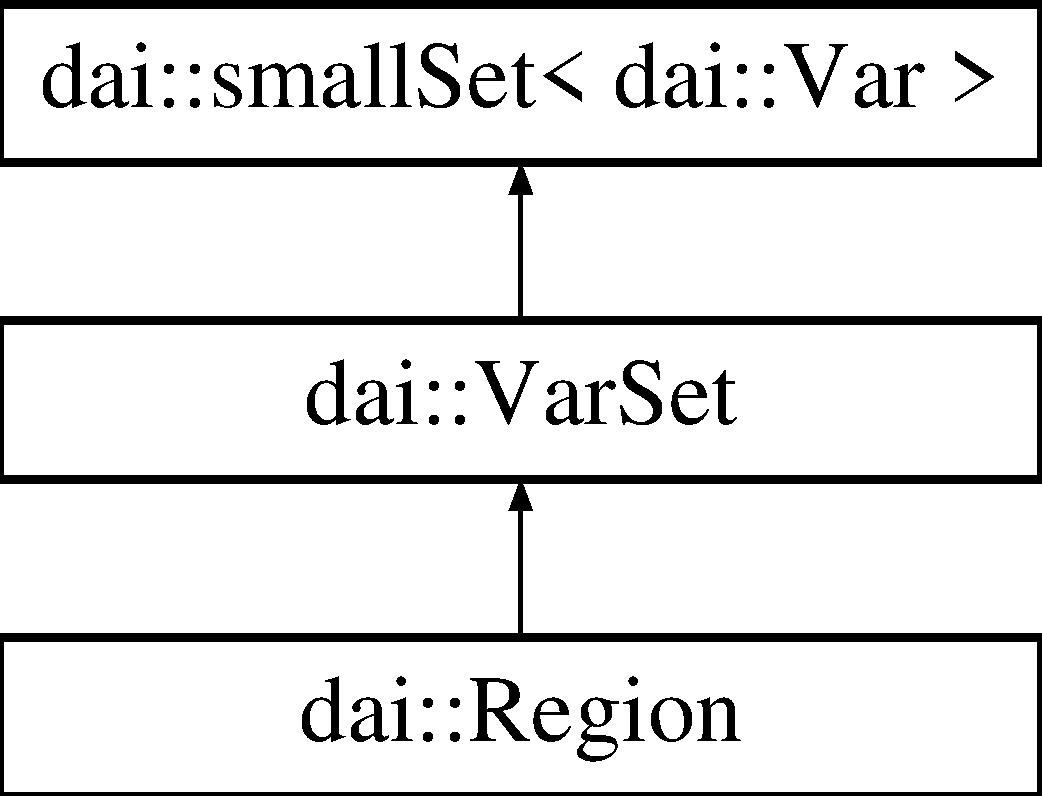
\includegraphics[height=3cm]{classdai_1_1Region}
\end{center}
\end{figure}


\subsection{Detailed Description}
A \hyperlink{classdai_1_1Region}{Region} is a set of variables with a counting number. \subsection*{Public Types}
\begin{CompactItemize}
\item 
\hypertarget{classdai_1_1smallSet_103c819872818d14a7234a1f618a815c}{
typedef std::vector$<$ T $>$::\hyperlink{classdai_1_1smallSet_103c819872818d14a7234a1f618a815c}{const\_\-iterator} \hyperlink{classdai_1_1smallSet_103c819872818d14a7234a1f618a815c}{const\_\-iterator}}
\label{classdai_1_1smallSet_103c819872818d14a7234a1f618a815c}

\begin{CompactList}\small\item\em Constant iterator over the elements. \item\end{CompactList}\item 
\hypertarget{classdai_1_1smallSet_254dd4f8cad9c7bce5522e9dbcfc4f49}{
typedef std::vector$<$ T $>$::\hyperlink{classdai_1_1smallSet_254dd4f8cad9c7bce5522e9dbcfc4f49}{iterator} \hyperlink{classdai_1_1smallSet_254dd4f8cad9c7bce5522e9dbcfc4f49}{iterator}}
\label{classdai_1_1smallSet_254dd4f8cad9c7bce5522e9dbcfc4f49}

\begin{CompactList}\small\item\em Iterator over the elements. \item\end{CompactList}\item 
\hypertarget{classdai_1_1smallSet_46882a9010267d41f447feb6aaf65cc1}{
typedef std::vector$<$ T $>$::\hyperlink{classdai_1_1smallSet_46882a9010267d41f447feb6aaf65cc1}{const\_\-reverse\_\-iterator} \hyperlink{classdai_1_1smallSet_46882a9010267d41f447feb6aaf65cc1}{const\_\-reverse\_\-iterator}}
\label{classdai_1_1smallSet_46882a9010267d41f447feb6aaf65cc1}

\begin{CompactList}\small\item\em Constant reverse iterator over the elements. \item\end{CompactList}\item 
\hypertarget{classdai_1_1smallSet_6dea3ee0aa40c4312e6278a7d17f516d}{
typedef std::vector$<$ T $>$::\hyperlink{classdai_1_1smallSet_6dea3ee0aa40c4312e6278a7d17f516d}{reverse\_\-iterator} \hyperlink{classdai_1_1smallSet_6dea3ee0aa40c4312e6278a7d17f516d}{reverse\_\-iterator}}
\label{classdai_1_1smallSet_6dea3ee0aa40c4312e6278a7d17f516d}

\begin{CompactList}\small\item\em Reverse iterator over the elements. \item\end{CompactList}\end{CompactItemize}
\subsection*{Public Member Functions}
\begin{CompactItemize}
\item 
\hypertarget{classdai_1_1Region_a27111b83697a921dea2e6bb3ecb0222}{
\hyperlink{classdai_1_1Region_a27111b83697a921dea2e6bb3ecb0222}{Region} ()}
\label{classdai_1_1Region_a27111b83697a921dea2e6bb3ecb0222}

\begin{CompactList}\small\item\em Default constructor. \item\end{CompactList}\item 
\hypertarget{classdai_1_1Region_c34eb5c18da857db32b1b9154c5becd3}{
\hyperlink{classdai_1_1Region_c34eb5c18da857db32b1b9154c5becd3}{Region} (const \hyperlink{classdai_1_1VarSet}{VarSet} \&x, double c)}
\label{classdai_1_1Region_c34eb5c18da857db32b1b9154c5becd3}

\begin{CompactList}\small\item\em Construct \hyperlink{classdai_1_1Region}{Region} from a \hyperlink{classdai_1_1VarSet}{VarSet} and a counting number. \item\end{CompactList}\item 
\hypertarget{classdai_1_1Region_b656a0703493a71decd4cdd2644f2d3e}{
\hyperlink{classdai_1_1Region_b656a0703493a71decd4cdd2644f2d3e}{Region} (const \hyperlink{classdai_1_1Region}{Region} \&x)}
\label{classdai_1_1Region_b656a0703493a71decd4cdd2644f2d3e}

\begin{CompactList}\small\item\em Copy constructor. \item\end{CompactList}\item 
\hypertarget{classdai_1_1Region_cd6f39ea63fec1c7bff3705ca8f0b82d}{
\hyperlink{classdai_1_1Region}{Region} \& \hyperlink{classdai_1_1Region_cd6f39ea63fec1c7bff3705ca8f0b82d}{operator=} (const \hyperlink{classdai_1_1Region}{Region} \&x)}
\label{classdai_1_1Region_cd6f39ea63fec1c7bff3705ca8f0b82d}

\begin{CompactList}\small\item\em Assignment operator. \item\end{CompactList}\item 
\hypertarget{classdai_1_1Region_5364578c485508d3fff986545c378877}{
const double \& \hyperlink{classdai_1_1Region_5364578c485508d3fff986545c378877}{c} () const }
\label{classdai_1_1Region_5364578c485508d3fff986545c378877}

\begin{CompactList}\small\item\em Provide read access to counting number. \item\end{CompactList}\item 
\hypertarget{classdai_1_1Region_d4ec2f311244ec4290496505b4fdef76}{
double \& \hyperlink{classdai_1_1Region_d4ec2f311244ec4290496505b4fdef76}{c} ()}
\label{classdai_1_1Region_d4ec2f311244ec4290496505b4fdef76}

\begin{CompactList}\small\item\em Provide full access to counting number. \item\end{CompactList}\item 
\hypertarget{classdai_1_1VarSet_adfd4d43a9a521f8738e9507682440d3}{
size\_\-t \hyperlink{classdai_1_1VarSet_adfd4d43a9a521f8738e9507682440d3}{nrStates} ()}
\label{classdai_1_1VarSet_adfd4d43a9a521f8738e9507682440d3}

\begin{CompactList}\small\item\em Calculates the product of the number of states of all variables in this \hyperlink{classdai_1_1VarSet}{VarSet}. \item\end{CompactList}\item 
size\_\-t \hyperlink{classdai_1_1VarSet_a6fd950faa6961c9786e96b04ee2dee1}{calcState} (const std::map$<$ \hyperlink{classdai_1_1Var}{Var}, size\_\-t $>$ \&states)
\begin{CompactList}\small\item\em Calculates the linear index in the cartesian product of the variables in $\ast$this, which corresponds to a particular joint assignment of the variables. \item\end{CompactList}\item 
\hypertarget{classdai_1_1smallSet_6cd0a2ffbbad14020999cf11199e1e95}{
bool \hyperlink{classdai_1_1smallSet_6cd0a2ffbbad14020999cf11199e1e95}{operator$<$$<$} (const \hyperlink{classdai_1_1smallSet}{smallSet} \&ns) const }
\label{classdai_1_1smallSet_6cd0a2ffbbad14020999cf11199e1e95}

\begin{CompactList}\small\item\em Returns true if $\ast$this is a subset of ns. \item\end{CompactList}\item 
\hypertarget{classdai_1_1smallSet_daa0dd9b812a6254226965227c0d4828}{
\hyperlink{classdai_1_1smallSet}{smallSet} \hyperlink{classdai_1_1smallSet_daa0dd9b812a6254226965227c0d4828}{operator/} (const \hyperlink{classdai_1_1smallSet}{smallSet} \&ns) const }
\label{classdai_1_1smallSet_daa0dd9b812a6254226965227c0d4828}

\begin{CompactList}\small\item\em Setminus operator: returns all elements in $\ast$this, except those in ns. \item\end{CompactList}\item 
\hypertarget{classdai_1_1smallSet_00de21ede4f1c3d4ba8c3628d67e6446}{
\hyperlink{classdai_1_1smallSet}{smallSet} \hyperlink{classdai_1_1smallSet_00de21ede4f1c3d4ba8c3628d67e6446}{operator$|$} (const \hyperlink{classdai_1_1smallSet}{smallSet} \&ns) const }
\label{classdai_1_1smallSet_00de21ede4f1c3d4ba8c3628d67e6446}

\begin{CompactList}\small\item\em Set-union operator: returns all elements in $\ast$this, plus those in ns. \item\end{CompactList}\item 
\hypertarget{classdai_1_1smallSet_6f436313486360d66a5b9e2ea1a861bd}{
\hyperlink{classdai_1_1smallSet}{smallSet} \hyperlink{classdai_1_1smallSet_6f436313486360d66a5b9e2ea1a861bd}{operator \&} (const \hyperlink{classdai_1_1smallSet}{smallSet} \&ns) const }
\label{classdai_1_1smallSet_6f436313486360d66a5b9e2ea1a861bd}

\begin{CompactList}\small\item\em Set-intersection operator: returns all elements in $\ast$this that are also contained in ns. \item\end{CompactList}\item 
\hypertarget{classdai_1_1smallSet_5a53d38881904f6c7f2e2bbc4489790c}{
\hyperlink{classdai_1_1smallSet}{smallSet} \& \hyperlink{classdai_1_1smallSet_5a53d38881904f6c7f2e2bbc4489790c}{operator/=} (const \hyperlink{classdai_1_1smallSet}{smallSet} \&ns)}
\label{classdai_1_1smallSet_5a53d38881904f6c7f2e2bbc4489790c}

\begin{CompactList}\small\item\em Erases from $\ast$this all elements in ns. \item\end{CompactList}\item 
\hypertarget{classdai_1_1smallSet_8d3db122106f3ea6be80ceafd41316bb}{
\hyperlink{classdai_1_1smallSet}{smallSet} \& \hyperlink{classdai_1_1smallSet_8d3db122106f3ea6be80ceafd41316bb}{operator/=} (const T \&n)}
\label{classdai_1_1smallSet_8d3db122106f3ea6be80ceafd41316bb}

\begin{CompactList}\small\item\em Erases one element. \item\end{CompactList}\item 
\hypertarget{classdai_1_1smallSet_c2e95c8464389c28d989a7e2013999ed}{
\hyperlink{classdai_1_1smallSet}{smallSet} \& \hyperlink{classdai_1_1smallSet_c2e95c8464389c28d989a7e2013999ed}{operator$|$=} (const \hyperlink{classdai_1_1smallSet}{smallSet} \&ns)}
\label{classdai_1_1smallSet_c2e95c8464389c28d989a7e2013999ed}

\begin{CompactList}\small\item\em Adds to $\ast$this all elements in ns. \item\end{CompactList}\item 
\hypertarget{classdai_1_1smallSet_3ab8465276b9f0533b7f641c87dca9e9}{
\hyperlink{classdai_1_1smallSet}{smallSet} \& \hyperlink{classdai_1_1smallSet_3ab8465276b9f0533b7f641c87dca9e9}{operator$|$=} (const T \&n)}
\label{classdai_1_1smallSet_3ab8465276b9f0533b7f641c87dca9e9}

\begin{CompactList}\small\item\em Adds one element. \item\end{CompactList}\item 
\hypertarget{classdai_1_1smallSet_dfcfeeb334b9f46115185c9320ba655b}{
\hyperlink{classdai_1_1smallSet}{smallSet} \& \hyperlink{classdai_1_1smallSet_dfcfeeb334b9f46115185c9320ba655b}{operator \&=} (const \hyperlink{classdai_1_1smallSet}{smallSet} \&ns)}
\label{classdai_1_1smallSet_dfcfeeb334b9f46115185c9320ba655b}

\begin{CompactList}\small\item\em Erases from $\ast$this all elements not in ns. \item\end{CompactList}\item 
\hypertarget{classdai_1_1smallSet_49518998a31f63cf7a725937da3f2b6e}{
bool \hyperlink{classdai_1_1smallSet_49518998a31f63cf7a725937da3f2b6e}{operator$>$$>$} (const \hyperlink{classdai_1_1smallSet}{smallSet} \&ns) const }
\label{classdai_1_1smallSet_49518998a31f63cf7a725937da3f2b6e}

\begin{CompactList}\small\item\em Returns true if ns is a subset of $\ast$this. \item\end{CompactList}\item 
\hypertarget{classdai_1_1smallSet_c9180f866aa64a6021263a03ec4fab09}{
bool \hyperlink{classdai_1_1smallSet_c9180f866aa64a6021263a03ec4fab09}{intersects} (const \hyperlink{classdai_1_1smallSet}{smallSet} \&ns) const }
\label{classdai_1_1smallSet_c9180f866aa64a6021263a03ec4fab09}

\begin{CompactList}\small\item\em Returns true if $\ast$this and ns contain common elements. \item\end{CompactList}\item 
\hypertarget{classdai_1_1smallSet_82eff80e70adf8c0a541c0a505522b32}{
bool \hyperlink{classdai_1_1smallSet_82eff80e70adf8c0a541c0a505522b32}{contains} (const T \&n) const }
\label{classdai_1_1smallSet_82eff80e70adf8c0a541c0a505522b32}

\begin{CompactList}\small\item\em Returns true if $\ast$this contains the element n. \item\end{CompactList}\item 
\hypertarget{classdai_1_1smallSet_6a14836b896a8bb1901ea79fd45394d0}{
\hyperlink{classdai_1_1smallSet_254dd4f8cad9c7bce5522e9dbcfc4f49}{iterator} \hyperlink{classdai_1_1smallSet_6a14836b896a8bb1901ea79fd45394d0}{begin} ()}
\label{classdai_1_1smallSet_6a14836b896a8bb1901ea79fd45394d0}

\begin{CompactList}\small\item\em Returns iterator that points to the first element. \item\end{CompactList}\item 
\hypertarget{classdai_1_1smallSet_3f0650aa385a3fa8baa1903762815203}{
\hyperlink{classdai_1_1smallSet_103c819872818d14a7234a1f618a815c}{const\_\-iterator} \hyperlink{classdai_1_1smallSet_3f0650aa385a3fa8baa1903762815203}{begin} () const }
\label{classdai_1_1smallSet_3f0650aa385a3fa8baa1903762815203}

\begin{CompactList}\small\item\em Returns constant iterator that points to the first element. \item\end{CompactList}\item 
\hypertarget{classdai_1_1smallSet_9927551b475689ed06d0380f26df8eea}{
\hyperlink{classdai_1_1smallSet_254dd4f8cad9c7bce5522e9dbcfc4f49}{iterator} \hyperlink{classdai_1_1smallSet_9927551b475689ed06d0380f26df8eea}{end} ()}
\label{classdai_1_1smallSet_9927551b475689ed06d0380f26df8eea}

\begin{CompactList}\small\item\em Returns iterator that points beyond the last element. \item\end{CompactList}\item 
\hypertarget{classdai_1_1smallSet_1d4c72c01f605b4bc65c73d1ba259e05}{
\hyperlink{classdai_1_1smallSet_103c819872818d14a7234a1f618a815c}{const\_\-iterator} \hyperlink{classdai_1_1smallSet_1d4c72c01f605b4bc65c73d1ba259e05}{end} () const }
\label{classdai_1_1smallSet_1d4c72c01f605b4bc65c73d1ba259e05}

\begin{CompactList}\small\item\em Returns constant iterator that points beyond the last element. \item\end{CompactList}\item 
\hypertarget{classdai_1_1smallSet_316cf77f22a243a7f68558787b7183c4}{
\hyperlink{classdai_1_1smallSet_6dea3ee0aa40c4312e6278a7d17f516d}{reverse\_\-iterator} \hyperlink{classdai_1_1smallSet_316cf77f22a243a7f68558787b7183c4}{rbegin} ()}
\label{classdai_1_1smallSet_316cf77f22a243a7f68558787b7183c4}

\begin{CompactList}\small\item\em Returns reverse iterator that points to the last element. \item\end{CompactList}\item 
\hypertarget{classdai_1_1smallSet_fe1d0987a5e6df1f488ac59423e60541}{
\hyperlink{classdai_1_1smallSet_46882a9010267d41f447feb6aaf65cc1}{const\_\-reverse\_\-iterator} \hyperlink{classdai_1_1smallSet_fe1d0987a5e6df1f488ac59423e60541}{rbegin} () const }
\label{classdai_1_1smallSet_fe1d0987a5e6df1f488ac59423e60541}

\begin{CompactList}\small\item\em Returns constant reverse iterator that points to the last element. \item\end{CompactList}\item 
\hypertarget{classdai_1_1smallSet_6c13dd3698d76d85f8ed4be564b10f8c}{
\hyperlink{classdai_1_1smallSet_6dea3ee0aa40c4312e6278a7d17f516d}{reverse\_\-iterator} \hyperlink{classdai_1_1smallSet_6c13dd3698d76d85f8ed4be564b10f8c}{rend} ()}
\label{classdai_1_1smallSet_6c13dd3698d76d85f8ed4be564b10f8c}

\begin{CompactList}\small\item\em Returns reverse iterator that points beyond the first element. \item\end{CompactList}\item 
\hypertarget{classdai_1_1smallSet_72f55e13695e993adc7db6fb40b1cd88}{
\hyperlink{classdai_1_1smallSet_46882a9010267d41f447feb6aaf65cc1}{const\_\-reverse\_\-iterator} \hyperlink{classdai_1_1smallSet_72f55e13695e993adc7db6fb40b1cd88}{rend} () const }
\label{classdai_1_1smallSet_72f55e13695e993adc7db6fb40b1cd88}

\begin{CompactList}\small\item\em Returns constant reverse iterator that points beyond the first element. \item\end{CompactList}\item 
\hypertarget{classdai_1_1smallSet_39b00df453666d22331e932d3b7a2f16}{
std::vector$<$ T $>$::size\_\-type \hyperlink{classdai_1_1smallSet_39b00df453666d22331e932d3b7a2f16}{size} () const }
\label{classdai_1_1smallSet_39b00df453666d22331e932d3b7a2f16}

\begin{CompactList}\small\item\em Returns number of elements. \item\end{CompactList}\item 
\hypertarget{classdai_1_1smallSet_b405901de2feb12ff027b973a234a39c}{
bool \hyperlink{classdai_1_1smallSet_b405901de2feb12ff027b973a234a39c}{empty} () const }
\label{classdai_1_1smallSet_b405901de2feb12ff027b973a234a39c}

\begin{CompactList}\small\item\em Returns whether the \hyperlink{classdai_1_1smallSet}{smallSet} is empty. \item\end{CompactList}\end{CompactItemize}
\subsection*{Friends}
\begin{CompactItemize}
\item 
\hypertarget{classdai_1_1VarSet_60119e272c8abb87508fb8dd5fad06d6}{
std::ostream \& \hyperlink{classdai_1_1VarSet_60119e272c8abb87508fb8dd5fad06d6}{operator$<$$<$} (std::ostream \&os, const \hyperlink{classdai_1_1VarSet}{VarSet} \&ns)}
\label{classdai_1_1VarSet_60119e272c8abb87508fb8dd5fad06d6}

\begin{CompactList}\small\item\em Writes a \hyperlink{classdai_1_1VarSet}{VarSet} to an output stream. \item\end{CompactList}\item 
\hypertarget{classdai_1_1smallSet_60606e0d17f55f318f329d556f0c9f80}{
bool \hyperlink{classdai_1_1smallSet_60606e0d17f55f318f329d556f0c9f80}{operator==} (const \hyperlink{classdai_1_1smallSet}{smallSet} \&a, const \hyperlink{classdai_1_1smallSet}{smallSet} \&b)}
\label{classdai_1_1smallSet_60606e0d17f55f318f329d556f0c9f80}

\begin{CompactList}\small\item\em Returns true if the two sets are identical. \item\end{CompactList}\item 
\hypertarget{classdai_1_1smallSet_49e074002843253d59bbe70241e79d84}{
bool \hyperlink{classdai_1_1smallSet_49e074002843253d59bbe70241e79d84}{operator!=} (const \hyperlink{classdai_1_1smallSet}{smallSet} \&a, const \hyperlink{classdai_1_1smallSet}{smallSet} \&b)}
\label{classdai_1_1smallSet_49e074002843253d59bbe70241e79d84}

\begin{CompactList}\small\item\em Returns true if the two sets are not identical. \item\end{CompactList}\item 
\hypertarget{classdai_1_1smallSet_44abfb513a428e283045812964dc64e5}{
bool \hyperlink{classdai_1_1smallSet_44abfb513a428e283045812964dc64e5}{operator$<$} (const \hyperlink{classdai_1_1smallSet}{smallSet} \&a, const \hyperlink{classdai_1_1smallSet}{smallSet} \&b)}
\label{classdai_1_1smallSet_44abfb513a428e283045812964dc64e5}

\begin{CompactList}\small\item\em Lexicographical comparison of elements. \item\end{CompactList}\end{CompactItemize}


\subsection{Member Function Documentation}
\hypertarget{classdai_1_1VarSet_a6fd950faa6961c9786e96b04ee2dee1}{
\index{dai::Region@{dai::Region}!calcState@{calcState}}
\index{calcState@{calcState}!dai::Region@{dai::Region}}
\subsubsection[calcState]{\setlength{\rightskip}{0pt plus 5cm}size\_\-t dai::VarSet::calcState (const std::map$<$ {\bf Var}, size\_\-t $>$ \& {\em states})\hspace{0.3cm}{\tt  \mbox{[}inline, inherited\mbox{]}}}}
\label{classdai_1_1VarSet_a6fd950faa6961c9786e96b04ee2dee1}


Calculates the linear index in the cartesian product of the variables in $\ast$this, which corresponds to a particular joint assignment of the variables. 

\begin{Desc}
\item[Parameters:]
\begin{description}
\item[{\em states}]Specifies the states of some variables. \end{description}
\end{Desc}
\begin{Desc}
\item[Returns:]The linear index in the cartesian product of the variables in $\ast$this corresponding with the joint assignment specified by {\tt states} (where it is assumed that states\mbox{[}m\mbox{]} == 0 for all m in vars which are not in states). \end{Desc}


The documentation for this class was generated from the following file:\begin{CompactItemize}
\item 
include/dai/\hyperlink{regiongraph_8h}{regiongraph.h}\end{CompactItemize}

\hypertarget{classdai_1_1RegionGraph}{
\section{dai::RegionGraph Class Reference}
\label{classdai_1_1RegionGraph}\index{dai::RegionGraph@{dai::RegionGraph}}
}
{\tt \#include $<$dai/regiongraph.h$>$}

Inheritance diagram for dai::RegionGraph::\begin{figure}[H]
\begin{center}
\leavevmode
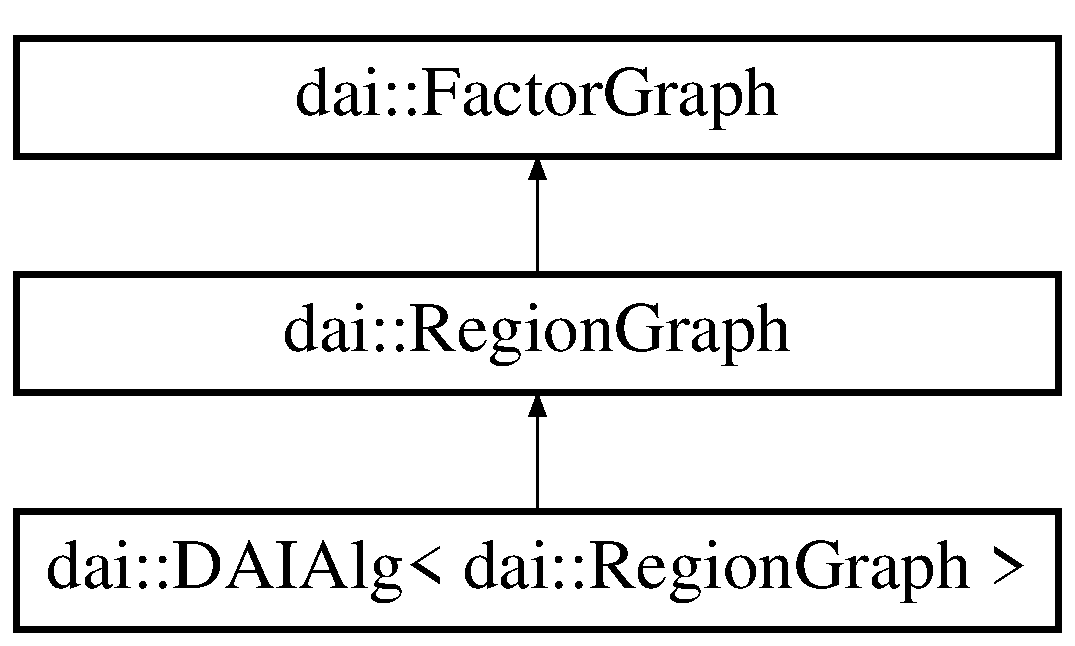
\includegraphics[height=3cm]{classdai_1_1RegionGraph}
\end{center}
\end{figure}


\subsection{Detailed Description}
A \hyperlink{classdai_1_1RegionGraph}{RegionGraph} is a bipartite graph consisting of outer regions (type \hyperlink{classdai_1_1FRegion}{FRegion}) and inner regions (type \hyperlink{classdai_1_1Region}{Region}). \subsection*{Public Types}
\begin{CompactItemize}
\item 
\hypertarget{classdai_1_1FactorGraph_1552870151bb7f7a88b3120a777c1056}{
typedef \hyperlink{structdai_1_1BipartiteGraph_1_1Neighbor}{BipartiteGraph::Neighbor} \hyperlink{classdai_1_1FactorGraph_1552870151bb7f7a88b3120a777c1056}{Neighbor}}
\label{classdai_1_1FactorGraph_1552870151bb7f7a88b3120a777c1056}

\begin{CompactList}\small\item\em Shorthand for \hyperlink{structdai_1_1BipartiteGraph_1_1Neighbor}{BipartiteGraph::Neighbor}. \item\end{CompactList}\item 
\hypertarget{classdai_1_1FactorGraph_326942db90fe2dbdf99041d5d966019e}{
typedef \hyperlink{classdai_1_1BipartiteGraph_031237b607d2868b80052e71b4149b29}{BipartiteGraph::Neighbors} \hyperlink{classdai_1_1FactorGraph_326942db90fe2dbdf99041d5d966019e}{Neighbors}}
\label{classdai_1_1FactorGraph_326942db90fe2dbdf99041d5d966019e}

\begin{CompactList}\small\item\em Shorthand for \hyperlink{classdai_1_1BipartiteGraph_031237b607d2868b80052e71b4149b29}{BipartiteGraph::Neighbors}. \item\end{CompactList}\item 
\hypertarget{classdai_1_1FactorGraph_743243688f787418eff5352140980119}{
typedef \hyperlink{classdai_1_1BipartiteGraph_ff511d0eba0fd2956c08b602029ba95f}{BipartiteGraph::Edge} \hyperlink{classdai_1_1FactorGraph_743243688f787418eff5352140980119}{Edge}}
\label{classdai_1_1FactorGraph_743243688f787418eff5352140980119}

\begin{CompactList}\small\item\em Shorthand for \hyperlink{classdai_1_1BipartiteGraph_ff511d0eba0fd2956c08b602029ba95f}{BipartiteGraph::Edge}. \item\end{CompactList}\end{CompactItemize}
\subsection*{Public Member Functions}
\begin{CompactItemize}
\item 
\hypertarget{classdai_1_1RegionGraph_3d60a9dbf05e5b203ccbe021d8d3b080}{
\hyperlink{classdai_1_1RegionGraph_3d60a9dbf05e5b203ccbe021d8d3b080}{RegionGraph} ()}
\label{classdai_1_1RegionGraph_3d60a9dbf05e5b203ccbe021d8d3b080}

\begin{CompactList}\small\item\em Default constructor. \item\end{CompactList}\item 
\hypertarget{classdai_1_1RegionGraph_ebc7b75de029b1915d1b86e3a769bb9f}{
\hyperlink{classdai_1_1RegionGraph_ebc7b75de029b1915d1b86e3a769bb9f}{RegionGraph} (const \hyperlink{classdai_1_1FactorGraph}{FactorGraph} \&fg)}
\label{classdai_1_1RegionGraph_ebc7b75de029b1915d1b86e3a769bb9f}

\begin{CompactList}\small\item\em Constructs a \hyperlink{classdai_1_1RegionGraph}{RegionGraph} from a \hyperlink{classdai_1_1FactorGraph}{FactorGraph}. \item\end{CompactList}\item 
\hypertarget{classdai_1_1RegionGraph_e5c5becfae3721397e6958e05499e1e5}{
\hyperlink{classdai_1_1RegionGraph_e5c5becfae3721397e6958e05499e1e5}{RegionGraph} (const \hyperlink{classdai_1_1FactorGraph}{FactorGraph} \&fg, const std::vector$<$ \hyperlink{classdai_1_1Region}{Region} $>$ \&ors, const std::vector$<$ \hyperlink{classdai_1_1Region}{Region} $>$ \&irs, const std::vector$<$ std::pair$<$ size\_\-t, size\_\-t $>$ $>$ \&edges)}
\label{classdai_1_1RegionGraph_e5c5becfae3721397e6958e05499e1e5}

\begin{CompactList}\small\item\em Constructs a \hyperlink{classdai_1_1RegionGraph}{RegionGraph} from a \hyperlink{classdai_1_1FactorGraph}{FactorGraph}, a vector of outer regions, a vector of inner regions and a vector of edges. \item\end{CompactList}\item 
\hypertarget{classdai_1_1RegionGraph_bbb85bc05de8136b5ff12ba66df7867b}{
\hyperlink{classdai_1_1RegionGraph_bbb85bc05de8136b5ff12ba66df7867b}{RegionGraph} (const \hyperlink{classdai_1_1FactorGraph}{FactorGraph} \&fg, const std::vector$<$ \hyperlink{classdai_1_1VarSet}{VarSet} $>$ \&cl)}
\label{classdai_1_1RegionGraph_bbb85bc05de8136b5ff12ba66df7867b}

\begin{CompactList}\small\item\em Constructs a \hyperlink{classdai_1_1RegionGraph}{RegionGraph} from a \hyperlink{classdai_1_1FactorGraph}{FactorGraph} and a vector of outer VarSets (CVM style). \item\end{CompactList}\item 
\hypertarget{classdai_1_1RegionGraph_cfd5a9c99ed3725a4630b7900a4a32e1}{
\hyperlink{classdai_1_1RegionGraph_cfd5a9c99ed3725a4630b7900a4a32e1}{RegionGraph} (const \hyperlink{classdai_1_1RegionGraph}{RegionGraph} \&x)}
\label{classdai_1_1RegionGraph_cfd5a9c99ed3725a4630b7900a4a32e1}

\begin{CompactList}\small\item\em Copy constructor. \item\end{CompactList}\item 
\hypertarget{classdai_1_1RegionGraph_deb3664382c754e79148267239894ab3}{
\hyperlink{classdai_1_1RegionGraph}{RegionGraph} \& \hyperlink{classdai_1_1RegionGraph_deb3664382c754e79148267239894ab3}{operator=} (const \hyperlink{classdai_1_1RegionGraph}{RegionGraph} \&x)}
\label{classdai_1_1RegionGraph_deb3664382c754e79148267239894ab3}

\begin{CompactList}\small\item\em Assignment operator. \item\end{CompactList}\item 
\hypertarget{classdai_1_1RegionGraph_2d67c462b308b3acbec965ba10f1e6e2}{
virtual \hyperlink{classdai_1_1RegionGraph}{RegionGraph} $\ast$ \hyperlink{classdai_1_1RegionGraph_2d67c462b308b3acbec965ba10f1e6e2}{clone} () const }
\label{classdai_1_1RegionGraph_2d67c462b308b3acbec965ba10f1e6e2}

\begin{CompactList}\small\item\em Clone $\ast$this (virtual copy constructor). \item\end{CompactList}\item 
\hypertarget{classdai_1_1RegionGraph_1d68790861f6eb1f6e50ddb75c6c3201}{
virtual \hyperlink{classdai_1_1RegionGraph}{RegionGraph} $\ast$ \hyperlink{classdai_1_1RegionGraph_1d68790861f6eb1f6e50ddb75c6c3201}{create} () const }
\label{classdai_1_1RegionGraph_1d68790861f6eb1f6e50ddb75c6c3201}

\begin{CompactList}\small\item\em Create (virtual default constructor). \item\end{CompactList}\item 
\hypertarget{classdai_1_1RegionGraph_3ff68e22e5bbd6a37142f6d759956fdf}{
virtual void \hyperlink{classdai_1_1RegionGraph_3ff68e22e5bbd6a37142f6d759956fdf}{setFactor} (size\_\-t I, const \hyperlink{classdai_1_1TFactor}{Factor} \&newFactor, bool backup=false)}
\label{classdai_1_1RegionGraph_3ff68e22e5bbd6a37142f6d759956fdf}

\begin{CompactList}\small\item\em Set the content of the I'th factor and make a backup of its old content if backup == true. \item\end{CompactList}\item 
\hypertarget{classdai_1_1RegionGraph_d856e0dce255c429a4cddaba99c7d0f0}{
virtual void \hyperlink{classdai_1_1RegionGraph_d856e0dce255c429a4cddaba99c7d0f0}{setFactors} (const std::map$<$ size\_\-t, \hyperlink{classdai_1_1TFactor}{Factor} $>$ \&facs, bool backup=false)}
\label{classdai_1_1RegionGraph_d856e0dce255c429a4cddaba99c7d0f0}

\begin{CompactList}\small\item\em Set the contents of all factors as specified by facs and make a backup of the old contents if backup == true. \item\end{CompactList}\item 
\hypertarget{classdai_1_1RegionGraph_d32f10da72fca83bc4fd7c60bf771a40}{
const \hyperlink{classdai_1_1FRegion}{FRegion} \& \hyperlink{classdai_1_1RegionGraph_d32f10da72fca83bc4fd7c60bf771a40}{OR} (size\_\-t alpha) const }
\label{classdai_1_1RegionGraph_d32f10da72fca83bc4fd7c60bf771a40}

\begin{CompactList}\small\item\em Provides read access to outer region. \item\end{CompactList}\item 
\hypertarget{classdai_1_1RegionGraph_70aca393e89fdb7e4dc7535e9bf95676}{
\hyperlink{classdai_1_1FRegion}{FRegion} \& \hyperlink{classdai_1_1RegionGraph_70aca393e89fdb7e4dc7535e9bf95676}{OR} (size\_\-t alpha)}
\label{classdai_1_1RegionGraph_70aca393e89fdb7e4dc7535e9bf95676}

\begin{CompactList}\small\item\em Provides access to outer region. \item\end{CompactList}\item 
\hypertarget{classdai_1_1RegionGraph_fc3b5514a3667829d984e1b9bdf8f3b6}{
const \hyperlink{classdai_1_1Region}{Region} \& \hyperlink{classdai_1_1RegionGraph_fc3b5514a3667829d984e1b9bdf8f3b6}{IR} (size\_\-t beta) const }
\label{classdai_1_1RegionGraph_fc3b5514a3667829d984e1b9bdf8f3b6}

\begin{CompactList}\small\item\em Provides read access to inner region. \item\end{CompactList}\item 
\hypertarget{classdai_1_1RegionGraph_8cad2cb98698539d459ba2d0dbd5a14f}{
\hyperlink{classdai_1_1Region}{Region} \& \hyperlink{classdai_1_1RegionGraph_8cad2cb98698539d459ba2d0dbd5a14f}{IR} (size\_\-t beta)}
\label{classdai_1_1RegionGraph_8cad2cb98698539d459ba2d0dbd5a14f}

\begin{CompactList}\small\item\em Provides access to inner region. \item\end{CompactList}\item 
\hypertarget{classdai_1_1RegionGraph_383bfd8e082054b87170ad6f9bf13cc3}{
size\_\-t \hyperlink{classdai_1_1RegionGraph_383bfd8e082054b87170ad6f9bf13cc3}{nrORs} () const }
\label{classdai_1_1RegionGraph_383bfd8e082054b87170ad6f9bf13cc3}

\begin{CompactList}\small\item\em Returns number of outer regions. \item\end{CompactList}\item 
\hypertarget{classdai_1_1RegionGraph_b8038c7a58f3b50c0e8b0229522f20b7}{
size\_\-t \hyperlink{classdai_1_1RegionGraph_b8038c7a58f3b50c0e8b0229522f20b7}{nrIRs} () const }
\label{classdai_1_1RegionGraph_b8038c7a58f3b50c0e8b0229522f20b7}

\begin{CompactList}\small\item\em Returns number of inner regions. \item\end{CompactList}\item 
\hypertarget{classdai_1_1RegionGraph_a5e0c7aa216c1589b12c985f4c1712eb}{
const \hyperlink{classdai_1_1FactorGraph_326942db90fe2dbdf99041d5d966019e}{Neighbors} \& \hyperlink{classdai_1_1RegionGraph_a5e0c7aa216c1589b12c985f4c1712eb}{nbOR} (size\_\-t alpha) const }
\label{classdai_1_1RegionGraph_a5e0c7aa216c1589b12c985f4c1712eb}

\begin{CompactList}\small\item\em Provides read access to neighbors of outer region. \item\end{CompactList}\item 
\hypertarget{classdai_1_1RegionGraph_90cb59fcc10f82fa7f97b145c34df598}{
\hyperlink{classdai_1_1FactorGraph_326942db90fe2dbdf99041d5d966019e}{Neighbors} \& \hyperlink{classdai_1_1RegionGraph_90cb59fcc10f82fa7f97b145c34df598}{nbOR} (size\_\-t alpha)}
\label{classdai_1_1RegionGraph_90cb59fcc10f82fa7f97b145c34df598}

\begin{CompactList}\small\item\em Provides full access to neighbors of outer region. \item\end{CompactList}\item 
\hypertarget{classdai_1_1RegionGraph_aee9b80df34d423ce0ad9e9465e1932b}{
const \hyperlink{classdai_1_1FactorGraph_326942db90fe2dbdf99041d5d966019e}{Neighbors} \& \hyperlink{classdai_1_1RegionGraph_aee9b80df34d423ce0ad9e9465e1932b}{nbIR} (size\_\-t beta) const }
\label{classdai_1_1RegionGraph_aee9b80df34d423ce0ad9e9465e1932b}

\begin{CompactList}\small\item\em Provides read access to neighbors of inner region. \item\end{CompactList}\item 
\hypertarget{classdai_1_1RegionGraph_f4051be69169e92fe652e6024389324b}{
\hyperlink{classdai_1_1FactorGraph_326942db90fe2dbdf99041d5d966019e}{Neighbors} \& \hyperlink{classdai_1_1RegionGraph_f4051be69169e92fe652e6024389324b}{nbIR} (size\_\-t beta)}
\label{classdai_1_1RegionGraph_f4051be69169e92fe652e6024389324b}

\begin{CompactList}\small\item\em Provides full access to neighbors of inner region. \item\end{CompactList}\item 
\hypertarget{classdai_1_1RegionGraph_014b5c5df33b4b47b68e4caf7485f1aa}{
void \hyperlink{classdai_1_1RegionGraph_014b5c5df33b4b47b68e4caf7485f1aa}{Calc\_\-Counting\_\-Numbers} ()}
\label{classdai_1_1RegionGraph_014b5c5df33b4b47b68e4caf7485f1aa}

\begin{CompactList}\small\item\em Calculates counting numbers of inner regions based upon counting numbers of outer regions. \item\end{CompactList}\item 
\hypertarget{classdai_1_1RegionGraph_16b1c05909e5bb52c472fd15e9791f90}{
bool \hyperlink{classdai_1_1RegionGraph_16b1c05909e5bb52c472fd15e9791f90}{Check\_\-Counting\_\-Numbers} ()}
\label{classdai_1_1RegionGraph_16b1c05909e5bb52c472fd15e9791f90}

\begin{CompactList}\small\item\em Check whether the counting numbers are valid. \item\end{CompactList}\item 
\hypertarget{classdai_1_1RegionGraph_642af0274d25e08fa4c2ec92314477ee}{
void \hyperlink{classdai_1_1RegionGraph_642af0274d25e08fa4c2ec92314477ee}{RecomputeORs} ()}
\label{classdai_1_1RegionGraph_642af0274d25e08fa4c2ec92314477ee}

\begin{CompactList}\small\item\em Recompute all outer regions. \item\end{CompactList}\item 
\hypertarget{classdai_1_1RegionGraph_5e867cca791a16e5538b175eb0193b97}{
void \hyperlink{classdai_1_1RegionGraph_5e867cca791a16e5538b175eb0193b97}{RecomputeORs} (const \hyperlink{classdai_1_1VarSet}{VarSet} \&ns)}
\label{classdai_1_1RegionGraph_5e867cca791a16e5538b175eb0193b97}

\begin{CompactList}\small\item\em Recompute all outer regions involving the variables in ns. \item\end{CompactList}\item 
\hypertarget{classdai_1_1RegionGraph_04b34775be9a380334f16c61505e9e54}{
void \hyperlink{classdai_1_1RegionGraph_04b34775be9a380334f16c61505e9e54}{RecomputeOR} (size\_\-t I)}
\label{classdai_1_1RegionGraph_04b34775be9a380334f16c61505e9e54}

\begin{CompactList}\small\item\em Recompute all outer regions involving factor I. \item\end{CompactList}\item 
\hypertarget{classdai_1_1FactorGraph_87036afc568a8658dee9bff52f8fd3e1}{
const \hyperlink{classdai_1_1Var}{Var} \& \hyperlink{classdai_1_1FactorGraph_87036afc568a8658dee9bff52f8fd3e1}{var} (size\_\-t i) const }
\label{classdai_1_1FactorGraph_87036afc568a8658dee9bff52f8fd3e1}

\begin{CompactList}\small\item\em Returns const reference to i'th variable. \item\end{CompactList}\item 
\hypertarget{classdai_1_1FactorGraph_4e82ddbe1e2ca8a58bc7aec4d9fa61b6}{
const std::vector$<$ \hyperlink{classdai_1_1Var}{Var} $>$ \& \hyperlink{classdai_1_1FactorGraph_4e82ddbe1e2ca8a58bc7aec4d9fa61b6}{vars} () const }
\label{classdai_1_1FactorGraph_4e82ddbe1e2ca8a58bc7aec4d9fa61b6}

\begin{CompactList}\small\item\em Returns const reference to all factors. \item\end{CompactList}\item 
\hypertarget{classdai_1_1FactorGraph_4f73bace8b2ecd16654116467f38045b}{
\hyperlink{classdai_1_1TFactor}{Factor} \& \hyperlink{classdai_1_1FactorGraph_4f73bace8b2ecd16654116467f38045b}{factor} (size\_\-t I)}
\label{classdai_1_1FactorGraph_4f73bace8b2ecd16654116467f38045b}

\begin{CompactList}\small\item\em Returns reference to I'th factor. \item\end{CompactList}\item 
\hypertarget{classdai_1_1FactorGraph_9a930964b0d006bb0d6ace88fb1da481}{
const \hyperlink{classdai_1_1TFactor}{Factor} \& \hyperlink{classdai_1_1FactorGraph_9a930964b0d006bb0d6ace88fb1da481}{factor} (size\_\-t I) const }
\label{classdai_1_1FactorGraph_9a930964b0d006bb0d6ace88fb1da481}

\begin{CompactList}\small\item\em Returns const reference to I'th factor. \item\end{CompactList}\item 
\hypertarget{classdai_1_1FactorGraph_35030e580fdcab5abd877f0e0bd883d5}{
const std::vector$<$ \hyperlink{classdai_1_1TFactor}{Factor} $>$ \& \hyperlink{classdai_1_1FactorGraph_35030e580fdcab5abd877f0e0bd883d5}{factors} () const }
\label{classdai_1_1FactorGraph_35030e580fdcab5abd877f0e0bd883d5}

\begin{CompactList}\small\item\em Returns const reference to all factors. \item\end{CompactList}\item 
\hypertarget{classdai_1_1FactorGraph_107d707b4ef22d83f19c40989c227d5d}{
size\_\-t \hyperlink{classdai_1_1FactorGraph_107d707b4ef22d83f19c40989c227d5d}{nrVars} () const }
\label{classdai_1_1FactorGraph_107d707b4ef22d83f19c40989c227d5d}

\begin{CompactList}\small\item\em Returns number of variables. \item\end{CompactList}\item 
\hypertarget{classdai_1_1FactorGraph_de52f40e90ae438c985f9568811654a9}{
size\_\-t \hyperlink{classdai_1_1FactorGraph_de52f40e90ae438c985f9568811654a9}{nrFactors} () const }
\label{classdai_1_1FactorGraph_de52f40e90ae438c985f9568811654a9}

\begin{CompactList}\small\item\em Returns number of factors. \item\end{CompactList}\item 
\hypertarget{classdai_1_1FactorGraph_a1b94e2729ef0a941f6dbee1b7ea1b24}{
size\_\-t \hyperlink{classdai_1_1FactorGraph_a1b94e2729ef0a941f6dbee1b7ea1b24}{nrEdges} () const }
\label{classdai_1_1FactorGraph_a1b94e2729ef0a941f6dbee1b7ea1b24}

\begin{CompactList}\small\item\em Calculates number of edges. \item\end{CompactList}\item 
\hypertarget{classdai_1_1FactorGraph_dce52503905082b5288da10147358d03}{
const \hyperlink{classdai_1_1FactorGraph_326942db90fe2dbdf99041d5d966019e}{Neighbors} \& \hyperlink{classdai_1_1FactorGraph_dce52503905082b5288da10147358d03}{nbV} (size\_\-t i) const }
\label{classdai_1_1FactorGraph_dce52503905082b5288da10147358d03}

\begin{CompactList}\small\item\em Provides read access to neighbors of variable. \item\end{CompactList}\item 
\hypertarget{classdai_1_1FactorGraph_1b69b08da98de54b911cb8c1245d3622}{
\hyperlink{classdai_1_1FactorGraph_326942db90fe2dbdf99041d5d966019e}{Neighbors} \& \hyperlink{classdai_1_1FactorGraph_1b69b08da98de54b911cb8c1245d3622}{nbV} (size\_\-t i)}
\label{classdai_1_1FactorGraph_1b69b08da98de54b911cb8c1245d3622}

\begin{CompactList}\small\item\em Provides full access to neighbors of variable. \item\end{CompactList}\item 
\hypertarget{classdai_1_1FactorGraph_cffe2211b3a588c92cdabe40071f0c77}{
const \hyperlink{structdai_1_1BipartiteGraph_1_1Neighbor}{Neighbor} \& \hyperlink{classdai_1_1FactorGraph_cffe2211b3a588c92cdabe40071f0c77}{nbV} (size\_\-t i, size\_\-t \_\-I) const }
\label{classdai_1_1FactorGraph_cffe2211b3a588c92cdabe40071f0c77}

\begin{CompactList}\small\item\em Provides read access to neighbor of variable. \item\end{CompactList}\item 
\hypertarget{classdai_1_1FactorGraph_06ee72e5307fb2aa1af3cfcfec1fc449}{
\hyperlink{structdai_1_1BipartiteGraph_1_1Neighbor}{Neighbor} \& \hyperlink{classdai_1_1FactorGraph_06ee72e5307fb2aa1af3cfcfec1fc449}{nbV} (size\_\-t i, size\_\-t \_\-I)}
\label{classdai_1_1FactorGraph_06ee72e5307fb2aa1af3cfcfec1fc449}

\begin{CompactList}\small\item\em Provides full access to neighbor of variable. \item\end{CompactList}\item 
\hypertarget{classdai_1_1FactorGraph_d3ae273e55d134fe0eb6ed67492953d7}{
const \hyperlink{classdai_1_1FactorGraph_326942db90fe2dbdf99041d5d966019e}{Neighbors} \& \hyperlink{classdai_1_1FactorGraph_d3ae273e55d134fe0eb6ed67492953d7}{nbF} (size\_\-t I) const }
\label{classdai_1_1FactorGraph_d3ae273e55d134fe0eb6ed67492953d7}

\begin{CompactList}\small\item\em Provides read access to neighbors of factor. \item\end{CompactList}\item 
\hypertarget{classdai_1_1FactorGraph_10914ba06b0c939cc5d1f3fe7a1c27c2}{
\hyperlink{classdai_1_1FactorGraph_326942db90fe2dbdf99041d5d966019e}{Neighbors} \& \hyperlink{classdai_1_1FactorGraph_10914ba06b0c939cc5d1f3fe7a1c27c2}{nbF} (size\_\-t I)}
\label{classdai_1_1FactorGraph_10914ba06b0c939cc5d1f3fe7a1c27c2}

\begin{CompactList}\small\item\em Provides full access to neighbors of factor. \item\end{CompactList}\item 
\hypertarget{classdai_1_1FactorGraph_882dbd45fd323d8020df45c0d23a85da}{
const \hyperlink{structdai_1_1BipartiteGraph_1_1Neighbor}{Neighbor} \& \hyperlink{classdai_1_1FactorGraph_882dbd45fd323d8020df45c0d23a85da}{nbF} (size\_\-t I, size\_\-t \_\-i) const }
\label{classdai_1_1FactorGraph_882dbd45fd323d8020df45c0d23a85da}

\begin{CompactList}\small\item\em Provides read access to neighbor of factor. \item\end{CompactList}\item 
\hypertarget{classdai_1_1FactorGraph_bb04181cfad3d5e461bff89c6fa0f83a}{
\hyperlink{structdai_1_1BipartiteGraph_1_1Neighbor}{Neighbor} \& \hyperlink{classdai_1_1FactorGraph_bb04181cfad3d5e461bff89c6fa0f83a}{nbF} (size\_\-t I, size\_\-t \_\-i)}
\label{classdai_1_1FactorGraph_bb04181cfad3d5e461bff89c6fa0f83a}

\begin{CompactList}\small\item\em Provides full access to neighbor of factor. \item\end{CompactList}\item 
\hypertarget{classdai_1_1FactorGraph_25f3ffef7d09bbea7fe4ec69840395b3}{
size\_\-t \hyperlink{classdai_1_1FactorGraph_25f3ffef7d09bbea7fe4ec69840395b3}{findVar} (const \hyperlink{classdai_1_1Var}{Var} \&n) const }
\label{classdai_1_1FactorGraph_25f3ffef7d09bbea7fe4ec69840395b3}

\begin{CompactList}\small\item\em Returns the index of a particular variable. \item\end{CompactList}\item 
\hypertarget{classdai_1_1FactorGraph_ae887d817c2e6e081d91e54083abc6ad}{
std::set$<$ size\_\-t $>$ \hyperlink{classdai_1_1FactorGraph_ae887d817c2e6e081d91e54083abc6ad}{findVars} (\hyperlink{classdai_1_1VarSet}{VarSet} \&ns) const }
\label{classdai_1_1FactorGraph_ae887d817c2e6e081d91e54083abc6ad}

\begin{CompactList}\small\item\em Returns a set of indexes corresponding to a set of variables. \item\end{CompactList}\item 
\hypertarget{classdai_1_1FactorGraph_c7a2074bd52b7cb35a6473208140bb34}{
size\_\-t \hyperlink{classdai_1_1FactorGraph_c7a2074bd52b7cb35a6473208140bb34}{findFactor} (const \hyperlink{classdai_1_1VarSet}{VarSet} \&ns) const }
\label{classdai_1_1FactorGraph_c7a2074bd52b7cb35a6473208140bb34}

\begin{CompactList}\small\item\em Returns index of the first factor that depends on the variables. \item\end{CompactList}\item 
\hypertarget{classdai_1_1FactorGraph_b0c02cc79dbbe2d23f67281b7af76ed1}{
\hyperlink{classdai_1_1VarSet}{VarSet} \hyperlink{classdai_1_1FactorGraph_b0c02cc79dbbe2d23f67281b7af76ed1}{Delta} (unsigned i) const }
\label{classdai_1_1FactorGraph_b0c02cc79dbbe2d23f67281b7af76ed1}

\begin{CompactList}\small\item\em Return all variables that occur in a factor involving the i'th variable, itself included. \item\end{CompactList}\item 
\hypertarget{classdai_1_1FactorGraph_6c74472eacbfc029cc6cc5ba4e865b1d}{
\hyperlink{classdai_1_1VarSet}{VarSet} \hyperlink{classdai_1_1FactorGraph_6c74472eacbfc029cc6cc5ba4e865b1d}{Delta} (const \hyperlink{classdai_1_1VarSet}{VarSet} \&ns) const }
\label{classdai_1_1FactorGraph_6c74472eacbfc029cc6cc5ba4e865b1d}

\begin{CompactList}\small\item\em Return all variables that occur in a factor involving some variable in ns, ns itself included. \item\end{CompactList}\item 
\hypertarget{classdai_1_1FactorGraph_bd749cf993fdc774b993e72d7d07bc40}{
\hyperlink{classdai_1_1VarSet}{VarSet} \hyperlink{classdai_1_1FactorGraph_bd749cf993fdc774b993e72d7d07bc40}{delta} (unsigned i) const }
\label{classdai_1_1FactorGraph_bd749cf993fdc774b993e72d7d07bc40}

\begin{CompactList}\small\item\em Return all variables that occur in a factor involving the i'th variable, n itself excluded. \item\end{CompactList}\item 
\hypertarget{classdai_1_1FactorGraph_358d94bc2adb7be856ea7b60e2e21096}{
\hyperlink{classdai_1_1VarSet}{VarSet} \hyperlink{classdai_1_1FactorGraph_358d94bc2adb7be856ea7b60e2e21096}{delta} (const \hyperlink{classdai_1_1VarSet}{VarSet} \&ns) const }
\label{classdai_1_1FactorGraph_358d94bc2adb7be856ea7b60e2e21096}

\begin{CompactList}\small\item\em Return all variables that occur in a factor involving some variable in ns, ns itself excluded. \item\end{CompactList}\item 
virtual void \hyperlink{classdai_1_1FactorGraph_3cb7d91ca96090372bd0aacbf70a8948}{clamp} (const \hyperlink{classdai_1_1Var}{Var} \&n, size\_\-t i, bool backup=false)
\item 
\hypertarget{classdai_1_1FactorGraph_42791a748401710f846e3ac1a3d7a10a}{
virtual void \hyperlink{classdai_1_1FactorGraph_42791a748401710f846e3ac1a3d7a10a}{makeCavity} (unsigned i, bool backup=false)}
\label{classdai_1_1FactorGraph_42791a748401710f846e3ac1a3d7a10a}

\begin{CompactList}\small\item\em Set all factors interacting with the i'th variable 1. \item\end{CompactList}\item 
\hypertarget{classdai_1_1FactorGraph_6965352b4e04b47fd7ad551d9c1916f2}{
virtual void \hyperlink{classdai_1_1FactorGraph_6965352b4e04b47fd7ad551d9c1916f2}{backupFactors} (const std::set$<$ size\_\-t $>$ \&facs)}
\label{classdai_1_1FactorGraph_6965352b4e04b47fd7ad551d9c1916f2}

\begin{CompactList}\small\item\em Backup the factors specified by indices in facs. \item\end{CompactList}\item 
\hypertarget{classdai_1_1FactorGraph_8b3606b4ee589e4a0fb8fcdbdff97bae}{
void \hyperlink{classdai_1_1FactorGraph_8b3606b4ee589e4a0fb8fcdbdff97bae}{backupFactors} (const \hyperlink{classdai_1_1VarSet}{VarSet} \&ns)}
\label{classdai_1_1FactorGraph_8b3606b4ee589e4a0fb8fcdbdff97bae}

\begin{CompactList}\small\item\em Makes a backup of all factors connected to a set of variables. \item\end{CompactList}\item 
\hypertarget{classdai_1_1FactorGraph_0fe64720797972b14f1b41486d339f81}{
virtual void \hyperlink{classdai_1_1FactorGraph_0fe64720797972b14f1b41486d339f81}{restoreFactors} ()}
\label{classdai_1_1FactorGraph_0fe64720797972b14f1b41486d339f81}

\begin{CompactList}\small\item\em Restore all factors to the backup copies. \item\end{CompactList}\item 
\hypertarget{classdai_1_1FactorGraph_4e042494d8e453005d0c8bfd788dc687}{
void \hyperlink{classdai_1_1FactorGraph_4e042494d8e453005d0c8bfd788dc687}{restoreFactors} (const \hyperlink{classdai_1_1VarSet}{VarSet} \&ns)}
\label{classdai_1_1FactorGraph_4e042494d8e453005d0c8bfd788dc687}

\begin{CompactList}\small\item\em Restores all factors connected to a set of variables from their backups. \item\end{CompactList}\item 
\hypertarget{classdai_1_1FactorGraph_d1e3c45492a64959fec4736adf555528}{
bool \hyperlink{classdai_1_1FactorGraph_d1e3c45492a64959fec4736adf555528}{isConnected} () const }
\label{classdai_1_1FactorGraph_d1e3c45492a64959fec4736adf555528}

\begin{CompactList}\small\item\em Returns true if the \hyperlink{classdai_1_1FactorGraph}{FactorGraph} is connected. \item\end{CompactList}\item 
\hypertarget{classdai_1_1FactorGraph_a4e258a9fc003b49491529dfcf45d56a}{
bool \hyperlink{classdai_1_1FactorGraph_a4e258a9fc003b49491529dfcf45d56a}{isTree} () const }
\label{classdai_1_1FactorGraph_a4e258a9fc003b49491529dfcf45d56a}

\begin{CompactList}\small\item\em Returns true if the \hyperlink{classdai_1_1FactorGraph}{FactorGraph} is a tree. \item\end{CompactList}\item 
\hypertarget{classdai_1_1FactorGraph_f1b9c45ee2670aca3d04c2733193f611}{
bool \hyperlink{classdai_1_1FactorGraph_f1b9c45ee2670aca3d04c2733193f611}{isPairwise} () const }
\label{classdai_1_1FactorGraph_f1b9c45ee2670aca3d04c2733193f611}

\begin{CompactList}\small\item\em Returns true if each factor depends on at most two variables. \item\end{CompactList}\item 
\hypertarget{classdai_1_1FactorGraph_f3c0f08798db25845cb518ec6cccbd05}{
bool \hyperlink{classdai_1_1FactorGraph_f3c0f08798db25845cb518ec6cccbd05}{isBinary} () const }
\label{classdai_1_1FactorGraph_f3c0f08798db25845cb518ec6cccbd05}

\begin{CompactList}\small\item\em Returns true if each variable has only two possible values. \item\end{CompactList}\item 
\hypertarget{classdai_1_1FactorGraph_89ee98ae7d3bc1723452e1c11ace4b51}{
void \hyperlink{classdai_1_1FactorGraph_89ee98ae7d3bc1723452e1c11ace4b51}{ReadFromFile} (const char $\ast$filename)}
\label{classdai_1_1FactorGraph_89ee98ae7d3bc1723452e1c11ace4b51}

\begin{CompactList}\small\item\em Reads a \hyperlink{classdai_1_1FactorGraph}{FactorGraph} from a file. \item\end{CompactList}\item 
\hypertarget{classdai_1_1FactorGraph_0916dbc2ac40ad7e5bf0cca9740d3c2c}{
void \hyperlink{classdai_1_1FactorGraph_0916dbc2ac40ad7e5bf0cca9740d3c2c}{WriteToFile} (const char $\ast$filename) const }
\label{classdai_1_1FactorGraph_0916dbc2ac40ad7e5bf0cca9740d3c2c}

\begin{CompactList}\small\item\em Writes a \hyperlink{classdai_1_1FactorGraph}{FactorGraph} to a file. \item\end{CompactList}\item 
\hypertarget{classdai_1_1FactorGraph_607c9a821e789121cf2ccbfacc5f8d5f}{
void \hyperlink{classdai_1_1FactorGraph_607c9a821e789121cf2ccbfacc5f8d5f}{printDot} (std::ostream \&os) const }
\label{classdai_1_1FactorGraph_607c9a821e789121cf2ccbfacc5f8d5f}

\begin{CompactList}\small\item\em Writes a \hyperlink{classdai_1_1FactorGraph}{FactorGraph} to a GraphViz .dot file. \item\end{CompactList}\item 
\hypertarget{classdai_1_1FactorGraph_9cd8cc192cac877725b2bae9f3e61a9f}{
std::vector$<$ \hyperlink{classdai_1_1VarSet}{VarSet} $>$ \hyperlink{classdai_1_1FactorGraph_9cd8cc192cac877725b2bae9f3e61a9f}{Cliques} () const }
\label{classdai_1_1FactorGraph_9cd8cc192cac877725b2bae9f3e61a9f}

\begin{CompactList}\small\item\em Returns the cliques in this \hyperlink{classdai_1_1FactorGraph}{FactorGraph}. \item\end{CompactList}\item 
\hyperlink{classdai_1_1FactorGraph}{FactorGraph} \hyperlink{classdai_1_1FactorGraph_915d21c0da8c2c1f342371bef6adb0f5}{clamped} (const \hyperlink{classdai_1_1Var}{Var} \&v\_\-i, size\_\-t x) const 
\begin{CompactList}\small\item\em Clamp variable v\_\-i to value state (i.e. multiply with a Kronecker delta $\delta_{x_{v_i},x}$);. \item\end{CompactList}\item 
\hypertarget{classdai_1_1FactorGraph_213527d7bcd00ccedce6276311332500}{
\hyperlink{classdai_1_1FactorGraph}{FactorGraph} \hyperlink{classdai_1_1FactorGraph_213527d7bcd00ccedce6276311332500}{maximalFactors} () const }
\label{classdai_1_1FactorGraph_213527d7bcd00ccedce6276311332500}

\begin{CompactList}\small\item\em Returns a copy of $\ast$this, where all factors that are subsumed by some larger factor are merged with the larger factors. \item\end{CompactList}\item 
\hypertarget{classdai_1_1FactorGraph_39ce217df7d9ea85b2b04b8d65101230}{
void \hyperlink{classdai_1_1FactorGraph_39ce217df7d9ea85b2b04b8d65101230}{restoreFactor} (size\_\-t I)}
\label{classdai_1_1FactorGraph_39ce217df7d9ea85b2b04b8d65101230}

\begin{CompactList}\small\item\em Makes a backup of the I'th Factor. \item\end{CompactList}\item 
\hypertarget{classdai_1_1FactorGraph_e2fe32e831db3e649e6ddd66762fea7c}{
void \hyperlink{classdai_1_1FactorGraph_e2fe32e831db3e649e6ddd66762fea7c}{backupFactor} (size\_\-t I)}
\label{classdai_1_1FactorGraph_e2fe32e831db3e649e6ddd66762fea7c}

\begin{CompactList}\small\item\em Restores the I'th Factor from the backup (it should be backed up first). \item\end{CompactList}\end{CompactItemize}
\subsection*{Public Attributes}
\begin{CompactItemize}
\item 
\hypertarget{classdai_1_1RegionGraph_baca33a49ccbcb787c3d459398b47047}{
\hyperlink{classdai_1_1BipartiteGraph}{BipartiteGraph} \hyperlink{classdai_1_1RegionGraph_baca33a49ccbcb787c3d459398b47047}{G}}
\label{classdai_1_1RegionGraph_baca33a49ccbcb787c3d459398b47047}

\begin{CompactList}\small\item\em Stores the neighborhood structure. \item\end{CompactList}\item 
\hypertarget{classdai_1_1RegionGraph_5c94c84a601c9b29cfe75da8562dfed8}{
std::vector$<$ \hyperlink{classdai_1_1FRegion}{FRegion} $>$ \hyperlink{classdai_1_1RegionGraph_5c94c84a601c9b29cfe75da8562dfed8}{ORs}}
\label{classdai_1_1RegionGraph_5c94c84a601c9b29cfe75da8562dfed8}

\begin{CompactList}\small\item\em The outer regions (corresponding to nodes of type 1). \item\end{CompactList}\item 
\hypertarget{classdai_1_1RegionGraph_e3c3173e62a9f2d8c321d71795706e1c}{
std::vector$<$ \hyperlink{classdai_1_1Region}{Region} $>$ \hyperlink{classdai_1_1RegionGraph_e3c3173e62a9f2d8c321d71795706e1c}{IRs}}
\label{classdai_1_1RegionGraph_e3c3173e62a9f2d8c321d71795706e1c}

\begin{CompactList}\small\item\em The inner regions (corresponding to nodes of type 2). \item\end{CompactList}\item 
\hypertarget{classdai_1_1RegionGraph_bb37df8c81a75b76e20eb708563e3d0e}{
std::vector$<$ size\_\-t $>$ \hyperlink{classdai_1_1RegionGraph_bb37df8c81a75b76e20eb708563e3d0e}{fac2OR}}
\label{classdai_1_1RegionGraph_bb37df8c81a75b76e20eb708563e3d0e}

\begin{CompactList}\small\item\em Stores for each factor index the index of the outer region it belongs to. \item\end{CompactList}\end{CompactItemize}
\subsection*{Friends}
\begin{CompactItemize}
\item 
\hypertarget{classdai_1_1RegionGraph_177194e1a32e016c3b59376443e9dcc1}{
std::ostream \& \hyperlink{classdai_1_1RegionGraph_177194e1a32e016c3b59376443e9dcc1}{operator$<$$<$} (std::ostream \&os, const \hyperlink{classdai_1_1RegionGraph}{RegionGraph} \&rg)}
\label{classdai_1_1RegionGraph_177194e1a32e016c3b59376443e9dcc1}

\begin{CompactList}\small\item\em Send \hyperlink{classdai_1_1RegionGraph}{RegionGraph} to output stream. \item\end{CompactList}\item 
\hypertarget{classdai_1_1FactorGraph_c2f9ce21f6b9947b11c2bd731bb882d9}{
std::ostream \& \hyperlink{classdai_1_1FactorGraph_c2f9ce21f6b9947b11c2bd731bb882d9}{operator$<$$<$} (std::ostream \&os, const \hyperlink{classdai_1_1FactorGraph}{FactorGraph} \&fg)}
\label{classdai_1_1FactorGraph_c2f9ce21f6b9947b11c2bd731bb882d9}

\begin{CompactList}\small\item\em Writes a \hyperlink{classdai_1_1FactorGraph}{FactorGraph} to an output stream. \item\end{CompactList}\item 
\hypertarget{classdai_1_1FactorGraph_5b4639a278afc734c0d4b074f53d87b5}{
std::istream \& \hyperlink{classdai_1_1FactorGraph_5b4639a278afc734c0d4b074f53d87b5}{operator$>$$>$} (std::istream \&is, \hyperlink{classdai_1_1FactorGraph}{FactorGraph} \&fg)}
\label{classdai_1_1FactorGraph_5b4639a278afc734c0d4b074f53d87b5}

\begin{CompactList}\small\item\em Reads a \hyperlink{classdai_1_1FactorGraph}{FactorGraph} from an input stream. \item\end{CompactList}\end{CompactItemize}


\subsection{Member Function Documentation}
\hypertarget{classdai_1_1FactorGraph_3cb7d91ca96090372bd0aacbf70a8948}{
\index{dai::RegionGraph@{dai::RegionGraph}!clamp@{clamp}}
\index{clamp@{clamp}!dai::RegionGraph@{dai::RegionGraph}}
\subsubsection[clamp]{\setlength{\rightskip}{0pt plus 5cm}void dai::FactorGraph::clamp (const {\bf Var} \& {\em n}, \/  size\_\-t {\em i}, \/  bool {\em backup} = {\tt false})\hspace{0.3cm}{\tt  \mbox{[}virtual, inherited\mbox{]}}}}
\label{classdai_1_1FactorGraph_3cb7d91ca96090372bd0aacbf70a8948}


Clamp variable n to value i (i.e. multiply with a Kronecker delta $\delta_{x_n, i}$); If backup == true, make a backup of all factors that are changed 

Reimplemented in \hyperlink{classdai_1_1DAIAlg_b7d537f1a9d116617d8dce722ce65dc0}{dai::DAIAlg$<$ dai::RegionGraph $>$}, and \hyperlink{classdai_1_1DAIAlg_b7d537f1a9d116617d8dce722ce65dc0}{dai::DAIAlg$<$ dai::FactorGraph $>$}.\hypertarget{classdai_1_1FactorGraph_915d21c0da8c2c1f342371bef6adb0f5}{
\index{dai::RegionGraph@{dai::RegionGraph}!clamped@{clamped}}
\index{clamped@{clamped}!dai::RegionGraph@{dai::RegionGraph}}
\subsubsection[clamped]{\setlength{\rightskip}{0pt plus 5cm}{\bf FactorGraph} dai::FactorGraph::clamped (const {\bf Var} \& {\em v\_\-i}, \/  size\_\-t {\em x}) const\hspace{0.3cm}{\tt  \mbox{[}inherited\mbox{]}}}}
\label{classdai_1_1FactorGraph_915d21c0da8c2c1f342371bef6adb0f5}


Clamp variable v\_\-i to value state (i.e. multiply with a Kronecker delta $\delta_{x_{v_i},x}$);. 

This version changes the factor graph structure and thus returns a newly constructed \hyperlink{classdai_1_1FactorGraph}{FactorGraph} and keeps the current one constant, contrary to \hyperlink{classdai_1_1FactorGraph_3cb7d91ca96090372bd0aacbf70a8948}{clamp()} 

The documentation for this class was generated from the following files:\begin{CompactItemize}
\item 
include/dai/\hyperlink{regiongraph_8h}{regiongraph.h}\item 
src/regiongraph.cpp\end{CompactItemize}

\hypertarget{classdai_1_1smallSet}{
\section{dai::smallSet$<$ T $>$ Class Template Reference}
\label{classdai_1_1smallSet}\index{dai::smallSet@{dai::smallSet}}
}
{\tt \#include $<$dai/smallset.h$>$}

Inheritance diagram for dai::smallSet$<$ T $>$::\begin{figure}[H]
\begin{center}
\leavevmode
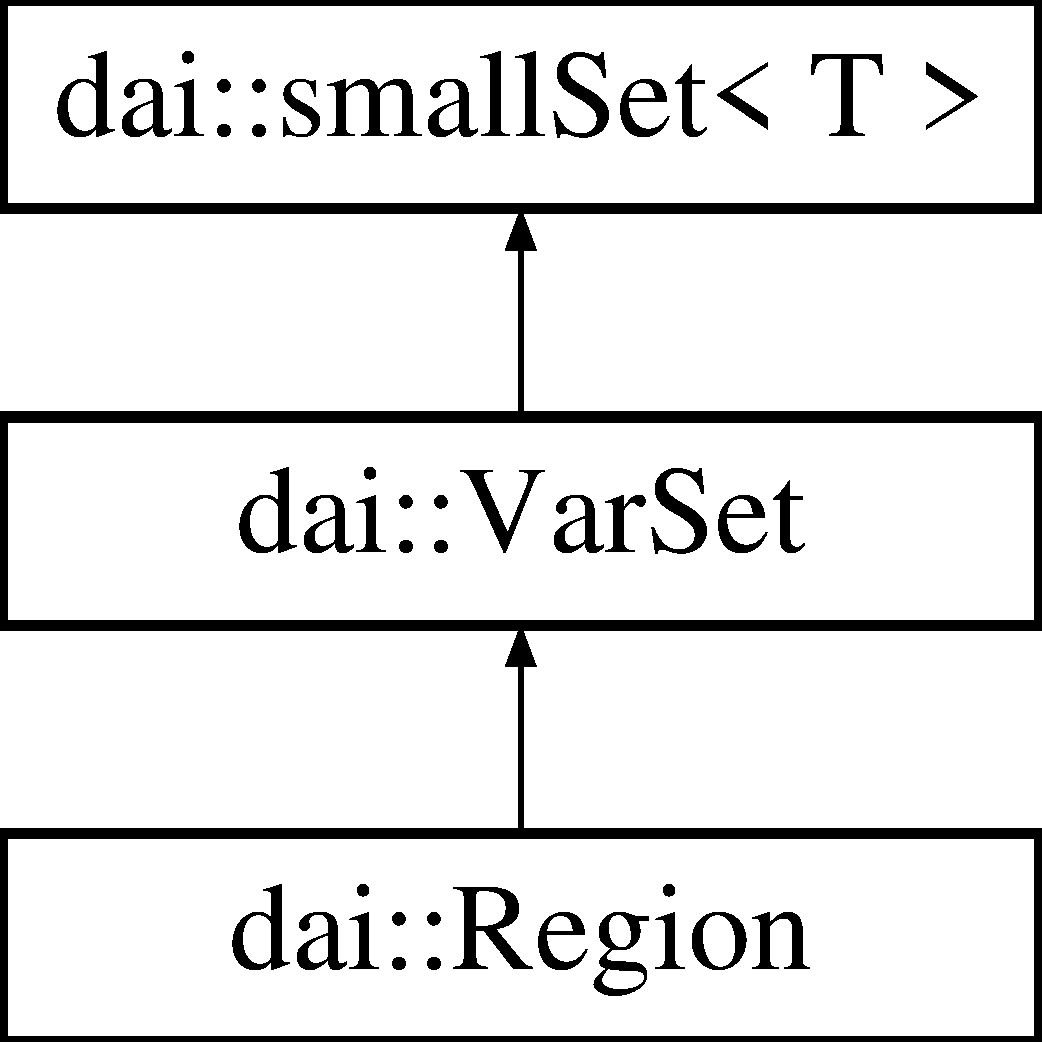
\includegraphics[height=3cm]{classdai_1_1smallSet}
\end{center}
\end{figure}


\subsection{Detailed Description}
\subsubsection*{template$<$typename T$>$ class dai::smallSet$<$ T $>$}

Represents a set (optimized for a small number of elements). 

For sets consisting of a small number of elements, an implementation using an ordered std::vector$<$T$>$ is faster than an implementation using std::set$<$T$>$. The elements should be less-than-comparable. \subsection*{Public Types}
\begin{CompactItemize}
\item 
\hypertarget{classdai_1_1smallSet_103c819872818d14a7234a1f618a815c}{
typedef std::vector$<$ T $>$::\hyperlink{classdai_1_1smallSet_103c819872818d14a7234a1f618a815c}{const\_\-iterator} \hyperlink{classdai_1_1smallSet_103c819872818d14a7234a1f618a815c}{const\_\-iterator}}
\label{classdai_1_1smallSet_103c819872818d14a7234a1f618a815c}

\begin{CompactList}\small\item\em Constant iterator over the elements. \item\end{CompactList}\item 
\hypertarget{classdai_1_1smallSet_254dd4f8cad9c7bce5522e9dbcfc4f49}{
typedef std::vector$<$ T $>$::\hyperlink{classdai_1_1smallSet_254dd4f8cad9c7bce5522e9dbcfc4f49}{iterator} \hyperlink{classdai_1_1smallSet_254dd4f8cad9c7bce5522e9dbcfc4f49}{iterator}}
\label{classdai_1_1smallSet_254dd4f8cad9c7bce5522e9dbcfc4f49}

\begin{CompactList}\small\item\em Iterator over the elements. \item\end{CompactList}\item 
\hypertarget{classdai_1_1smallSet_46882a9010267d41f447feb6aaf65cc1}{
typedef std::vector$<$ T $>$::\hyperlink{classdai_1_1smallSet_46882a9010267d41f447feb6aaf65cc1}{const\_\-reverse\_\-iterator} \hyperlink{classdai_1_1smallSet_46882a9010267d41f447feb6aaf65cc1}{const\_\-reverse\_\-iterator}}
\label{classdai_1_1smallSet_46882a9010267d41f447feb6aaf65cc1}

\begin{CompactList}\small\item\em Constant reverse iterator over the elements. \item\end{CompactList}\item 
\hypertarget{classdai_1_1smallSet_6dea3ee0aa40c4312e6278a7d17f516d}{
typedef std::vector$<$ T $>$::\hyperlink{classdai_1_1smallSet_6dea3ee0aa40c4312e6278a7d17f516d}{reverse\_\-iterator} \hyperlink{classdai_1_1smallSet_6dea3ee0aa40c4312e6278a7d17f516d}{reverse\_\-iterator}}
\label{classdai_1_1smallSet_6dea3ee0aa40c4312e6278a7d17f516d}

\begin{CompactList}\small\item\em Reverse iterator over the elements. \item\end{CompactList}\end{CompactItemize}
\subsection*{Public Member Functions}
\begin{CompactItemize}
\item 
\hypertarget{classdai_1_1smallSet_d352a0a190ca6cf2f512757710a32fa7}{
\hyperlink{classdai_1_1smallSet_d352a0a190ca6cf2f512757710a32fa7}{smallSet} ()}
\label{classdai_1_1smallSet_d352a0a190ca6cf2f512757710a32fa7}

\begin{CompactList}\small\item\em Default constructor. \item\end{CompactList}\item 
\hypertarget{classdai_1_1smallSet_7ac59c3931af4eb31c066e599aa3e388}{
\hyperlink{classdai_1_1smallSet_7ac59c3931af4eb31c066e599aa3e388}{smallSet} (const T \&n)}
\label{classdai_1_1smallSet_7ac59c3931af4eb31c066e599aa3e388}

\begin{CompactList}\small\item\em Construct a \hyperlink{classdai_1_1smallSet}{smallSet} with one element. \item\end{CompactList}\item 
\hypertarget{classdai_1_1smallSet_727f1dd194f77e61c82658fa6b4aff93}{
\hyperlink{classdai_1_1smallSet_727f1dd194f77e61c82658fa6b4aff93}{smallSet} (const T \&n1, const T \&n2)}
\label{classdai_1_1smallSet_727f1dd194f77e61c82658fa6b4aff93}

\begin{CompactList}\small\item\em Construct a \hyperlink{classdai_1_1smallSet}{smallSet} with two elements. \item\end{CompactList}\item 
{\footnotesize template$<$typename Iterator$>$ }\\\hyperlink{classdai_1_1smallSet_54b3816da5edcd6bc664172ef05305a7}{smallSet} (Iterator begin, Iterator end, size\_\-t sizeHint=0)
\begin{CompactList}\small\item\em Construct a \hyperlink{classdai_1_1smallSet}{smallSet} from a range of iterators. \item\end{CompactList}\item 
\hypertarget{classdai_1_1smallSet_5d97d7862890177b0830168f147255ac}{
\hyperlink{classdai_1_1smallSet_5d97d7862890177b0830168f147255ac}{smallSet} (const \hyperlink{classdai_1_1smallSet}{smallSet} \&x)}
\label{classdai_1_1smallSet_5d97d7862890177b0830168f147255ac}

\begin{CompactList}\small\item\em Copy constructor. \item\end{CompactList}\item 
\hypertarget{classdai_1_1smallSet_5cbc0482938044c4ee917844f3ed5842}{
\hyperlink{classdai_1_1smallSet}{smallSet} \& \hyperlink{classdai_1_1smallSet_5cbc0482938044c4ee917844f3ed5842}{operator=} (const \hyperlink{classdai_1_1smallSet}{smallSet} \&x)}
\label{classdai_1_1smallSet_5cbc0482938044c4ee917844f3ed5842}

\begin{CompactList}\small\item\em Assignment operator. \item\end{CompactList}\item 
\hypertarget{classdai_1_1smallSet_daa0dd9b812a6254226965227c0d4828}{
\hyperlink{classdai_1_1smallSet}{smallSet} \hyperlink{classdai_1_1smallSet_daa0dd9b812a6254226965227c0d4828}{operator/} (const \hyperlink{classdai_1_1smallSet}{smallSet} \&ns) const }
\label{classdai_1_1smallSet_daa0dd9b812a6254226965227c0d4828}

\begin{CompactList}\small\item\em Setminus operator: returns all elements in $\ast$this, except those in ns. \item\end{CompactList}\item 
\hypertarget{classdai_1_1smallSet_00de21ede4f1c3d4ba8c3628d67e6446}{
\hyperlink{classdai_1_1smallSet}{smallSet} \hyperlink{classdai_1_1smallSet_00de21ede4f1c3d4ba8c3628d67e6446}{operator$|$} (const \hyperlink{classdai_1_1smallSet}{smallSet} \&ns) const }
\label{classdai_1_1smallSet_00de21ede4f1c3d4ba8c3628d67e6446}

\begin{CompactList}\small\item\em Set-union operator: returns all elements in $\ast$this, plus those in ns. \item\end{CompactList}\item 
\hypertarget{classdai_1_1smallSet_6f436313486360d66a5b9e2ea1a861bd}{
\hyperlink{classdai_1_1smallSet}{smallSet} \hyperlink{classdai_1_1smallSet_6f436313486360d66a5b9e2ea1a861bd}{operator \&} (const \hyperlink{classdai_1_1smallSet}{smallSet} \&ns) const }
\label{classdai_1_1smallSet_6f436313486360d66a5b9e2ea1a861bd}

\begin{CompactList}\small\item\em Set-intersection operator: returns all elements in $\ast$this that are also contained in ns. \item\end{CompactList}\item 
\hypertarget{classdai_1_1smallSet_5a53d38881904f6c7f2e2bbc4489790c}{
\hyperlink{classdai_1_1smallSet}{smallSet} \& \hyperlink{classdai_1_1smallSet_5a53d38881904f6c7f2e2bbc4489790c}{operator/=} (const \hyperlink{classdai_1_1smallSet}{smallSet} \&ns)}
\label{classdai_1_1smallSet_5a53d38881904f6c7f2e2bbc4489790c}

\begin{CompactList}\small\item\em Erases from $\ast$this all elements in ns. \item\end{CompactList}\item 
\hypertarget{classdai_1_1smallSet_8d3db122106f3ea6be80ceafd41316bb}{
\hyperlink{classdai_1_1smallSet}{smallSet} \& \hyperlink{classdai_1_1smallSet_8d3db122106f3ea6be80ceafd41316bb}{operator/=} (const T \&n)}
\label{classdai_1_1smallSet_8d3db122106f3ea6be80ceafd41316bb}

\begin{CompactList}\small\item\em Erases one element. \item\end{CompactList}\item 
\hypertarget{classdai_1_1smallSet_c2e95c8464389c28d989a7e2013999ed}{
\hyperlink{classdai_1_1smallSet}{smallSet} \& \hyperlink{classdai_1_1smallSet_c2e95c8464389c28d989a7e2013999ed}{operator$|$=} (const \hyperlink{classdai_1_1smallSet}{smallSet} \&ns)}
\label{classdai_1_1smallSet_c2e95c8464389c28d989a7e2013999ed}

\begin{CompactList}\small\item\em Adds to $\ast$this all elements in ns. \item\end{CompactList}\item 
\hypertarget{classdai_1_1smallSet_3ab8465276b9f0533b7f641c87dca9e9}{
\hyperlink{classdai_1_1smallSet}{smallSet} \& \hyperlink{classdai_1_1smallSet_3ab8465276b9f0533b7f641c87dca9e9}{operator$|$=} (const T \&n)}
\label{classdai_1_1smallSet_3ab8465276b9f0533b7f641c87dca9e9}

\begin{CompactList}\small\item\em Adds one element. \item\end{CompactList}\item 
\hypertarget{classdai_1_1smallSet_dfcfeeb334b9f46115185c9320ba655b}{
\hyperlink{classdai_1_1smallSet}{smallSet} \& \hyperlink{classdai_1_1smallSet_dfcfeeb334b9f46115185c9320ba655b}{operator \&=} (const \hyperlink{classdai_1_1smallSet}{smallSet} \&ns)}
\label{classdai_1_1smallSet_dfcfeeb334b9f46115185c9320ba655b}

\begin{CompactList}\small\item\em Erases from $\ast$this all elements not in ns. \item\end{CompactList}\item 
\hypertarget{classdai_1_1smallSet_6cd0a2ffbbad14020999cf11199e1e95}{
bool \hyperlink{classdai_1_1smallSet_6cd0a2ffbbad14020999cf11199e1e95}{operator$<$$<$} (const \hyperlink{classdai_1_1smallSet}{smallSet} \&ns) const }
\label{classdai_1_1smallSet_6cd0a2ffbbad14020999cf11199e1e95}

\begin{CompactList}\small\item\em Returns true if $\ast$this is a subset of ns. \item\end{CompactList}\item 
\hypertarget{classdai_1_1smallSet_49518998a31f63cf7a725937da3f2b6e}{
bool \hyperlink{classdai_1_1smallSet_49518998a31f63cf7a725937da3f2b6e}{operator$>$$>$} (const \hyperlink{classdai_1_1smallSet}{smallSet} \&ns) const }
\label{classdai_1_1smallSet_49518998a31f63cf7a725937da3f2b6e}

\begin{CompactList}\small\item\em Returns true if ns is a subset of $\ast$this. \item\end{CompactList}\item 
\hypertarget{classdai_1_1smallSet_c9180f866aa64a6021263a03ec4fab09}{
bool \hyperlink{classdai_1_1smallSet_c9180f866aa64a6021263a03ec4fab09}{intersects} (const \hyperlink{classdai_1_1smallSet}{smallSet} \&ns) const }
\label{classdai_1_1smallSet_c9180f866aa64a6021263a03ec4fab09}

\begin{CompactList}\small\item\em Returns true if $\ast$this and ns contain common elements. \item\end{CompactList}\item 
\hypertarget{classdai_1_1smallSet_82eff80e70adf8c0a541c0a505522b32}{
bool \hyperlink{classdai_1_1smallSet_82eff80e70adf8c0a541c0a505522b32}{contains} (const T \&n) const }
\label{classdai_1_1smallSet_82eff80e70adf8c0a541c0a505522b32}

\begin{CompactList}\small\item\em Returns true if $\ast$this contains the element n. \item\end{CompactList}\item 
\hypertarget{classdai_1_1smallSet_6a14836b896a8bb1901ea79fd45394d0}{
\hyperlink{classdai_1_1smallSet_254dd4f8cad9c7bce5522e9dbcfc4f49}{iterator} \hyperlink{classdai_1_1smallSet_6a14836b896a8bb1901ea79fd45394d0}{begin} ()}
\label{classdai_1_1smallSet_6a14836b896a8bb1901ea79fd45394d0}

\begin{CompactList}\small\item\em Returns iterator that points to the first element. \item\end{CompactList}\item 
\hypertarget{classdai_1_1smallSet_3f0650aa385a3fa8baa1903762815203}{
\hyperlink{classdai_1_1smallSet_103c819872818d14a7234a1f618a815c}{const\_\-iterator} \hyperlink{classdai_1_1smallSet_3f0650aa385a3fa8baa1903762815203}{begin} () const }
\label{classdai_1_1smallSet_3f0650aa385a3fa8baa1903762815203}

\begin{CompactList}\small\item\em Returns constant iterator that points to the first element. \item\end{CompactList}\item 
\hypertarget{classdai_1_1smallSet_9927551b475689ed06d0380f26df8eea}{
\hyperlink{classdai_1_1smallSet_254dd4f8cad9c7bce5522e9dbcfc4f49}{iterator} \hyperlink{classdai_1_1smallSet_9927551b475689ed06d0380f26df8eea}{end} ()}
\label{classdai_1_1smallSet_9927551b475689ed06d0380f26df8eea}

\begin{CompactList}\small\item\em Returns iterator that points beyond the last element. \item\end{CompactList}\item 
\hypertarget{classdai_1_1smallSet_1d4c72c01f605b4bc65c73d1ba259e05}{
\hyperlink{classdai_1_1smallSet_103c819872818d14a7234a1f618a815c}{const\_\-iterator} \hyperlink{classdai_1_1smallSet_1d4c72c01f605b4bc65c73d1ba259e05}{end} () const }
\label{classdai_1_1smallSet_1d4c72c01f605b4bc65c73d1ba259e05}

\begin{CompactList}\small\item\em Returns constant iterator that points beyond the last element. \item\end{CompactList}\item 
\hypertarget{classdai_1_1smallSet_316cf77f22a243a7f68558787b7183c4}{
\hyperlink{classdai_1_1smallSet_6dea3ee0aa40c4312e6278a7d17f516d}{reverse\_\-iterator} \hyperlink{classdai_1_1smallSet_316cf77f22a243a7f68558787b7183c4}{rbegin} ()}
\label{classdai_1_1smallSet_316cf77f22a243a7f68558787b7183c4}

\begin{CompactList}\small\item\em Returns reverse iterator that points to the last element. \item\end{CompactList}\item 
\hypertarget{classdai_1_1smallSet_fe1d0987a5e6df1f488ac59423e60541}{
\hyperlink{classdai_1_1smallSet_46882a9010267d41f447feb6aaf65cc1}{const\_\-reverse\_\-iterator} \hyperlink{classdai_1_1smallSet_fe1d0987a5e6df1f488ac59423e60541}{rbegin} () const }
\label{classdai_1_1smallSet_fe1d0987a5e6df1f488ac59423e60541}

\begin{CompactList}\small\item\em Returns constant reverse iterator that points to the last element. \item\end{CompactList}\item 
\hypertarget{classdai_1_1smallSet_6c13dd3698d76d85f8ed4be564b10f8c}{
\hyperlink{classdai_1_1smallSet_6dea3ee0aa40c4312e6278a7d17f516d}{reverse\_\-iterator} \hyperlink{classdai_1_1smallSet_6c13dd3698d76d85f8ed4be564b10f8c}{rend} ()}
\label{classdai_1_1smallSet_6c13dd3698d76d85f8ed4be564b10f8c}

\begin{CompactList}\small\item\em Returns reverse iterator that points beyond the first element. \item\end{CompactList}\item 
\hypertarget{classdai_1_1smallSet_72f55e13695e993adc7db6fb40b1cd88}{
\hyperlink{classdai_1_1smallSet_46882a9010267d41f447feb6aaf65cc1}{const\_\-reverse\_\-iterator} \hyperlink{classdai_1_1smallSet_72f55e13695e993adc7db6fb40b1cd88}{rend} () const }
\label{classdai_1_1smallSet_72f55e13695e993adc7db6fb40b1cd88}

\begin{CompactList}\small\item\em Returns constant reverse iterator that points beyond the first element. \item\end{CompactList}\item 
\hypertarget{classdai_1_1smallSet_39b00df453666d22331e932d3b7a2f16}{
std::vector$<$ T $>$::size\_\-type \hyperlink{classdai_1_1smallSet_39b00df453666d22331e932d3b7a2f16}{size} () const }
\label{classdai_1_1smallSet_39b00df453666d22331e932d3b7a2f16}

\begin{CompactList}\small\item\em Returns number of elements. \item\end{CompactList}\item 
\hypertarget{classdai_1_1smallSet_b405901de2feb12ff027b973a234a39c}{
bool \hyperlink{classdai_1_1smallSet_b405901de2feb12ff027b973a234a39c}{empty} () const }
\label{classdai_1_1smallSet_b405901de2feb12ff027b973a234a39c}

\begin{CompactList}\small\item\em Returns whether the \hyperlink{classdai_1_1smallSet}{smallSet} is empty. \item\end{CompactList}\end{CompactItemize}
\subsection*{Friends}
\begin{CompactItemize}
\item 
\hypertarget{classdai_1_1smallSet_60606e0d17f55f318f329d556f0c9f80}{
bool \hyperlink{classdai_1_1smallSet_60606e0d17f55f318f329d556f0c9f80}{operator==} (const \hyperlink{classdai_1_1smallSet}{smallSet} \&a, const \hyperlink{classdai_1_1smallSet}{smallSet} \&b)}
\label{classdai_1_1smallSet_60606e0d17f55f318f329d556f0c9f80}

\begin{CompactList}\small\item\em Returns true if the two sets are identical. \item\end{CompactList}\item 
\hypertarget{classdai_1_1smallSet_49e074002843253d59bbe70241e79d84}{
bool \hyperlink{classdai_1_1smallSet_49e074002843253d59bbe70241e79d84}{operator!=} (const \hyperlink{classdai_1_1smallSet}{smallSet} \&a, const \hyperlink{classdai_1_1smallSet}{smallSet} \&b)}
\label{classdai_1_1smallSet_49e074002843253d59bbe70241e79d84}

\begin{CompactList}\small\item\em Returns true if the two sets are not identical. \item\end{CompactList}\item 
\hypertarget{classdai_1_1smallSet_44abfb513a428e283045812964dc64e5}{
bool \hyperlink{classdai_1_1smallSet_44abfb513a428e283045812964dc64e5}{operator$<$} (const \hyperlink{classdai_1_1smallSet}{smallSet} \&a, const \hyperlink{classdai_1_1smallSet}{smallSet} \&b)}
\label{classdai_1_1smallSet_44abfb513a428e283045812964dc64e5}

\begin{CompactList}\small\item\em Lexicographical comparison of elements. \item\end{CompactList}\end{CompactItemize}


\subsection{Constructor \& Destructor Documentation}
\hypertarget{classdai_1_1smallSet_54b3816da5edcd6bc664172ef05305a7}{
\index{dai::smallSet@{dai::smallSet}!smallSet@{smallSet}}
\index{smallSet@{smallSet}!dai::smallSet@{dai::smallSet}}
\subsubsection[smallSet]{\setlength{\rightskip}{0pt plus 5cm}template$<$typename T$>$ template$<$typename Iterator$>$ {\bf dai::smallSet}$<$ T $>$::{\bf smallSet} (Iterator {\em begin}, \/  Iterator {\em end}, \/  size\_\-t {\em sizeHint} = {\tt 0})\hspace{0.3cm}{\tt  \mbox{[}inline\mbox{]}}}}
\label{classdai_1_1smallSet_54b3816da5edcd6bc664172ef05305a7}


Construct a \hyperlink{classdai_1_1smallSet}{smallSet} from a range of iterators. 

\begin{Desc}
\item[Template Parameters:]
\begin{description}
\item[{\em Iterator}]Iterator with value\_\-type T. \end{description}
\end{Desc}
\begin{Desc}
\item[Parameters:]
\begin{description}
\item[{\em begin}]Points to first element to be added. \item[{\em end}]Points just beyond last element to be added. \item[{\em sizeHint}]For efficiency, the number of elements can be speficied by sizeHint. \end{description}
\end{Desc}


The documentation for this class was generated from the following file:\begin{CompactItemize}
\item 
include/dai/\hyperlink{smallset_8h}{smallset.h}\end{CompactItemize}

\hypertarget{classdai_1_1State}{
\section{dai::State Class Reference}
\label{classdai_1_1State}\index{dai::State@{dai::State}}
}
{\tt \#include $<$dai/index.h$>$}



\subsection{Detailed Description}
Contains the joint state of variables within a \hyperlink{classdai_1_1VarSet}{VarSet} and useful things to do with this information. 

This is very similar to a \hyperlink{classdai_1_1MultiFor}{MultiFor}, but tailored for Vars and Varsets. \subsection*{Public Member Functions}
\begin{CompactItemize}
\item 
\hypertarget{classdai_1_1State_ab03f6a5dc8d23f79e0966698f783178}{
\hyperlink{classdai_1_1State_ab03f6a5dc8d23f79e0966698f783178}{State} ()}
\label{classdai_1_1State_ab03f6a5dc8d23f79e0966698f783178}

\begin{CompactList}\small\item\em Default constructor. \item\end{CompactList}\item 
\hypertarget{classdai_1_1State_7c0fe7267ffd7c530283f2444112a162}{
\hyperlink{classdai_1_1State_7c0fe7267ffd7c530283f2444112a162}{State} (const \hyperlink{classdai_1_1VarSet}{VarSet} \&vs)}
\label{classdai_1_1State_7c0fe7267ffd7c530283f2444112a162}

\begin{CompactList}\small\item\em Initialize from \hyperlink{classdai_1_1VarSet}{VarSet}. \item\end{CompactList}\item 
\hypertarget{classdai_1_1State_4ab3583f63942a65c969f4195b508b5b}{
\hyperlink{classdai_1_1State_4ab3583f63942a65c969f4195b508b5b}{State} (const \hyperlink{classdai_1_1State}{State} \&x)}
\label{classdai_1_1State_4ab3583f63942a65c969f4195b508b5b}

\begin{CompactList}\small\item\em Copy constructor. \item\end{CompactList}\item 
\hypertarget{classdai_1_1State_433ced7a70001f4905404c31f09ca9da}{
\hyperlink{classdai_1_1State}{State} \& \hyperlink{classdai_1_1State_433ced7a70001f4905404c31f09ca9da}{operator=} (const \hyperlink{classdai_1_1State}{State} \&x)}
\label{classdai_1_1State_433ced7a70001f4905404c31f09ca9da}

\begin{CompactList}\small\item\em Assignment operator. \item\end{CompactList}\item 
\hypertarget{classdai_1_1State_24d846f8b341073a44191e71b14df219}{
\hyperlink{classdai_1_1State_24d846f8b341073a44191e71b14df219}{operator size\_\-t} () const }
\label{classdai_1_1State_24d846f8b341073a44191e71b14df219}

\begin{CompactList}\small\item\em Return linear state. \item\end{CompactList}\item 
size\_\-t \hyperlink{classdai_1_1State_9d4d70438065731f337963da7bff7e61}{operator()} (const \hyperlink{classdai_1_1Var}{Var} \&n) const 
\item 
size\_\-t \hyperlink{classdai_1_1State_475a14df77520317788c13a3386c3e16}{operator()} (const \hyperlink{classdai_1_1VarSet}{VarSet} \&vs) const 
\item 
\hypertarget{classdai_1_1State_e85f3b76bd05070b75b49fd020f4bff6}{
void \hyperlink{classdai_1_1State_e85f3b76bd05070b75b49fd020f4bff6}{operator++} (int)}
\label{classdai_1_1State_e85f3b76bd05070b75b49fd020f4bff6}

\begin{CompactList}\small\item\em Postfix increment operator. \item\end{CompactList}\item 
\hypertarget{classdai_1_1State_08f7e2c1906e32e95dbad09ad26369d2}{
bool \hyperlink{classdai_1_1State_08f7e2c1906e32e95dbad09ad26369d2}{valid} () const }
\label{classdai_1_1State_08f7e2c1906e32e95dbad09ad26369d2}

\begin{CompactList}\small\item\em Returns true if the current state is valid. \item\end{CompactList}\end{CompactItemize}


\subsection{Member Function Documentation}
\hypertarget{classdai_1_1State_9d4d70438065731f337963da7bff7e61}{
\index{dai::State@{dai::State}!operator()@{operator()}}
\index{operator()@{operator()}!dai::State@{dai::State}}
\subsubsection[operator()]{\setlength{\rightskip}{0pt plus 5cm}size\_\-t dai::State::operator() (const {\bf Var} \& {\em n}) const\hspace{0.3cm}{\tt  \mbox{[}inline\mbox{]}}}}
\label{classdai_1_1State_9d4d70438065731f337963da7bff7e61}


Return state of variable n, or zero if n is not in this \hyperlink{classdai_1_1State}{State} \hypertarget{classdai_1_1State_475a14df77520317788c13a3386c3e16}{
\index{dai::State@{dai::State}!operator()@{operator()}}
\index{operator()@{operator()}!dai::State@{dai::State}}
\subsubsection[operator()]{\setlength{\rightskip}{0pt plus 5cm}size\_\-t dai::State::operator() (const {\bf VarSet} \& {\em vs}) const\hspace{0.3cm}{\tt  \mbox{[}inline\mbox{]}}}}
\label{classdai_1_1State_475a14df77520317788c13a3386c3e16}


Return linear state of variables in varset, setting them to zero if they are not in this \hyperlink{classdai_1_1State}{State} 

The documentation for this class was generated from the following file:\begin{CompactItemize}
\item 
include/dai/\hyperlink{index_8h}{index.h}\end{CompactItemize}

\hypertarget{classdai_1_1TFactor}{
\section{dai::TFactor$<$ T $>$ Class Template Reference}
\label{classdai_1_1TFactor}\index{dai::TFactor@{dai::TFactor}}
}
{\tt \#include $<$dai/factor.h$>$}

Inheritance diagram for dai::TFactor$<$ T $>$::\begin{figure}[H]
\begin{center}
\leavevmode
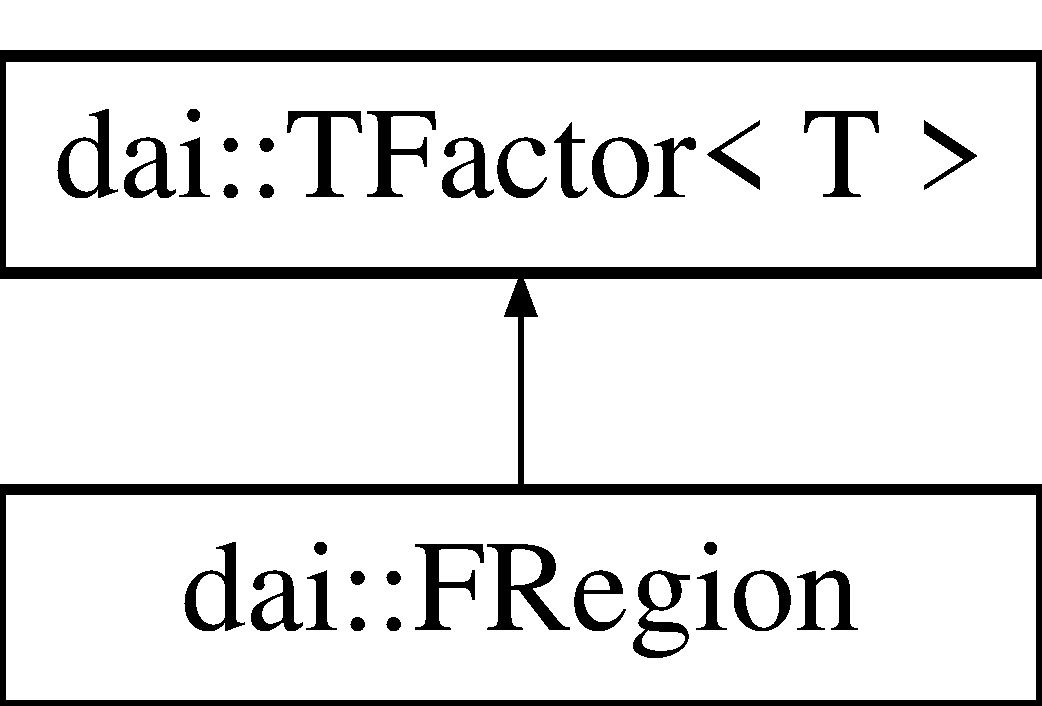
\includegraphics[height=2cm]{classdai_1_1TFactor}
\end{center}
\end{figure}


\subsection{Detailed Description}
\subsubsection*{template$<$typename T$>$ class dai::TFactor$<$ T $>$}

Represents a probability factor. 

A {\em factor\/} is a function of the Cartesian product of the state spaces of some set of variables to the nonnegative real numbers. More formally, if $x_i \in X_i$ for all $i$, then a factor depending on the variables $\{x_i\}$ is a function defined on $\prod_i X_i$ with values in $[0,\infty)$.

A Factor has two components: a \hyperlink{classdai_1_1VarSet}{VarSet}, defining the set of variables that the factor depends on, and a TProb$<$T$>$, containing the values of the factor for all possible joint states of the variables.

\begin{Desc}
\item[Template Parameters:]
\begin{description}
\item[{\em T}]Should be castable from and to double. \end{description}
\end{Desc}
\subsection*{Public Member Functions}
\begin{CompactItemize}
\item 
\hypertarget{classdai_1_1TFactor_da0bedb7a343b45ebcfcbfc0b6c18334}{
\hyperlink{classdai_1_1TFactor_da0bedb7a343b45ebcfcbfc0b6c18334}{TFactor} (\hyperlink{namespacedai_e7d0472fdc89a8635825d01940e91cbf}{Real} p=1.0)}
\label{classdai_1_1TFactor_da0bedb7a343b45ebcfcbfc0b6c18334}

\begin{CompactList}\small\item\em Construct Factor with empty \hyperlink{classdai_1_1VarSet}{VarSet}. \item\end{CompactList}\item 
\hypertarget{classdai_1_1TFactor_8752572e0465b031aa072d3816323509}{
\hyperlink{classdai_1_1TFactor_8752572e0465b031aa072d3816323509}{TFactor} (const \hyperlink{classdai_1_1VarSet}{VarSet} \&ns)}
\label{classdai_1_1TFactor_8752572e0465b031aa072d3816323509}

\begin{CompactList}\small\item\em Construct Factor from \hyperlink{classdai_1_1VarSet}{VarSet}. \item\end{CompactList}\item 
\hypertarget{classdai_1_1TFactor_2d587d2014f55004765685ade322f334}{
\hyperlink{classdai_1_1TFactor_2d587d2014f55004765685ade322f334}{TFactor} (const \hyperlink{classdai_1_1VarSet}{VarSet} \&ns, \hyperlink{namespacedai_e7d0472fdc89a8635825d01940e91cbf}{Real} p)}
\label{classdai_1_1TFactor_2d587d2014f55004765685ade322f334}

\begin{CompactList}\small\item\em Construct Factor from \hyperlink{classdai_1_1VarSet}{VarSet} and initial value. \item\end{CompactList}\item 
\hypertarget{classdai_1_1TFactor_00bb2720d6975adf3c58328be4b96bd4}{
\hyperlink{classdai_1_1TFactor_00bb2720d6975adf3c58328be4b96bd4}{TFactor} (const \hyperlink{classdai_1_1VarSet}{VarSet} \&ns, const \hyperlink{namespacedai_e7d0472fdc89a8635825d01940e91cbf}{Real} $\ast$p)}
\label{classdai_1_1TFactor_00bb2720d6975adf3c58328be4b96bd4}

\begin{CompactList}\small\item\em Construct Factor from \hyperlink{classdai_1_1VarSet}{VarSet} and initial array. \item\end{CompactList}\item 
\hypertarget{classdai_1_1TFactor_e85b382ef05f8f659e13e2b368ad27e2}{
\hyperlink{classdai_1_1TFactor_e85b382ef05f8f659e13e2b368ad27e2}{TFactor} (const \hyperlink{classdai_1_1VarSet}{VarSet} \&ns, const \hyperlink{classdai_1_1TProb}{TProb}$<$ T $>$ \&p)}
\label{classdai_1_1TFactor_e85b382ef05f8f659e13e2b368ad27e2}

\begin{CompactList}\small\item\em Construct Factor from \hyperlink{classdai_1_1VarSet}{VarSet} and TProb$<$T$>$. \item\end{CompactList}\item 
\hypertarget{classdai_1_1TFactor_f3c3586003e78bd4b82fb44b3d06775c}{
\hyperlink{classdai_1_1TFactor_f3c3586003e78bd4b82fb44b3d06775c}{TFactor} (const \hyperlink{classdai_1_1Var}{Var} \&n)}
\label{classdai_1_1TFactor_f3c3586003e78bd4b82fb44b3d06775c}

\begin{CompactList}\small\item\em Construct Factor from \hyperlink{classdai_1_1Var}{Var}. \item\end{CompactList}\item 
\hypertarget{classdai_1_1TFactor_440fb43645f78e6c1471b9b489e74847}{
\hyperlink{classdai_1_1TFactor_440fb43645f78e6c1471b9b489e74847}{TFactor} (const \hyperlink{classdai_1_1TFactor}{TFactor}$<$ T $>$ \&x)}
\label{classdai_1_1TFactor_440fb43645f78e6c1471b9b489e74847}

\begin{CompactList}\small\item\em Copy constructor. \item\end{CompactList}\item 
\hypertarget{classdai_1_1TFactor_bbf1478950a7bc11f9ac4b5e5081e046}{
\hyperlink{classdai_1_1TFactor}{TFactor}$<$ T $>$ \& \hyperlink{classdai_1_1TFactor_bbf1478950a7bc11f9ac4b5e5081e046}{operator=} (const \hyperlink{classdai_1_1TFactor}{TFactor}$<$ T $>$ \&x)}
\label{classdai_1_1TFactor_bbf1478950a7bc11f9ac4b5e5081e046}

\begin{CompactList}\small\item\em Assignment operator. \item\end{CompactList}\item 
\hypertarget{classdai_1_1TFactor_c742180c0abe1be45fbf3208f7014a1b}{
const \hyperlink{classdai_1_1TProb}{TProb}$<$ T $>$ \& \hyperlink{classdai_1_1TFactor_c742180c0abe1be45fbf3208f7014a1b}{p} () const }
\label{classdai_1_1TFactor_c742180c0abe1be45fbf3208f7014a1b}

\begin{CompactList}\small\item\em Returns const reference to probability entries. \item\end{CompactList}\item 
\hypertarget{classdai_1_1TFactor_ba85b145db1c3b72978e11fb385659e1}{
\hyperlink{classdai_1_1TProb}{TProb}$<$ T $>$ \& \hyperlink{classdai_1_1TFactor_ba85b145db1c3b72978e11fb385659e1}{p} ()}
\label{classdai_1_1TFactor_ba85b145db1c3b72978e11fb385659e1}

\begin{CompactList}\small\item\em Returns reference to probability entries. \item\end{CompactList}\item 
\hypertarget{classdai_1_1TFactor_54c575d53b8c8a6a03c26c8cdc600ce4}{
const \hyperlink{classdai_1_1VarSet}{VarSet} \& \hyperlink{classdai_1_1TFactor_54c575d53b8c8a6a03c26c8cdc600ce4}{vars} () const }
\label{classdai_1_1TFactor_54c575d53b8c8a6a03c26c8cdc600ce4}

\begin{CompactList}\small\item\em Returns const reference to variables. \item\end{CompactList}\item 
\hypertarget{classdai_1_1TFactor_57d676927a5dcacbef47f564c46bf128}{
size\_\-t \hyperlink{classdai_1_1TFactor_57d676927a5dcacbef47f564c46bf128}{states} () const }
\label{classdai_1_1TFactor_57d676927a5dcacbef47f564c46bf128}

\begin{CompactList}\small\item\em Returns the number of possible joint states of the variables. \item\end{CompactList}\item 
\hypertarget{classdai_1_1TFactor_22a12143c01d05a1e70ca3f92ec42595}{
T \hyperlink{classdai_1_1TFactor_22a12143c01d05a1e70ca3f92ec42595}{operator\mbox{[}$\,$\mbox{]}} (size\_\-t i) const }
\label{classdai_1_1TFactor_22a12143c01d05a1e70ca3f92ec42595}

\begin{CompactList}\small\item\em Returns a copy of the i'th probability value. \item\end{CompactList}\item 
\hypertarget{classdai_1_1TFactor_8be917166f0f32f2da09e09fc5fa2651}{
T \& \hyperlink{classdai_1_1TFactor_8be917166f0f32f2da09e09fc5fa2651}{operator\mbox{[}$\,$\mbox{]}} (size\_\-t i)}
\label{classdai_1_1TFactor_8be917166f0f32f2da09e09fc5fa2651}

\begin{CompactList}\small\item\em Returns a reference to the i'th probability value. \item\end{CompactList}\item 
\hypertarget{classdai_1_1TFactor_949ed2c4aefdf1aadfe33d0c2dac89b3}{
\hyperlink{classdai_1_1TFactor}{TFactor}$<$ T $>$ \& \hyperlink{classdai_1_1TFactor_949ed2c4aefdf1aadfe33d0c2dac89b3}{fill} (T p)}
\label{classdai_1_1TFactor_949ed2c4aefdf1aadfe33d0c2dac89b3}

\begin{CompactList}\small\item\em Sets all probability entries to p. \item\end{CompactList}\item 
\hypertarget{classdai_1_1TFactor_f52a4ee1544b4e628390918239b7bc1b}{
\hyperlink{classdai_1_1TFactor}{TFactor}$<$ T $>$ \& \hyperlink{classdai_1_1TFactor_f52a4ee1544b4e628390918239b7bc1b}{randomize} ()}
\label{classdai_1_1TFactor_f52a4ee1544b4e628390918239b7bc1b}

\begin{CompactList}\small\item\em Fills all probability entries with random values. \item\end{CompactList}\item 
\hypertarget{classdai_1_1TFactor_cf5fc0dd70aa8a7e7c2da3b3acdf6747}{
\hyperlink{classdai_1_1TFactor}{TFactor}$<$ T $>$ \hyperlink{classdai_1_1TFactor_cf5fc0dd70aa8a7e7c2da3b3acdf6747}{operator$\ast$} (T x) const }
\label{classdai_1_1TFactor_cf5fc0dd70aa8a7e7c2da3b3acdf6747}

\begin{CompactList}\small\item\em Returns product of $\ast$this with x. \item\end{CompactList}\item 
\hypertarget{classdai_1_1TFactor_e8a33191e3bc570737ff29e77966c33e}{
\hyperlink{classdai_1_1TFactor}{TFactor}$<$ T $>$ \& \hyperlink{classdai_1_1TFactor_e8a33191e3bc570737ff29e77966c33e}{operator$\ast$=} (T x)}
\label{classdai_1_1TFactor_e8a33191e3bc570737ff29e77966c33e}

\begin{CompactList}\small\item\em Multiplies each probability entry with x. \item\end{CompactList}\item 
\hypertarget{classdai_1_1TFactor_35fd7313a64a83aba0cd087d1b60289d}{
\hyperlink{classdai_1_1TFactor}{TFactor}$<$ T $>$ \hyperlink{classdai_1_1TFactor_35fd7313a64a83aba0cd087d1b60289d}{operator/} (T x) const }
\label{classdai_1_1TFactor_35fd7313a64a83aba0cd087d1b60289d}

\begin{CompactList}\small\item\em Returns quotient of $\ast$this with x. \item\end{CompactList}\item 
\hypertarget{classdai_1_1TFactor_45c34bf15cc9b37e5c0718d96d9d2c1a}{
\hyperlink{classdai_1_1TFactor}{TFactor}$<$ T $>$ \& \hyperlink{classdai_1_1TFactor_45c34bf15cc9b37e5c0718d96d9d2c1a}{operator/=} (T x)}
\label{classdai_1_1TFactor_45c34bf15cc9b37e5c0718d96d9d2c1a}

\begin{CompactList}\small\item\em Divides each probability entry by x. \item\end{CompactList}\item 
\hypertarget{classdai_1_1TFactor_53f052f85f5274b783eaa1ecd31a6b35}{
\hyperlink{classdai_1_1TFactor}{TFactor}$<$ T $>$ \hyperlink{classdai_1_1TFactor_53f052f85f5274b783eaa1ecd31a6b35}{operator$\ast$} (const \hyperlink{classdai_1_1TFactor}{TFactor}$<$ T $>$ \&Q) const }
\label{classdai_1_1TFactor_53f052f85f5274b783eaa1ecd31a6b35}

\begin{CompactList}\small\item\em Returns product of $\ast$this with another Factor. \item\end{CompactList}\item 
\hypertarget{classdai_1_1TFactor_f5894eb556d2c440774e650102207d80}{
\hyperlink{classdai_1_1TFactor}{TFactor}$<$ T $>$ \hyperlink{classdai_1_1TFactor_f5894eb556d2c440774e650102207d80}{operator/} (const \hyperlink{classdai_1_1TFactor}{TFactor}$<$ T $>$ \&Q) const }
\label{classdai_1_1TFactor_f5894eb556d2c440774e650102207d80}

\begin{CompactList}\small\item\em Returns quotient of $\ast$this with another Factor. \item\end{CompactList}\item 
\hypertarget{classdai_1_1TFactor_914cb4b11fdffa4daaebf645f539d5d1}{
\hyperlink{classdai_1_1TFactor}{TFactor}$<$ T $>$ \& \hyperlink{classdai_1_1TFactor_914cb4b11fdffa4daaebf645f539d5d1}{operator$\ast$=} (const \hyperlink{classdai_1_1TFactor}{TFactor}$<$ T $>$ \&Q)}
\label{classdai_1_1TFactor_914cb4b11fdffa4daaebf645f539d5d1}

\begin{CompactList}\small\item\em Multiplies $\ast$this with another Factor. \item\end{CompactList}\item 
\hypertarget{classdai_1_1TFactor_c5ac7c898b536ecbed7a1f58e3899cdb}{
\hyperlink{classdai_1_1TFactor}{TFactor}$<$ T $>$ \& \hyperlink{classdai_1_1TFactor_c5ac7c898b536ecbed7a1f58e3899cdb}{operator/=} (const \hyperlink{classdai_1_1TFactor}{TFactor}$<$ T $>$ \&Q)}
\label{classdai_1_1TFactor_c5ac7c898b536ecbed7a1f58e3899cdb}

\begin{CompactList}\small\item\em Divides $\ast$this by another Factor. \item\end{CompactList}\item 
\hypertarget{classdai_1_1TFactor_5db00c03b427e577bab01646c451ae23}{
\hyperlink{classdai_1_1TFactor}{TFactor}$<$ T $>$ \hyperlink{classdai_1_1TFactor_5db00c03b427e577bab01646c451ae23}{operator+} (const \hyperlink{classdai_1_1TFactor}{TFactor}$<$ T $>$ \&Q) const }
\label{classdai_1_1TFactor_5db00c03b427e577bab01646c451ae23}

\begin{CompactList}\small\item\em Returns sum of $\ast$this and another Factor (their \hyperlink{classdai_1_1TFactor_54c575d53b8c8a6a03c26c8cdc600ce4}{vars()} should be identical). \item\end{CompactList}\item 
\hypertarget{classdai_1_1TFactor_36cd699efe9bcce52fb21d6a3eb7024a}{
\hyperlink{classdai_1_1TFactor}{TFactor}$<$ T $>$ \hyperlink{classdai_1_1TFactor_36cd699efe9bcce52fb21d6a3eb7024a}{operator-} (const \hyperlink{classdai_1_1TFactor}{TFactor}$<$ T $>$ \&Q) const }
\label{classdai_1_1TFactor_36cd699efe9bcce52fb21d6a3eb7024a}

\begin{CompactList}\small\item\em Returns difference of $\ast$this and another Factor (their \hyperlink{classdai_1_1TFactor_54c575d53b8c8a6a03c26c8cdc600ce4}{vars()} should be identical). \item\end{CompactList}\item 
\hypertarget{classdai_1_1TFactor_098a7c22159f23dead9e16ad3dff1e90}{
\hyperlink{classdai_1_1TFactor}{TFactor}$<$ T $>$ \& \hyperlink{classdai_1_1TFactor_098a7c22159f23dead9e16ad3dff1e90}{operator+=} (const \hyperlink{classdai_1_1TFactor}{TFactor}$<$ T $>$ \&Q)}
\label{classdai_1_1TFactor_098a7c22159f23dead9e16ad3dff1e90}

\begin{CompactList}\small\item\em Adds another Factor to $\ast$this (their \hyperlink{classdai_1_1TFactor_54c575d53b8c8a6a03c26c8cdc600ce4}{vars()} should be identical). \item\end{CompactList}\item 
\hypertarget{classdai_1_1TFactor_a6dd7ae3384f6f329e2cb3c3fa31e514}{
\hyperlink{classdai_1_1TFactor}{TFactor}$<$ T $>$ \& \hyperlink{classdai_1_1TFactor_a6dd7ae3384f6f329e2cb3c3fa31e514}{operator-=} (const \hyperlink{classdai_1_1TFactor}{TFactor}$<$ T $>$ \&Q)}
\label{classdai_1_1TFactor_a6dd7ae3384f6f329e2cb3c3fa31e514}

\begin{CompactList}\small\item\em Subtracts another Factor from $\ast$this (their \hyperlink{classdai_1_1TFactor_54c575d53b8c8a6a03c26c8cdc600ce4}{vars()} should be identical). \item\end{CompactList}\item 
\hypertarget{classdai_1_1TFactor_fda1418de5d67a6ba004eaea3ef66f77}{
\hyperlink{classdai_1_1TFactor}{TFactor}$<$ T $>$ \& \hyperlink{classdai_1_1TFactor_fda1418de5d67a6ba004eaea3ef66f77}{operator+=} (T q)}
\label{classdai_1_1TFactor_fda1418de5d67a6ba004eaea3ef66f77}

\begin{CompactList}\small\item\em Adds scalar to $\ast$this. \item\end{CompactList}\item 
\hypertarget{classdai_1_1TFactor_d74386483d4f28011ddc962db443e3aa}{
\hyperlink{classdai_1_1TFactor}{TFactor}$<$ T $>$ \& \hyperlink{classdai_1_1TFactor_d74386483d4f28011ddc962db443e3aa}{operator-=} (T q)}
\label{classdai_1_1TFactor_d74386483d4f28011ddc962db443e3aa}

\begin{CompactList}\small\item\em Subtracts scalar from $\ast$this. \item\end{CompactList}\item 
\hypertarget{classdai_1_1TFactor_3c2f95c6fddf19bd871a89f419991c08}{
\hyperlink{classdai_1_1TFactor}{TFactor}$<$ T $>$ \hyperlink{classdai_1_1TFactor_3c2f95c6fddf19bd871a89f419991c08}{operator+} (T q) const }
\label{classdai_1_1TFactor_3c2f95c6fddf19bd871a89f419991c08}

\begin{CompactList}\small\item\em Returns sum of $\ast$this and a scalar. \item\end{CompactList}\item 
\hypertarget{classdai_1_1TFactor_171e3bab13b2cd054e8ce1eb97be1112}{
\hyperlink{classdai_1_1TFactor}{TFactor}$<$ T $>$ \hyperlink{classdai_1_1TFactor_171e3bab13b2cd054e8ce1eb97be1112}{operator-} (T q) const }
\label{classdai_1_1TFactor_171e3bab13b2cd054e8ce1eb97be1112}

\begin{CompactList}\small\item\em Returns difference of $\ast$this with a scalar. \item\end{CompactList}\item 
\hypertarget{classdai_1_1TFactor_9b87c70ab153534d5cdbbdba6aaa7921}{
\hyperlink{classdai_1_1TFactor}{TFactor}$<$ T $>$ \hyperlink{classdai_1_1TFactor_9b87c70ab153534d5cdbbdba6aaa7921}{operator$^\wedge$} (\hyperlink{namespacedai_e7d0472fdc89a8635825d01940e91cbf}{Real} a) const }
\label{classdai_1_1TFactor_9b87c70ab153534d5cdbbdba6aaa7921}

\begin{CompactList}\small\item\em Returns $\ast$this raised to some power. \item\end{CompactList}\item 
\hypertarget{classdai_1_1TFactor_4cd8337eb9ae63205692a28435322d3b}{
\hyperlink{classdai_1_1TFactor}{TFactor}$<$ T $>$ \& \hyperlink{classdai_1_1TFactor_4cd8337eb9ae63205692a28435322d3b}{operator$^\wedge$=} (\hyperlink{namespacedai_e7d0472fdc89a8635825d01940e91cbf}{Real} a)}
\label{classdai_1_1TFactor_4cd8337eb9ae63205692a28435322d3b}

\begin{CompactList}\small\item\em Raises $\ast$this to some power. \item\end{CompactList}\item 
\hypertarget{classdai_1_1TFactor_8ab0a98ebf512cd5a27e6a2618ed4353}{
\hyperlink{classdai_1_1TFactor}{TFactor}$<$ T $>$ \& \hyperlink{classdai_1_1TFactor_8ab0a98ebf512cd5a27e6a2618ed4353}{makeZero} (\hyperlink{namespacedai_e7d0472fdc89a8635825d01940e91cbf}{Real} epsilon)}
\label{classdai_1_1TFactor_8ab0a98ebf512cd5a27e6a2618ed4353}

\begin{CompactList}\small\item\em Sets all entries that are smaller than epsilon to zero. \item\end{CompactList}\item 
\hypertarget{classdai_1_1TFactor_731c8683fc17269c4bf3f7b52e0c4b40}{
\hyperlink{classdai_1_1TFactor}{TFactor}$<$ T $>$ \& \hyperlink{classdai_1_1TFactor_731c8683fc17269c4bf3f7b52e0c4b40}{makePositive} (\hyperlink{namespacedai_e7d0472fdc89a8635825d01940e91cbf}{Real} epsilon)}
\label{classdai_1_1TFactor_731c8683fc17269c4bf3f7b52e0c4b40}

\begin{CompactList}\small\item\em Sets all entries that are smaller than epsilon to epsilon. \item\end{CompactList}\item 
\hypertarget{classdai_1_1TFactor_de249c30222894e50170a834aca6d708}{
\hyperlink{classdai_1_1TFactor}{TFactor}$<$ T $>$ \hyperlink{classdai_1_1TFactor_de249c30222894e50170a834aca6d708}{inverse} () const }
\label{classdai_1_1TFactor_de249c30222894e50170a834aca6d708}

\begin{CompactList}\small\item\em Returns inverse of $\ast$this. \item\end{CompactList}\item 
\hypertarget{classdai_1_1TFactor_1747eaa67d359d34d9221d368753ecdf}{
\hyperlink{classdai_1_1TFactor}{TFactor}$<$ T $>$ \hyperlink{classdai_1_1TFactor_1747eaa67d359d34d9221d368753ecdf}{divided\_\-by} (const \hyperlink{classdai_1_1TFactor}{TFactor}$<$ T $>$ \&denom) const }
\label{classdai_1_1TFactor_1747eaa67d359d34d9221d368753ecdf}

\begin{CompactList}\small\item\em Returns $\ast$this divided by another Factor. \item\end{CompactList}\item 
\hypertarget{classdai_1_1TFactor_275c1fd149c36a9e67256d21ad97dde1}{
\hyperlink{classdai_1_1TFactor}{TFactor}$<$ T $>$ \& \hyperlink{classdai_1_1TFactor_275c1fd149c36a9e67256d21ad97dde1}{divide} (const \hyperlink{classdai_1_1TFactor}{TFactor}$<$ T $>$ \&denom)}
\label{classdai_1_1TFactor_275c1fd149c36a9e67256d21ad97dde1}

\begin{CompactList}\small\item\em Divides $\ast$this by another Factor. \item\end{CompactList}\item 
\hypertarget{classdai_1_1TFactor_284a962817d33244c261be5d7f0159ca}{
\hyperlink{classdai_1_1TFactor}{TFactor}$<$ T $>$ \hyperlink{classdai_1_1TFactor_284a962817d33244c261be5d7f0159ca}{exp} () const }
\label{classdai_1_1TFactor_284a962817d33244c261be5d7f0159ca}

\begin{CompactList}\small\item\em Returns exp of $\ast$this. \item\end{CompactList}\item 
\hypertarget{classdai_1_1TFactor_fa3435d85ca11399aba42c63a008765a}{
\hyperlink{classdai_1_1TFactor}{TFactor}$<$ T $>$ \hyperlink{classdai_1_1TFactor_fa3435d85ca11399aba42c63a008765a}{abs} () const }
\label{classdai_1_1TFactor_fa3435d85ca11399aba42c63a008765a}

\begin{CompactList}\small\item\em Returns absolute value of $\ast$this. \item\end{CompactList}\item 
\hypertarget{classdai_1_1TFactor_fbbcf3a69afa5fb3bde1f5a8180860c6}{
\hyperlink{classdai_1_1TFactor}{TFactor}$<$ T $>$ \hyperlink{classdai_1_1TFactor_fbbcf3a69afa5fb3bde1f5a8180860c6}{log} () const }
\label{classdai_1_1TFactor_fbbcf3a69afa5fb3bde1f5a8180860c6}

\begin{CompactList}\small\item\em Returns logarithm of $\ast$this. \item\end{CompactList}\item 
\hypertarget{classdai_1_1TFactor_72b37d26ccac6edb39e71209bb675ba7}{
\hyperlink{classdai_1_1TFactor}{TFactor}$<$ T $>$ \hyperlink{classdai_1_1TFactor_72b37d26ccac6edb39e71209bb675ba7}{log0} () const }
\label{classdai_1_1TFactor_72b37d26ccac6edb39e71209bb675ba7}

\begin{CompactList}\small\item\em Returns logarithm of $\ast$this (defining log(0)=0). \item\end{CompactList}\item 
\hypertarget{classdai_1_1TFactor_c69a94a4d055c3cac107b2a55bb42944}{
T \hyperlink{classdai_1_1TFactor_c69a94a4d055c3cac107b2a55bb42944}{normalize} (typename \hyperlink{classdai_1_1TProb_31d9206096f52574dbd24cbb2502080c}{Prob::NormType} norm=Prob::NORMPROB)}
\label{classdai_1_1TFactor_c69a94a4d055c3cac107b2a55bb42944}

\begin{CompactList}\small\item\em Normalizes $\ast$this Factor. \item\end{CompactList}\item 
\hypertarget{classdai_1_1TFactor_df4740f4558ed9bc27029c0c362923e2}{
\hyperlink{classdai_1_1TFactor}{TFactor}$<$ T $>$ \hyperlink{classdai_1_1TFactor_df4740f4558ed9bc27029c0c362923e2}{normalized} (typename \hyperlink{classdai_1_1TProb_31d9206096f52574dbd24cbb2502080c}{Prob::NormType} norm=Prob::NORMPROB) const }
\label{classdai_1_1TFactor_df4740f4558ed9bc27029c0c362923e2}

\begin{CompactList}\small\item\em Returns a normalized copy of $\ast$this. \item\end{CompactList}\item 
\hypertarget{classdai_1_1TFactor_7cc9e6bca2b9c187f8d907942264508f}{
\hyperlink{classdai_1_1TFactor}{Factor} \hyperlink{classdai_1_1TFactor_7cc9e6bca2b9c187f8d907942264508f}{slice} (const \hyperlink{classdai_1_1VarSet}{VarSet} \&ns, size\_\-t ns\_\-state) const }
\label{classdai_1_1TFactor_7cc9e6bca2b9c187f8d907942264508f}

\begin{CompactList}\small\item\em Returns a slice of this factor, where the subset ns is in state ns\_\-state. \item\end{CompactList}\item 
\hypertarget{classdai_1_1TFactor_f90e2a8a5ef94809ae8905e19fc523e4}{
\hyperlink{classdai_1_1TFactor}{TFactor}$<$ T $>$ \hyperlink{classdai_1_1TFactor_f90e2a8a5ef94809ae8905e19fc523e4}{partSum} (const \hyperlink{classdai_1_1VarSet}{VarSet} \&ns) const }
\label{classdai_1_1TFactor_f90e2a8a5ef94809ae8905e19fc523e4}

\begin{CompactList}\small\item\em Returns unnormalized marginal; ns should be a subset of \hyperlink{classdai_1_1TFactor_54c575d53b8c8a6a03c26c8cdc600ce4}{vars()}. \item\end{CompactList}\item 
\hypertarget{classdai_1_1TFactor_692df5b8aed5f6faeb60e076624d5854}{
\hyperlink{classdai_1_1TFactor}{TFactor}$<$ T $>$ \hyperlink{classdai_1_1TFactor_692df5b8aed5f6faeb60e076624d5854}{marginal} (const \hyperlink{classdai_1_1VarSet}{VarSet} \&ns, bool normed=true) const }
\label{classdai_1_1TFactor_692df5b8aed5f6faeb60e076624d5854}

\begin{CompactList}\small\item\em Returns (normalized by default) marginal; ns should be a subset of \hyperlink{classdai_1_1TFactor_54c575d53b8c8a6a03c26c8cdc600ce4}{vars()}. \item\end{CompactList}\item 
\hypertarget{classdai_1_1TFactor_fd92183f10a4214341ce771b02f8744d}{
\hyperlink{classdai_1_1TFactor}{TFactor}$<$ T $>$ \hyperlink{classdai_1_1TFactor_fd92183f10a4214341ce771b02f8744d}{notSum} (const \hyperlink{classdai_1_1VarSet}{VarSet} \&ns) const }
\label{classdai_1_1TFactor_fd92183f10a4214341ce771b02f8744d}

\begin{CompactList}\small\item\em Sums out all variables except those in ns. \item\end{CompactList}\item 
\hypertarget{classdai_1_1TFactor_81c344b9e204bb57aaca92c281aa7dd3}{
\hyperlink{classdai_1_1TFactor}{TFactor}$<$ T $>$ \hyperlink{classdai_1_1TFactor_81c344b9e204bb57aaca92c281aa7dd3}{embed} (const \hyperlink{classdai_1_1VarSet}{VarSet} \&ns) const }
\label{classdai_1_1TFactor_81c344b9e204bb57aaca92c281aa7dd3}

\begin{CompactList}\small\item\em Embeds this factor in a larger \hyperlink{classdai_1_1VarSet}{VarSet}. \item\end{CompactList}\item 
\hypertarget{classdai_1_1TFactor_dafb816c6d9f93ceea858709391841d2}{
bool \hyperlink{classdai_1_1TFactor_dafb816c6d9f93ceea858709391841d2}{hasNaNs} () const }
\label{classdai_1_1TFactor_dafb816c6d9f93ceea858709391841d2}

\begin{CompactList}\small\item\em Returns true if $\ast$this has NANs. \item\end{CompactList}\item 
\hypertarget{classdai_1_1TFactor_7353d87f8a1d4c6c24b9cc5de7b18219}{
bool \hyperlink{classdai_1_1TFactor_7353d87f8a1d4c6c24b9cc5de7b18219}{hasNegatives} () const }
\label{classdai_1_1TFactor_7353d87f8a1d4c6c24b9cc5de7b18219}

\begin{CompactList}\small\item\em Returns true if $\ast$this has negative entries. \item\end{CompactList}\item 
\hypertarget{classdai_1_1TFactor_aff9f62e6ef5792a459946cd81bd35af}{
T \hyperlink{classdai_1_1TFactor_aff9f62e6ef5792a459946cd81bd35af}{totalSum} () const }
\label{classdai_1_1TFactor_aff9f62e6ef5792a459946cd81bd35af}

\begin{CompactList}\small\item\em Returns total sum of probability entries. \item\end{CompactList}\item 
\hypertarget{classdai_1_1TFactor_8e67b044dfaebf20c77031a2378e65f5}{
T \hyperlink{classdai_1_1TFactor_8e67b044dfaebf20c77031a2378e65f5}{maxAbs} () const }
\label{classdai_1_1TFactor_8e67b044dfaebf20c77031a2378e65f5}

\begin{CompactList}\small\item\em Returns maximum absolute value of probability entries. \item\end{CompactList}\item 
\hypertarget{classdai_1_1TFactor_160c82f59a3202180025853a9e5caaa5}{
T \hyperlink{classdai_1_1TFactor_160c82f59a3202180025853a9e5caaa5}{maxVal} () const }
\label{classdai_1_1TFactor_160c82f59a3202180025853a9e5caaa5}

\begin{CompactList}\small\item\em Returns maximum value of probability entries. \item\end{CompactList}\item 
\hypertarget{classdai_1_1TFactor_891e98fd0cd9f65f945eb5733c6c3e9f}{
T \hyperlink{classdai_1_1TFactor_891e98fd0cd9f65f945eb5733c6c3e9f}{minVal} () const }
\label{classdai_1_1TFactor_891e98fd0cd9f65f945eb5733c6c3e9f}

\begin{CompactList}\small\item\em Returns minimum value of probability entries. \item\end{CompactList}\item 
\hypertarget{classdai_1_1TFactor_948c0013f741040ecdcad7da53377268}{
\hyperlink{namespacedai_e7d0472fdc89a8635825d01940e91cbf}{Real} \hyperlink{classdai_1_1TFactor_948c0013f741040ecdcad7da53377268}{entropy} () const }
\label{classdai_1_1TFactor_948c0013f741040ecdcad7da53377268}

\begin{CompactList}\small\item\em Returns entropy of $\ast$this. \item\end{CompactList}\item 
\hypertarget{classdai_1_1TFactor_4908ad29222b60d669d234d0805605b8}{
T \hyperlink{classdai_1_1TFactor_4908ad29222b60d669d234d0805605b8}{strength} (const \hyperlink{classdai_1_1Var}{Var} \&i, const \hyperlink{classdai_1_1Var}{Var} \&j) const }
\label{classdai_1_1TFactor_4908ad29222b60d669d234d0805605b8}

\begin{CompactList}\small\item\em Returns strength of $\ast$this, between variables i and j, using (52) of \mbox{[}\hyperlink{Bibliography_MoK07b}{MoK07b}\mbox{]}. \item\end{CompactList}\end{CompactItemize}


The documentation for this class was generated from the following file:\begin{CompactItemize}
\item 
include/dai/\hyperlink{factor_8h}{factor.h}\end{CompactItemize}

\hypertarget{classdai_1_1TProb}{
\section{dai::TProb$<$ T $>$ Class Template Reference}
\label{classdai_1_1TProb}\index{dai::TProb@{dai::TProb}}
}
{\tt \#include $<$dai/prob.h$>$}



\subsection{Detailed Description}
\subsubsection*{template$<$typename T$>$ class dai::TProb$<$ T $>$}

Represents a probability measure on a finite outcome space (i.e., corresponding to a discrete random variable). 

It is implemented as a std::vector$<$T$>$ but adds a convenient interface. It is not necessarily normalized at all times. \begin{Desc}
\item[Template Parameters:]
\begin{description}
\item[{\em T}]Should be castable from and to double. \end{description}
\end{Desc}
\subsection*{Public Types}
\begin{CompactItemize}
\item 
enum \hyperlink{classdai_1_1TProb_31d9206096f52574dbd24cbb2502080c}{NormType} \{ \textbf{NORMPROB}, 
\textbf{NORMLINF}
 \}
\begin{CompactList}\small\item\em Enumerates different ways of normalizing a probability measure. \item\end{CompactList}\item 
enum \hyperlink{classdai_1_1TProb_492487fd71f6e87673853e5e2fda2f27}{DistType} \{ \textbf{DISTL1}, 
\textbf{DISTLINF}, 
\textbf{DISTTV}, 
\textbf{DISTKL}
 \}
\begin{CompactList}\small\item\em Enumerates different distance measures between probability measures. \item\end{CompactList}\end{CompactItemize}
\subsection*{Public Member Functions}
\begin{CompactItemize}
\item 
\hypertarget{classdai_1_1TProb_81f9393fa860a6bb005c8286bf9aceab}{
\hyperlink{classdai_1_1TProb_81f9393fa860a6bb005c8286bf9aceab}{TProb} ()}
\label{classdai_1_1TProb_81f9393fa860a6bb005c8286bf9aceab}

\begin{CompactList}\small\item\em Default constructor. \item\end{CompactList}\item 
\hypertarget{classdai_1_1TProb_851cd9b5be495df487fb177b0e06a1dd}{
\hyperlink{classdai_1_1TProb_851cd9b5be495df487fb177b0e06a1dd}{TProb} (size\_\-t n)}
\label{classdai_1_1TProb_851cd9b5be495df487fb177b0e06a1dd}

\begin{CompactList}\small\item\em Construct uniform distribution of given length. \item\end{CompactList}\item 
\hypertarget{classdai_1_1TProb_de3ff7ee6617e3ae59dd8c4e4fb146f3}{
\hyperlink{classdai_1_1TProb_de3ff7ee6617e3ae59dd8c4e4fb146f3}{TProb} (size\_\-t n, \hyperlink{namespacedai_e7d0472fdc89a8635825d01940e91cbf}{Real} p)}
\label{classdai_1_1TProb_de3ff7ee6617e3ae59dd8c4e4fb146f3}

\begin{CompactList}\small\item\em Construct from given length and initial value. \item\end{CompactList}\item 
\hypertarget{classdai_1_1TProb_b139b37cc0533d119a55054a574987a5}{
\hyperlink{classdai_1_1TProb_b139b37cc0533d119a55054a574987a5}{TProb} (size\_\-t n, const \hyperlink{namespacedai_e7d0472fdc89a8635825d01940e91cbf}{Real} $\ast$p)}
\label{classdai_1_1TProb_b139b37cc0533d119a55054a574987a5}

\begin{CompactList}\small\item\em Construct from given length and initial array. \item\end{CompactList}\item 
\hypertarget{classdai_1_1TProb_408eb13e9e57cbf19c1d03218f7781ee}{
const std::vector$<$ T $>$ \& \hyperlink{classdai_1_1TProb_408eb13e9e57cbf19c1d03218f7781ee}{p} () const }
\label{classdai_1_1TProb_408eb13e9e57cbf19c1d03218f7781ee}

\begin{CompactList}\small\item\em Returns a const reference to the probability vector. \item\end{CompactList}\item 
\hypertarget{classdai_1_1TProb_18a38409fa138e021c2dd90fd1303fe0}{
std::vector$<$ T $>$ \& \hyperlink{classdai_1_1TProb_18a38409fa138e021c2dd90fd1303fe0}{p} ()}
\label{classdai_1_1TProb_18a38409fa138e021c2dd90fd1303fe0}

\begin{CompactList}\small\item\em Returns a reference to the probability vector. \item\end{CompactList}\item 
\hypertarget{classdai_1_1TProb_a349fd5cb6373a5268f7ad6caa41c03b}{
T \hyperlink{classdai_1_1TProb_a349fd5cb6373a5268f7ad6caa41c03b}{operator\mbox{[}$\,$\mbox{]}} (size\_\-t i) const }
\label{classdai_1_1TProb_a349fd5cb6373a5268f7ad6caa41c03b}

\begin{CompactList}\small\item\em Returns a copy of the i'th probability entry. \item\end{CompactList}\item 
\hypertarget{classdai_1_1TProb_e305a0821f4afacf5a324297cc6fdb99}{
T \& \hyperlink{classdai_1_1TProb_e305a0821f4afacf5a324297cc6fdb99}{operator\mbox{[}$\,$\mbox{]}} (size\_\-t i)}
\label{classdai_1_1TProb_e305a0821f4afacf5a324297cc6fdb99}

\begin{CompactList}\small\item\em Returns a reference to the i'th probability entry. \item\end{CompactList}\item 
\hypertarget{classdai_1_1TProb_3689cfd281f04418c9e38e9ac1900a1b}{
\hyperlink{classdai_1_1TProb}{TProb}$<$ T $>$ \& \hyperlink{classdai_1_1TProb_3689cfd281f04418c9e38e9ac1900a1b}{fill} (T x)}
\label{classdai_1_1TProb_3689cfd281f04418c9e38e9ac1900a1b}

\begin{CompactList}\small\item\em Sets all elements to x. \item\end{CompactList}\item 
\hypertarget{classdai_1_1TProb_4a4e6fcb0008c8d4a36ac90c7b960ee4}{
\hyperlink{classdai_1_1TProb}{TProb}$<$ T $>$ \& \hyperlink{classdai_1_1TProb_4a4e6fcb0008c8d4a36ac90c7b960ee4}{randomize} ()}
\label{classdai_1_1TProb_4a4e6fcb0008c8d4a36ac90c7b960ee4}

\begin{CompactList}\small\item\em Sets all elements to i.i.d. random numbers from a uniform\mbox{[}0,1) distribution. \item\end{CompactList}\item 
\hypertarget{classdai_1_1TProb_8bfc7de7f2a1ed95cb129d0467c7b88d}{
size\_\-t \hyperlink{classdai_1_1TProb_8bfc7de7f2a1ed95cb129d0467c7b88d}{size} () const }
\label{classdai_1_1TProb_8bfc7de7f2a1ed95cb129d0467c7b88d}

\begin{CompactList}\small\item\em Returns number of elements. \item\end{CompactList}\item 
\hypertarget{classdai_1_1TProb_0373bb829c4c88ea74c326b6f4385a43}{
\hyperlink{classdai_1_1TProb}{TProb}$<$ T $>$ \& \hyperlink{classdai_1_1TProb_0373bb829c4c88ea74c326b6f4385a43}{makeZero} (\hyperlink{namespacedai_e7d0472fdc89a8635825d01940e91cbf}{Real} epsilon)}
\label{classdai_1_1TProb_0373bb829c4c88ea74c326b6f4385a43}

\begin{CompactList}\small\item\em Sets entries that are smaller than epsilon to zero. \item\end{CompactList}\item 
\hypertarget{classdai_1_1TProb_4adfaa532006cfe1c19141a78469a787}{
\hyperlink{classdai_1_1TProb}{TProb}$<$ T $>$ \& \hyperlink{classdai_1_1TProb_4adfaa532006cfe1c19141a78469a787}{makePositive} (\hyperlink{namespacedai_e7d0472fdc89a8635825d01940e91cbf}{Real} epsilon)}
\label{classdai_1_1TProb_4adfaa532006cfe1c19141a78469a787}

\begin{CompactList}\small\item\em Sets entries that are smaller than epsilon to epsilon. \item\end{CompactList}\item 
\hypertarget{classdai_1_1TProb_a1bcc069dfbdc09f577255cf57201534}{
\hyperlink{classdai_1_1TProb}{TProb}$<$ T $>$ \& \hyperlink{classdai_1_1TProb_a1bcc069dfbdc09f577255cf57201534}{operator$\ast$=} (T x)}
\label{classdai_1_1TProb_a1bcc069dfbdc09f577255cf57201534}

\begin{CompactList}\small\item\em Multiplies each entry with x. \item\end{CompactList}\item 
\hypertarget{classdai_1_1TProb_2026e865ea6dfafb3d5a6d0e59e85902}{
\hyperlink{classdai_1_1TProb}{TProb}$<$ T $>$ \hyperlink{classdai_1_1TProb_2026e865ea6dfafb3d5a6d0e59e85902}{operator$\ast$} (T x) const }
\label{classdai_1_1TProb_2026e865ea6dfafb3d5a6d0e59e85902}

\begin{CompactList}\small\item\em Returns product of $\ast$this with x. \item\end{CompactList}\item 
\hypertarget{classdai_1_1TProb_ccbcb269e889aab6128a96f101833644}{
\hyperlink{classdai_1_1TProb}{TProb}$<$ T $>$ \& \hyperlink{classdai_1_1TProb_ccbcb269e889aab6128a96f101833644}{operator/=} (T x)}
\label{classdai_1_1TProb_ccbcb269e889aab6128a96f101833644}

\begin{CompactList}\small\item\em Divides each entry by x. \item\end{CompactList}\item 
\hypertarget{classdai_1_1TProb_d303957b01e97aa2adef2d811ed1a29b}{
\hyperlink{classdai_1_1TProb}{TProb}$<$ T $>$ \hyperlink{classdai_1_1TProb_d303957b01e97aa2adef2d811ed1a29b}{operator/} (T x) const }
\label{classdai_1_1TProb_d303957b01e97aa2adef2d811ed1a29b}

\begin{CompactList}\small\item\em Returns quotient of $\ast$this and x. \item\end{CompactList}\item 
\hypertarget{classdai_1_1TProb_8afe53893e4cc203d650a883320af400}{
\hyperlink{classdai_1_1TProb}{TProb}$<$ T $>$ \& \hyperlink{classdai_1_1TProb_8afe53893e4cc203d650a883320af400}{operator+=} (T x)}
\label{classdai_1_1TProb_8afe53893e4cc203d650a883320af400}

\begin{CompactList}\small\item\em Adds x to each entry. \item\end{CompactList}\item 
\hypertarget{classdai_1_1TProb_b28e4fb9d90f886763305a4a541cd81e}{
\hyperlink{classdai_1_1TProb}{TProb}$<$ T $>$ \hyperlink{classdai_1_1TProb_b28e4fb9d90f886763305a4a541cd81e}{operator+} (T x) const }
\label{classdai_1_1TProb_b28e4fb9d90f886763305a4a541cd81e}

\begin{CompactList}\small\item\em Returns sum of $\ast$this and x. \item\end{CompactList}\item 
\hypertarget{classdai_1_1TProb_88c7008673408160472513670deec3e7}{
\hyperlink{classdai_1_1TProb}{TProb}$<$ T $>$ \& \hyperlink{classdai_1_1TProb_88c7008673408160472513670deec3e7}{operator-=} (T x)}
\label{classdai_1_1TProb_88c7008673408160472513670deec3e7}

\begin{CompactList}\small\item\em Subtracts x from each entry. \item\end{CompactList}\item 
\hypertarget{classdai_1_1TProb_0d8a626e4ad9490232b9781711bc734e}{
\hyperlink{classdai_1_1TProb}{TProb}$<$ T $>$ \hyperlink{classdai_1_1TProb_0d8a626e4ad9490232b9781711bc734e}{operator-} (T x) const }
\label{classdai_1_1TProb_0d8a626e4ad9490232b9781711bc734e}

\begin{CompactList}\small\item\em Returns difference of $\ast$this and x. \item\end{CompactList}\item 
\hypertarget{classdai_1_1TProb_c8b541a8d26894b80658607b2602d8c8}{
bool \hyperlink{classdai_1_1TProb_c8b541a8d26894b80658607b2602d8c8}{operator$<$=} (const \hyperlink{classdai_1_1TProb}{TProb}$<$ T $>$ \&q) const }
\label{classdai_1_1TProb_c8b541a8d26894b80658607b2602d8c8}

\begin{CompactList}\small\item\em Pointwise comparison. \item\end{CompactList}\item 
\hypertarget{classdai_1_1TProb_afd5fa074210c4d0f135db0b7ae78564}{
\hyperlink{classdai_1_1TProb}{TProb}$<$ T $>$ \& \hyperlink{classdai_1_1TProb_afd5fa074210c4d0f135db0b7ae78564}{operator$\ast$=} (const \hyperlink{classdai_1_1TProb}{TProb}$<$ T $>$ \&q)}
\label{classdai_1_1TProb_afd5fa074210c4d0f135db0b7ae78564}

\begin{CompactList}\small\item\em Pointwise multiplication with q. \item\end{CompactList}\item 
\hypertarget{classdai_1_1TProb_e3ca229a6be0b1949a9431e51ba765e4}{
\hyperlink{classdai_1_1TProb}{TProb}$<$ T $>$ \hyperlink{classdai_1_1TProb_e3ca229a6be0b1949a9431e51ba765e4}{operator$\ast$} (const \hyperlink{classdai_1_1TProb}{TProb}$<$ T $>$ \&q) const }
\label{classdai_1_1TProb_e3ca229a6be0b1949a9431e51ba765e4}

\begin{CompactList}\small\item\em Return product of $\ast$this with q. \item\end{CompactList}\item 
\hypertarget{classdai_1_1TProb_7fc01ebf107a1a7f770771059d10d809}{
\hyperlink{classdai_1_1TProb}{TProb}$<$ T $>$ \& \hyperlink{classdai_1_1TProb_7fc01ebf107a1a7f770771059d10d809}{operator+=} (const \hyperlink{classdai_1_1TProb}{TProb}$<$ T $>$ \&q)}
\label{classdai_1_1TProb_7fc01ebf107a1a7f770771059d10d809}

\begin{CompactList}\small\item\em Pointwise addition with q. \item\end{CompactList}\item 
\hypertarget{classdai_1_1TProb_c463f4d9883705539a8e707d2ab35fdf}{
\hyperlink{classdai_1_1TProb}{TProb}$<$ T $>$ \hyperlink{classdai_1_1TProb_c463f4d9883705539a8e707d2ab35fdf}{operator+} (const \hyperlink{classdai_1_1TProb}{TProb}$<$ T $>$ \&q) const }
\label{classdai_1_1TProb_c463f4d9883705539a8e707d2ab35fdf}

\begin{CompactList}\small\item\em Return sum of $\ast$this and q. \item\end{CompactList}\item 
\hypertarget{classdai_1_1TProb_c928c35ab6f3489d9d107360185b14eb}{
\hyperlink{classdai_1_1TProb}{TProb}$<$ T $>$ \& \hyperlink{classdai_1_1TProb_c928c35ab6f3489d9d107360185b14eb}{operator-=} (const \hyperlink{classdai_1_1TProb}{TProb}$<$ T $>$ \&q)}
\label{classdai_1_1TProb_c928c35ab6f3489d9d107360185b14eb}

\begin{CompactList}\small\item\em Pointwise subtraction of q. \item\end{CompactList}\item 
\hypertarget{classdai_1_1TProb_4e607fcb8a1feb9987c1ecf51947a44a}{
\hyperlink{classdai_1_1TProb}{TProb}$<$ T $>$ \hyperlink{classdai_1_1TProb_4e607fcb8a1feb9987c1ecf51947a44a}{operator-} (const \hyperlink{classdai_1_1TProb}{TProb}$<$ T $>$ \&q) const }
\label{classdai_1_1TProb_4e607fcb8a1feb9987c1ecf51947a44a}

\begin{CompactList}\small\item\em Return $\ast$this minus q. \item\end{CompactList}\item 
\hypertarget{classdai_1_1TProb_f37735e848ce38640604e2f8046a800b}{
\hyperlink{classdai_1_1TProb}{TProb}$<$ T $>$ \& \hyperlink{classdai_1_1TProb_f37735e848ce38640604e2f8046a800b}{operator/=} (const \hyperlink{classdai_1_1TProb}{TProb}$<$ T $>$ \&q)}
\label{classdai_1_1TProb_f37735e848ce38640604e2f8046a800b}

\begin{CompactList}\small\item\em Pointwise division by q, where division by zero yields zero. \item\end{CompactList}\item 
\hypertarget{classdai_1_1TProb_e8de1a2b3da02cea030d8d84e975d7b2}{
\hyperlink{classdai_1_1TProb}{TProb}$<$ T $>$ \& \hyperlink{classdai_1_1TProb_e8de1a2b3da02cea030d8d84e975d7b2}{divide} (const \hyperlink{classdai_1_1TProb}{TProb}$<$ T $>$ \&q)}
\label{classdai_1_1TProb_e8de1a2b3da02cea030d8d84e975d7b2}

\begin{CompactList}\small\item\em Pointwise division by q, where division by zero yields infinity. \item\end{CompactList}\item 
\hypertarget{classdai_1_1TProb_1f0009d733883a95657b198f1ed4ee76}{
\hyperlink{classdai_1_1TProb}{TProb}$<$ T $>$ \hyperlink{classdai_1_1TProb_1f0009d733883a95657b198f1ed4ee76}{operator/} (const \hyperlink{classdai_1_1TProb}{TProb}$<$ T $>$ \&q) const }
\label{classdai_1_1TProb_1f0009d733883a95657b198f1ed4ee76}

\begin{CompactList}\small\item\em Returns quotient of $\ast$this with q. \item\end{CompactList}\item 
\hypertarget{classdai_1_1TProb_d6cbd3faba7d7fb19dae43b5fc7b05c9}{
\hyperlink{classdai_1_1TProb}{TProb}$<$ T $>$ \hyperlink{classdai_1_1TProb_d6cbd3faba7d7fb19dae43b5fc7b05c9}{inverse} (bool zero=false) const }
\label{classdai_1_1TProb_d6cbd3faba7d7fb19dae43b5fc7b05c9}

\begin{CompactList}\small\item\em Returns pointwise inverse. \item\end{CompactList}\item 
\hypertarget{classdai_1_1TProb_33860a9d4e3b5c94add50fe0a7db4ec2}{
\hyperlink{classdai_1_1TProb}{TProb}$<$ T $>$ \& \hyperlink{classdai_1_1TProb_33860a9d4e3b5c94add50fe0a7db4ec2}{operator$^\wedge$=} (\hyperlink{namespacedai_e7d0472fdc89a8635825d01940e91cbf}{Real} a)}
\label{classdai_1_1TProb_33860a9d4e3b5c94add50fe0a7db4ec2}

\begin{CompactList}\small\item\em Raises elements to the power a. \item\end{CompactList}\item 
\hypertarget{classdai_1_1TProb_e40363175a9cdaeceb038e2bccaaa7d2}{
\hyperlink{classdai_1_1TProb}{TProb}$<$ T $>$ \hyperlink{classdai_1_1TProb_e40363175a9cdaeceb038e2bccaaa7d2}{operator$^\wedge$} (\hyperlink{namespacedai_e7d0472fdc89a8635825d01940e91cbf}{Real} a) const }
\label{classdai_1_1TProb_e40363175a9cdaeceb038e2bccaaa7d2}

\begin{CompactList}\small\item\em Returns $\ast$this raised to the power a. \item\end{CompactList}\item 
\hypertarget{classdai_1_1TProb_a6bbe8ec97718030d2e029edbd5b47c7}{
\hyperlink{classdai_1_1TProb}{TProb}$<$ T $>$ \hyperlink{classdai_1_1TProb_a6bbe8ec97718030d2e029edbd5b47c7}{sgn} () const }
\label{classdai_1_1TProb_a6bbe8ec97718030d2e029edbd5b47c7}

\begin{CompactList}\small\item\em Returns pointwise signum. \item\end{CompactList}\item 
\hypertarget{classdai_1_1TProb_d89f2c6966d7cf7d61dae9dc2dcd1e2d}{
\hyperlink{classdai_1_1TProb}{TProb}$<$ T $>$ \hyperlink{classdai_1_1TProb_d89f2c6966d7cf7d61dae9dc2dcd1e2d}{abs} () const }
\label{classdai_1_1TProb_d89f2c6966d7cf7d61dae9dc2dcd1e2d}

\begin{CompactList}\small\item\em Returns pointwise absolute value. \item\end{CompactList}\item 
\hypertarget{classdai_1_1TProb_5b930446181afe0a2114244703de4259}{
const \hyperlink{classdai_1_1TProb}{TProb}$<$ T $>$ \& \hyperlink{classdai_1_1TProb_5b930446181afe0a2114244703de4259}{takeExp} ()}
\label{classdai_1_1TProb_5b930446181afe0a2114244703de4259}

\begin{CompactList}\small\item\em Applies exp pointwise. \item\end{CompactList}\item 
\hypertarget{classdai_1_1TProb_76eb7f2ee5d018098b0c285f7c0f301c}{
const \hyperlink{classdai_1_1TProb}{TProb}$<$ T $>$ \& \hyperlink{classdai_1_1TProb_76eb7f2ee5d018098b0c285f7c0f301c}{takeLog} ()}
\label{classdai_1_1TProb_76eb7f2ee5d018098b0c285f7c0f301c}

\begin{CompactList}\small\item\em Applies log pointwise. \item\end{CompactList}\item 
\hypertarget{classdai_1_1TProb_224768de2c85c548ed3b5c048b5f06ce}{
const \hyperlink{classdai_1_1TProb}{TProb}$<$ T $>$ \& \hyperlink{classdai_1_1TProb_224768de2c85c548ed3b5c048b5f06ce}{takeLog0} ()}
\label{classdai_1_1TProb_224768de2c85c548ed3b5c048b5f06ce}

\begin{CompactList}\small\item\em Applies log pointwise (defining log(0)=0). \item\end{CompactList}\item 
\hypertarget{classdai_1_1TProb_50ca204e2127206670b8dd1abca386a5}{
\hyperlink{classdai_1_1TProb}{TProb}$<$ T $>$ \hyperlink{classdai_1_1TProb_50ca204e2127206670b8dd1abca386a5}{exp} () const }
\label{classdai_1_1TProb_50ca204e2127206670b8dd1abca386a5}

\begin{CompactList}\small\item\em Returns pointwise exp. \item\end{CompactList}\item 
\hypertarget{classdai_1_1TProb_df48fa2efe5f23ad00ce16058c91953f}{
\hyperlink{classdai_1_1TProb}{TProb}$<$ T $>$ \hyperlink{classdai_1_1TProb_df48fa2efe5f23ad00ce16058c91953f}{log} () const }
\label{classdai_1_1TProb_df48fa2efe5f23ad00ce16058c91953f}

\begin{CompactList}\small\item\em Returns pointwise log. \item\end{CompactList}\item 
\hypertarget{classdai_1_1TProb_ff15b2194fe4f15e962ac9afed0b20b3}{
\hyperlink{classdai_1_1TProb}{TProb}$<$ T $>$ \hyperlink{classdai_1_1TProb_ff15b2194fe4f15e962ac9afed0b20b3}{log0} () const }
\label{classdai_1_1TProb_ff15b2194fe4f15e962ac9afed0b20b3}

\begin{CompactList}\small\item\em Returns pointwise log (defining log(0)=0). \item\end{CompactList}\item 
\hypertarget{classdai_1_1TProb_e521e8c536e407a0c26ab31584f800c7}{
T \hyperlink{classdai_1_1TProb_e521e8c536e407a0c26ab31584f800c7}{totalSum} () const }
\label{classdai_1_1TProb_e521e8c536e407a0c26ab31584f800c7}

\begin{CompactList}\small\item\em Returns sum of all entries. \item\end{CompactList}\item 
\hypertarget{classdai_1_1TProb_55b056b8834e159f4551136728bdb36a}{
T \hyperlink{classdai_1_1TProb_55b056b8834e159f4551136728bdb36a}{maxAbs} () const }
\label{classdai_1_1TProb_55b056b8834e159f4551136728bdb36a}

\begin{CompactList}\small\item\em Returns maximum absolute value of entries. \item\end{CompactList}\item 
\hypertarget{classdai_1_1TProb_e4d9d19c9d0ef86e69852684622c139f}{
T \hyperlink{classdai_1_1TProb_e4d9d19c9d0ef86e69852684622c139f}{maxVal} () const }
\label{classdai_1_1TProb_e4d9d19c9d0ef86e69852684622c139f}

\begin{CompactList}\small\item\em Returns maximum value of entries. \item\end{CompactList}\item 
\hypertarget{classdai_1_1TProb_6ce944b2c6ba4c1cfe0c2d564d12e5a5}{
T \hyperlink{classdai_1_1TProb_6ce944b2c6ba4c1cfe0c2d564d12e5a5}{minVal} () const }
\label{classdai_1_1TProb_6ce944b2c6ba4c1cfe0c2d564d12e5a5}

\begin{CompactList}\small\item\em Returns minimum value of entries. \item\end{CompactList}\item 
\hypertarget{classdai_1_1TProb_f02925c99dbafb3c5c53add53d581bc2}{
T \hyperlink{classdai_1_1TProb_f02925c99dbafb3c5c53add53d581bc2}{normalize} (\hyperlink{classdai_1_1TProb_31d9206096f52574dbd24cbb2502080c}{NormType} norm=NORMPROB)}
\label{classdai_1_1TProb_f02925c99dbafb3c5c53add53d581bc2}

\begin{CompactList}\small\item\em Normalizes using the specified norm. \item\end{CompactList}\item 
\hypertarget{classdai_1_1TProb_7e6039d541a2d8eecb223803d641c49d}{
\hyperlink{classdai_1_1TProb}{TProb}$<$ T $>$ \hyperlink{classdai_1_1TProb_7e6039d541a2d8eecb223803d641c49d}{normalized} (\hyperlink{classdai_1_1TProb_31d9206096f52574dbd24cbb2502080c}{NormType} norm=NORMPROB) const }
\label{classdai_1_1TProb_7e6039d541a2d8eecb223803d641c49d}

\begin{CompactList}\small\item\em Returns normalized copy of $\ast$this, using the specified norm. \item\end{CompactList}\item 
\hypertarget{classdai_1_1TProb_b6a4ee056d92a0d59aab7cc0e141fd68}{
bool \hyperlink{classdai_1_1TProb_b6a4ee056d92a0d59aab7cc0e141fd68}{hasNaNs} () const }
\label{classdai_1_1TProb_b6a4ee056d92a0d59aab7cc0e141fd68}

\begin{CompactList}\small\item\em Returns true if one or more entries are NaN. \item\end{CompactList}\item 
\hypertarget{classdai_1_1TProb_aeabc65b661d9aa8b1321c7fcece7da4}{
bool \hyperlink{classdai_1_1TProb_aeabc65b661d9aa8b1321c7fcece7da4}{hasNegatives} () const }
\label{classdai_1_1TProb_aeabc65b661d9aa8b1321c7fcece7da4}

\begin{CompactList}\small\item\em Returns true if one or more entries are negative. \item\end{CompactList}\item 
\hypertarget{classdai_1_1TProb_ceffba52dcb0053ac26deb8442539be8}{
bool \hyperlink{classdai_1_1TProb_ceffba52dcb0053ac26deb8442539be8}{hasNonPositives} () const }
\label{classdai_1_1TProb_ceffba52dcb0053ac26deb8442539be8}

\begin{CompactList}\small\item\em Returns true if one or more entries are non-positive (causes problems with logscale). \item\end{CompactList}\item 
\hypertarget{classdai_1_1TProb_93b4b55c0ade960ed9b7523405f50854}{
\hyperlink{namespacedai_e7d0472fdc89a8635825d01940e91cbf}{Real} \hyperlink{classdai_1_1TProb_93b4b55c0ade960ed9b7523405f50854}{entropy} () const }
\label{classdai_1_1TProb_93b4b55c0ade960ed9b7523405f50854}

\begin{CompactList}\small\item\em Returns entropy. \item\end{CompactList}\end{CompactItemize}
\subsection*{Friends}
\begin{CompactItemize}
\item 
\hypertarget{classdai_1_1TProb_b9357d8976414f99e230c17261377d33}{
\hyperlink{namespacedai_e7d0472fdc89a8635825d01940e91cbf}{Real} \hyperlink{classdai_1_1TProb_b9357d8976414f99e230c17261377d33}{dist} (const \hyperlink{classdai_1_1TProb}{TProb}$<$ T $>$ \&p, const \hyperlink{classdai_1_1TProb}{TProb}$<$ T $>$ \&q, \hyperlink{classdai_1_1TProb_492487fd71f6e87673853e5e2fda2f27}{DistType} dt)}
\label{classdai_1_1TProb_b9357d8976414f99e230c17261377d33}

\begin{CompactList}\small\item\em Returns distance of p and q, measured using dt. \item\end{CompactList}\item 
\hypertarget{classdai_1_1TProb_69d2223fac859e2c372826a1eecdf55e}{
std::ostream \& \hyperlink{classdai_1_1TProb_69d2223fac859e2c372826a1eecdf55e}{operator$<$$<$} (std::ostream \&os, const \hyperlink{classdai_1_1TProb}{TProb}$<$ T $>$ \&P)}
\label{classdai_1_1TProb_69d2223fac859e2c372826a1eecdf55e}

\begin{CompactList}\small\item\em Writes a TProb$<$T$>$ to an output stream. \item\end{CompactList}\end{CompactItemize}


\subsection{Member Enumeration Documentation}
\hypertarget{classdai_1_1TProb_31d9206096f52574dbd24cbb2502080c}{
\index{dai::TProb@{dai::TProb}!NormType@{NormType}}
\index{NormType@{NormType}!dai::TProb@{dai::TProb}}
\subsubsection[NormType]{\setlength{\rightskip}{0pt plus 5cm}template$<$typename T$>$ enum {\bf dai::TProb::NormType}}}
\label{classdai_1_1TProb_31d9206096f52574dbd24cbb2502080c}


Enumerates different ways of normalizing a probability measure. 

\begin{itemize}
\item NORMPROB means that the sum of all entries should be 1;\item NORMLINF means that the maximum absolute value of all entries should be 1. \end{itemize}
\hypertarget{classdai_1_1TProb_492487fd71f6e87673853e5e2fda2f27}{
\index{dai::TProb@{dai::TProb}!DistType@{DistType}}
\index{DistType@{DistType}!dai::TProb@{dai::TProb}}
\subsubsection[DistType]{\setlength{\rightskip}{0pt plus 5cm}template$<$typename T$>$ enum {\bf dai::TProb::DistType}}}
\label{classdai_1_1TProb_492487fd71f6e87673853e5e2fda2f27}


Enumerates different distance measures between probability measures. 

\begin{itemize}
\item DISTL1 is the L-1 distance (sum of absolute values of pointwise difference);\item DISTLINF is the L-inf distance (maximum absolute value of pointwise difference);\item DISTTV is the Total Variation distance;\item DISTKL is the Kullback-Leibler distance. \end{itemize}


The documentation for this class was generated from the following file:\begin{CompactItemize}
\item 
include/dai/\hyperlink{prob_8h}{prob.h}\end{CompactItemize}

\hypertarget{classdai_1_1TreeEP}{
\section{dai::TreeEP Class Reference}
\label{classdai_1_1TreeEP}\index{dai::TreeEP@{dai::TreeEP}}
}
{\tt \#include $<$dai/treeep.h$>$}

Inheritance diagram for dai::TreeEP::\begin{figure}[H]
\begin{center}
\leavevmode
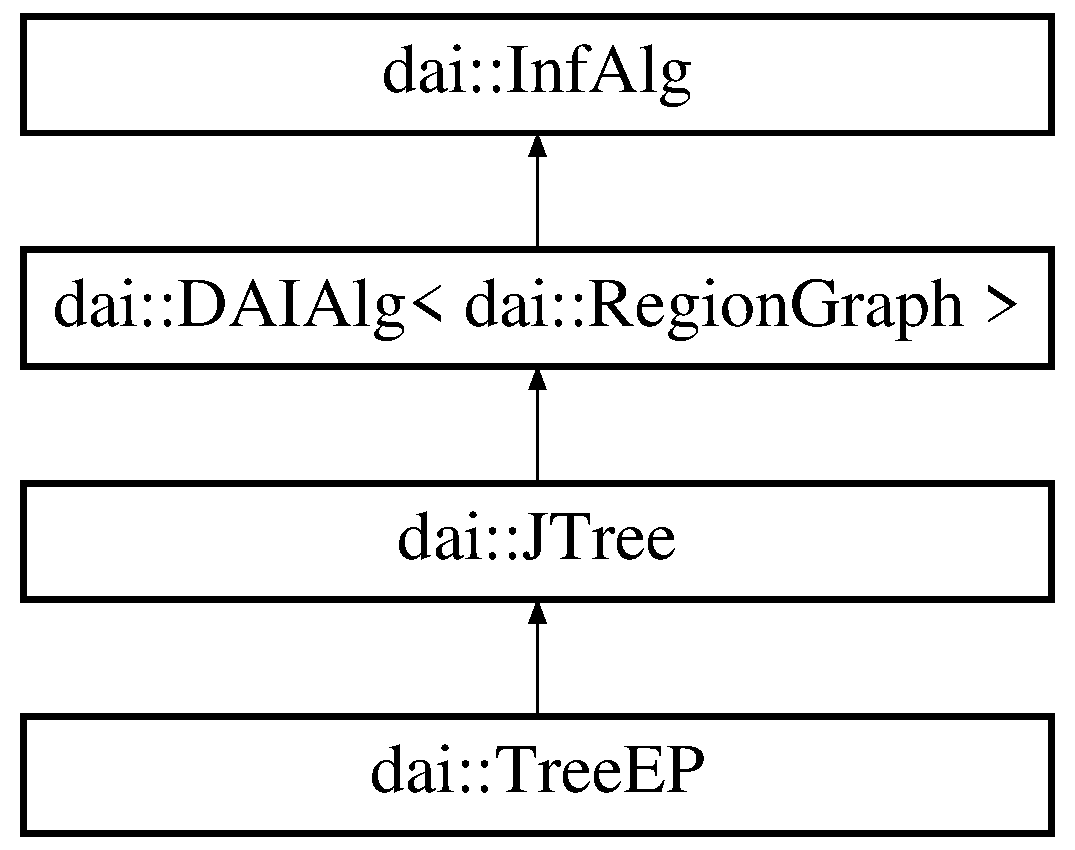
\includegraphics[height=4cm]{classdai_1_1TreeEP}
\end{center}
\end{figure}


\subsection{Detailed Description}
Approximate inference algorithm \char`\"{}TreeEP\char`\"{} by Minka and Qi. \subsection*{Public Member Functions}
\begin{CompactItemize}
\item 
\hypertarget{classdai_1_1TreeEP_5220ad0f0e713305a248963ff65533f8}{
\hyperlink{classdai_1_1TreeEP_5220ad0f0e713305a248963ff65533f8}{TreeEP} ()}
\label{classdai_1_1TreeEP_5220ad0f0e713305a248963ff65533f8}

\begin{CompactList}\small\item\em Default constructor. \item\end{CompactList}\item 
\hypertarget{classdai_1_1TreeEP_a07d388e9201b937cc7275dc9c2d2c8e}{
\hyperlink{classdai_1_1TreeEP_a07d388e9201b937cc7275dc9c2d2c8e}{TreeEP} (const \hyperlink{classdai_1_1TreeEP}{TreeEP} \&x)}
\label{classdai_1_1TreeEP_a07d388e9201b937cc7275dc9c2d2c8e}

\begin{CompactList}\small\item\em Copy constructor. \item\end{CompactList}\item 
\hypertarget{classdai_1_1TreeEP_c3f12eb0685ac91e4f3970accb65b0dd}{
\hyperlink{classdai_1_1TreeEP}{TreeEP} \& \hyperlink{classdai_1_1TreeEP_c3f12eb0685ac91e4f3970accb65b0dd}{operator=} (const \hyperlink{classdai_1_1TreeEP}{TreeEP} \&x)}
\label{classdai_1_1TreeEP_c3f12eb0685ac91e4f3970accb65b0dd}

\begin{CompactList}\small\item\em Assignment operator. \item\end{CompactList}\item 
\hypertarget{classdai_1_1TreeEP_6a1582e1c93f0b9d18fdf08c02201c0f}{
\hyperlink{classdai_1_1TreeEP_6a1582e1c93f0b9d18fdf08c02201c0f}{TreeEP} (const \hyperlink{classdai_1_1FactorGraph}{FactorGraph} \&fg, const \hyperlink{classdai_1_1PropertySet}{PropertySet} \&opts)}
\label{classdai_1_1TreeEP_6a1582e1c93f0b9d18fdf08c02201c0f}

\begin{CompactList}\small\item\em Construct from \hyperlink{classdai_1_1FactorGraph}{FactorGraph} fg and \hyperlink{classdai_1_1PropertySet}{PropertySet} opts. \item\end{CompactList}\item 
\hypertarget{classdai_1_1DAIAlg_48ba6a58d10b8802d690e5e92ec5abe9}{
void \hyperlink{classdai_1_1DAIAlg_48ba6a58d10b8802d690e5e92ec5abe9}{backupFactor} (size\_\-t I)}
\label{classdai_1_1DAIAlg_48ba6a58d10b8802d690e5e92ec5abe9}

\begin{CompactList}\small\item\em Save factor I. \item\end{CompactList}\item 
\hypertarget{classdai_1_1DAIAlg_0176904d3b4b9d083288ea8c4a2dc8bc}{
void \hyperlink{classdai_1_1DAIAlg_0176904d3b4b9d083288ea8c4a2dc8bc}{backupFactors} (const \hyperlink{classdai_1_1VarSet}{VarSet} \&ns)}
\label{classdai_1_1DAIAlg_0176904d3b4b9d083288ea8c4a2dc8bc}

\begin{CompactList}\small\item\em Save Factors involving ns. \item\end{CompactList}\item 
\hypertarget{classdai_1_1DAIAlg_bf8dbd2797ec871e86566a6dfc0864e3}{
void \hyperlink{classdai_1_1DAIAlg_bf8dbd2797ec871e86566a6dfc0864e3}{restoreFactor} (size\_\-t I)}
\label{classdai_1_1DAIAlg_bf8dbd2797ec871e86566a6dfc0864e3}

\begin{CompactList}\small\item\em Restore factor I. \item\end{CompactList}\item 
\hypertarget{classdai_1_1DAIAlg_3ce97e9370f1cdc785526c1a6c1eaadf}{
void \hyperlink{classdai_1_1DAIAlg_3ce97e9370f1cdc785526c1a6c1eaadf}{restoreFactors} (const \hyperlink{classdai_1_1VarSet}{VarSet} \&ns)}
\label{classdai_1_1DAIAlg_3ce97e9370f1cdc785526c1a6c1eaadf}

\begin{CompactList}\small\item\em Restore Factors involving ns. \item\end{CompactList}\item 
\hypertarget{classdai_1_1DAIAlg_b7d537f1a9d116617d8dce722ce65dc0}{
void \hyperlink{classdai_1_1DAIAlg_b7d537f1a9d116617d8dce722ce65dc0}{clamp} (const \hyperlink{classdai_1_1Var}{Var} \&n, size\_\-t i, bool backup=false)}
\label{classdai_1_1DAIAlg_b7d537f1a9d116617d8dce722ce65dc0}

\begin{CompactList}\small\item\em Clamp variable n to value i (i.e. multiply with a Kronecker delta $\delta_{x_n, i}$). \item\end{CompactList}\item 
\hypertarget{classdai_1_1DAIAlg_7f0b8452352080a1e35ab9a68cb589fd}{
void \hyperlink{classdai_1_1DAIAlg_7f0b8452352080a1e35ab9a68cb589fd}{makeCavity} (size\_\-t i, bool backup=false)}
\label{classdai_1_1DAIAlg_7f0b8452352080a1e35ab9a68cb589fd}

\begin{CompactList}\small\item\em Set all factors interacting with var(i) to 1. \item\end{CompactList}\item 
\hypertarget{classdai_1_1DAIAlg_9348542c22d04ed804388f1fe3009fa3}{
\hyperlink{classdai_1_1FactorGraph}{FactorGraph} \& \hyperlink{classdai_1_1DAIAlg_9348542c22d04ed804388f1fe3009fa3}{fg} ()}
\label{classdai_1_1DAIAlg_9348542c22d04ed804388f1fe3009fa3}

\begin{CompactList}\small\item\em Get reference to underlying \hyperlink{classdai_1_1FactorGraph}{FactorGraph}. \item\end{CompactList}\item 
\hypertarget{classdai_1_1DAIAlg_35400e471b8c3c98bef6c74ceac8fa16}{
const \hyperlink{classdai_1_1FactorGraph}{FactorGraph} \& \hyperlink{classdai_1_1DAIAlg_35400e471b8c3c98bef6c74ceac8fa16}{fg} () const }
\label{classdai_1_1DAIAlg_35400e471b8c3c98bef6c74ceac8fa16}

\begin{CompactList}\small\item\em Get const reference to underlying \hyperlink{classdai_1_1FactorGraph}{FactorGraph}. \item\end{CompactList}\end{CompactItemize}
\begin{Indent}{\bf General InfAlg interface}\par
\begin{CompactItemize}
\item 
\hypertarget{classdai_1_1TreeEP_bf27fc154e99ec5a03a95ac50e5898d8}{
virtual \hyperlink{classdai_1_1TreeEP}{TreeEP} $\ast$ \hyperlink{classdai_1_1TreeEP_bf27fc154e99ec5a03a95ac50e5898d8}{clone} () const }
\label{classdai_1_1TreeEP_bf27fc154e99ec5a03a95ac50e5898d8}

\begin{CompactList}\small\item\em Returns a pointer to a new, cloned copy of $\ast$this (i.e., virtual copy constructor). \item\end{CompactList}\item 
\hypertarget{classdai_1_1TreeEP_7edffafcc35bc49aba8d31ad1b16e686}{
virtual \hyperlink{classdai_1_1TreeEP}{TreeEP} $\ast$ \hyperlink{classdai_1_1TreeEP_7edffafcc35bc49aba8d31ad1b16e686}{create} () const }
\label{classdai_1_1TreeEP_7edffafcc35bc49aba8d31ad1b16e686}

\begin{CompactList}\small\item\em Returns a pointer to a newly constructed object $\ast$this (i.e., virtual default constructor). \item\end{CompactList}\item 
\hypertarget{classdai_1_1TreeEP_47053ddaff024856fcb870ce38d99370}{
virtual std::string \hyperlink{classdai_1_1TreeEP_47053ddaff024856fcb870ce38d99370}{identify} () const }
\label{classdai_1_1TreeEP_47053ddaff024856fcb870ce38d99370}

\begin{CompactList}\small\item\em Identifies itself for logging purposes. \item\end{CompactList}\item 
\hypertarget{classdai_1_1TreeEP_c02c63b00dc84333b7cc1fa5b1c45667}{
virtual \hyperlink{namespacedai_e7d0472fdc89a8635825d01940e91cbf}{Real} \hyperlink{classdai_1_1TreeEP_c02c63b00dc84333b7cc1fa5b1c45667}{logZ} () const }
\label{classdai_1_1TreeEP_c02c63b00dc84333b7cc1fa5b1c45667}

\begin{CompactList}\small\item\em Returns the logarithm of the (approximated) partition sum (normalizing constant of the factor graph). \item\end{CompactList}\item 
virtual void \hyperlink{classdai_1_1TreeEP_fff5580fa87ce391223a2e2867527248}{init} ()
\begin{CompactList}\small\item\em Initializes all data structures of the approximate inference algorithm. \item\end{CompactList}\item 
virtual void \hyperlink{classdai_1_1TreeEP_3cc3718d1fbdf67db23a846283f99d08}{init} (const \hyperlink{classdai_1_1VarSet}{VarSet} \&)
\begin{CompactList}\small\item\em Initializes all data structures corresponding to some set of variables. \item\end{CompactList}\item 
\hypertarget{classdai_1_1TreeEP_aecaf7e050a913c082a2ce5b9f97d744}{
virtual double \hyperlink{classdai_1_1TreeEP_aecaf7e050a913c082a2ce5b9f97d744}{run} ()}
\label{classdai_1_1TreeEP_aecaf7e050a913c082a2ce5b9f97d744}

\begin{CompactList}\small\item\em Runs the approximate inference algorithm. \item\end{CompactList}\item 
virtual double \hyperlink{classdai_1_1TreeEP_d1214cd7bc0899d1a8dc4523bacdb488}{maxDiff} () const 
\item 
virtual size\_\-t \hyperlink{classdai_1_1TreeEP_e18e681d1f078e42445d39f8605df7d4}{Iterations} () const 
\end{CompactItemize}
\end{Indent}
\begin{Indent}{\bf General InfAlg interface}\par
\begin{CompactItemize}
\item 
\hypertarget{classdai_1_1JTree_432cdc9cc9f4be26509e6bd2337c5325}{
virtual \hyperlink{classdai_1_1TFactor}{Factor} \hyperlink{classdai_1_1JTree_432cdc9cc9f4be26509e6bd2337c5325}{belief} (const \hyperlink{classdai_1_1Var}{Var} \&n) const }
\label{classdai_1_1JTree_432cdc9cc9f4be26509e6bd2337c5325}

\begin{CompactList}\small\item\em Returns the \char`\"{}belief\char`\"{} (i.e., approximate marginal probability distribution) of a variable. \item\end{CompactList}\item 
\hypertarget{classdai_1_1JTree_10de7513fea42d8c02be95a30bb69553}{
virtual \hyperlink{classdai_1_1TFactor}{Factor} \hyperlink{classdai_1_1JTree_10de7513fea42d8c02be95a30bb69553}{belief} (const \hyperlink{classdai_1_1VarSet}{VarSet} \&ns) const }
\label{classdai_1_1JTree_10de7513fea42d8c02be95a30bb69553}

\begin{CompactList}\small\item\em Returns the \char`\"{}belief\char`\"{} (i.e., approximate marginal probability distribution) of a set of variables. \item\end{CompactList}\item 
\hypertarget{classdai_1_1JTree_3c16a15fe017649fec4d63455fda6843}{
virtual std::vector$<$ \hyperlink{classdai_1_1TFactor}{Factor} $>$ \hyperlink{classdai_1_1JTree_3c16a15fe017649fec4d63455fda6843}{beliefs} () const }
\label{classdai_1_1JTree_3c16a15fe017649fec4d63455fda6843}

\begin{CompactList}\small\item\em Returns all \char`\"{}beliefs\char`\"{} (i.e., approximate marginal probability distribution) calculated by the algorithm. \item\end{CompactList}\end{CompactItemize}
\end{Indent}
\begin{Indent}{\bf Additional interface specific for JTree}\par
\begin{CompactItemize}
\item 
\hypertarget{classdai_1_1JTree_0898a401baee9af694f636d174048a46}{
void \textbf{GenerateJT} (const std::vector$<$ \hyperlink{classdai_1_1VarSet}{VarSet} $>$ \&Cliques)}
\label{classdai_1_1JTree_0898a401baee9af694f636d174048a46}

\item 
\hypertarget{classdai_1_1JTree_5a96942bd16a4e4e10fcf720c1b0e04b}{
\hyperlink{classdai_1_1TFactor}{Factor} \& \hyperlink{classdai_1_1JTree_5a96942bd16a4e4e10fcf720c1b0e04b}{message} (size\_\-t alpha, size\_\-t \_\-beta)}
\label{classdai_1_1JTree_5a96942bd16a4e4e10fcf720c1b0e04b}

\begin{CompactList}\small\item\em Returns reference the message from outer region alpha to its \_\-beta'th neighboring inner region. \item\end{CompactList}\item 
\hypertarget{classdai_1_1JTree_e59c0012cbd6a425704fd637f9fed4c5}{
const \hyperlink{classdai_1_1TFactor}{Factor} \& \hyperlink{classdai_1_1JTree_e59c0012cbd6a425704fd637f9fed4c5}{message} (size\_\-t alpha, size\_\-t \_\-beta) const }
\label{classdai_1_1JTree_e59c0012cbd6a425704fd637f9fed4c5}

\begin{CompactList}\small\item\em Returns const reference to the message from outer region alpha to its \_\-beta'th neighboring inner region. \item\end{CompactList}\item 
\hypertarget{classdai_1_1JTree_4569d21624cb49d9a79c3c8332e0d4b3}{
void \hyperlink{classdai_1_1JTree_4569d21624cb49d9a79c3c8332e0d4b3}{runHUGIN} ()}
\label{classdai_1_1JTree_4569d21624cb49d9a79c3c8332e0d4b3}

\begin{CompactList}\small\item\em Runs junction-tree with HUGIN updates. \item\end{CompactList}\item 
\hypertarget{classdai_1_1JTree_6d8ee4f30498985d0d434988dba8c258}{
void \hyperlink{classdai_1_1JTree_6d8ee4f30498985d0d434988dba8c258}{runShaferShenoy} ()}
\label{classdai_1_1JTree_6d8ee4f30498985d0d434988dba8c258}

\begin{CompactList}\small\item\em Runs junction-tree with Shafer-Shenoy updates. \item\end{CompactList}\item 
\hypertarget{classdai_1_1JTree_0ee81ed10535369928ba0abb3c1f7e02}{
size\_\-t \hyperlink{classdai_1_1JTree_0ee81ed10535369928ba0abb3c1f7e02}{findEfficientTree} (const \hyperlink{classdai_1_1VarSet}{VarSet} \&ns, \hyperlink{namespacedai_e7764251ab4d4b2d4fbec214eac83079}{DEdgeVec} \&Tree, size\_\-t PreviousRoot=(size\_\-t)-1) const }
\label{classdai_1_1JTree_0ee81ed10535369928ba0abb3c1f7e02}

\begin{CompactList}\small\item\em Finds an efficient tree for calculating the marginal of some variables. \item\end{CompactList}\item 
\hypertarget{classdai_1_1JTree_2ffd2a47a85b81efbbb5f0cfd7a083fa}{
\hyperlink{classdai_1_1TFactor}{Factor} \hyperlink{classdai_1_1JTree_2ffd2a47a85b81efbbb5f0cfd7a083fa}{calcMarginal} (const \hyperlink{classdai_1_1VarSet}{VarSet} \&ns)}
\label{classdai_1_1JTree_2ffd2a47a85b81efbbb5f0cfd7a083fa}

\begin{CompactList}\small\item\em Calculates the marginal of a set of variables. \item\end{CompactList}\end{CompactItemize}
\end{Indent}
\subsection*{Public Attributes}
\begin{CompactItemize}
\item 
\hypertarget{classdai_1_1TreeEP_b81687eb1c926bb9cbfc62de14bad58b}{
struct \hyperlink{structdai_1_1TreeEP_1_1Properties}{dai::TreeEP::Properties} \hyperlink{classdai_1_1TreeEP_b81687eb1c926bb9cbfc62de14bad58b}{props}}
\label{classdai_1_1TreeEP_b81687eb1c926bb9cbfc62de14bad58b}

\begin{CompactList}\small\item\em Parameters of this inference algorithm. \item\end{CompactList}\item 
\hypertarget{classdai_1_1JTree_6ddedae95e2dda19e20b7b49455ea389}{
\hyperlink{namespacedai_e7764251ab4d4b2d4fbec214eac83079}{DEdgeVec} \hyperlink{classdai_1_1JTree_6ddedae95e2dda19e20b7b49455ea389}{RTree}}
\label{classdai_1_1JTree_6ddedae95e2dda19e20b7b49455ea389}

\begin{CompactList}\small\item\em Rooted tree. \item\end{CompactList}\item 
\hypertarget{classdai_1_1JTree_66cdd4d8258582aaf794466f3786dbfb}{
std::vector$<$ \hyperlink{classdai_1_1TFactor}{Factor} $>$ \hyperlink{classdai_1_1JTree_66cdd4d8258582aaf794466f3786dbfb}{Qa}}
\label{classdai_1_1JTree_66cdd4d8258582aaf794466f3786dbfb}

\begin{CompactList}\small\item\em Outer region beliefs. \item\end{CompactList}\item 
\hypertarget{classdai_1_1JTree_9d93e9f387d9772be5bc2b5372f7d20d}{
std::vector$<$ \hyperlink{classdai_1_1TFactor}{Factor} $>$ \hyperlink{classdai_1_1JTree_9d93e9f387d9772be5bc2b5372f7d20d}{Qb}}
\label{classdai_1_1JTree_9d93e9f387d9772be5bc2b5372f7d20d}

\begin{CompactList}\small\item\em Inner region beliefs. \item\end{CompactList}\end{CompactItemize}
\subsection*{Static Public Attributes}
\begin{CompactItemize}
\item 
\hypertarget{classdai_1_1TreeEP_28af8be0b7d337c266286118351059f9}{
static const char $\ast$ \hyperlink{classdai_1_1TreeEP_28af8be0b7d337c266286118351059f9}{Name} = \char`\"{}TREEEP\char`\"{}}
\label{classdai_1_1TreeEP_28af8be0b7d337c266286118351059f9}

\begin{CompactList}\small\item\em Name of this inference method. \item\end{CompactList}\end{CompactItemize}
\subsection*{Related Functions}
(Note that these are not member functions.) \begin{CompactItemize}
\item 
std::pair$<$ size\_\-t, size\_\-t $>$ \hyperlink{classdai_1_1JTree_bca2633ffb8701cb62c54241bdad307e}{treewidth} (const \hyperlink{classdai_1_1FactorGraph}{FactorGraph} \&fg)
\begin{CompactList}\small\item\em Calculates upper bound to the treewidth of a \hyperlink{classdai_1_1FactorGraph}{FactorGraph}. \item\end{CompactList}\end{CompactItemize}
\subsection*{Classes}
\begin{CompactItemize}
\item 
struct \hyperlink{structdai_1_1TreeEP_1_1Properties}{Properties}
\begin{CompactList}\small\item\em Parameters of this inference algorithm. \item\end{CompactList}\item 
class \textbf{TreeEPSubTree}
\end{CompactItemize}


\subsection{Member Function Documentation}
\hypertarget{classdai_1_1TreeEP_fff5580fa87ce391223a2e2867527248}{
\index{dai::TreeEP@{dai::TreeEP}!init@{init}}
\index{init@{init}!dai::TreeEP@{dai::TreeEP}}
\subsubsection[init]{\setlength{\rightskip}{0pt plus 5cm}void dai::TreeEP::init ()\hspace{0.3cm}{\tt  \mbox{[}virtual\mbox{]}}}}
\label{classdai_1_1TreeEP_fff5580fa87ce391223a2e2867527248}


Initializes all data structures of the approximate inference algorithm. 

This method should be called at least once before \hyperlink{classdai_1_1TreeEP_aecaf7e050a913c082a2ce5b9f97d744}{run()} is called 

Reimplemented from \hyperlink{classdai_1_1JTree_cbb2df1dc4e64097a46fc4cb1394e76f}{dai::JTree}.\hypertarget{classdai_1_1TreeEP_3cc3718d1fbdf67db23a846283f99d08}{
\index{dai::TreeEP@{dai::TreeEP}!init@{init}}
\index{init@{init}!dai::TreeEP@{dai::TreeEP}}
\subsubsection[init]{\setlength{\rightskip}{0pt plus 5cm}virtual void dai::TreeEP::init (const {\bf VarSet} \& {\em ns})\hspace{0.3cm}{\tt  \mbox{[}inline, virtual\mbox{]}}}}
\label{classdai_1_1TreeEP_3cc3718d1fbdf67db23a846283f99d08}


Initializes all data structures corresponding to some set of variables. 

This method can be used to do a partial initialization after a part of the factor graph has changed. Instead of initializing all data structures, it only initializes those involving the variables in ns. 

Reimplemented from \hyperlink{classdai_1_1JTree_365c52b5f264c844ac5c010026719350}{dai::JTree}.\hypertarget{classdai_1_1TreeEP_d1214cd7bc0899d1a8dc4523bacdb488}{
\index{dai::TreeEP@{dai::TreeEP}!maxDiff@{maxDiff}}
\index{maxDiff@{maxDiff}!dai::TreeEP@{dai::TreeEP}}
\subsubsection[maxDiff]{\setlength{\rightskip}{0pt plus 5cm}virtual double dai::TreeEP::maxDiff () const\hspace{0.3cm}{\tt  \mbox{[}inline, virtual\mbox{]}}}}
\label{classdai_1_1TreeEP_d1214cd7bc0899d1a8dc4523bacdb488}


Return maximum difference between single node beliefs in the last pass \begin{Desc}
\item[Exceptions:]
\begin{description}
\item[{\em \hyperlink{classdai_1_1Exception}{Exception}}]if not implemented/supported \end{description}
\end{Desc}


Reimplemented from \hyperlink{classdai_1_1JTree_acd3916835c9d349aa1b22a2dd54de83}{dai::JTree}.\hypertarget{classdai_1_1TreeEP_e18e681d1f078e42445d39f8605df7d4}{
\index{dai::TreeEP@{dai::TreeEP}!Iterations@{Iterations}}
\index{Iterations@{Iterations}!dai::TreeEP@{dai::TreeEP}}
\subsubsection[Iterations]{\setlength{\rightskip}{0pt plus 5cm}virtual size\_\-t dai::TreeEP::Iterations () const\hspace{0.3cm}{\tt  \mbox{[}inline, virtual\mbox{]}}}}
\label{classdai_1_1TreeEP_e18e681d1f078e42445d39f8605df7d4}


Return number of passes over the factorgraph \begin{Desc}
\item[Exceptions:]
\begin{description}
\item[{\em \hyperlink{classdai_1_1Exception}{Exception}}]if not implemented/supported \end{description}
\end{Desc}


Reimplemented from \hyperlink{classdai_1_1JTree_71cd98f072d69f6ce60af8b52ef02eb8}{dai::JTree}.

\subsection{Friends And Related Function Documentation}
\hypertarget{classdai_1_1JTree_bca2633ffb8701cb62c54241bdad307e}{
\index{dai::TreeEP@{dai::TreeEP}!treewidth@{treewidth}}
\index{treewidth@{treewidth}!dai::TreeEP@{dai::TreeEP}}
\subsubsection[treewidth]{\setlength{\rightskip}{0pt plus 5cm}std::pair$<$ size\_\-t, size\_\-t $>$ treewidth (const {\bf FactorGraph} \& {\em fg})\hspace{0.3cm}{\tt  \mbox{[}related, inherited\mbox{]}}}}
\label{classdai_1_1JTree_bca2633ffb8701cb62c54241bdad307e}


Calculates upper bound to the treewidth of a \hyperlink{classdai_1_1FactorGraph}{FactorGraph}. 

\begin{Desc}
\item[Returns:]a pair (number of variables in largest clique, number of states in largest clique) \end{Desc}


The documentation for this class was generated from the following files:\begin{CompactItemize}
\item 
include/dai/\hyperlink{treeep_8h}{treeep.h}\item 
src/treeep.cpp\end{CompactItemize}

\hypertarget{structdai_1_1TreeEP_1_1Properties}{
\section{dai::TreeEP::Properties Struct Reference}
\label{structdai_1_1TreeEP_1_1Properties}\index{dai::TreeEP::Properties@{dai::TreeEP::Properties}}
}
{\tt \#include $<$dai/treeep.h$>$}



\subsection{Detailed Description}
Parameters of this inference algorithm. \subsection*{Public Attributes}
\begin{CompactItemize}
\item 
size\_\-t \hyperlink{structdai_1_1TreeEP_1_1Properties_f41d83b6886eed09e080420be1fe0486}{verbose}
\begin{CompactList}\small\item\em Enumeration of possible choices for the tree. \item\end{CompactList}\item 
\hypertarget{structdai_1_1TreeEP_1_1Properties_58b7b2658dfa173a64a1683a6ac5425d}{
size\_\-t \hyperlink{structdai_1_1TreeEP_1_1Properties_58b7b2658dfa173a64a1683a6ac5425d}{maxiter}}
\label{structdai_1_1TreeEP_1_1Properties_58b7b2658dfa173a64a1683a6ac5425d}

\begin{CompactList}\small\item\em Maximum number of iterations. \item\end{CompactList}\item 
\hypertarget{structdai_1_1TreeEP_1_1Properties_084e74547be3ae87576ce6ee849fea5f}{
double \hyperlink{structdai_1_1TreeEP_1_1Properties_084e74547be3ae87576ce6ee849fea5f}{tol}}
\label{structdai_1_1TreeEP_1_1Properties_084e74547be3ae87576ce6ee849fea5f}

\begin{CompactList}\small\item\em Tolerance. \item\end{CompactList}\item 
\hypertarget{structdai_1_1TreeEP_1_1Properties_f80877d6d20176db4bc8367b6185e2d3}{
TypeType \hyperlink{structdai_1_1TreeEP_1_1Properties_f80877d6d20176db4bc8367b6185e2d3}{type}}
\label{structdai_1_1TreeEP_1_1Properties_f80877d6d20176db4bc8367b6185e2d3}

\begin{CompactList}\small\item\em How to choose the tree. \item\end{CompactList}\end{CompactItemize}


\subsection{Member Data Documentation}
\hypertarget{structdai_1_1TreeEP_1_1Properties_f41d83b6886eed09e080420be1fe0486}{
\index{dai::TreeEP::Properties@{dai::TreeEP::Properties}!verbose@{verbose}}
\index{verbose@{verbose}!dai::TreeEP::Properties@{dai::TreeEP::Properties}}
\subsubsection[verbose]{\setlength{\rightskip}{0pt plus 5cm}size\_\-t {\bf dai::TreeEP::Properties::verbose}}}
\label{structdai_1_1TreeEP_1_1Properties_f41d83b6886eed09e080420be1fe0486}


Enumeration of possible choices for the tree. 

Verbosity 

The documentation for this struct was generated from the following file:\begin{CompactItemize}
\item 
include/dai/\hyperlink{treeep_8h}{treeep.h}\end{CompactItemize}

\hypertarget{classdai_1_1UEdge}{
\section{dai::UEdge Class Reference}
\label{classdai_1_1UEdge}\index{dai::UEdge@{dai::UEdge}}
}
{\tt \#include $<$dai/weightedgraph.h$>$}



\subsection{Detailed Description}
Undirected edge between nodes n1 and n2. \subsection*{Public Member Functions}
\begin{CompactItemize}
\item 
\hypertarget{classdai_1_1UEdge_42ec52c9396a94aafd7fd62a9b36067e}{
\hyperlink{classdai_1_1UEdge_42ec52c9396a94aafd7fd62a9b36067e}{UEdge} ()}
\label{classdai_1_1UEdge_42ec52c9396a94aafd7fd62a9b36067e}

\begin{CompactList}\small\item\em Default constructor. \item\end{CompactList}\item 
\hypertarget{classdai_1_1UEdge_1e7819b6b776d0715207b251a8c951fe}{
\hyperlink{classdai_1_1UEdge_1e7819b6b776d0715207b251a8c951fe}{UEdge} (size\_\-t m1, size\_\-t m2)}
\label{classdai_1_1UEdge_1e7819b6b776d0715207b251a8c951fe}

\begin{CompactList}\small\item\em Constructor. \item\end{CompactList}\item 
\hypertarget{classdai_1_1UEdge_31d68730f49619179aff649cbe5c3d3d}{
\hyperlink{classdai_1_1UEdge_31d68730f49619179aff649cbe5c3d3d}{UEdge} (const \hyperlink{classdai_1_1DEdge}{DEdge} \&e)}
\label{classdai_1_1UEdge_31d68730f49619179aff649cbe5c3d3d}

\begin{CompactList}\small\item\em Construct from \hyperlink{classdai_1_1DEdge}{DEdge}. \item\end{CompactList}\item 
\hypertarget{classdai_1_1UEdge_6104711a37099d2bea16ebc26f35592d}{
bool \hyperlink{classdai_1_1UEdge_6104711a37099d2bea16ebc26f35592d}{operator==} (const \hyperlink{classdai_1_1UEdge}{UEdge} \&x)}
\label{classdai_1_1UEdge_6104711a37099d2bea16ebc26f35592d}

\begin{CompactList}\small\item\em Tests for inequality (disregarding the ordering of n1 and n2). \item\end{CompactList}\item 
\hypertarget{classdai_1_1UEdge_c18760d5642f14aa1b64e0d3c611cb0f}{
bool \hyperlink{classdai_1_1UEdge_c18760d5642f14aa1b64e0d3c611cb0f}{operator$<$} (const \hyperlink{classdai_1_1UEdge}{UEdge} \&x) const }
\label{classdai_1_1UEdge_c18760d5642f14aa1b64e0d3c611cb0f}

\begin{CompactList}\small\item\em Smaller-than operator. \item\end{CompactList}\end{CompactItemize}
\subsection*{Public Attributes}
\begin{CompactItemize}
\item 
\hypertarget{classdai_1_1UEdge_d977fc954195ab7913c57d50639da25c}{
size\_\-t \hyperlink{classdai_1_1UEdge_d977fc954195ab7913c57d50639da25c}{n1}}
\label{classdai_1_1UEdge_d977fc954195ab7913c57d50639da25c}

\begin{CompactList}\small\item\em First node index. \item\end{CompactList}\item 
\hypertarget{classdai_1_1UEdge_f2c3cb4413b81fe69fcc4cbedbd17723}{
size\_\-t \hyperlink{classdai_1_1UEdge_f2c3cb4413b81fe69fcc4cbedbd17723}{n2}}
\label{classdai_1_1UEdge_f2c3cb4413b81fe69fcc4cbedbd17723}

\begin{CompactList}\small\item\em Second node index. \item\end{CompactList}\end{CompactItemize}
\subsection*{Friends}
\begin{CompactItemize}
\item 
\hypertarget{classdai_1_1UEdge_d723be19b6d346867d5477ae26cc4bf1}{
std::ostream \& \hyperlink{classdai_1_1UEdge_d723be19b6d346867d5477ae26cc4bf1}{operator$<$$<$} (std::ostream \&os, const \hyperlink{classdai_1_1UEdge}{UEdge} \&e)}
\label{classdai_1_1UEdge_d723be19b6d346867d5477ae26cc4bf1}

\begin{CompactList}\small\item\em Writes a \hyperlink{classdai_1_1UEdge}{UEdge} to an output stream. \item\end{CompactList}\end{CompactItemize}


The documentation for this class was generated from the following file:\begin{CompactItemize}
\item 
include/dai/\hyperlink{weightedgraph_8h}{weightedgraph.h}\end{CompactItemize}

\hypertarget{classdai_1_1Var}{
\section{dai::Var Class Reference}
\label{classdai_1_1Var}\index{dai::Var@{dai::Var}}
}
{\tt \#include $<$dai/var.h$>$}



\subsection{Detailed Description}
Represents a discrete random variable. 

It contains the {\em label\/} of the variable (an integer-valued unique ID) and the number of possible values ({\em states\/}) of the variable. \subsection*{Public Member Functions}
\begin{CompactItemize}
\item 
\hypertarget{classdai_1_1Var_f8261d1878d0930ad9914f2a9fa2ef40}{
\hyperlink{classdai_1_1Var_f8261d1878d0930ad9914f2a9fa2ef40}{Var} ()}
\label{classdai_1_1Var_f8261d1878d0930ad9914f2a9fa2ef40}

\begin{CompactList}\small\item\em Default constructor. \item\end{CompactList}\item 
\hypertarget{classdai_1_1Var_38eeca70cd2dbb8bc793c406af79a5b8}{
\hyperlink{classdai_1_1Var_38eeca70cd2dbb8bc793c406af79a5b8}{Var} (long label, size\_\-t states)}
\label{classdai_1_1Var_38eeca70cd2dbb8bc793c406af79a5b8}

\begin{CompactList}\small\item\em Constructor. \item\end{CompactList}\item 
\hypertarget{classdai_1_1Var_1570f11c8b5acdacd5234b9897ae6914}{
long \hyperlink{classdai_1_1Var_1570f11c8b5acdacd5234b9897ae6914}{label} () const }
\label{classdai_1_1Var_1570f11c8b5acdacd5234b9897ae6914}

\begin{CompactList}\small\item\em Returns the label. \item\end{CompactList}\item 
\hypertarget{classdai_1_1Var_f71c9cda72e600e7fb8b41fe15bd2054}{
long \& \hyperlink{classdai_1_1Var_f71c9cda72e600e7fb8b41fe15bd2054}{label} ()}
\label{classdai_1_1Var_f71c9cda72e600e7fb8b41fe15bd2054}

\begin{CompactList}\small\item\em Returns reference to label. \item\end{CompactList}\item 
\hypertarget{classdai_1_1Var_41f8d939741336bca2080bedfaf92302}{
size\_\-t \hyperlink{classdai_1_1Var_41f8d939741336bca2080bedfaf92302}{states} () const }
\label{classdai_1_1Var_41f8d939741336bca2080bedfaf92302}

\begin{CompactList}\small\item\em Returns the number of states. \item\end{CompactList}\item 
\hypertarget{classdai_1_1Var_274936b287bddd1b6384b52907df7e31}{
size\_\-t \& \hyperlink{classdai_1_1Var_274936b287bddd1b6384b52907df7e31}{states} ()}
\label{classdai_1_1Var_274936b287bddd1b6384b52907df7e31}

\begin{CompactList}\small\item\em Returns reference to number of states. \item\end{CompactList}\item 
\hypertarget{classdai_1_1Var_c997b317a3b324312d03d8adaf387f15}{
bool \hyperlink{classdai_1_1Var_c997b317a3b324312d03d8adaf387f15}{operator$<$} (const \hyperlink{classdai_1_1Var}{Var} \&n) const }
\label{classdai_1_1Var_c997b317a3b324312d03d8adaf387f15}

\begin{CompactList}\small\item\em Smaller-than operator (only compares labels). \item\end{CompactList}\item 
\hypertarget{classdai_1_1Var_d7480992a3c33f1b18e7b18b1f7f4241}{
bool \hyperlink{classdai_1_1Var_d7480992a3c33f1b18e7b18b1f7f4241}{operator$>$} (const \hyperlink{classdai_1_1Var}{Var} \&n) const }
\label{classdai_1_1Var_d7480992a3c33f1b18e7b18b1f7f4241}

\begin{CompactList}\small\item\em Larger-than operator (only compares labels). \item\end{CompactList}\item 
\hypertarget{classdai_1_1Var_deaba07976118ad2b6b2d891a4bf2009}{
bool \hyperlink{classdai_1_1Var_deaba07976118ad2b6b2d891a4bf2009}{operator$<$=} (const \hyperlink{classdai_1_1Var}{Var} \&n) const }
\label{classdai_1_1Var_deaba07976118ad2b6b2d891a4bf2009}

\begin{CompactList}\small\item\em Smaller-than-or-equal-to operator (only compares labels). \item\end{CompactList}\item 
\hypertarget{classdai_1_1Var_7bfc52374ce25ebf05f9bd8387512428}{
bool \hyperlink{classdai_1_1Var_7bfc52374ce25ebf05f9bd8387512428}{operator$>$=} (const \hyperlink{classdai_1_1Var}{Var} \&n) const }
\label{classdai_1_1Var_7bfc52374ce25ebf05f9bd8387512428}

\begin{CompactList}\small\item\em Larger-than-or-equal-to operator (only compares labels). \item\end{CompactList}\item 
\hypertarget{classdai_1_1Var_b0668fe05276356dd72bc0c4ba8e38fb}{
bool \hyperlink{classdai_1_1Var_b0668fe05276356dd72bc0c4ba8e38fb}{operator!=} (const \hyperlink{classdai_1_1Var}{Var} \&n) const }
\label{classdai_1_1Var_b0668fe05276356dd72bc0c4ba8e38fb}

\begin{CompactList}\small\item\em Not-equal-to operator (only compares labels). \item\end{CompactList}\item 
\hypertarget{classdai_1_1Var_6c82ecf70996c18280e063d1c5e02834}{
bool \hyperlink{classdai_1_1Var_6c82ecf70996c18280e063d1c5e02834}{operator==} (const \hyperlink{classdai_1_1Var}{Var} \&n) const }
\label{classdai_1_1Var_6c82ecf70996c18280e063d1c5e02834}

\begin{CompactList}\small\item\em Equal-to operator (only compares labels). \item\end{CompactList}\end{CompactItemize}
\subsection*{Friends}
\begin{CompactItemize}
\item 
\hypertarget{classdai_1_1Var_2afe0ebb307f835920656e75f9a1961e}{
std::ostream \& \hyperlink{classdai_1_1Var_2afe0ebb307f835920656e75f9a1961e}{operator$<$$<$} (std::ostream \&os, const \hyperlink{classdai_1_1Var}{Var} \&n)}
\label{classdai_1_1Var_2afe0ebb307f835920656e75f9a1961e}

\begin{CompactList}\small\item\em Writes a \hyperlink{classdai_1_1Var}{Var} to an output stream. \item\end{CompactList}\end{CompactItemize}


The documentation for this class was generated from the following file:\begin{CompactItemize}
\item 
include/dai/\hyperlink{var_8h}{var.h}\end{CompactItemize}

\hypertarget{classdai_1_1VarSet}{
\section{dai::VarSet Class Reference}
\label{classdai_1_1VarSet}\index{dai::VarSet@{dai::VarSet}}
}
{\tt \#include $<$dai/varset.h$>$}

Inheritance diagram for dai::VarSet::\begin{figure}[H]
\begin{center}
\leavevmode
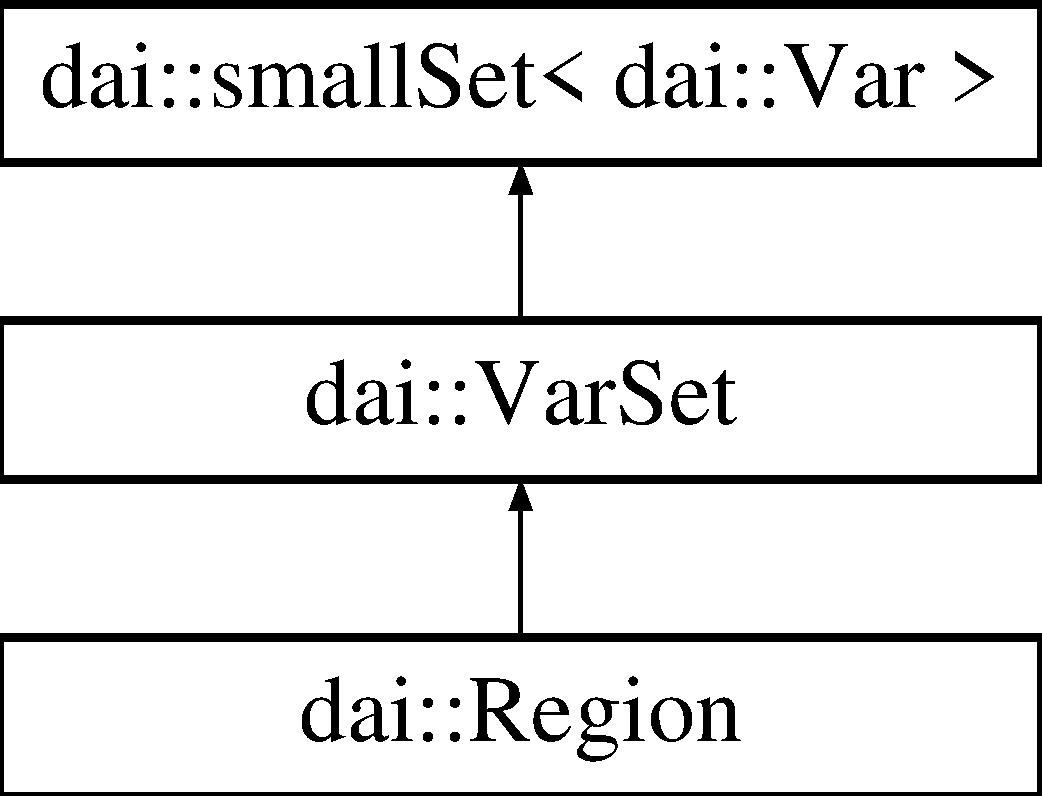
\includegraphics[height=3cm]{classdai_1_1VarSet}
\end{center}
\end{figure}


\subsection{Detailed Description}
Represents a set of variables. 

\begin{Desc}
\item[Note:]A \hyperlink{classdai_1_1VarSet}{VarSet} is implemented using a std::vector$<$Var$>$ instead of the more natural std::set$<$Var$>$ because of efficiency reasons. \end{Desc}
\subsection*{Public Types}
\begin{CompactItemize}
\item 
\hypertarget{classdai_1_1smallSet_103c819872818d14a7234a1f618a815c}{
typedef std::vector$<$ T $>$::\hyperlink{classdai_1_1smallSet_103c819872818d14a7234a1f618a815c}{const\_\-iterator} \hyperlink{classdai_1_1smallSet_103c819872818d14a7234a1f618a815c}{const\_\-iterator}}
\label{classdai_1_1smallSet_103c819872818d14a7234a1f618a815c}

\begin{CompactList}\small\item\em Constant iterator over the elements. \item\end{CompactList}\item 
\hypertarget{classdai_1_1smallSet_254dd4f8cad9c7bce5522e9dbcfc4f49}{
typedef std::vector$<$ T $>$::\hyperlink{classdai_1_1smallSet_254dd4f8cad9c7bce5522e9dbcfc4f49}{iterator} \hyperlink{classdai_1_1smallSet_254dd4f8cad9c7bce5522e9dbcfc4f49}{iterator}}
\label{classdai_1_1smallSet_254dd4f8cad9c7bce5522e9dbcfc4f49}

\begin{CompactList}\small\item\em Iterator over the elements. \item\end{CompactList}\item 
\hypertarget{classdai_1_1smallSet_46882a9010267d41f447feb6aaf65cc1}{
typedef std::vector$<$ T $>$::\hyperlink{classdai_1_1smallSet_46882a9010267d41f447feb6aaf65cc1}{const\_\-reverse\_\-iterator} \hyperlink{classdai_1_1smallSet_46882a9010267d41f447feb6aaf65cc1}{const\_\-reverse\_\-iterator}}
\label{classdai_1_1smallSet_46882a9010267d41f447feb6aaf65cc1}

\begin{CompactList}\small\item\em Constant reverse iterator over the elements. \item\end{CompactList}\item 
\hypertarget{classdai_1_1smallSet_6dea3ee0aa40c4312e6278a7d17f516d}{
typedef std::vector$<$ T $>$::\hyperlink{classdai_1_1smallSet_6dea3ee0aa40c4312e6278a7d17f516d}{reverse\_\-iterator} \hyperlink{classdai_1_1smallSet_6dea3ee0aa40c4312e6278a7d17f516d}{reverse\_\-iterator}}
\label{classdai_1_1smallSet_6dea3ee0aa40c4312e6278a7d17f516d}

\begin{CompactList}\small\item\em Reverse iterator over the elements. \item\end{CompactList}\end{CompactItemize}
\subsection*{Public Member Functions}
\begin{CompactItemize}
\item 
\hypertarget{classdai_1_1VarSet_933a982d2d7f8c2f796610ab351d728b}{
\hyperlink{classdai_1_1VarSet_933a982d2d7f8c2f796610ab351d728b}{VarSet} ()}
\label{classdai_1_1VarSet_933a982d2d7f8c2f796610ab351d728b}

\begin{CompactList}\small\item\em Default constructor. \item\end{CompactList}\item 
\hypertarget{classdai_1_1VarSet_547ebf0ada78ea9baa2ad3f0c6225206}{
\hyperlink{classdai_1_1VarSet_547ebf0ada78ea9baa2ad3f0c6225206}{VarSet} (const \hyperlink{classdai_1_1VarSet}{VarSet} \&x)}
\label{classdai_1_1VarSet_547ebf0ada78ea9baa2ad3f0c6225206}

\begin{CompactList}\small\item\em Copy constructor. \item\end{CompactList}\item 
\hypertarget{classdai_1_1VarSet_3a551f98ea573b932042d393e5414c15}{
\hyperlink{classdai_1_1VarSet}{VarSet} \& \hyperlink{classdai_1_1VarSet_3a551f98ea573b932042d393e5414c15}{operator=} (const \hyperlink{classdai_1_1VarSet}{VarSet} \&x)}
\label{classdai_1_1VarSet_3a551f98ea573b932042d393e5414c15}

\begin{CompactList}\small\item\em Assignment operator. \item\end{CompactList}\item 
\hypertarget{classdai_1_1VarSet_c15195c92c88c8f9f477dafab47937af}{
\hyperlink{classdai_1_1VarSet_c15195c92c88c8f9f477dafab47937af}{VarSet} (const \hyperlink{classdai_1_1smallSet}{smallSet}$<$ \hyperlink{classdai_1_1Var}{Var} $>$ \&x)}
\label{classdai_1_1VarSet_c15195c92c88c8f9f477dafab47937af}

\begin{CompactList}\small\item\em Construct from smallSet$<$Var$>$. \item\end{CompactList}\item 
\hypertarget{classdai_1_1VarSet_adfd4d43a9a521f8738e9507682440d3}{
size\_\-t \hyperlink{classdai_1_1VarSet_adfd4d43a9a521f8738e9507682440d3}{nrStates} ()}
\label{classdai_1_1VarSet_adfd4d43a9a521f8738e9507682440d3}

\begin{CompactList}\small\item\em Calculates the product of the number of states of all variables in this \hyperlink{classdai_1_1VarSet}{VarSet}. \item\end{CompactList}\item 
\hypertarget{classdai_1_1VarSet_aeecbc24db4c8fcc11ff714add9fe0b6}{
\hyperlink{classdai_1_1VarSet_aeecbc24db4c8fcc11ff714add9fe0b6}{VarSet} (const \hyperlink{classdai_1_1Var}{Var} \&n)}
\label{classdai_1_1VarSet_aeecbc24db4c8fcc11ff714add9fe0b6}

\begin{CompactList}\small\item\em Construct a \hyperlink{classdai_1_1VarSet}{VarSet} with one element. \item\end{CompactList}\item 
\hypertarget{classdai_1_1VarSet_e666bad38239e0ca2f43d4a7647fc29e}{
\hyperlink{classdai_1_1VarSet_e666bad38239e0ca2f43d4a7647fc29e}{VarSet} (const \hyperlink{classdai_1_1Var}{Var} \&n1, const \hyperlink{classdai_1_1Var}{Var} \&n2)}
\label{classdai_1_1VarSet_e666bad38239e0ca2f43d4a7647fc29e}

\begin{CompactList}\small\item\em Construct a \hyperlink{classdai_1_1VarSet}{VarSet} with two elements. \item\end{CompactList}\item 
{\footnotesize template$<$typename VarIterator$>$ }\\\hyperlink{classdai_1_1VarSet_85468ed9f66a25fbbd65ae44ccd49473}{VarSet} (VarIterator begin, VarIterator end, size\_\-t sizeHint=0)
\begin{CompactList}\small\item\em Construct a \hyperlink{classdai_1_1VarSet}{VarSet} from a range of iterators. \item\end{CompactList}\item 
size\_\-t \hyperlink{classdai_1_1VarSet_a6fd950faa6961c9786e96b04ee2dee1}{calcState} (const std::map$<$ \hyperlink{classdai_1_1Var}{Var}, size\_\-t $>$ \&states)
\begin{CompactList}\small\item\em Calculates the linear index in the cartesian product of the variables in $\ast$this, which corresponds to a particular joint assignment of the variables. \item\end{CompactList}\item 
\hypertarget{classdai_1_1smallSet_daa0dd9b812a6254226965227c0d4828}{
\hyperlink{classdai_1_1smallSet}{smallSet} \hyperlink{classdai_1_1smallSet_daa0dd9b812a6254226965227c0d4828}{operator/} (const \hyperlink{classdai_1_1smallSet}{smallSet} \&ns) const }
\label{classdai_1_1smallSet_daa0dd9b812a6254226965227c0d4828}

\begin{CompactList}\small\item\em Setminus operator: returns all elements in $\ast$this, except those in ns. \item\end{CompactList}\item 
\hypertarget{classdai_1_1smallSet_00de21ede4f1c3d4ba8c3628d67e6446}{
\hyperlink{classdai_1_1smallSet}{smallSet} \hyperlink{classdai_1_1smallSet_00de21ede4f1c3d4ba8c3628d67e6446}{operator$|$} (const \hyperlink{classdai_1_1smallSet}{smallSet} \&ns) const }
\label{classdai_1_1smallSet_00de21ede4f1c3d4ba8c3628d67e6446}

\begin{CompactList}\small\item\em Set-union operator: returns all elements in $\ast$this, plus those in ns. \item\end{CompactList}\item 
\hypertarget{classdai_1_1smallSet_6f436313486360d66a5b9e2ea1a861bd}{
\hyperlink{classdai_1_1smallSet}{smallSet} \hyperlink{classdai_1_1smallSet_6f436313486360d66a5b9e2ea1a861bd}{operator \&} (const \hyperlink{classdai_1_1smallSet}{smallSet} \&ns) const }
\label{classdai_1_1smallSet_6f436313486360d66a5b9e2ea1a861bd}

\begin{CompactList}\small\item\em Set-intersection operator: returns all elements in $\ast$this that are also contained in ns. \item\end{CompactList}\item 
\hypertarget{classdai_1_1smallSet_5a53d38881904f6c7f2e2bbc4489790c}{
\hyperlink{classdai_1_1smallSet}{smallSet} \& \hyperlink{classdai_1_1smallSet_5a53d38881904f6c7f2e2bbc4489790c}{operator/=} (const \hyperlink{classdai_1_1smallSet}{smallSet} \&ns)}
\label{classdai_1_1smallSet_5a53d38881904f6c7f2e2bbc4489790c}

\begin{CompactList}\small\item\em Erases from $\ast$this all elements in ns. \item\end{CompactList}\item 
\hypertarget{classdai_1_1smallSet_8d3db122106f3ea6be80ceafd41316bb}{
\hyperlink{classdai_1_1smallSet}{smallSet} \& \hyperlink{classdai_1_1smallSet_8d3db122106f3ea6be80ceafd41316bb}{operator/=} (const T \&n)}
\label{classdai_1_1smallSet_8d3db122106f3ea6be80ceafd41316bb}

\begin{CompactList}\small\item\em Erases one element. \item\end{CompactList}\item 
\hypertarget{classdai_1_1smallSet_c2e95c8464389c28d989a7e2013999ed}{
\hyperlink{classdai_1_1smallSet}{smallSet} \& \hyperlink{classdai_1_1smallSet_c2e95c8464389c28d989a7e2013999ed}{operator$|$=} (const \hyperlink{classdai_1_1smallSet}{smallSet} \&ns)}
\label{classdai_1_1smallSet_c2e95c8464389c28d989a7e2013999ed}

\begin{CompactList}\small\item\em Adds to $\ast$this all elements in ns. \item\end{CompactList}\item 
\hypertarget{classdai_1_1smallSet_3ab8465276b9f0533b7f641c87dca9e9}{
\hyperlink{classdai_1_1smallSet}{smallSet} \& \hyperlink{classdai_1_1smallSet_3ab8465276b9f0533b7f641c87dca9e9}{operator$|$=} (const T \&n)}
\label{classdai_1_1smallSet_3ab8465276b9f0533b7f641c87dca9e9}

\begin{CompactList}\small\item\em Adds one element. \item\end{CompactList}\item 
\hypertarget{classdai_1_1smallSet_dfcfeeb334b9f46115185c9320ba655b}{
\hyperlink{classdai_1_1smallSet}{smallSet} \& \hyperlink{classdai_1_1smallSet_dfcfeeb334b9f46115185c9320ba655b}{operator \&=} (const \hyperlink{classdai_1_1smallSet}{smallSet} \&ns)}
\label{classdai_1_1smallSet_dfcfeeb334b9f46115185c9320ba655b}

\begin{CompactList}\small\item\em Erases from $\ast$this all elements not in ns. \item\end{CompactList}\item 
\hypertarget{classdai_1_1smallSet_6cd0a2ffbbad14020999cf11199e1e95}{
bool \hyperlink{classdai_1_1smallSet_6cd0a2ffbbad14020999cf11199e1e95}{operator$<$$<$} (const \hyperlink{classdai_1_1smallSet}{smallSet} \&ns) const }
\label{classdai_1_1smallSet_6cd0a2ffbbad14020999cf11199e1e95}

\begin{CompactList}\small\item\em Returns true if $\ast$this is a subset of ns. \item\end{CompactList}\item 
\hypertarget{classdai_1_1smallSet_49518998a31f63cf7a725937da3f2b6e}{
bool \hyperlink{classdai_1_1smallSet_49518998a31f63cf7a725937da3f2b6e}{operator$>$$>$} (const \hyperlink{classdai_1_1smallSet}{smallSet} \&ns) const }
\label{classdai_1_1smallSet_49518998a31f63cf7a725937da3f2b6e}

\begin{CompactList}\small\item\em Returns true if ns is a subset of $\ast$this. \item\end{CompactList}\item 
\hypertarget{classdai_1_1smallSet_c9180f866aa64a6021263a03ec4fab09}{
bool \hyperlink{classdai_1_1smallSet_c9180f866aa64a6021263a03ec4fab09}{intersects} (const \hyperlink{classdai_1_1smallSet}{smallSet} \&ns) const }
\label{classdai_1_1smallSet_c9180f866aa64a6021263a03ec4fab09}

\begin{CompactList}\small\item\em Returns true if $\ast$this and ns contain common elements. \item\end{CompactList}\item 
\hypertarget{classdai_1_1smallSet_82eff80e70adf8c0a541c0a505522b32}{
bool \hyperlink{classdai_1_1smallSet_82eff80e70adf8c0a541c0a505522b32}{contains} (const T \&n) const }
\label{classdai_1_1smallSet_82eff80e70adf8c0a541c0a505522b32}

\begin{CompactList}\small\item\em Returns true if $\ast$this contains the element n. \item\end{CompactList}\item 
\hypertarget{classdai_1_1smallSet_6a14836b896a8bb1901ea79fd45394d0}{
\hyperlink{classdai_1_1smallSet_254dd4f8cad9c7bce5522e9dbcfc4f49}{iterator} \hyperlink{classdai_1_1smallSet_6a14836b896a8bb1901ea79fd45394d0}{begin} ()}
\label{classdai_1_1smallSet_6a14836b896a8bb1901ea79fd45394d0}

\begin{CompactList}\small\item\em Returns iterator that points to the first element. \item\end{CompactList}\item 
\hypertarget{classdai_1_1smallSet_3f0650aa385a3fa8baa1903762815203}{
\hyperlink{classdai_1_1smallSet_103c819872818d14a7234a1f618a815c}{const\_\-iterator} \hyperlink{classdai_1_1smallSet_3f0650aa385a3fa8baa1903762815203}{begin} () const }
\label{classdai_1_1smallSet_3f0650aa385a3fa8baa1903762815203}

\begin{CompactList}\small\item\em Returns constant iterator that points to the first element. \item\end{CompactList}\item 
\hypertarget{classdai_1_1smallSet_9927551b475689ed06d0380f26df8eea}{
\hyperlink{classdai_1_1smallSet_254dd4f8cad9c7bce5522e9dbcfc4f49}{iterator} \hyperlink{classdai_1_1smallSet_9927551b475689ed06d0380f26df8eea}{end} ()}
\label{classdai_1_1smallSet_9927551b475689ed06d0380f26df8eea}

\begin{CompactList}\small\item\em Returns iterator that points beyond the last element. \item\end{CompactList}\item 
\hypertarget{classdai_1_1smallSet_1d4c72c01f605b4bc65c73d1ba259e05}{
\hyperlink{classdai_1_1smallSet_103c819872818d14a7234a1f618a815c}{const\_\-iterator} \hyperlink{classdai_1_1smallSet_1d4c72c01f605b4bc65c73d1ba259e05}{end} () const }
\label{classdai_1_1smallSet_1d4c72c01f605b4bc65c73d1ba259e05}

\begin{CompactList}\small\item\em Returns constant iterator that points beyond the last element. \item\end{CompactList}\item 
\hypertarget{classdai_1_1smallSet_316cf77f22a243a7f68558787b7183c4}{
\hyperlink{classdai_1_1smallSet_6dea3ee0aa40c4312e6278a7d17f516d}{reverse\_\-iterator} \hyperlink{classdai_1_1smallSet_316cf77f22a243a7f68558787b7183c4}{rbegin} ()}
\label{classdai_1_1smallSet_316cf77f22a243a7f68558787b7183c4}

\begin{CompactList}\small\item\em Returns reverse iterator that points to the last element. \item\end{CompactList}\item 
\hypertarget{classdai_1_1smallSet_fe1d0987a5e6df1f488ac59423e60541}{
\hyperlink{classdai_1_1smallSet_46882a9010267d41f447feb6aaf65cc1}{const\_\-reverse\_\-iterator} \hyperlink{classdai_1_1smallSet_fe1d0987a5e6df1f488ac59423e60541}{rbegin} () const }
\label{classdai_1_1smallSet_fe1d0987a5e6df1f488ac59423e60541}

\begin{CompactList}\small\item\em Returns constant reverse iterator that points to the last element. \item\end{CompactList}\item 
\hypertarget{classdai_1_1smallSet_6c13dd3698d76d85f8ed4be564b10f8c}{
\hyperlink{classdai_1_1smallSet_6dea3ee0aa40c4312e6278a7d17f516d}{reverse\_\-iterator} \hyperlink{classdai_1_1smallSet_6c13dd3698d76d85f8ed4be564b10f8c}{rend} ()}
\label{classdai_1_1smallSet_6c13dd3698d76d85f8ed4be564b10f8c}

\begin{CompactList}\small\item\em Returns reverse iterator that points beyond the first element. \item\end{CompactList}\item 
\hypertarget{classdai_1_1smallSet_72f55e13695e993adc7db6fb40b1cd88}{
\hyperlink{classdai_1_1smallSet_46882a9010267d41f447feb6aaf65cc1}{const\_\-reverse\_\-iterator} \hyperlink{classdai_1_1smallSet_72f55e13695e993adc7db6fb40b1cd88}{rend} () const }
\label{classdai_1_1smallSet_72f55e13695e993adc7db6fb40b1cd88}

\begin{CompactList}\small\item\em Returns constant reverse iterator that points beyond the first element. \item\end{CompactList}\item 
\hypertarget{classdai_1_1smallSet_39b00df453666d22331e932d3b7a2f16}{
std::vector$<$ T $>$::size\_\-type \hyperlink{classdai_1_1smallSet_39b00df453666d22331e932d3b7a2f16}{size} () const }
\label{classdai_1_1smallSet_39b00df453666d22331e932d3b7a2f16}

\begin{CompactList}\small\item\em Returns number of elements. \item\end{CompactList}\item 
\hypertarget{classdai_1_1smallSet_b405901de2feb12ff027b973a234a39c}{
bool \hyperlink{classdai_1_1smallSet_b405901de2feb12ff027b973a234a39c}{empty} () const }
\label{classdai_1_1smallSet_b405901de2feb12ff027b973a234a39c}

\begin{CompactList}\small\item\em Returns whether the \hyperlink{classdai_1_1smallSet}{smallSet} is empty. \item\end{CompactList}\end{CompactItemize}
\subsection*{Friends}
\begin{CompactItemize}
\item 
\hypertarget{classdai_1_1VarSet_60119e272c8abb87508fb8dd5fad06d6}{
std::ostream \& \hyperlink{classdai_1_1VarSet_60119e272c8abb87508fb8dd5fad06d6}{operator$<$$<$} (std::ostream \&os, const \hyperlink{classdai_1_1VarSet}{VarSet} \&ns)}
\label{classdai_1_1VarSet_60119e272c8abb87508fb8dd5fad06d6}

\begin{CompactList}\small\item\em Writes a \hyperlink{classdai_1_1VarSet}{VarSet} to an output stream. \item\end{CompactList}\item 
\hypertarget{classdai_1_1smallSet_60606e0d17f55f318f329d556f0c9f80}{
bool \hyperlink{classdai_1_1smallSet_60606e0d17f55f318f329d556f0c9f80}{operator==} (const \hyperlink{classdai_1_1smallSet}{smallSet} \&a, const \hyperlink{classdai_1_1smallSet}{smallSet} \&b)}
\label{classdai_1_1smallSet_60606e0d17f55f318f329d556f0c9f80}

\begin{CompactList}\small\item\em Returns true if the two sets are identical. \item\end{CompactList}\item 
\hypertarget{classdai_1_1smallSet_49e074002843253d59bbe70241e79d84}{
bool \hyperlink{classdai_1_1smallSet_49e074002843253d59bbe70241e79d84}{operator!=} (const \hyperlink{classdai_1_1smallSet}{smallSet} \&a, const \hyperlink{classdai_1_1smallSet}{smallSet} \&b)}
\label{classdai_1_1smallSet_49e074002843253d59bbe70241e79d84}

\begin{CompactList}\small\item\em Returns true if the two sets are not identical. \item\end{CompactList}\item 
\hypertarget{classdai_1_1smallSet_44abfb513a428e283045812964dc64e5}{
bool \hyperlink{classdai_1_1smallSet_44abfb513a428e283045812964dc64e5}{operator$<$} (const \hyperlink{classdai_1_1smallSet}{smallSet} \&a, const \hyperlink{classdai_1_1smallSet}{smallSet} \&b)}
\label{classdai_1_1smallSet_44abfb513a428e283045812964dc64e5}

\begin{CompactList}\small\item\em Lexicographical comparison of elements. \item\end{CompactList}\end{CompactItemize}


\subsection{Constructor \& Destructor Documentation}
\hypertarget{classdai_1_1VarSet_85468ed9f66a25fbbd65ae44ccd49473}{
\index{dai::VarSet@{dai::VarSet}!VarSet@{VarSet}}
\index{VarSet@{VarSet}!dai::VarSet@{dai::VarSet}}
\subsubsection[VarSet]{\setlength{\rightskip}{0pt plus 5cm}template$<$typename VarIterator$>$ dai::VarSet::VarSet (VarIterator {\em begin}, \/  VarIterator {\em end}, \/  size\_\-t {\em sizeHint} = {\tt 0})\hspace{0.3cm}{\tt  \mbox{[}inline\mbox{]}}}}
\label{classdai_1_1VarSet_85468ed9f66a25fbbd65ae44ccd49473}


Construct a \hyperlink{classdai_1_1VarSet}{VarSet} from a range of iterators. 

\begin{Desc}
\item[Template Parameters:]
\begin{description}
\item[{\em VarIterator}]Iterator with value\_\-type \hyperlink{classdai_1_1Var}{Var}. \end{description}
\end{Desc}
\begin{Desc}
\item[Parameters:]
\begin{description}
\item[{\em begin}]Points to first \hyperlink{classdai_1_1Var}{Var} to be added. \item[{\em end}]Points just beyond last \hyperlink{classdai_1_1Var}{Var} to be added. \item[{\em sizeHint}]For efficiency, the number of elements can be speficied by sizeHint. \end{description}
\end{Desc}


\subsection{Member Function Documentation}
\hypertarget{classdai_1_1VarSet_a6fd950faa6961c9786e96b04ee2dee1}{
\index{dai::VarSet@{dai::VarSet}!calcState@{calcState}}
\index{calcState@{calcState}!dai::VarSet@{dai::VarSet}}
\subsubsection[calcState]{\setlength{\rightskip}{0pt plus 5cm}size\_\-t dai::VarSet::calcState (const std::map$<$ {\bf Var}, size\_\-t $>$ \& {\em states})\hspace{0.3cm}{\tt  \mbox{[}inline\mbox{]}}}}
\label{classdai_1_1VarSet_a6fd950faa6961c9786e96b04ee2dee1}


Calculates the linear index in the cartesian product of the variables in $\ast$this, which corresponds to a particular joint assignment of the variables. 

\begin{Desc}
\item[Parameters:]
\begin{description}
\item[{\em states}]Specifies the states of some variables. \end{description}
\end{Desc}
\begin{Desc}
\item[Returns:]The linear index in the cartesian product of the variables in $\ast$this corresponding with the joint assignment specified by {\tt states} (where it is assumed that states\mbox{[}m\mbox{]} == 0 for all m in vars which are not in states). \end{Desc}


The documentation for this class was generated from the following file:\begin{CompactItemize}
\item 
include/dai/\hyperlink{varset_8h}{varset.h}\end{CompactItemize}

\hypertarget{classdai_1_1WeightedGraph}{
\section{dai::WeightedGraph$<$ T $>$ Class Template Reference}
\label{classdai_1_1WeightedGraph}\index{dai::WeightedGraph@{dai::WeightedGraph}}
}
{\tt \#include $<$dai/weightedgraph.h$>$}

Inherits std::map$<$ dai::UEdge, T $>$.



\subsection{Detailed Description}
\subsubsection*{template$<$class T$>$ class dai::WeightedGraph$<$ T $>$}

Represents an undirected weighted graph, with weights of type T. 

The documentation for this class was generated from the following file:\begin{CompactItemize}
\item 
include/dai/\hyperlink{weightedgraph_8h}{weightedgraph.h}\end{CompactItemize}

\chapter{File Documentation}
\hypertarget{alldai_8h}{
\section{include/dai/alldai.h File Reference}
\label{alldai_8h}\index{include/dai/alldai.h@{include/dai/alldai.h}}
}


\subsection{Detailed Description}
Main libDAI header file. 



{\tt \#include $<$string$>$}\par
{\tt \#include $<$dai/daialg.h$>$}\par
{\tt \#include $<$dai/properties.h$>$}\par
{\tt \#include $<$dai/exactinf.h$>$}\par
{\tt \#include $<$dai/bp.h$>$}\par
{\tt \#include $<$dai/mf.h$>$}\par
{\tt \#include $<$dai/hak.h$>$}\par
{\tt \#include $<$dai/lc.h$>$}\par
{\tt \#include $<$dai/treeep.h$>$}\par
{\tt \#include $<$dai/jtree.h$>$}\par
{\tt \#include $<$dai/mr.h$>$}\par
\subsection*{Namespaces}
\begin{CompactItemize}
\item 
namespace \hyperlink{namespacedai}{dai}
\end{CompactItemize}
\subsection*{Functions}
\begin{CompactItemize}
\item 
InfAlg $\ast$ \hyperlink{namespacedai_4b9e5254e7ec388e69aa68dfc54509e0}{dai::newInfAlg} (const std::string \&name, const FactorGraph \&fg, const PropertySet \&opts)
\begin{CompactList}\small\item\em Constructs a new approximate inference algorithm. \item\end{CompactList}\end{CompactItemize}
\subsection*{Variables}
\begin{CompactItemize}
\item 
static const char $\ast$ \hyperlink{namespacedai_faf76457d5d1ad9cfd37feb44ae94669}{dai::DAINames} \mbox{[}$\,$\mbox{]}
\begin{CompactList}\small\item\em Contains the names of all approximate inference algorithms compiled into libDAI. \item\end{CompactList}\end{CompactItemize}

\hypertarget{bipgraph_8h}{
\section{include/dai/bipgraph.h File Reference}
\label{bipgraph_8h}\index{include/dai/bipgraph.h@{include/dai/bipgraph.h}}
}


\subsection{Detailed Description}
Defines BipartiteGraph class. 



{\tt \#include $<$ostream$>$}\par
{\tt \#include $<$vector$>$}\par
{\tt \#include $<$cassert$>$}\par
{\tt \#include $<$algorithm$>$}\par
{\tt \#include $<$dai/util.h$>$}\par
\subsection*{Namespaces}
\begin{CompactItemize}
\item 
namespace \hyperlink{namespacedai}{dai}
\end{CompactItemize}
\subsection*{Classes}
\begin{CompactItemize}
\item 
class \hyperlink{classdai_1_1BipartiteGraph}{dai::BipartiteGraph}
\begin{CompactList}\small\item\em Represents the neighborhood structure of nodes in a bipartite graph. \item\end{CompactList}\item 
struct \hyperlink{structdai_1_1BipartiteGraph_1_1Neighbor}{dai::BipartiteGraph::Neighbor}
\begin{CompactList}\small\item\em Describes a neighboring node of some other node in a \hyperlink{classdai_1_1BipartiteGraph}{BipartiteGraph}. \item\end{CompactList}\item 
struct \textbf{dai::BipartiteGraph::levelType}
\begin{CompactList}\small\item\em Used internally by \hyperlink{classdai_1_1BipartiteGraph_568780302fd36f073e8d29a5118e6f71}{isTree()}. \item\end{CompactList}\end{CompactItemize}

\hypertarget{bp_8h}{
\section{include/dai/bp.h File Reference}
\label{bp_8h}\index{include/dai/bp.h@{include/dai/bp.h}}
}


\subsection{Detailed Description}
Defines class BP. 



{\tt \#include $<$string$>$}\par
{\tt \#include $<$dai/daialg.h$>$}\par
{\tt \#include $<$dai/factorgraph.h$>$}\par
{\tt \#include $<$dai/properties.h$>$}\par
{\tt \#include $<$dai/enum.h$>$}\par
\subsection*{Namespaces}
\begin{CompactItemize}
\item 
namespace \hyperlink{namespacedai}{dai}
\end{CompactItemize}
\subsection*{Classes}
\begin{CompactItemize}
\item 
class \hyperlink{classdai_1_1BP}{dai::BP}
\begin{CompactList}\small\item\em Approximate inference algorithm \char`\"{}(Loopy) Belief Propagation\char`\"{}. \item\end{CompactList}\item 
struct \textbf{dai::BP::EdgeProp}
\item 
struct \hyperlink{structdai_1_1BP_1_1Properties}{dai::BP::Properties}
\begin{CompactList}\small\item\em Parameters of this inference algorithm. \item\end{CompactList}\end{CompactItemize}

\hypertarget{clustergraph_8h}{
\section{include/dai/clustergraph.h File Reference}
\label{clustergraph_8h}\index{include/dai/clustergraph.h@{include/dai/clustergraph.h}}
}


\subsection{Detailed Description}
Defines class ClusterGraph. 



{\tt \#include $<$set$>$}\par
{\tt \#include $<$vector$>$}\par
{\tt \#include $<$dai/varset.h$>$}\par
{\tt \#include $<$dai/bipgraph.h$>$}\par
\subsection*{Namespaces}
\begin{CompactItemize}
\item 
namespace \hyperlink{namespacedai}{dai}
\end{CompactItemize}
\subsection*{Classes}
\begin{CompactItemize}
\item 
class \hyperlink{classdai_1_1ClusterGraph}{dai::ClusterGraph}
\begin{CompactList}\small\item\em A \hyperlink{classdai_1_1ClusterGraph}{ClusterGraph} is a hypergraph with VarSets as nodes. \item\end{CompactList}\end{CompactItemize}

\hypertarget{daialg_8h}{
\section{include/dai/daialg.h File Reference}
\label{daialg_8h}\index{include/dai/daialg.h@{include/dai/daialg.h}}
}


\subsection{Detailed Description}
Defines abstract base class InfAlg, its descendants DAIAlg$<$T$>$, the specializations DAIAlgFG and DAIAlgRG and some generic inference methods. 



{\tt \#include $<$climits$>$}\par
{\tt \#include $<$string$>$}\par
{\tt \#include $<$iostream$>$}\par
{\tt \#include $<$vector$>$}\par
{\tt \#include $<$dai/factorgraph.h$>$}\par
{\tt \#include $<$dai/regiongraph.h$>$}\par
\subsection*{Namespaces}
\begin{CompactItemize}
\item 
namespace \hyperlink{namespacedai}{dai}
\end{CompactItemize}
\subsection*{Classes}
\begin{CompactItemize}
\item 
class \hyperlink{classdai_1_1InfAlg}{dai::InfAlg}
\begin{CompactList}\small\item\em \hyperlink{classdai_1_1InfAlg}{InfAlg} is an abstract base class, defining the common interface of all inference algorithms in libDAI. \item\end{CompactList}\item 
class \hyperlink{classdai_1_1DAIAlg}{dai::DAIAlg$<$ GRM $>$}
\begin{CompactList}\small\item\em Combines an \hyperlink{classdai_1_1InfAlg}{InfAlg} and a graphical model, e.g., a \hyperlink{classdai_1_1FactorGraph}{FactorGraph} or \hyperlink{classdai_1_1RegionGraph}{RegionGraph}. \item\end{CompactList}\end{CompactItemize}
\subsection*{Typedefs}
\begin{CompactItemize}
\item 
\hypertarget{namespacedai_4d66d71f2b2c7ac4845bba057eb7cee5}{
typedef DAIAlg$<$ FactorGraph $>$ \hyperlink{namespacedai_4d66d71f2b2c7ac4845bba057eb7cee5}{dai::DAIAlgFG}}
\label{namespacedai_4d66d71f2b2c7ac4845bba057eb7cee5}

\begin{CompactList}\small\item\em Base class for inference algorithms that operate on a \hyperlink{classdai_1_1FactorGraph}{FactorGraph}. \item\end{CompactList}\item 
\hypertarget{namespacedai_6b5cb6d79a324915d2c88ad368437e21}{
typedef DAIAlg$<$ RegionGraph $>$ \hyperlink{namespacedai_6b5cb6d79a324915d2c88ad368437e21}{dai::DAIAlgRG}}
\label{namespacedai_6b5cb6d79a324915d2c88ad368437e21}

\begin{CompactList}\small\item\em Base class for inference algorithms that operate on a \hyperlink{classdai_1_1RegionGraph}{RegionGraph}. \item\end{CompactList}\end{CompactItemize}
\subsection*{Functions}
\begin{CompactItemize}
\item 
\hypertarget{namespacedai_aca72feba62fa99197ef6b9f8bc72e3e}{
Factor \hyperlink{namespacedai_aca72feba62fa99197ef6b9f8bc72e3e}{dai::calcMarginal} (const InfAlg \&obj, const VarSet \&ns, bool reInit)}
\label{namespacedai_aca72feba62fa99197ef6b9f8bc72e3e}

\begin{CompactList}\small\item\em Calculates the marginal of obj on ns by clamping all variables in ns and calculating logZ for each joined state. \item\end{CompactList}\item 
\hypertarget{namespacedai_22940584470b8ef98412e92427fb8a91}{
vector$<$ Factor $>$ \hyperlink{namespacedai_22940584470b8ef98412e92427fb8a91}{dai::calcPairBeliefs} (const InfAlg \&obj, const VarSet \&ns, bool reInit)}
\label{namespacedai_22940584470b8ef98412e92427fb8a91}

\begin{CompactList}\small\item\em Calculates beliefs of all pairs in ns (by clamping nodes in ns and calculating logZ and the beliefs for each state). \item\end{CompactList}\item 
\hypertarget{namespacedai_5a70c8cebb3df468779b93704af33a2e}{
vector$<$ Factor $>$ \hyperlink{namespacedai_5a70c8cebb3df468779b93704af33a2e}{dai::calcPairBeliefsNew} (const InfAlg \&obj, const VarSet \&ns, bool reInit)}
\label{namespacedai_5a70c8cebb3df468779b93704af33a2e}

\begin{CompactList}\small\item\em Calculates 2nd order interactions of the marginal of obj on ns. \item\end{CompactList}\item 
\hypertarget{namespacedai_3ef899f27a3662e771e978bca7615f33}{
Factor \hyperlink{namespacedai_3ef899f27a3662e771e978bca7615f33}{dai::calcMarginal2ndO} (const InfAlg \&obj, const VarSet \&ns, bool reInit)}
\label{namespacedai_3ef899f27a3662e771e978bca7615f33}

\begin{CompactList}\small\item\em Calculates beliefs of all pairs in ns (by clamping pairs in ns and calculating logZ for each joined state). \item\end{CompactList}\end{CompactItemize}

\hypertarget{enum_8h}{
\section{include/dai/enum.h File Reference}
\label{enum_8h}\index{include/dai/enum.h@{include/dai/enum.h}}
}


\subsection{Detailed Description}
Defines the DAI\_\-ENUM macro. 



{\tt \#include $<$cstring$>$}\par
{\tt \#include $<$iostream$>$}\par
{\tt \#include $<$dai/exceptions.h$>$}\par
\subsection*{Defines}
\begin{CompactItemize}
\item 
\#define \hyperlink{enum_8h_9961c92e7b9e3b0ccba5fe62731178c3}{DAI\_\-ENUM}(x, val0,...)
\begin{CompactList}\small\item\em Extends the C++ enum type by supporting input/output streaming and conversion to and from const char$\ast$. \item\end{CompactList}\end{CompactItemize}


\subsection{Define Documentation}
\hypertarget{enum_8h_9961c92e7b9e3b0ccba5fe62731178c3}{
\index{enum.h@{enum.h}!DAI\_\-ENUM@{DAI\_\-ENUM}}
\index{DAI\_\-ENUM@{DAI\_\-ENUM}!enum.h@{enum.h}}
\subsubsection[DAI\_\-ENUM]{\setlength{\rightskip}{0pt plus 5cm}\#define DAI\_\-ENUM(x, \/  val0, \/   {\em ...})}}
\label{enum_8h_9961c92e7b9e3b0ccba5fe62731178c3}


Extends the C++ enum type by supporting input/output streaming and conversion to and from const char$\ast$. 

Example of usage: 

\begin{Code}\begin{verbatim}      DAI_ENUM(colors,RED,GREEN,BLUE)
\end{verbatim}
\end{Code}

 defines a class encapsulating an 

\begin{Code}\begin{verbatim}      enum colors {RED, GREEN, BLUE};
\end{verbatim}
\end{Code}

 It offers additional functionality over the plain \char`\"{}enum\char`\"{} keyword. 
\hypertarget{exactinf_8h}{
\section{include/dai/exactinf.h File Reference}
\label{exactinf_8h}\index{include/dai/exactinf.h@{include/dai/exactinf.h}}
}


\subsection{Detailed Description}
Defines ExactInf class. 



{\tt \#include $<$dai/daialg.h$>$}\par
{\tt \#include $<$dai/properties.h$>$}\par
{\tt \#include $<$dai/factorgraph.h$>$}\par
{\tt \#include $<$dai/enum.h$>$}\par
\subsection*{Namespaces}
\begin{CompactItemize}
\item 
namespace \hyperlink{namespacedai}{dai}
\end{CompactItemize}
\subsection*{Classes}
\begin{CompactItemize}
\item 
class \hyperlink{classdai_1_1ExactInf}{dai::ExactInf}
\begin{CompactList}\small\item\em Exact inference algorithm using brute force enumeration (mainly useful for testing purposes). \item\end{CompactList}\item 
struct \hyperlink{structdai_1_1ExactInf_1_1Properties}{dai::ExactInf::Properties}
\begin{CompactList}\small\item\em Parameters of this inference algorithm. \item\end{CompactList}\end{CompactItemize}

\hypertarget{exceptions_8h}{
\section{include/dai/exceptions.h File Reference}
\label{exceptions_8h}\index{include/dai/exceptions.h@{include/dai/exceptions.h}}
}


\subsection{Detailed Description}
Defines Exception class and the DAI\_\-THROW macro. 



{\tt \#include $<$exception$>$}\par
{\tt \#include $<$stdexcept$>$}\par
{\tt \#include $<$string$>$}\par
\subsection*{Namespaces}
\begin{CompactItemize}
\item 
namespace \hyperlink{namespacedai}{dai}
\end{CompactItemize}
\subsection*{Classes}
\begin{CompactItemize}
\item 
class \hyperlink{classdai_1_1Exception}{dai::Exception}
\begin{CompactList}\small\item\em Represents an exception (based on std::runtime\_\-error). \item\end{CompactList}\end{CompactItemize}
\subsection*{Defines}
\begin{CompactItemize}
\item 
\hypertarget{exceptions_8h_f10f03c819f0c08973f3bb7c47b95067}{
\#define \hyperlink{exceptions_8h_f10f03c819f0c08973f3bb7c47b95067}{DAI\_\-QUOTE}(x)~\#x}
\label{exceptions_8h_f10f03c819f0c08973f3bb7c47b95067}

\begin{CompactList}\small\item\em Used by DAI\_\-THROW. \item\end{CompactList}\item 
\hypertarget{exceptions_8h_d7aa0cb04517a5423a6456097c076d08}{
\#define \hyperlink{exceptions_8h_d7aa0cb04517a5423a6456097c076d08}{DAI\_\-TOSTRING}(x)~DAI\_\-QUOTE(x)}
\label{exceptions_8h_d7aa0cb04517a5423a6456097c076d08}

\begin{CompactList}\small\item\em Used by DAI\_\-THROW. \item\end{CompactList}\item 
\#define \hyperlink{exceptions_8h_e40c2873869c363218a8945a44e03525}{DAI\_\-THROW}(cod)~throw \hyperlink{classdai_1_1Exception}{dai::Exception}(dai::Exception::cod, std::string(\_\-\_\-FILE\_\-\_\- \char`\"{}, line \char`\"{} DAI\_\-TOSTRING(\_\-\_\-LINE\_\-\_\-)))
\begin{CompactList}\small\item\em Macro that simplifies throwing an exceptions with a useful error message. \item\end{CompactList}\end{CompactItemize}


\subsection{Define Documentation}
\hypertarget{exceptions_8h_e40c2873869c363218a8945a44e03525}{
\index{exceptions.h@{exceptions.h}!DAI\_\-THROW@{DAI\_\-THROW}}
\index{DAI\_\-THROW@{DAI\_\-THROW}!exceptions.h@{exceptions.h}}
\subsubsection[DAI\_\-THROW]{\setlength{\rightskip}{0pt plus 5cm}\#define DAI\_\-THROW(cod)~throw {\bf dai::Exception}(dai::Exception::cod, std::string(\_\-\_\-FILE\_\-\_\- \char`\"{}, line \char`\"{} DAI\_\-TOSTRING(\_\-\_\-LINE\_\-\_\-)))}}
\label{exceptions_8h_e40c2873869c363218a8945a44e03525}


Macro that simplifies throwing an exceptions with a useful error message. 

\begin{Desc}
\item[Parameters:]
\begin{description}
\item[{\em cod}]Corresponds to one of the enum values in \hyperlink{classdai_1_1Exception_39671dae0b9533d8ed596927160d023b}{dai::Exception::codes}\end{description}
\end{Desc}
Example: 

\begin{Code}\begin{verbatim}  DAI_THROW(NOT_IMPLEMENTED);
\end{verbatim}
\end{Code}

 
\hypertarget{factor_8h}{
\section{include/dai/factor.h File Reference}
\label{factor_8h}\index{include/dai/factor.h@{include/dai/factor.h}}
}


\subsection{Detailed Description}
Defines TFactor$<$T$>$ and Factor classes. 



{\tt \#include $<$iostream$>$}\par
{\tt \#include $<$cmath$>$}\par
{\tt \#include $<$dai/prob.h$>$}\par
{\tt \#include $<$dai/varset.h$>$}\par
{\tt \#include $<$dai/index.h$>$}\par
\subsection*{Namespaces}
\begin{CompactItemize}
\item 
namespace \hyperlink{namespacedai}{dai}
\end{CompactItemize}
\subsection*{Classes}
\begin{CompactItemize}
\item 
class \hyperlink{classdai_1_1TFactor}{dai::TFactor$<$ T $>$}
\begin{CompactList}\small\item\em Represents a probability factor. \item\end{CompactList}\end{CompactItemize}
\subsection*{Typedefs}
\begin{CompactItemize}
\item 
\hypertarget{namespacedai_7515abf9952cd312e95a34ada0670e85}{
typedef TFactor$<$ Real $>$ \hyperlink{namespacedai_7515abf9952cd312e95a34ada0670e85}{dai::Factor}}
\label{namespacedai_7515abf9952cd312e95a34ada0670e85}

\begin{CompactList}\small\item\em Represents a factor with probability entries represented as Real. \item\end{CompactList}\end{CompactItemize}
\subsection*{Functions}
\begin{CompactItemize}
\item 
\hypertarget{namespacedai_dbcd0bf0cd16bda03f4483530611dbae}{
{\footnotesize template$<$typename T$>$ }\\std::ostream \& \hyperlink{namespacedai_dbcd0bf0cd16bda03f4483530611dbae}{dai::operator$<$$<$} (std::ostream \&os, const TFactor$<$ T $>$ \&P)}
\label{namespacedai_dbcd0bf0cd16bda03f4483530611dbae}

\begin{CompactList}\small\item\em Writes a Factor to an output stream. \item\end{CompactList}\item 
\hypertarget{namespacedai_21104476f853192821ff6685732ac0af}{
{\footnotesize template$<$typename T$>$ }\\Real \hyperlink{namespacedai_21104476f853192821ff6685732ac0af}{dai::dist} (const TFactor$<$ T $>$ \&x, const TFactor$<$ T $>$ \&y, Prob::DistType dt)}
\label{namespacedai_21104476f853192821ff6685732ac0af}

\begin{CompactList}\small\item\em Returns distance between two Factors (with identical vars()). \item\end{CompactList}\item 
\hypertarget{namespacedai_26014cccb4cc16b53e83d350e280a705}{
{\footnotesize template$<$typename T$>$ }\\TFactor$<$ T $>$ \hyperlink{namespacedai_26014cccb4cc16b53e83d350e280a705}{dai::max} (const TFactor$<$ T $>$ \&P, const TFactor$<$ T $>$ \&Q)}
\label{namespacedai_26014cccb4cc16b53e83d350e280a705}

\begin{CompactList}\small\item\em Returns the pointwise maximum of two Factors. \item\end{CompactList}\item 
\hypertarget{namespacedai_0957f2d605d64a2e13b8dc3eb9fc8800}{
{\footnotesize template$<$typename T$>$ }\\TFactor$<$ T $>$ \hyperlink{namespacedai_0957f2d605d64a2e13b8dc3eb9fc8800}{dai::min} (const TFactor$<$ T $>$ \&P, const TFactor$<$ T $>$ \&Q)}
\label{namespacedai_0957f2d605d64a2e13b8dc3eb9fc8800}

\begin{CompactList}\small\item\em Returns the pointwise minimum of two Factors. \item\end{CompactList}\item 
\hypertarget{namespacedai_716237fb73c302a0ee0d3e334d71517c}{
{\footnotesize template$<$typename T$>$ }\\Real \hyperlink{namespacedai_716237fb73c302a0ee0d3e334d71517c}{dai::MutualInfo} (const TFactor$<$ T $>$ \&P)}
\label{namespacedai_716237fb73c302a0ee0d3e334d71517c}

\begin{CompactList}\small\item\em Calculates the mutual information between the two variables in P. \item\end{CompactList}\end{CompactItemize}

\hypertarget{factorgraph_8h}{
\section{include/dai/factorgraph.h File Reference}
\label{factorgraph_8h}\index{include/dai/factorgraph.h@{include/dai/factorgraph.h}}
}


\subsection{Detailed Description}
Defines the FactorGraph class. 



{\tt \#include $<$iostream$>$}\par
{\tt \#include $<$map$>$}\par
{\tt \#include $<$dai/bipgraph.h$>$}\par
{\tt \#include $<$dai/factor.h$>$}\par
\subsection*{Namespaces}
\begin{CompactItemize}
\item 
namespace \hyperlink{namespacedai}{dai}
\end{CompactItemize}
\subsection*{Classes}
\begin{CompactItemize}
\item 
class \hyperlink{classdai_1_1FactorGraph}{dai::FactorGraph}
\begin{CompactList}\small\item\em Represents a factor graph. \item\end{CompactList}\end{CompactItemize}

\hypertarget{hak_8h}{
\section{include/dai/hak.h File Reference}
\label{hak_8h}\index{include/dai/hak.h@{include/dai/hak.h}}
}


\subsection{Detailed Description}
Defines class HAK. 



{\tt \#include $<$string$>$}\par
{\tt \#include $<$dai/daialg.h$>$}\par
{\tt \#include $<$dai/regiongraph.h$>$}\par
{\tt \#include $<$dai/enum.h$>$}\par
{\tt \#include $<$dai/properties.h$>$}\par
\subsection*{Namespaces}
\begin{CompactItemize}
\item 
namespace \hyperlink{namespacedai}{dai}
\end{CompactItemize}
\subsection*{Classes}
\begin{CompactItemize}
\item 
class \hyperlink{classdai_1_1HAK}{dai::HAK}
\begin{CompactList}\small\item\em Approximate inference algorithm: implementation of single-loop (\char`\"{}Generalized Belief Propagation\char`\"{}) and double-loop algorithms by Heskes, Albers and Kappen. \item\end{CompactList}\item 
struct \hyperlink{structdai_1_1HAK_1_1Properties}{dai::HAK::Properties}
\begin{CompactList}\small\item\em Parameters of this inference algorithm. \item\end{CompactList}\end{CompactItemize}

\hypertarget{index_8h}{
\section{include/dai/index.h File Reference}
\label{index_8h}\index{include/dai/index.h@{include/dai/index.h}}
}


\subsection{Detailed Description}
Defines the IndexFor, MultiFor, Permute and State classes. 



{\tt \#include $<$vector$>$}\par
{\tt \#include $<$algorithm$>$}\par
{\tt \#include $<$map$>$}\par
{\tt \#include $<$cassert$>$}\par
{\tt \#include $<$dai/varset.h$>$}\par
\subsection*{Namespaces}
\begin{CompactItemize}
\item 
namespace \hyperlink{namespacedai}{dai}
\end{CompactItemize}
\subsection*{Classes}
\begin{CompactItemize}
\item 
class \hyperlink{classdai_1_1IndexFor}{dai::IndexFor}
\begin{CompactList}\small\item\em Tool for looping over the states of several variables. \item\end{CompactList}\item 
class \hyperlink{classdai_1_1MultiFor}{dai::MultiFor}
\begin{CompactList}\small\item\em \hyperlink{classdai_1_1MultiFor}{MultiFor} makes it easy to perform a dynamic number of nested for loops. \item\end{CompactList}\item 
class \hyperlink{classdai_1_1Permute}{dai::Permute}
\begin{CompactList}\small\item\em Tool for calculating permutations of multiple indices. \item\end{CompactList}\item 
class \hyperlink{classdai_1_1State}{dai::State}
\begin{CompactList}\small\item\em Contains the joint state of variables within a \hyperlink{classdai_1_1VarSet}{VarSet} and useful things to do with this information. \item\end{CompactList}\end{CompactItemize}

\hypertarget{jtree_8h}{
\section{include/dai/jtree.h File Reference}
\label{jtree_8h}\index{include/dai/jtree.h@{include/dai/jtree.h}}
}


\subsection{Detailed Description}
Defines class JTree. 



{\tt \#include $<$vector$>$}\par
{\tt \#include $<$string$>$}\par
{\tt \#include $<$dai/daialg.h$>$}\par
{\tt \#include $<$dai/varset.h$>$}\par
{\tt \#include $<$dai/regiongraph.h$>$}\par
{\tt \#include $<$dai/factorgraph.h$>$}\par
{\tt \#include $<$dai/clustergraph.h$>$}\par
{\tt \#include $<$dai/weightedgraph.h$>$}\par
{\tt \#include $<$dai/enum.h$>$}\par
{\tt \#include $<$dai/properties.h$>$}\par
\subsection*{Namespaces}
\begin{CompactItemize}
\item 
namespace \hyperlink{namespacedai}{dai}
\end{CompactItemize}
\subsection*{Classes}
\begin{CompactItemize}
\item 
class \hyperlink{classdai_1_1JTree}{dai::JTree}
\begin{CompactList}\small\item\em Exact inference algorithm using junction tree. \item\end{CompactList}\item 
struct \hyperlink{structdai_1_1JTree_1_1Properties}{dai::JTree::Properties}
\begin{CompactList}\small\item\em Parameters of this inference algorithm. \item\end{CompactList}\end{CompactItemize}

\hypertarget{lc_8h}{
\section{include/dai/lc.h File Reference}
\label{lc_8h}\index{include/dai/lc.h@{include/dai/lc.h}}
}


\subsection{Detailed Description}
Defines class LC. 



{\tt \#include $<$string$>$}\par
{\tt \#include $<$dai/daialg.h$>$}\par
{\tt \#include $<$dai/enum.h$>$}\par
{\tt \#include $<$dai/factorgraph.h$>$}\par
{\tt \#include $<$dai/properties.h$>$}\par
{\tt \#include $<$dai/exceptions.h$>$}\par
\subsection*{Namespaces}
\begin{CompactItemize}
\item 
namespace \hyperlink{namespacedai}{dai}
\end{CompactItemize}
\subsection*{Classes}
\begin{CompactItemize}
\item 
class \hyperlink{classdai_1_1LC}{dai::LC}
\begin{CompactList}\small\item\em Approximate inference algorithm \char`\"{}Loop Corrected Belief Propagation\char`\"{} by Mooij and Kappen. \item\end{CompactList}\item 
struct \hyperlink{structdai_1_1LC_1_1Properties}{dai::LC::Properties}
\begin{CompactList}\small\item\em Parameters of this inference algorithm. \item\end{CompactList}\end{CompactItemize}

\hypertarget{mf_8h}{
\section{include/dai/mf.h File Reference}
\label{mf_8h}\index{include/dai/mf.h@{include/dai/mf.h}}
}


\subsection{Detailed Description}
Defines class MF. 



{\tt \#include $<$string$>$}\par
{\tt \#include $<$dai/daialg.h$>$}\par
{\tt \#include $<$dai/factorgraph.h$>$}\par
{\tt \#include $<$dai/properties.h$>$}\par
\subsection*{Namespaces}
\begin{CompactItemize}
\item 
namespace \hyperlink{namespacedai}{dai}
\end{CompactItemize}
\subsection*{Classes}
\begin{CompactItemize}
\item 
class \hyperlink{classdai_1_1MF}{dai::MF}
\begin{CompactList}\small\item\em Approximate inference algorithm \char`\"{}Mean Field\char`\"{}. \item\end{CompactList}\item 
struct \hyperlink{structdai_1_1MF_1_1Properties}{dai::MF::Properties}
\begin{CompactList}\small\item\em Parameters of this inference algorithm. \item\end{CompactList}\end{CompactItemize}

\hypertarget{mr_8h}{
\section{include/dai/mr.h File Reference}
\label{mr_8h}\index{include/dai/mr.h@{include/dai/mr.h}}
}


\subsection{Detailed Description}
Defines class MR. 



{\tt \#include $<$vector$>$}\par
{\tt \#include $<$string$>$}\par
{\tt \#include $<$dai/factorgraph.h$>$}\par
{\tt \#include $<$dai/daialg.h$>$}\par
{\tt \#include $<$dai/enum.h$>$}\par
{\tt \#include $<$dai/properties.h$>$}\par
{\tt \#include $<$dai/exceptions.h$>$}\par
{\tt \#include $<$boost/dynamic\_\-bitset.hpp$>$}\par
\subsection*{Namespaces}
\begin{CompactItemize}
\item 
namespace \hyperlink{namespacedai}{dai}
\end{CompactItemize}
\subsection*{Classes}
\begin{CompactItemize}
\item 
class \hyperlink{classdai_1_1MR}{dai::MR}
\begin{CompactList}\small\item\em Approximate inference algorithm by Montanari and Rizzo. \item\end{CompactList}\item 
struct \hyperlink{structdai_1_1MR_1_1Properties}{dai::MR::Properties}
\begin{CompactList}\small\item\em Parameters of this inference algorithm. \item\end{CompactList}\end{CompactItemize}

\hypertarget{prob_8h}{
\section{include/dai/prob.h File Reference}
\label{prob_8h}\index{include/dai/prob.h@{include/dai/prob.h}}
}


\subsection{Detailed Description}
Defines TProb$<$T$>$ and Prob classes. 



{\tt \#include $<$cmath$>$}\par
{\tt \#include $<$vector$>$}\par
{\tt \#include $<$ostream$>$}\par
{\tt \#include $<$cassert$>$}\par
{\tt \#include $<$algorithm$>$}\par
{\tt \#include $<$numeric$>$}\par
{\tt \#include $<$functional$>$}\par
{\tt \#include $<$dai/util.h$>$}\par
\subsection*{Namespaces}
\begin{CompactItemize}
\item 
namespace \hyperlink{namespacedai}{dai}
\end{CompactItemize}
\subsection*{Classes}
\begin{CompactItemize}
\item 
class \hyperlink{classdai_1_1TProb}{dai::TProb$<$ T $>$}
\begin{CompactList}\small\item\em Represents a probability measure on a finite outcome space (i.e., corresponding to a discrete random variable). \item\end{CompactList}\end{CompactItemize}
\subsection*{Typedefs}
\begin{CompactItemize}
\item 
\hypertarget{namespacedai_e7d0472fdc89a8635825d01940e91cbf}{
typedef double \hyperlink{namespacedai_e7d0472fdc89a8635825d01940e91cbf}{dai::Real}}
\label{namespacedai_e7d0472fdc89a8635825d01940e91cbf}

\begin{CompactList}\small\item\em Real number (alias for double, could be changed to long double if necessary). \item\end{CompactList}\item 
\hypertarget{namespacedai_90f06137ef74bb483e30ee2c7e31b2c8}{
typedef TProb$<$ Real $>$ \hyperlink{namespacedai_90f06137ef74bb483e30ee2c7e31b2c8}{dai::Prob}}
\label{namespacedai_90f06137ef74bb483e30ee2c7e31b2c8}

\begin{CompactList}\small\item\em Represents a probability measure, with entries of type Real. \item\end{CompactList}\end{CompactItemize}
\subsection*{Functions}
\begin{CompactItemize}
\item 
\hypertarget{namespacedai_db3928b138c1ec8f06433a84a670f56c}{
{\footnotesize template$<$typename T$>$ }\\TProb$<$ T $>$ \hyperlink{namespacedai_db3928b138c1ec8f06433a84a670f56c}{dai::min} (const TProb$<$ T $>$ \&a, const TProb$<$ T $>$ \&b)}
\label{namespacedai_db3928b138c1ec8f06433a84a670f56c}

\begin{CompactList}\small\item\em Returns TProb$<$T$>$ containing the pointwise minimum of a and b (which should have equal size). \item\end{CompactList}\item 
\hypertarget{namespacedai_1d1e1236b5993b3cbdca8302d5305021}{
{\footnotesize template$<$typename T$>$ }\\TProb$<$ T $>$ \hyperlink{namespacedai_1d1e1236b5993b3cbdca8302d5305021}{dai::max} (const TProb$<$ T $>$ \&a, const TProb$<$ T $>$ \&b)}
\label{namespacedai_1d1e1236b5993b3cbdca8302d5305021}

\begin{CompactList}\small\item\em Returns TProb$<$T$>$ containing the pointwise maximum of a and b (which should have equal size). \item\end{CompactList}\end{CompactItemize}

\hypertarget{properties_8h}{
\section{include/dai/properties.h File Reference}
\label{properties_8h}\index{include/dai/properties.h@{include/dai/properties.h}}
}


\subsection{Detailed Description}
Defines the Property and PropertySet classes. 



{\tt \#include $<$iostream$>$}\par
{\tt \#include $<$sstream$>$}\par
{\tt \#include $<$boost/any.hpp$>$}\par
{\tt \#include $<$map$>$}\par
{\tt \#include $<$cassert$>$}\par
{\tt \#include $<$typeinfo$>$}\par
{\tt \#include $<$dai/exceptions.h$>$}\par
\subsection*{Namespaces}
\begin{CompactItemize}
\item 
namespace \hyperlink{namespacedai}{dai}
\end{CompactItemize}
\subsection*{Classes}
\begin{CompactItemize}
\item 
class \hyperlink{classdai_1_1PropertySet}{dai::PropertySet}
\begin{CompactList}\small\item\em Represents a set of properties, mapping keys (of type PropertyKey) to values (of type PropertyValue). \item\end{CompactList}\end{CompactItemize}
\subsection*{Typedefs}
\begin{CompactItemize}
\item 
\hypertarget{namespacedai_cc877a85f4f4dbb6a0d58c434bb2b996}{
typedef std::string \hyperlink{namespacedai_cc877a85f4f4dbb6a0d58c434bb2b996}{dai::PropertyKey}}
\label{namespacedai_cc877a85f4f4dbb6a0d58c434bb2b996}

\begin{CompactList}\small\item\em Type of the key of a Property. \item\end{CompactList}\item 
\hypertarget{namespacedai_eb056b768d73d02c5796c4012f4170c7}{
typedef boost::any \hyperlink{namespacedai_eb056b768d73d02c5796c4012f4170c7}{dai::PropertyValue}}
\label{namespacedai_eb056b768d73d02c5796c4012f4170c7}

\begin{CompactList}\small\item\em Type of the value of a Property. \item\end{CompactList}\item 
\hypertarget{namespacedai_cbc670414e04eecf5c284e42d9d036e3}{
typedef std::pair$<$ PropertyKey, PropertyValue $>$ \hyperlink{namespacedai_cbc670414e04eecf5c284e42d9d036e3}{dai::Property}}
\label{namespacedai_cbc670414e04eecf5c284e42d9d036e3}

\begin{CompactList}\small\item\em A Property is a pair of a key and a corresponding value. \item\end{CompactList}\end{CompactItemize}
\subsection*{Functions}
\begin{CompactItemize}
\item 
\hypertarget{namespacedai_c63c2f1d67d01aeda5c3cdd95843ea86}{
std::ostream \& \hyperlink{namespacedai_c63c2f1d67d01aeda5c3cdd95843ea86}{dai::operator$<$$<$} (std::ostream \&os, const Property \&p)}
\label{namespacedai_c63c2f1d67d01aeda5c3cdd95843ea86}

\begin{CompactList}\small\item\em Writes a Property object to an output stream. \item\end{CompactList}\end{CompactItemize}

\hypertarget{regiongraph_8h}{
\section{include/dai/regiongraph.h File Reference}
\label{regiongraph_8h}\index{include/dai/regiongraph.h@{include/dai/regiongraph.h}}
}


\subsection{Detailed Description}
Defines classes Region, FRegion and RegionGraph. 



{\tt \#include $<$iostream$>$}\par
{\tt \#include $<$dai/bipgraph.h$>$}\par
{\tt \#include $<$dai/factorgraph.h$>$}\par
{\tt \#include $<$dai/weightedgraph.h$>$}\par
\subsection*{Namespaces}
\begin{CompactItemize}
\item 
namespace \hyperlink{namespacedai}{dai}
\end{CompactItemize}
\subsection*{Classes}
\begin{CompactItemize}
\item 
class \hyperlink{classdai_1_1Region}{dai::Region}
\begin{CompactList}\small\item\em A \hyperlink{classdai_1_1Region}{Region} is a set of variables with a counting number. \item\end{CompactList}\item 
class \hyperlink{classdai_1_1FRegion}{dai::FRegion}
\begin{CompactList}\small\item\em A \hyperlink{classdai_1_1FRegion}{FRegion} is a factor with a counting number. \item\end{CompactList}\item 
class \hyperlink{classdai_1_1RegionGraph}{dai::RegionGraph}
\begin{CompactList}\small\item\em A \hyperlink{classdai_1_1RegionGraph}{RegionGraph} is a bipartite graph consisting of outer regions (type \hyperlink{classdai_1_1FRegion}{FRegion}) and inner regions (type \hyperlink{classdai_1_1Region}{Region}). \item\end{CompactList}\end{CompactItemize}

\hypertarget{smallset_8h}{
\section{include/dai/smallset.h File Reference}
\label{smallset_8h}\index{include/dai/smallset.h@{include/dai/smallset.h}}
}


\subsection{Detailed Description}
Defines smallSet$<$T$>$ class. 



{\tt \#include $<$vector$>$}\par
{\tt \#include $<$algorithm$>$}\par
\subsection*{Namespaces}
\begin{CompactItemize}
\item 
namespace \hyperlink{namespacedai}{dai}
\end{CompactItemize}
\subsection*{Classes}
\begin{CompactItemize}
\item 
class \hyperlink{classdai_1_1smallSet}{dai::smallSet$<$ T $>$}
\begin{CompactList}\small\item\em Represents a set (optimized for a small number of elements). \item\end{CompactList}\end{CompactItemize}

\hypertarget{treeep_8h}{
\section{include/dai/treeep.h File Reference}
\label{treeep_8h}\index{include/dai/treeep.h@{include/dai/treeep.h}}
}


\subsection{Detailed Description}
Defines class TreeEP. 



{\tt \#include $<$vector$>$}\par
{\tt \#include $<$string$>$}\par
{\tt \#include $<$dai/daialg.h$>$}\par
{\tt \#include $<$dai/varset.h$>$}\par
{\tt \#include $<$dai/regiongraph.h$>$}\par
{\tt \#include $<$dai/factorgraph.h$>$}\par
{\tt \#include $<$dai/clustergraph.h$>$}\par
{\tt \#include $<$dai/weightedgraph.h$>$}\par
{\tt \#include $<$dai/jtree.h$>$}\par
{\tt \#include $<$dai/properties.h$>$}\par
{\tt \#include $<$dai/enum.h$>$}\par
\subsection*{Namespaces}
\begin{CompactItemize}
\item 
namespace \hyperlink{namespacedai}{dai}
\end{CompactItemize}
\subsection*{Classes}
\begin{CompactItemize}
\item 
class \hyperlink{classdai_1_1TreeEP}{dai::TreeEP}
\begin{CompactList}\small\item\em Approximate inference algorithm \char`\"{}TreeEP\char`\"{} by Minka and Qi. \item\end{CompactList}\item 
struct \hyperlink{structdai_1_1TreeEP_1_1Properties}{dai::TreeEP::Properties}
\begin{CompactList}\small\item\em Parameters of this inference algorithm. \item\end{CompactList}\item 
class \textbf{dai::TreeEP::TreeEPSubTree}
\end{CompactItemize}

\hypertarget{util_8h}{
\section{include/dai/util.h File Reference}
\label{util_8h}\index{include/dai/util.h@{include/dai/util.h}}
}


\subsection{Detailed Description}
Defines general utility functions and adds an abstraction layer for platform-dependent functionality. 



{\tt \#include $<$vector$>$}\par
{\tt \#include $<$set$>$}\par
{\tt \#include $<$map$>$}\par
{\tt \#include $<$iostream$>$}\par
{\tt \#include $<$cstdio$>$}\par
{\tt \#include $<$boost/foreach.hpp$>$}\par
{\tt \#include $<$algorithm$>$}\par
{\tt \#include $<$tr1/unordered\_\-map$>$}\par
\subsection*{Namespaces}
\begin{CompactItemize}
\item 
namespace \hyperlink{namespacedai}{dai}
\end{CompactItemize}
\subsection*{Classes}
\begin{CompactItemize}
\item 
class \hyperlink{classdai_1_1hash__map}{dai::hash\_\-map$<$ T, U $>$}
\begin{CompactList}\small\item\em \hyperlink{classdai_1_1hash__map}{hash\_\-map} is an alias for std::tr1::unordered\_\-map. \item\end{CompactList}\item 
class \hyperlink{classdai_1_1Diffs}{dai::Diffs}
\begin{CompactList}\small\item\em Used to keep track of the progress made by iterative algorithms. \item\end{CompactList}\end{CompactItemize}
\subsection*{Defines}
\begin{CompactItemize}
\item 
\hypertarget{util_8h_85d9ac269eba33293361f4ed7c2a697b}{
\#define \hyperlink{util_8h_85d9ac269eba33293361f4ed7c2a697b}{foreach}~BOOST\_\-FOREACH}
\label{util_8h_85d9ac269eba33293361f4ed7c2a697b}

\begin{CompactList}\small\item\em An alias to the BOOST\_\-FOREACH macro from the \hyperlink{util_8h_85d9ac269eba33293361f4ed7c2a697b}{boost::foreach} library. \item\end{CompactList}\end{CompactItemize}
\subsection*{Functions}
\begin{CompactItemize}
\item 
\hypertarget{namespacedai_b27c0799ddef29bb3833477e32c53862}{
double \hyperlink{namespacedai_b27c0799ddef29bb3833477e32c53862}{dai::toc} ()}
\label{namespacedai_b27c0799ddef29bb3833477e32c53862}

\begin{CompactList}\small\item\em Returns the time in seconds. \item\end{CompactList}\item 
\hypertarget{namespacedai_e699eca7ca4d6e971b54c2b4a95942d4}{
void \hyperlink{namespacedai_e699eca7ca4d6e971b54c2b4a95942d4}{dai::rnd\_\-seed} (size\_\-t seed)}
\label{namespacedai_e699eca7ca4d6e971b54c2b4a95942d4}

\begin{CompactList}\small\item\em Sets the random seed. \item\end{CompactList}\item 
\hypertarget{namespacedai_409fb3c0ffc14bf9e03a45014a9b4093}{
double \hyperlink{namespacedai_409fb3c0ffc14bf9e03a45014a9b4093}{dai::rnd\_\-uniform} ()}
\label{namespacedai_409fb3c0ffc14bf9e03a45014a9b4093}

\begin{CompactList}\small\item\em Returns a real number, distributed uniformly on \mbox{[}0,1). \item\end{CompactList}\item 
\hypertarget{namespacedai_4367d2d1c1518023dd91b645d641fce7}{
double \hyperlink{namespacedai_4367d2d1c1518023dd91b645d641fce7}{dai::rnd\_\-stdnormal} ()}
\label{namespacedai_4367d2d1c1518023dd91b645d641fce7}

\begin{CompactList}\small\item\em Returns a real number from a standard-normal distribution. \item\end{CompactList}\item 
\hypertarget{namespacedai_c02317b960b112637976333f90d1f937}{
int \hyperlink{namespacedai_c02317b960b112637976333f90d1f937}{dai::rnd\_\-int} (int min, int max)}
\label{namespacedai_c02317b960b112637976333f90d1f937}

\begin{CompactList}\small\item\em Returns a random integer in interval \mbox{[}min, max\mbox{]}. \item\end{CompactList}\item 
\hypertarget{namespacedai_1a0b1c88c46fb8763c2c783cc3fe9a62}{
{\footnotesize template$<$class T$>$ }\\std::ostream \& \hyperlink{namespacedai_1a0b1c88c46fb8763c2c783cc3fe9a62}{dai::operator$<$$<$} (std::ostream \&os, const std::vector$<$ T $>$ \&x)}
\label{namespacedai_1a0b1c88c46fb8763c2c783cc3fe9a62}

\begin{CompactList}\small\item\em Writes a std::vector to a std::ostream. \item\end{CompactList}\item 
\hypertarget{namespacedai_4f8ad5d0c47c7fdfe17e5d0f4c0a32d9}{
{\footnotesize template$<$class T$>$ }\\std::ostream \& \hyperlink{namespacedai_4f8ad5d0c47c7fdfe17e5d0f4c0a32d9}{dai::operator$<$$<$} (std::ostream \&os, const std::set$<$ T $>$ \&x)}
\label{namespacedai_4f8ad5d0c47c7fdfe17e5d0f4c0a32d9}

\begin{CompactList}\small\item\em Writes a std::set to a std::ostream. \item\end{CompactList}\item 
\hypertarget{namespacedai_5913957fb1c3c3d3fbd1f3102b8eb04c}{
{\footnotesize template$<$class T1, class T2$>$ }\\std::ostream \& \hyperlink{namespacedai_5913957fb1c3c3d3fbd1f3102b8eb04c}{dai::operator$<$$<$} (std::ostream \&os, const std::map$<$ T1, T2 $>$ \&x)}
\label{namespacedai_5913957fb1c3c3d3fbd1f3102b8eb04c}

\begin{CompactList}\small\item\em Writes a std::map to a std::ostream. \item\end{CompactList}\item 
\hypertarget{namespacedai_575f6202aa88de6bf5146b85d8832eb5}{
{\footnotesize template$<$class T1, class T2$>$ }\\std::ostream \& \hyperlink{namespacedai_575f6202aa88de6bf5146b85d8832eb5}{dai::operator$<$$<$} (std::ostream \&os, const std::pair$<$ T1, T2 $>$ \&x)}
\label{namespacedai_575f6202aa88de6bf5146b85d8832eb5}

\begin{CompactList}\small\item\em Writes a std::pair to a std::ostream. \item\end{CompactList}\end{CompactItemize}

\hypertarget{var_8h}{
\section{include/dai/var.h File Reference}
\label{var_8h}\index{include/dai/var.h@{include/dai/var.h}}
}


\subsection{Detailed Description}
Defines class Var. 



{\tt \#include $<$iostream$>$}\par
\subsection*{Namespaces}
\begin{CompactItemize}
\item 
namespace \hyperlink{namespacedai}{dai}
\end{CompactItemize}
\subsection*{Classes}
\begin{CompactItemize}
\item 
class \hyperlink{classdai_1_1Var}{dai::Var}
\begin{CompactList}\small\item\em Represents a discrete random variable. \item\end{CompactList}\end{CompactItemize}

\hypertarget{varset_8h}{
\section{include/dai/varset.h File Reference}
\label{varset_8h}\index{include/dai/varset.h@{include/dai/varset.h}}
}


\subsection{Detailed Description}
Defines VarSet class. 



{\tt \#include $<$vector$>$}\par
{\tt \#include $<$map$>$}\par
{\tt \#include $<$ostream$>$}\par
{\tt \#include $<$dai/var.h$>$}\par
{\tt \#include $<$dai/util.h$>$}\par
{\tt \#include $<$dai/smallset.h$>$}\par
\subsection*{Namespaces}
\begin{CompactItemize}
\item 
namespace \hyperlink{namespacedai}{dai}
\end{CompactItemize}
\subsection*{Classes}
\begin{CompactItemize}
\item 
class \hyperlink{classdai_1_1VarSet}{dai::VarSet}
\begin{CompactList}\small\item\em Represents a set of variables. \item\end{CompactList}\end{CompactItemize}

\hypertarget{weightedgraph_8h}{
\section{include/dai/weightedgraph.h File Reference}
\label{weightedgraph_8h}\index{include/dai/weightedgraph.h@{include/dai/weightedgraph.h}}
}


\subsection{Detailed Description}
Defines some utility functions for weighted graphs. 



{\tt \#include $<$climits$>$}\par
{\tt \#include $<$vector$>$}\par
{\tt \#include $<$map$>$}\par
{\tt \#include $<$iostream$>$}\par
{\tt \#include $<$set$>$}\par
{\tt \#include $<$cassert$>$}\par
{\tt \#include $<$limits$>$}\par
{\tt \#include $<$boost/graph/adjacency\_\-list.hpp$>$}\par
{\tt \#include $<$boost/graph/prim\_\-minimum\_\-spanning\_\-tree.hpp$>$}\par
\subsection*{Namespaces}
\begin{CompactItemize}
\item 
namespace \hyperlink{namespacedai}{dai}
\end{CompactItemize}
\subsection*{Classes}
\begin{CompactItemize}
\item 
class \hyperlink{classdai_1_1DEdge}{dai::DEdge}
\begin{CompactList}\small\item\em Represents a directed edge pointing from n1 to n2. \item\end{CompactList}\item 
class \hyperlink{classdai_1_1UEdge}{dai::UEdge}
\begin{CompactList}\small\item\em Undirected edge between nodes n1 and n2. \item\end{CompactList}\item 
class \hyperlink{classdai_1_1WeightedGraph}{dai::WeightedGraph$<$ T $>$}
\begin{CompactList}\small\item\em Represents an undirected weighted graph, with weights of type T. \item\end{CompactList}\end{CompactItemize}
\subsection*{Typedefs}
\begin{CompactItemize}
\item 
\hypertarget{namespacedai_ee930c2594ad57112ff5e230c4ca3391}{
typedef std::vector$<$ UEdge $>$ \hyperlink{namespacedai_ee930c2594ad57112ff5e230c4ca3391}{dai::UEdgeVec}}
\label{namespacedai_ee930c2594ad57112ff5e230c4ca3391}

\begin{CompactList}\small\item\em Vector of \hyperlink{classdai_1_1UEdge}{UEdge}. \item\end{CompactList}\item 
\hypertarget{namespacedai_e7764251ab4d4b2d4fbec214eac83079}{
typedef std::vector$<$ DEdge $>$ \hyperlink{namespacedai_e7764251ab4d4b2d4fbec214eac83079}{dai::DEdgeVec}}
\label{namespacedai_e7764251ab4d4b2d4fbec214eac83079}

\begin{CompactList}\small\item\em Vector of \hyperlink{classdai_1_1DEdge}{DEdge}. \item\end{CompactList}\item 
\hypertarget{namespacedai_dfcfd53771d59db79ddd826928e76400}{
typedef std::set$<$ UEdge $>$ \hyperlink{namespacedai_dfcfd53771d59db79ddd826928e76400}{dai::Graph}}
\label{namespacedai_dfcfd53771d59db79ddd826928e76400}

\begin{CompactList}\small\item\em Represents an undirected graph. \item\end{CompactList}\end{CompactItemize}
\subsection*{Functions}
\begin{CompactItemize}
\item 
{\footnotesize template$<$typename T$>$ }\\DEdgeVec \hyperlink{namespacedai_7ede01daa445869cce29730d0cc29d74}{dai::MinSpanningTreePrims} (const WeightedGraph$<$ T $>$ \&G)
\begin{CompactList}\small\item\em Uses Prim's algorithm to construct a minimal spanning tree from the (positively) weighted graph G. \item\end{CompactList}\item 
{\footnotesize template$<$typename T$>$ }\\DEdgeVec \hyperlink{namespacedai_461d882462bc6625c3874e1481fd9d68}{dai::MaxSpanningTreePrims} (const WeightedGraph$<$ T $>$ \&Graph)
\begin{CompactList}\small\item\em Use Prim's algorithm to construct a minimal spanning tree from the (positively) weighted graph G. \item\end{CompactList}\item 
\hypertarget{namespacedai_602bda76af8301b981bc9147793d72e0}{
DEdgeVec \hyperlink{namespacedai_602bda76af8301b981bc9147793d72e0}{dai::GrowRootedTree} (const Graph \&T, size\_\-t Root)}
\label{namespacedai_602bda76af8301b981bc9147793d72e0}

\begin{CompactList}\small\item\em Constructs a rooted tree from a tree and a root. \item\end{CompactList}\item 
\hypertarget{namespacedai_7e19e088006a5e91e0d34d26cf6f3a8d}{
UEdgeVec \hyperlink{namespacedai_7e19e088006a5e91e0d34d26cf6f3a8d}{dai::RandomDRegularGraph} (size\_\-t N, size\_\-t d)}
\label{namespacedai_7e19e088006a5e91e0d34d26cf6f3a8d}

\begin{CompactList}\small\item\em Constructs a random undirected graph of N nodes, where each node has connectivity d. \item\end{CompactList}\end{CompactItemize}

\printindex
\end{document}
